% Options for packages loaded elsewhere
\PassOptionsToPackage{unicode}{hyperref}
\PassOptionsToPackage{hyphens}{url}
\PassOptionsToPackage{dvipsnames,svgnames*,x11names*}{xcolor}
%
\documentclass[
  11pt,
  parskip=half,
  DIV=calc,
  BCOR=10mm,
  x11names]{scrbook}
\usepackage{lmodern}
\usepackage{amssymb,amsmath}
\usepackage{ifxetex,ifluatex}
\ifnum 0\ifxetex 1\fi\ifluatex 1\fi=0 % if pdftex
  \usepackage[T1]{fontenc}
  \usepackage[utf8]{inputenc}
  \usepackage{textcomp} % provide euro and other symbols
\else % if luatex or xetex
  \usepackage{unicode-math}
  \defaultfontfeatures{Scale=MatchLowercase}
  \defaultfontfeatures[\rmfamily]{Ligatures=TeX,Scale=1}
\fi
% Use upquote if available, for straight quotes in verbatim environments
\IfFileExists{upquote.sty}{\usepackage{upquote}}{}
\IfFileExists{microtype.sty}{% use microtype if available
  \usepackage[]{microtype}
  \UseMicrotypeSet[protrusion]{basicmath} % disable protrusion for tt fonts
}{}
\makeatletter
\@ifundefined{KOMAClassName}{% if non-KOMA class
  \IfFileExists{parskip.sty}{%
    \usepackage{parskip}
  }{% else
    \setlength{\parindent}{0pt}
    \setlength{\parskip}{6pt plus 2pt minus 1pt}}
}{% if KOMA class
  \KOMAoptions{parskip=half}}
\makeatother
\usepackage{xcolor}
\IfFileExists{xurl.sty}{\usepackage{xurl}}{} % add URL line breaks if available
\IfFileExists{bookmark.sty}{\usepackage{bookmark}}{\usepackage{hyperref}}
\hypersetup{
  pdftitle={mlr3 manual},
  pdfauthor={The mlr-org Team},
  colorlinks=true,
  linkcolor=Maroon,
  filecolor=Maroon,
  citecolor=Blue,
  urlcolor=Blue,
  pdfcreator={LaTeX via pandoc}}
\urlstyle{same} % disable monospaced font for URLs
\usepackage{color}
\usepackage{fancyvrb}
\newcommand{\VerbBar}{|}
\newcommand{\VERB}{\Verb[commandchars=\\\{\}]}
\DefineVerbatimEnvironment{Highlighting}{Verbatim}{commandchars=\\\{\}}
% Add ',fontsize=\small' for more characters per line
\newenvironment{Shaded}{}{}
\newcommand{\AlertTok}[1]{\textcolor[rgb]{1.00,0.00,0.00}{#1}}
\newcommand{\AnnotationTok}[1]{\textcolor[rgb]{0.00,0.50,0.00}{#1}}
\newcommand{\AttributeTok}[1]{#1}
\newcommand{\BaseNTok}[1]{#1}
\newcommand{\BuiltInTok}[1]{#1}
\newcommand{\CharTok}[1]{\textcolor[rgb]{0.00,0.50,0.50}{#1}}
\newcommand{\CommentTok}[1]{\textcolor[rgb]{0.00,0.50,0.00}{#1}}
\newcommand{\CommentVarTok}[1]{\textcolor[rgb]{0.00,0.50,0.00}{#1}}
\newcommand{\ConstantTok}[1]{#1}
\newcommand{\ControlFlowTok}[1]{\textcolor[rgb]{0.00,0.00,1.00}{#1}}
\newcommand{\DataTypeTok}[1]{#1}
\newcommand{\DecValTok}[1]{#1}
\newcommand{\DocumentationTok}[1]{\textcolor[rgb]{0.00,0.50,0.00}{#1}}
\newcommand{\ErrorTok}[1]{\textcolor[rgb]{1.00,0.00,0.00}{\textbf{#1}}}
\newcommand{\ExtensionTok}[1]{#1}
\newcommand{\FloatTok}[1]{#1}
\newcommand{\FunctionTok}[1]{#1}
\newcommand{\ImportTok}[1]{#1}
\newcommand{\InformationTok}[1]{\textcolor[rgb]{0.00,0.50,0.00}{#1}}
\newcommand{\KeywordTok}[1]{\textcolor[rgb]{0.00,0.00,1.00}{#1}}
\newcommand{\NormalTok}[1]{#1}
\newcommand{\OperatorTok}[1]{#1}
\newcommand{\OtherTok}[1]{\textcolor[rgb]{1.00,0.25,0.00}{#1}}
\newcommand{\PreprocessorTok}[1]{\textcolor[rgb]{1.00,0.25,0.00}{#1}}
\newcommand{\RegionMarkerTok}[1]{#1}
\newcommand{\SpecialCharTok}[1]{\textcolor[rgb]{0.00,0.50,0.50}{#1}}
\newcommand{\SpecialStringTok}[1]{\textcolor[rgb]{0.00,0.50,0.50}{#1}}
\newcommand{\StringTok}[1]{\textcolor[rgb]{0.00,0.50,0.50}{#1}}
\newcommand{\VariableTok}[1]{#1}
\newcommand{\VerbatimStringTok}[1]{\textcolor[rgb]{0.00,0.50,0.50}{#1}}
\newcommand{\WarningTok}[1]{\textcolor[rgb]{0.00,0.50,0.00}{\textbf{#1}}}
\usepackage{longtable,booktabs}
% Correct order of tables after \paragraph or \subparagraph
\usepackage{etoolbox}
\makeatletter
\patchcmd\longtable{\par}{\if@noskipsec\mbox{}\fi\par}{}{}
\makeatother
% Allow footnotes in longtable head/foot
\IfFileExists{footnotehyper.sty}{\usepackage{footnotehyper}}{\usepackage{footnote}}
\makesavenoteenv{longtable}
\usepackage{graphicx}
\makeatletter
\def\maxwidth{\ifdim\Gin@nat@width>\linewidth\linewidth\else\Gin@nat@width\fi}
\def\maxheight{\ifdim\Gin@nat@height>\textheight\textheight\else\Gin@nat@height\fi}
\makeatother
% Scale images if necessary, so that they will not overflow the page
% margins by default, and it is still possible to overwrite the defaults
% using explicit options in \includegraphics[width, height, ...]{}
\setkeys{Gin}{width=\maxwidth,height=\maxheight,keepaspectratio}
% Set default figure placement to htbp
\makeatletter
\def\fps@figure{htbp}
\makeatother
\setlength{\emergencystretch}{3em} % prevent overfull lines
\providecommand{\tightlist}{%
  \setlength{\itemsep}{0pt}\setlength{\parskip}{0pt}}
\setcounter{secnumdepth}{5}
\usepackage[left=0.5in, right = 0.5in, top = 1in, bottom = 1in]{geometry}
\usepackage[utf8]{inputenc}
\usepackage{lmodern, libertine}
\usepackage{amsmath, xcolor, tcolorbox}
\usepackage[ilines, headsepline]{scrpage2}
\setheadwidth[0pt]{textwithmarginpar}
\usepackage{color}

%\input{slike_1} % TikZ pictures
\clearscrheadfoot
\ihead{\headmark}
\ohead{\pagemark}

\usepackage{fontspec}
\setmonofont{DejaVuSansMono}[
  Scale=0.7
]

% ============= Hyperlinks Setup =============

% ogccolorlinks = farbige links für PC-Version, beim drucken schwarz
%
\usepackage[dvipsnames]{xcolor}
\newcommand\myshade{85}
\colorlet{mylinkcolor}{violet}
\colorlet{myurlcolor}{BurntOrange}

\usepackage{hyperref}
\hypersetup{
    hyperfootnotes=false,
    colorlinks=true,
    linktocpage=true,
    pdftitle={mlr3 manual},
    pdfauthor={mlr-org team},
    linkcolor=[RGB]{3,99,142}, % mlr blue
    urlcolor=myurlcolor!\myshade!black
}

%\usepackage[nosectionbib]{apacite}

\usepackage{booktabs}
\usepackage{longtable}

\setcounter{secnumdepth}{3}

%\setcounter{chapter}{1}% Not using chapters, but they're used in the counters
\usepackage{framed,color}
\definecolor{shadecolor}{RGB}{248,248,248}

\renewcommand{\textfraction}{0.05}
\renewcommand{\topfraction}{0.8}
\renewcommand{\bottomfraction}{0.8}
\renewcommand{\floatpagefraction}{0.75}

\ifxetex
  \usepackage{letltxmacro}
  \setlength{\XeTeXLinkMargin}{1pt}
  \LetLtxMacro\SavedIncludeGraphics\includegraphics
  \def\includegraphics#1#{% #1 catches optional stuff (star/opt. arg.)
    \IncludeGraphicsAux{#1}%
  }%
  \newcommand*{\IncludeGraphicsAux}[2]{%
    \XeTeXLinkBox{%
      \SavedIncludeGraphics#1{#2}%
    }%
  }%
\fi

\makeatletter
\newenvironment{kframe}{%
\medskip{}
\setlength{\fboxsep}{.8em}
 \def\at@end@of@kframe{}%
 \ifinner\ifhmode%
  \def\at@end@of@kframe{\end{minipage}}%
  \begin{minipage}{\columnwidth}%
 \fi\fi%
 \def\FrameCommand##1{\hskip\@totalleftmargin \hskip-\fboxsep
 \colorbox{shadecolor}{##1}\hskip-\fboxsep
     % There is no \\@totalrightmargin, so:
     \hskip-\linewidth \hskip-\@totalleftmargin \hskip\columnwidth}%
 \MakeFramed {\advance\hsize-\width
   \@totalleftmargin\z@ \linewidth\hsize
   \@setminipage}}%
 {\par\unskip\endMakeFramed%
 \at@end@of@kframe}
\makeatother

\makeatletter
\@ifundefined{Shaded}{
}{\renewenvironment{Shaded}{\begin{kframe}}{\end{kframe}}}
\makeatother

\newenvironment{rmdblock}[1]
  {
  \begin{itemize}
  \renewcommand{\labelitemi}{
    \raisebox{-.7\height}[0pt][0pt]{
      {\setkeys{Gin}{width=3em,keepaspectratio}\includegraphics{images/#1}}
    }
  }
  \setlength{\fboxsep}{1em}
  \begin{kframe}
  \item
  }
  {
  \end{kframe}
  \end{itemize}
  }
\newenvironment{note}
  {\begin{rmdblock}{note}}
  {\end{rmdblock}}
\newenvironment{caution}
  {\begin{rmdblock}{caution}}
  {\end{rmdblock}}
\newenvironment{important}
  {\begin{rmdblock}{important}}
  {\end{rmdblock}}
\newenvironment{tip}
  {\begin{rmdblock}{tip}}
  {\end{rmdblock}}
\newenvironment{warning}
  {\begin{rmdblock}{warning}}
  {\end{rmdblock}}

\usepackage{makeidx}
\makeindex

\urlstyle{tt}

\makeatother

\def\Year{\expandafter\YEAR\the\year}
\def\YEAR#1#2#3#4{#1#2#3#4}

\title{mlr3 manual}
% \author{The mlr-org Team}
% \date{2020-01-02}

\begin{document}
%\maketitle

\begin{titlepage}
	\vspace*{\fill}

	\begin{center}
		\begin{tabular}{p{\textwidth}}

			\begin{center}
				
\includegraphics{images/logo.pdf}
				\vspace*{3\baselineskip}
			\end{center}

			\vspace*{1\baselineskip}

			\\

			\begin{center}
				\textbf{\huge{The mlr3 Manual}} \\
				%\vspace*{3\baselineskip}
			\end{center}

			\vspace*{2\baselineskip}

			\begin{center}
				presented by \\
				\large\textbf{The mlr-org Team}
			\end{center}
		\end{tabular}

		\vspace*{3\baselineskip}

		\textcircled{c} mlr-org Team, 2019 - \Year
	\end{center}


	\vspace*{\fill}
\end{titlepage}

% no blank page after flyleaf
\let\cleardoublepage=\clearpage

% ============= Inhaltsverzeichnis =============
% erzeugt Inhaltsverzeichnis
\phantomsection
\addcontentsline{toc}{chapter}{Table of Contents}
\tableofcontents

{
				\hypersetup{linkcolor=}
				\setcounter{tocdepth}{3}
		\tableofcontents
	}
\hypertarget{quickstart}{%
\chapter*{Quickstart}\label{quickstart}}
\addcontentsline{toc}{chapter}{Quickstart}

As a 30-second introductory example, we will train a decision tree model on the first 120 rows of iris data set and make predictions on the final 30, measuring the accuracy of the trained model.

\begin{Shaded}
\begin{Highlighting}[]
\KeywordTok{library}\NormalTok{(mlr3)}
\NormalTok{task =}\StringTok{ }\KeywordTok{tsk}\NormalTok{(}\StringTok{"iris"}\NormalTok{)}
\NormalTok{learner =}\StringTok{ }\KeywordTok{lrn}\NormalTok{(}\StringTok{"classif.rpart"}\NormalTok{)}

\CommentTok{# train a model of this learner for a subset of the task}
\NormalTok{learner}\OperatorTok{$}\KeywordTok{train}\NormalTok{(task, }\DataTypeTok{row_ids =} \DecValTok{1}\OperatorTok{:}\DecValTok{120}\NormalTok{)}
\CommentTok{# this is what the decision tree looks like}
\NormalTok{learner}\OperatorTok{$}\NormalTok{model}
\NormalTok{## n= 120 }
\NormalTok{## }
\NormalTok{## node), split, n, loss, yval, (yprob)}
\NormalTok{##       * denotes terminal node}
\NormalTok{## }
\NormalTok{## 1) root 120 70 setosa (0.41667 0.41667 0.16667)  }
\NormalTok{##   2) Petal.Length< 2.45 50  0 setosa (1.00000 0.00000 0.00000) *}
\NormalTok{##   3) Petal.Length>=2.45 70 20 versicolor (0.00000 0.71429 0.28571)  }
\NormalTok{##     6) Petal.Length< 4.95 49  1 versicolor (0.00000 0.97959 0.02041) *}
\NormalTok{##     7) Petal.Length>=4.95 21  2 virginica (0.00000 0.09524 0.90476) *}

\NormalTok{predictions =}\StringTok{ }\NormalTok{learner}\OperatorTok{$}\KeywordTok{predict}\NormalTok{(task, }\DataTypeTok{row_ids =} \DecValTok{121}\OperatorTok{:}\DecValTok{150}\NormalTok{)}
\NormalTok{predictions}
\NormalTok{## <PredictionClassif> for 30 observations:}
\NormalTok{##     row_id     truth   response}
\NormalTok{##        121 virginica  virginica}
\NormalTok{##        122 virginica versicolor}
\NormalTok{##        123 virginica  virginica}
\NormalTok{## ---                            }
\NormalTok{##        148 virginica  virginica}
\NormalTok{##        149 virginica  virginica}
\NormalTok{##        150 virginica  virginica}
\CommentTok{# accuracy of our model on the test set of the final 30}
\CommentTok{# rows}
\NormalTok{predictions}\OperatorTok{$}\KeywordTok{score}\NormalTok{(}\KeywordTok{msr}\NormalTok{(}\StringTok{"classif.acc"}\NormalTok{))}
\NormalTok{## classif.acc }
\NormalTok{##      0.8333}
\end{Highlighting}
\end{Shaded}

The code examples in this book use a few additional packages that are not installed by default if you install \href{https://mlr3.mlr-org.com}{mlr3}.
To run all examples in the book, install the \texttt{mlr-org/mlr3book} package using the \texttt{remotes} package:

\begin{Shaded}
\begin{Highlighting}[]
\NormalTok{remotes}\OperatorTok{::}\KeywordTok{install_github}\NormalTok{(}\StringTok{"mlr-org/mlr3book"}\NormalTok{, }\DataTypeTok{dependencies =} \OtherTok{TRUE}\NormalTok{)}
\end{Highlighting}
\end{Shaded}

\hypertarget{introduction-and-overview}{%
\chapter{Introduction and Overview}\label{introduction-and-overview}}

The \href{https://mlr3.mlr-org.com}{mlr3} (Lang et al. \protect\hyperlink{ref-mlr3}{2019}) package and \href{https://github.com/mlr-org/mlr3/wiki/Extension-Packages}{ecosystem} provide a generic, object-oriented, and extensible framework for \protect\hyperlink{tasks}{classification}, \protect\hyperlink{tasks}{regression}, \protect\hyperlink{survival}{survival analysis}, and other machine learning tasks for the R language (R Core Team \protect\hyperlink{ref-R}{2019}).
We do not implement any \protect\hyperlink{learners}{learners} ourselves, but provide a unified interface to many existing learners in R.
This unified interface provides functionality to extend and combine existing \protect\hyperlink{learners}{learners}, intelligently select and tune the most appropriate technique for a \protect\hyperlink{tasks}{task}, and perform large-scale comparisons that enable meta-learning.
Examples of this advanced functionality include \protect\hyperlink{tuning}{hyperparameter tuning}, \protect\hyperlink{fs}{feature selection}, and \protect\hyperlink{fs-ensemble}{ensemble construction}. \protect\hyperlink{parallelization}{Parallelization} of many operations is natively supported.

\textbf{Target Audience}

\href{https://mlr3.mlr-org.com}{mlr3} provides a domain-specific language for machine learning in R.
We target both \textbf{practitioners} who want to quickly apply machine learning algorithms and \textbf{researchers} who want to implement, benchmark, and compare their new methods in a structured environment.
The package is a complete rewrite of an earlier version of \texttt{mlr} that leverages many years of experience to provide a state-of-the-art system that is easy to use and extend.
It is intended for users who have basic knowledge of machine learning and R and who are interested in complex projects that use advanced functionality as well as one-liners to quickly prototype specific tasks.

\textbf{Why a Rewrite?}

\texttt{mlr} (Bischl et al. \protect\hyperlink{ref-mlr}{2016}) was first released to \href{https://cran.r-project.org}{CRAN} in 2013, with the core design and architecture dating back much further.
Over time, the addition of many features has led to a considerably more complex design that made it harder to build, maintain, and extend than we had hoped for.
With hindsight, we saw that some of the design and architecture choices in \texttt{mlr} made it difficult to support new features, in particular with respect to pipelines.
Furthermore, the R ecosystem as well as helpful packages such as \texttt{data.table} have undergone major changes in the meantime.
It would have been nearly impossible to integrate all of these changes into the original design of \texttt{mlr}.
Instead, we decided to start working on a reimplementation in 2018, which resulted in the first release of \href{https://mlr3.mlr-org.com}{mlr3} on CRAN in July 2019.
The new design and the integration of further and newly developed R packages (R6, future, data.table) makes \href{https://mlr3.mlr-org.com}{mlr3} much easier to use, maintain, and more efficient compared to \texttt{mlr}.

\textbf{Design Principles}

We follow these general design principles in the \href{https://mlr3.mlr-org.com}{mlr3} package and ecosystem.

\begin{itemize}
\tightlist
\item
  Backend over frontend.
  Most packages of the \href{https://mlr3.mlr-org.com}{mlr3} ecosystem focus on processing and transforming data, applying machine learning algorithms, and computing results.
  We do not provide graphical user interfaces (GUIs); visualizations of data and results are provided in extra packages.
\item
  Embrace \texttt{R6} for a clean, object-oriented design, object state-changes, and reference semantics.
\item
  Embrace \texttt{data.table} for fast and convenient data frame computations.
\item
  Unify container and result classes as much as possible and provide result data in \texttt{data.table}s.
  This considerably simplifies the API and allows easy selection and ``split-apply-combine'' (aggregation) operations.
  We combine \texttt{data.table} and \texttt{R6} to place references to non-atomic and compound objects in tables and make heavy use of list columns.
\item
  Defensive programming and type safety.
  All user input is checked with \href{https://cran.r-project.org/package=checkmate}{\texttt{checkmate}} (Lang \protect\hyperlink{ref-checkmate}{2017}).
  Return types are documented, and mechanisms popular in base R which ``simplify'' the result unpredictably (e.g., \texttt{sapply()} or the \texttt{drop} argument in \texttt{{[}.data.frame}) are avoided.
\item
  Be light on dependencies.
  One of the main maintenance burdens for \texttt{mlr} was to keep up with changing learner interfaces and behavior of the many packages it depended on.
  We require far fewer packages in \href{https://mlr3.mlr-org.com}{mlr3} to make installation and maintenance easier.
\end{itemize}

\href{https://mlr3.mlr-org.com}{mlr3} requires the following packages:

\begin{itemize}
\tightlist
\item
  \texttt{backports}:
  Ensures backward compatibility with older R releases. Developed by members of the \href{https://mlr3.mlr-org.com}{mlr3} team.
\item
  \texttt{checkmate}:
  Fast argument checks. Developed by members of the \href{https://mlr3.mlr-org.com}{mlr3} team.
\item
  \href{https://mlr3misc.mlr-org.com}{mlr3misc}:
  Miscellaneous functions used in multiple mlr3 \href{https://github.com/mlr-org/mlr3/wiki/Extension-Packages}{extension packages}.
  Developed by the \href{https://mlr3.mlr-org.com}{mlr3} team.
\item
  \href{https://mlr3measures.mlr-org.com}{mlr3measures}:
  Performance measures for classification and regression. Developed by members of the \href{https://mlr3.mlr-org.com}{mlr3} team.
\item
  \href{https://paradox.mlr-org.com}{paradox}:
  Descriptions of parameters and parameter sets. Developed by the \href{https://mlr3.mlr-org.com}{mlr3} team.
\item
  \texttt{R6}:
  Reference class objects.
\item
  \texttt{data.table}:
  Extension of R's \texttt{data.frame}.
\item
  \texttt{digest}:
  Hash digests.
\item
  \texttt{uuid}:
  Unique string identifiers.
\item
  \texttt{lgr}:
  Logging facility.
\item
  \texttt{mlbench}:
  A collection of machine learning data sets.
\end{itemize}

None of these packages adds any extra recursive dependencies to \href{https://mlr3.mlr-org.com}{mlr3}.

\href{https://mlr3.mlr-org.com}{mlr3} provides additional functionality through extra packages:

\begin{itemize}
\tightlist
\item
  For \protect\hyperlink{parallelization}{parallelization}, \href{https://mlr3.mlr-org.com}{mlr3} utilizes the \texttt{future} and \texttt{future.apply} packages.
\item
  To capture output, warnings, and exceptions, \texttt{evaluate} and \texttt{callr} can be used.
\end{itemize}

\hypertarget{basics}{%
\chapter{Basics}\label{basics}}

This chapter will teach you the essential building blocks, R6 classes, and operations of \href{https://mlr3.mlr-org.com}{mlr3} for machine learning.
A typical machine learning workflow looks like this:

\begin{center}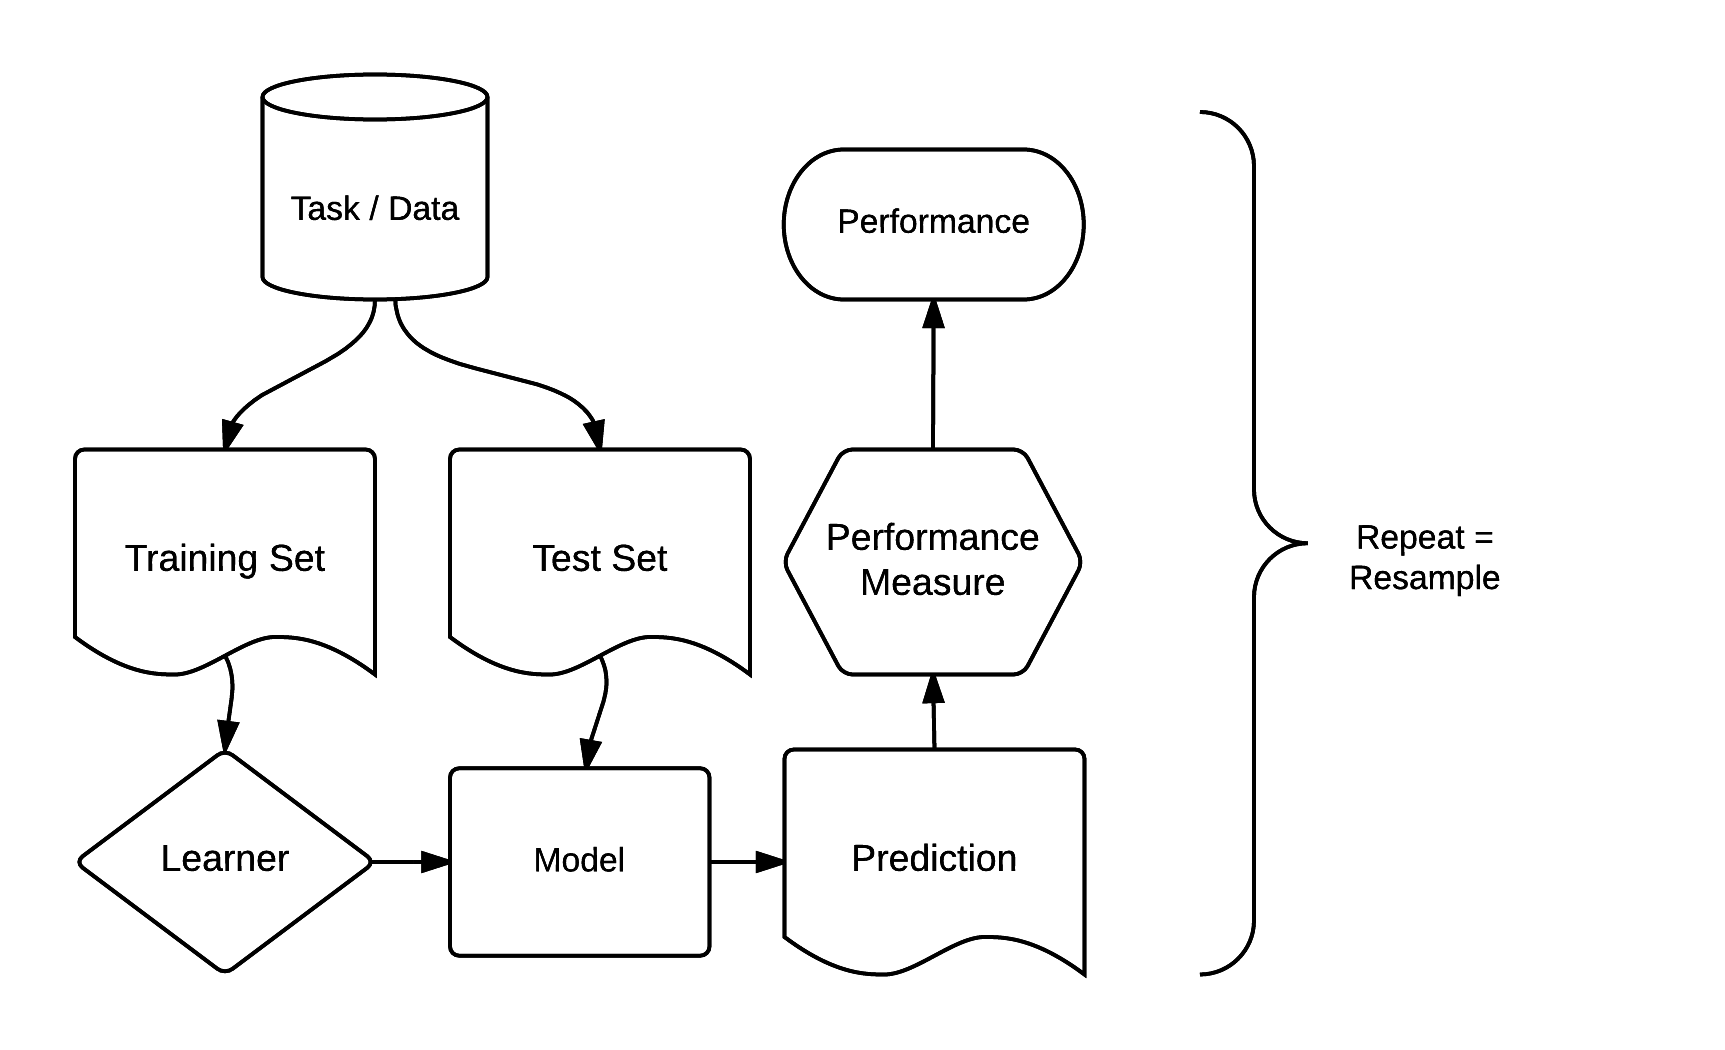
\includegraphics{images/ml_abstraction} \end{center}

The data, which \href{https://mlr3.mlr-org.com}{mlr3} encapsulates in \protect\hyperlink{tasks}{tasks}, is split into non-overlapping training and test sets.
We are interested in models that generalize to new data rather than just memorizing the training data, and separate test data allows to objectively evaluate models with respect to that.
The training data is given to a machine learning algorithm, which we call a \protect\hyperlink{learners}{learner} in \href{https://mlr3.mlr-org.com}{mlr3}.
The \protect\hyperlink{learners}{learner} uses the training data to build a model of the relationship of in the input features to the output target values.
This model is then used to produce \protect\hyperlink{predicting}{predictions} on the test data, which are compared to the ground truth values to assess the quality of the model.
\href{https://mlr3.mlr-org.com}{mlr3} offers a number of different \protect\hyperlink{measure}{measures} to quantify how well a model does based on the difference between predicted and actual values.
Usually this \protect\hyperlink{measure}{measure} is a numeric score.

The process of splitting up data into training and test sets, building a model, and evaluating it may be repeated several times, \protect\hyperlink{resampling}{resampling} different training and test sets from the original data each time.
Multiple \protect\hyperlink{resampling}{resampling iterations} iterations allow us to get a better generalization performance estimate for a particular type of model as it is tested under different conditions and less likely to get lucky or unlucky because of a particular way the data was resampled.

In many cases, this simple workflow is not sufficient to deal with real-world data, which may require normalization, imputation of missing values, or feature selection.
We will cover more complex workflows that allow to do this and even more later in the book.

This chapter covers the following subtopics:

\protect\hyperlink{tasks}{\textbf{Tasks}}

Tasks encapsulate the data with meta-information, such as what the prediction target is.
We cover how to

\begin{itemize}
\tightlist
\item
  access \protect\hyperlink{tasks-predefined}{predefined tasks},
\item
  specify a \protect\hyperlink{tasks-types}{task type},
\item
  create a \protect\hyperlink{tasks-creation}{task},
\item
  work with a task's \protect\hyperlink{tasks-api}{API},
\item
  assign roles to \protect\hyperlink{tasks-roles}{rows and collums} of a task,
\item
  implement \protect\hyperlink{tasks-mutators}{task mutators}, and
\item
  \protect\hyperlink{tasks-retrieved}{retrieve the data} that is stored in a task.
\end{itemize}

\protect\hyperlink{learners}{\textbf{Learners}}

\protect\hyperlink{learners}{Learners} encapsulate machine learning algorithms to train models and make predictions for a \texttt{mlr3::Task}.
They are provided by R and other packages.
We cover how to

\begin{itemize}
\tightlist
\item
  access the set of \protect\hyperlink{learners-predefined}{classification and regression learners} that come with mlr3 and retrieve a specific learner,
\item
  access the set of \protect\hyperlink{learners-predefined}{hyperparameter values} of a learner and modify them.
\end{itemize}

How to modify and extend learners is covered in a supplemental \protect\hyperlink{ext-learner}{advanced technical section}.

\protect\hyperlink{train-predict}{\textbf{Train and predict}}

The section on the \protect\hyperlink{train-predict}{train and predict methods} illustrates how to use \protect\hyperlink{tasks}{tasks} and \protect\hyperlink{learners}{learners} to train a model and make \protect\hyperlink{predicting}{predictions} on a new data set.
In particular, we cover how to

\begin{itemize}
\tightlist
\item
  set up \protect\hyperlink{train-predict-objects}{tasks} and \protect\hyperlink{train-predict-objects}{learners} properly,
\item
  set up \protect\hyperlink{split-data}{train and test splits} for a task,
\item
  \protect\hyperlink{training}{train} the learner on the training set to produce a model,
\item
  generate \protect\hyperlink{predicting}{predictions} on the test set, and
\item
  assess the \protect\hyperlink{measure}{performance} of the model by comparing predicted and actual values.
\end{itemize}

\protect\hyperlink{resampling}{\textbf{Resampling}}

A \protect\hyperlink{resampling}{resampling} is a method to create training and test splits.
We cover how to

\begin{itemize}
\tightlist
\item
  access and select \protect\hyperlink{resamp-settings}{resampling strategies},
\item
  instantiate the \protect\hyperlink{resamp-inst}{split into training and test sets} by applying the resampling, and
\item
  execute the resampling to obtain \protect\hyperlink{resamp-exec}{results}.
\end{itemize}

Additional information on resampling can be found in section about \protect\hyperlink{nested-resampling}{nested resampling} in the chapter on \protect\hyperlink{model-optim}{model optimization}.

\protect\hyperlink{benchmarking}{\textbf{Benchmarking}}

\protect\hyperlink{benchmarking}{Benchmarking} is used to compare the performance of different models, for example models trained with different learners, on different tasks, or with different resampling schemes.
We cover how to

\begin{itemize}
\tightlist
\item
  create a \protect\hyperlink{bm-design}{benchmarking design},
\item
  \protect\hyperlink{bm-exec}{execute a design} and aggregate results, and
\item
  convert benchmarking objects to \protect\hyperlink{bm-resamp}{resample objects}.
\end{itemize}

\protect\hyperlink{binary}{\textbf{Binary classification}}

\protect\hyperlink{binary}{Binary classification} is a special case of classification where the target variable to predict has only two possible values.
In this case, additional considerations apply; in particular

\begin{itemize}
\tightlist
\item
  \protect\hyperlink{binary-roc}{ROC curves} and the threshold where to predict one class versus the other, and
\item
  threshold tuning (WIP).
\end{itemize}

Before we get into the details of how to use \href{https://mlr3.mlr-org.com}{mlr3} for machine learning, we give a brief introduction to R6 as it is a relatively new part of R.
\href{https://mlr3.mlr-org.com}{mlr3} heavily relies on R6 and all basic building blocks it provides are R6 classes:

\begin{itemize}
\tightlist
\item
  \protect\hyperlink{tasks}{tasks},
\item
  \protect\hyperlink{learners}{learners},
\item
  \protect\hyperlink{measures}{measures}, and
\item
  \protect\hyperlink{resampling}{resamplings}.
\end{itemize}

\hypertarget{r6}{%
\section{Quick R6 Intro for Beginners}\label{r6}}

R6 is one of R's more recent dialects for object-oriented programming (OO).
It addresses shortcomings of earlier OO implementations in R, such as S3, which we used in \texttt{mlr}.
If you have done any object-oriented programming before, R6 should feel familiar.
We focus on the parts of R6 that you need to know to use \href{https://mlr3.mlr-org.com}{mlr3} here.

\begin{itemize}
\tightlist
\item
  Objects are created by calling the constructor of an \texttt{R6Class()} object, specifically the \texttt{\$new()} method.
  For example, \texttt{foo\ =\ Foo\$new(bar\ =\ 1)} creates a new object of class \texttt{Foo}, setting the \texttt{bar} argument of the constructor to \texttt{1}.
\item
  Classes have mutable state, which is encapsulated in their fields, which can be accessed through the dollar operator.
  We can access the \texttt{bar} value in the \texttt{Foo} class through \texttt{foo\$bar} and set its value by assigning the field, e.g. \texttt{foo\$bar\ =\ 2}.
\item
  In addition to fields, objects expose methods that may allow to inspect the object's state, retrieve information, or perform an action that may change the internal state of the object.
  For example, the \texttt{\$train} method of a learner changes the internal state of the learner by building and storing a trained model, which can then be used to make predictions given data.
\item
  Objects can have public and private fields and methods.
  In \href{https://mlr3.mlr-org.com}{mlr3}, you can only access the public variables and methods.
  Private fields and methods are only relevant to change or extend \href{https://mlr3.mlr-org.com}{mlr3}.
\item
  R6 variables are references to objects rather then the actual objects, which are stored in an environment.
  For example \texttt{foo2\ =\ foo} does not create a copy of \texttt{foo} in \texttt{foo2}, but another reference to the same actual object.
  Setting \texttt{foo\$bar\ =\ 3} will also change \texttt{foo2\$bar} to \texttt{3} and vice versa.
\item
  To copy an object, use the \texttt{\$clone()} method and the \texttt{deep\ =\ TRUE} argument for nested objects, for example \texttt{foo2\ =\ foo\$clone(deep\ =\ TRUE)}.
\end{itemize}

For more details on R6, have a look at the \href{https://r6.r-lib.org/}{R6 vignettes}.

\hypertarget{tasks}{%
\section{Tasks}\label{tasks}}

Tasks are objects for the data and additional meta-data for a machine learning problem.
The meta-data is for example the name of the target variable (the prediction) for supervised machine learning problems, or the type of the dataset (e.g.~a \emph{spatial} or \emph{survival}).
This information is used for specific operations that can be performed on a task.

\hypertarget{tasks-types}{%
\subsection{Task Types}\label{tasks-types}}

To create a task from a \texttt{data.frame()} or \texttt{data.table()} object, the task type needs to be specified:

\textbf{Classification Task}: The target is a label (stored as \texttt{character()}or\texttt{factor()}) with only few distinct values.
→ \texttt{mlr3::TaskClassif}

\textbf{Regression Task}: The target is a numeric quantity (stored as \texttt{integer()} or \texttt{double()}).
→ \texttt{mlr3::TaskRegr}

\textbf{Survival Task}: The target is the (right-censored) time to an event.
→ \texttt{mlr3proba::TaskSurv} in add-on package \href{https://mlr3proba.mlr-org.com}{mlr3proba}

\textbf{Ordinal Regression Task}: The target is ordinal.
→ \texttt{mlr3ordinal::TaskOrdinal} in add-on package \href{https://mlr3ordinal.mlr-org.com}{mlr3ordinal}

\textbf{Cluster Task}: An unsupervised task type; there is no target and the aim is to identify similar groups within the feature space.
→ Not yet implemented

\textbf{Spatial Task}: Observations in the task have spatio-temporal information (e.g.~coordinates).
→ Not yet implemented, but started in add-on package \href{https://mlr3spatiotempcv.mlr-org.com}{mlr3spatiotempcv}

\hypertarget{tasks-creation}{%
\subsection{Task Creation}\label{tasks-creation}}

As an example, we will create a regression task using the \texttt{mtcars} data set from the package \texttt{datasets} and predict the target \texttt{"mpg"} (miles per gallon).
We only consider the first two features in the dataset for brevity.

First, we load and prepare the data.

\begin{Shaded}
\begin{Highlighting}[]
\KeywordTok{data}\NormalTok{(}\StringTok{"mtcars"}\NormalTok{, }\DataTypeTok{package =} \StringTok{"datasets"}\NormalTok{)}
\NormalTok{data =}\StringTok{ }\NormalTok{mtcars[, }\DecValTok{1}\OperatorTok{:}\DecValTok{3}\NormalTok{]}
\KeywordTok{str}\NormalTok{(data)}
\NormalTok{## 'data.frame':    32 obs. of  3 variables:}
\NormalTok{##  $ mpg : num  21 21 22.8 21.4 18.7 18.1 14.3 24.4 22.8 19.2 ...}
\NormalTok{##  $ cyl : num  6 6 4 6 8 6 8 4 4 6 ...}
\NormalTok{##  $ disp: num  160 160 108 258 360 ...}
\end{Highlighting}
\end{Shaded}

Next, we create the task using the constructor for a regression task object (\texttt{TaskRegr\$new}) and give the following information:

\begin{enumerate}
\def\labelenumi{\arabic{enumi}.}
\tightlist
\item
  \texttt{id}: An arbitrary identifier for the task, used in plots and summaries.
\item
  \texttt{backend}: This parameter allows fine-grained control over how data is accessed.
  Here, we simply provide the dataset which is automatically converted to a \texttt{DataBackendDataTable}.
  We could also construct a \texttt{DataBackend} manually.
\item
  \texttt{target}: The name of the target column for the regression problem.
\end{enumerate}

\begin{Shaded}
\begin{Highlighting}[]
\KeywordTok{library}\NormalTok{(mlr3)}

\NormalTok{task_mtcars =}\StringTok{ }\NormalTok{TaskRegr}\OperatorTok{$}\KeywordTok{new}\NormalTok{(}\DataTypeTok{id =} \StringTok{"cars"}\NormalTok{, }\DataTypeTok{backend =}\NormalTok{ data, }\DataTypeTok{target =} \StringTok{"mpg"}\NormalTok{)}
\KeywordTok{print}\NormalTok{(task_mtcars)}
\NormalTok{## <TaskRegr:cars> (32 x 3)}
\NormalTok{## * Target: mpg}
\NormalTok{## * Properties: -}
\NormalTok{## * Features (2):}
\NormalTok{##   - dbl (2): cyl, disp}
\end{Highlighting}
\end{Shaded}

The \texttt{print()} method gives a short summary of the task:
It has 32 observations and 3 columns, of which 2 are features.

We can also plot the task using the \href{https://mlr3viz.mlr-org.com}{mlr3viz} package, which gives a graphical summary of its properties:

\begin{Shaded}
\begin{Highlighting}[]
\KeywordTok{library}\NormalTok{(mlr3viz)}
\KeywordTok{autoplot}\NormalTok{(task_mtcars, }\DataTypeTok{type =} \StringTok{"pairs"}\NormalTok{)}
\end{Highlighting}
\end{Shaded}

\begin{center}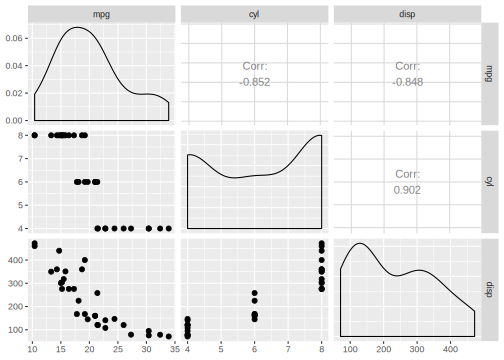
\includegraphics{mlr3book_files/figure-latex/02-basics-005-1} \end{center}

\hypertarget{tasks-predefined}{%
\subsection{Predefined tasks}\label{tasks-predefined}}

\href{https://mlr3.mlr-org.com}{mlr3} ships with a few predefined machine learning tasks.
All tasks are stored in an R6 \texttt{Dictionary} (a key-value store) named \texttt{mlr\_tasks}.
Printing it gives the keys (the names of the datasets):

\begin{Shaded}
\begin{Highlighting}[]
\NormalTok{mlr_tasks}
\NormalTok{## <DictionaryTask> with 12 stored values}
\NormalTok{## Keys: boston_housing, german_credit, iris, lung,}
\NormalTok{##   mtcars, pima, rats, sonar, spam, unemployment,}
\NormalTok{##   wine, zoo}
\end{Highlighting}
\end{Shaded}

We can get a more informative summary of the example tasks by converting the dictionary to a \texttt{data.table()} object:

\begin{Shaded}
\begin{Highlighting}[]
\KeywordTok{library}\NormalTok{(data.table)}
\KeywordTok{as.data.table}\NormalTok{(mlr_tasks)}
\NormalTok{##                key task_type nrow ncol lgl int dbl chr}
\NormalTok{##  1: boston_housing      regr  506   19   0   3  13   0}
\NormalTok{##  2:  german_credit   classif 1000   21   0   0   7   0}
\NormalTok{##  3:           iris   classif  150    5   0   0   4   0}
\NormalTok{##  4:           lung      surv  228   10   0   7   0   0}
\NormalTok{##  5:         mtcars      regr   32   11   0   0  10   0}
\NormalTok{##  6:           pima   classif  768    9   0   0   8   0}
\NormalTok{##  7:           rats      surv  300    5   0   2   0   0}
\NormalTok{##  8:          sonar   classif  208   61   0   0  60   0}
\NormalTok{##  9:           spam   classif 4601   58   0   0  57   0}
\NormalTok{## 10:   unemployment      surv 3343    6   0   1   2   0}
\NormalTok{## 11:           wine   classif  178   14   0   2  11   0}
\NormalTok{## 12:            zoo   classif  101   17  15   1   0   0}
\NormalTok{##     fct ord pxc}
\NormalTok{##  1:   2   0   0}
\NormalTok{##  2:  12   1   0}
\NormalTok{##  3:   0   0   0}
\NormalTok{##  4:   1   0   0}
\NormalTok{##  5:   0   0   0}
\NormalTok{##  6:   0   0   0}
\NormalTok{##  7:   1   0   0}
\NormalTok{##  8:   0   0   0}
\NormalTok{##  9:   0   0   0}
\NormalTok{## 10:   1   0   0}
\NormalTok{## 11:   0   0   0}
\NormalTok{## 12:   0   0   0}
\end{Highlighting}
\end{Shaded}

To get a task from the dictionary, one can use the \texttt{\$get()} method from the \texttt{mlr\_tasks} class and assign the return value to a new object.
For example, to use the \href{https://en.wikipedia.org/wiki/Iris_flower_data_set}{iris data set} for classification:

\begin{Shaded}
\begin{Highlighting}[]
\NormalTok{task_iris =}\StringTok{ }\NormalTok{mlr_tasks}\OperatorTok{$}\KeywordTok{get}\NormalTok{(}\StringTok{"iris"}\NormalTok{)}
\KeywordTok{print}\NormalTok{(task_iris)}
\NormalTok{## <TaskClassif:iris> (150 x 5)}
\NormalTok{## * Target: Species}
\NormalTok{## * Properties: multiclass}
\NormalTok{## * Features (4):}
\NormalTok{##   - dbl (4): Petal.Length, Petal.Width,}
\NormalTok{##     Sepal.Length, Sepal.Width}
\end{Highlighting}
\end{Shaded}

Alternatively, you can also use the convenience function \texttt{tsk()}, which also constructs a task from the dictionary.

\begin{Shaded}
\begin{Highlighting}[]
\KeywordTok{tsk}\NormalTok{(}\StringTok{"iris"}\NormalTok{)}
\NormalTok{## <TaskClassif:iris> (150 x 5)}
\NormalTok{## * Target: Species}
\NormalTok{## * Properties: multiclass}
\NormalTok{## * Features (4):}
\NormalTok{##   - dbl (4): Petal.Length, Petal.Width,}
\NormalTok{##     Sepal.Length, Sepal.Width}
\end{Highlighting}
\end{Shaded}

\hypertarget{tasks-api}{%
\subsection{Task API}\label{tasks-api}}

All task properties and characteristics can be queried using the task's public fields and methods (see \texttt{Task}).
Methods are also used to change the behavior of the task.

\hypertarget{tasks-retrieving}{%
\subsubsection{Retrieving Data}\label{tasks-retrieving}}

The data stored in a task can be retrieved directly from fields, for example:

\begin{Shaded}
\begin{Highlighting}[]
\NormalTok{task_iris}\OperatorTok{$}\NormalTok{nrow}
\NormalTok{## [1] 150}
\NormalTok{task_iris}\OperatorTok{$}\NormalTok{ncol}
\NormalTok{## [1] 5}
\end{Highlighting}
\end{Shaded}

More information can be obtained through methods of the object, for example:

\begin{Shaded}
\begin{Highlighting}[]
\NormalTok{task_iris}\OperatorTok{$}\KeywordTok{data}\NormalTok{()}
\NormalTok{##        Species Petal.Length Petal.Width Sepal.Length}
\NormalTok{##   1:    setosa          1.4         0.2          5.1}
\NormalTok{##   2:    setosa          1.4         0.2          4.9}
\NormalTok{##   3:    setosa          1.3         0.2          4.7}
\NormalTok{##   4:    setosa          1.5         0.2          4.6}
\NormalTok{##   5:    setosa          1.4         0.2          5.0}
\NormalTok{##  ---                                                }
\NormalTok{## 146: virginica          5.2         2.3          6.7}
\NormalTok{## 147: virginica          5.0         1.9          6.3}
\NormalTok{## 148: virginica          5.2         2.0          6.5}
\NormalTok{## 149: virginica          5.4         2.3          6.2}
\NormalTok{## 150: virginica          5.1         1.8          5.9}
\NormalTok{##      Sepal.Width}
\NormalTok{##   1:         3.5}
\NormalTok{##   2:         3.0}
\NormalTok{##   3:         3.2}
\NormalTok{##   4:         3.1}
\NormalTok{##   5:         3.6}
\NormalTok{##  ---            }
\NormalTok{## 146:         3.0}
\NormalTok{## 147:         2.5}
\NormalTok{## 148:         3.0}
\NormalTok{## 149:         3.4}
\NormalTok{## 150:         3.0}
\end{Highlighting}
\end{Shaded}

In \href{https://mlr3.mlr-org.com}{mlr3}, each row (observation) has a unique identifier.
The identifier is either an \texttt{integer} or \texttt{character}.
These can be passed as arguments to the \texttt{\$data()} method to select specific rows.

The \emph{iris} task uses integer \texttt{row\_ids}:

\begin{Shaded}
\begin{Highlighting}[]
\CommentTok{# iris uses integer row_ids}
\KeywordTok{head}\NormalTok{(task_iris}\OperatorTok{$}\NormalTok{row_ids)}
\NormalTok{## [1] 1 2 3 4 5 6}

\CommentTok{# retrieve data for rows with ids 1, 51, and 101}
\NormalTok{task_iris}\OperatorTok{$}\KeywordTok{data}\NormalTok{(}\DataTypeTok{rows =} \KeywordTok{c}\NormalTok{(}\DecValTok{1}\NormalTok{, }\DecValTok{51}\NormalTok{, }\DecValTok{101}\NormalTok{))}
\NormalTok{##       Species Petal.Length Petal.Width Sepal.Length}
\NormalTok{## 1:     setosa          1.4         0.2          5.1}
\NormalTok{## 2: versicolor          4.7         1.4          7.0}
\NormalTok{## 3:  virginica          6.0         2.5          6.3}
\NormalTok{##    Sepal.Width}
\NormalTok{## 1:         3.5}
\NormalTok{## 2:         3.2}
\NormalTok{## 3:         3.3}
\end{Highlighting}
\end{Shaded}

The \emph{mtcars} task on the other hand uses names for its \texttt{row\_ids}, encoded as \texttt{character}:

\begin{Shaded}
\begin{Highlighting}[]
\NormalTok{task_mtcars =}\StringTok{ }\KeywordTok{tsk}\NormalTok{(}\StringTok{"mtcars"}\NormalTok{)}
\KeywordTok{head}\NormalTok{(task_mtcars}\OperatorTok{$}\NormalTok{row_ids)}
\NormalTok{## [1] "AMC Javelin"        "Cadillac Fleetwood"}
\NormalTok{## [3] "Camaro Z28"         "Chrysler Imperial" }
\NormalTok{## [5] "Datsun 710"         "Dodge Challenger"}

\CommentTok{# retrieve data for rows with id 'Datsun 710'}
\NormalTok{task_mtcars}\OperatorTok{$}\KeywordTok{data}\NormalTok{(}\DataTypeTok{rows =} \StringTok{"Datsun 710"}\NormalTok{)}
\NormalTok{##     mpg am carb cyl disp drat gear hp  qsec vs   wt}
\NormalTok{## 1: 22.8  1    1   4  108 3.85    4 93 18.61  1 2.32}
\end{Highlighting}
\end{Shaded}

Note that the method \texttt{\$data()} only allows to read the data and does not modify it.

Similarly, each column has an identifier or name.
These names are stored in the public slots \texttt{feature\_names} and \texttt{target\_names}.
Here ``target'' refers to the variable we want to predict and ``feature'' to the predictors for the task.

\begin{Shaded}
\begin{Highlighting}[]
\NormalTok{task_iris}\OperatorTok{$}\NormalTok{feature_names}
\NormalTok{## [1] "Petal.Length" "Petal.Width"  "Sepal.Length"}
\NormalTok{## [4] "Sepal.Width"}
\NormalTok{task_iris}\OperatorTok{$}\NormalTok{target_names}
\NormalTok{## [1] "Species"}
\end{Highlighting}
\end{Shaded}

The \texttt{row\_id}s and column names can be combined when selecting a subset of the data:

\begin{Shaded}
\begin{Highlighting}[]
\CommentTok{# retrieve data for rows 1, 51, and 101 and only select}
\CommentTok{# column 'Species'}
\NormalTok{task_iris}\OperatorTok{$}\KeywordTok{data}\NormalTok{(}\DataTypeTok{rows =} \KeywordTok{c}\NormalTok{(}\DecValTok{1}\NormalTok{, }\DecValTok{51}\NormalTok{, }\DecValTok{101}\NormalTok{), }\DataTypeTok{cols =} \StringTok{"Species"}\NormalTok{)}
\NormalTok{##       Species}
\NormalTok{## 1:     setosa}
\NormalTok{## 2: versicolor}
\NormalTok{## 3:  virginica}
\end{Highlighting}
\end{Shaded}

To extract the complete data from the task, one can simply convert it to a \texttt{data.table}:

\begin{Shaded}
\begin{Highlighting}[]
\KeywordTok{summary}\NormalTok{(}\KeywordTok{as.data.table}\NormalTok{(task_iris))}
\NormalTok{##        Species    Petal.Length   Petal.Width }
\NormalTok{##  setosa    :50   Min.   :1.00   Min.   :0.1  }
\NormalTok{##  versicolor:50   1st Qu.:1.60   1st Qu.:0.3  }
\NormalTok{##  virginica :50   Median :4.35   Median :1.3  }
\NormalTok{##                  Mean   :3.76   Mean   :1.2  }
\NormalTok{##                  3rd Qu.:5.10   3rd Qu.:1.8  }
\NormalTok{##                  Max.   :6.90   Max.   :2.5  }
\NormalTok{##   Sepal.Length   Sepal.Width  }
\NormalTok{##  Min.   :4.30   Min.   :2.00  }
\NormalTok{##  1st Qu.:5.10   1st Qu.:2.80  }
\NormalTok{##  Median :5.80   Median :3.00  }
\NormalTok{##  Mean   :5.84   Mean   :3.06  }
\NormalTok{##  3rd Qu.:6.40   3rd Qu.:3.30  }
\NormalTok{##  Max.   :7.90   Max.   :4.40}
\end{Highlighting}
\end{Shaded}

\hypertarget{tasks-roles}{%
\subsubsection{Roles (Rows and Columns)}\label{tasks-roles}}

It is possible to assign roles to rows and columns.
These roles affect the behavior of the task for different operations.
Furthermore, these roles provide additional meta-data for it.

For example, the previously-constructed \emph{mtcars} task has the following column roles:

\begin{Shaded}
\begin{Highlighting}[]
\KeywordTok{print}\NormalTok{(task_mtcars}\OperatorTok{$}\NormalTok{col_roles)}
\NormalTok{## $feature}
\NormalTok{##  [1] "am"   "carb" "cyl"  "disp" "drat" "gear" "hp"  }
\NormalTok{##  [8] "qsec" "vs"   "wt"  }
\NormalTok{## }
\NormalTok{## $target}
\NormalTok{## [1] "mpg"}
\NormalTok{## }
\NormalTok{## $name}
\NormalTok{## character(0)}
\NormalTok{## }
\NormalTok{## $order}
\NormalTok{## character(0)}
\NormalTok{## }
\NormalTok{## $stratum}
\NormalTok{## character(0)}
\NormalTok{## }
\NormalTok{## $group}
\NormalTok{## character(0)}
\NormalTok{## }
\NormalTok{## $weight}
\NormalTok{## character(0)}
\end{Highlighting}
\end{Shaded}

To add the row names of \texttt{mtcars} as an additional feature, we first add them to the data table and then recreate the task.

\begin{Shaded}
\begin{Highlighting}[]
\CommentTok{# with `keep.rownames`, data.table stores the row names}
\CommentTok{# in an extra column 'rn'}
\NormalTok{data =}\StringTok{ }\KeywordTok{as.data.table}\NormalTok{(mtcars[, }\DecValTok{1}\OperatorTok{:}\DecValTok{3}\NormalTok{], }\DataTypeTok{keep.rownames =} \OtherTok{TRUE}\NormalTok{)}
\NormalTok{task =}\StringTok{ }\NormalTok{TaskRegr}\OperatorTok{$}\KeywordTok{new}\NormalTok{(}\DataTypeTok{id =} \StringTok{"cars"}\NormalTok{, }\DataTypeTok{backend =}\NormalTok{ data, }\DataTypeTok{target =} \StringTok{"mpg"}\NormalTok{)}

\CommentTok{# we now have integer row_ids}
\NormalTok{task}\OperatorTok{$}\NormalTok{row_ids}
\NormalTok{##  [1]  1  2  3  4  5  6  7  8  9 10 11 12 13 14 15 16 17}
\NormalTok{## [18] 18 19 20 21 22 23 24 25 26 27 28 29 30 31 32}

\CommentTok{# there is a new feature called 'rn'}
\NormalTok{task}\OperatorTok{$}\NormalTok{feature_names}
\NormalTok{## [1] "cyl"  "disp" "rn"}
\end{Highlighting}
\end{Shaded}

The row names are now a feature whose values are stored in the column ``rn''.
We include this column here for educational purposes only.
Generally speaking, there is no point in having a feature that uniquely identifies each row.
Furthermore, the character data type will cause problems with many types of machine learning algorithms.
The identifier may be useful to label points in plots and identify outliers however.
To use the new column for only this purpose, we will change the role of the ``rn'' column and remove it from the set of active features.

\begin{Shaded}
\begin{Highlighting}[]
\NormalTok{task}\OperatorTok{$}\NormalTok{feature_names}
\NormalTok{## [1] "cyl"  "disp" "rn"}

\CommentTok{# working with a list of column vectors}
\NormalTok{task}\OperatorTok{$}\NormalTok{col_roles}\OperatorTok{$}\NormalTok{name =}\StringTok{ "rn"}
\NormalTok{task}\OperatorTok{$}\NormalTok{col_roles}\OperatorTok{$}\NormalTok{feature =}\StringTok{ }\KeywordTok{setdiff}\NormalTok{(task}\OperatorTok{$}\NormalTok{col_roles}\OperatorTok{$}\NormalTok{feature, }
  \StringTok{"rn"}\NormalTok{)}

\CommentTok{# 'rn' not listed as feature anymore}
\NormalTok{task}\OperatorTok{$}\NormalTok{feature_names}
\NormalTok{## [1] "cyl"  "disp"}

\CommentTok{# does also not appear when we access the data anymore}
\NormalTok{task}\OperatorTok{$}\KeywordTok{data}\NormalTok{(}\DataTypeTok{rows =} \DecValTok{1}\OperatorTok{:}\DecValTok{2}\NormalTok{)}
\NormalTok{##    mpg cyl disp}
\NormalTok{## 1:  21   6  160}
\NormalTok{## 2:  21   6  160}
\NormalTok{task}\OperatorTok{$}\KeywordTok{head}\NormalTok{(}\DecValTok{2}\NormalTok{)}
\NormalTok{##    mpg cyl disp}
\NormalTok{## 1:  21   6  160}
\NormalTok{## 2:  21   6  160}
\end{Highlighting}
\end{Shaded}

Changing the role does not change the underlying data.
Changing the role only changes the view on it.
The data is not copied in the code above.
The view is changed in-place though, i.e.~the task object itself is modified.

Just like columns, it is also possible to assign different roles to rows.
Rows can have two different roles:

\begin{enumerate}
\def\labelenumi{\arabic{enumi}.}
\item
  Role \texttt{use}
  Rows that are generally available for model fitting (although they may also be used as test set in resampling).
  This role is the default role.
\item
  Role \texttt{validation}
  Rows that are not used for training.
  Rows that have missing values in the target column during task creation are automatically set to the validation role.
\end{enumerate}

There are several reasons to hold some observations back or treat them differently:

\begin{enumerate}
\def\labelenumi{\arabic{enumi}.}
\tightlist
\item
  It is often good practice to validate the final model on an external validation set to identify possible overfitting.
\item
  Some observations may be unlabeled, e.g.~in competitions like \href{https://www.kaggle.com/}{Kaggle}.
\end{enumerate}

These observations cannot be used for training a model, but can be used to get predictions.

\hypertarget{tasks-mutators}{%
\subsubsection{Task Mutators}\label{tasks-mutators}}

As shown above, modifying \texttt{\$col\_roles} or \texttt{\$row\_roles} changes the view on the data.
The additional convenience method \texttt{\$filter()} subsets the current view based on row ids and \texttt{\$select()} subsets the view based on feature names.

\begin{Shaded}
\begin{Highlighting}[]
\NormalTok{task =}\StringTok{ }\KeywordTok{tsk}\NormalTok{(}\StringTok{"iris"}\NormalTok{)}
\NormalTok{task}\OperatorTok{$}\KeywordTok{select}\NormalTok{(}\KeywordTok{c}\NormalTok{(}\StringTok{"Sepal.Width"}\NormalTok{, }\StringTok{"Sepal.Length"}\NormalTok{))  }\CommentTok{# keep only these features}
\NormalTok{task}\OperatorTok{$}\KeywordTok{filter}\NormalTok{(}\DecValTok{1}\OperatorTok{:}\DecValTok{3}\NormalTok{)  }\CommentTok{# keep only these rows}
\NormalTok{task}\OperatorTok{$}\KeywordTok{head}\NormalTok{()}
\NormalTok{##    Species Sepal.Length Sepal.Width}
\NormalTok{## 1:  setosa          5.1         3.5}
\NormalTok{## 2:  setosa          4.9         3.0}
\NormalTok{## 3:  setosa          4.7         3.2}
\end{Highlighting}
\end{Shaded}

While the methods discussed above allow to subset the data, the methods \texttt{\$rbind()} and \texttt{\$cbind()} allow to add extra rows and columns to a task.
Again, the original data is not changed.
The additional rows or columns are only added to the view of the data.

\begin{Shaded}
\begin{Highlighting}[]
\NormalTok{task}\OperatorTok{$}\KeywordTok{cbind}\NormalTok{(}\KeywordTok{data.table}\NormalTok{(}\DataTypeTok{foo =}\NormalTok{ letters[}\DecValTok{1}\OperatorTok{:}\DecValTok{3}\NormalTok{]))  }\CommentTok{# add column foo}
\NormalTok{task}\OperatorTok{$}\KeywordTok{head}\NormalTok{()}
\NormalTok{##    Species Sepal.Length Sepal.Width foo}
\NormalTok{## 1:  setosa          5.1         3.5   a}
\NormalTok{## 2:  setosa          4.9         3.0   b}
\NormalTok{## 3:  setosa          4.7         3.2   c}
\end{Highlighting}
\end{Shaded}

\hypertarget{autoplot-task}{%
\subsection{Plotting Tasks}\label{autoplot-task}}

The \href{https://mlr3viz.mlr-org.com}{mlr3viz} provides plotting facilities for many classes implemented in \href{https://mlr3.mlr-org.com}{mlr3}.
The types of plot depend on the inherited class, but all plots are returned as \texttt{ggplot2} objects which can be easily customized.

For for classification tasks (inheriting from \texttt{TaskClassif}), see the documentation of \texttt{mlr3viz::autoplot.TaskClassif} for the implemented plot types.
Here are some examples to get an impression:

\begin{Shaded}
\begin{Highlighting}[]
\KeywordTok{library}\NormalTok{(mlr3viz)}

\CommentTok{# get the pima indians task}
\NormalTok{task =}\StringTok{ }\KeywordTok{tsk}\NormalTok{(}\StringTok{"pima"}\NormalTok{)}

\CommentTok{# subset task to only use the 3 first features}
\NormalTok{task}\OperatorTok{$}\KeywordTok{select}\NormalTok{(}\KeywordTok{head}\NormalTok{(task}\OperatorTok{$}\NormalTok{feature_names, }\DecValTok{3}\NormalTok{))}

\CommentTok{# default plot: class frequencies}
\KeywordTok{autoplot}\NormalTok{(task)}
\end{Highlighting}
\end{Shaded}

\begin{center}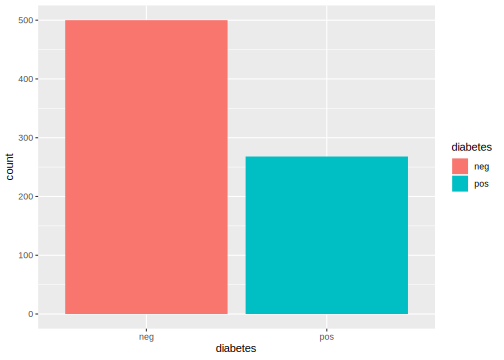
\includegraphics{mlr3book_files/figure-latex/02-basics-022-1} \end{center}

\begin{Shaded}
\begin{Highlighting}[]

\CommentTok{# pairs plot (requires package GGally)}
\KeywordTok{autoplot}\NormalTok{(task, }\DataTypeTok{type =} \StringTok{"pairs"}\NormalTok{)}
\end{Highlighting}
\end{Shaded}

\begin{center}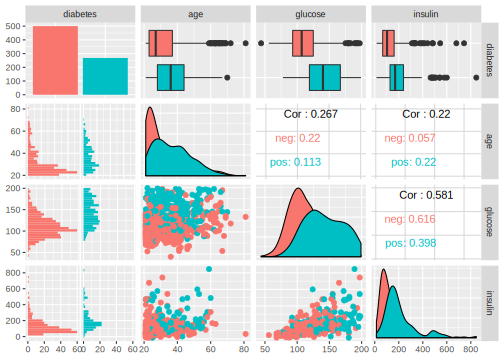
\includegraphics{mlr3book_files/figure-latex/02-basics-022-2} \end{center}

\begin{Shaded}
\begin{Highlighting}[]

\CommentTok{# duo plot (requires package GGally)}
\KeywordTok{autoplot}\NormalTok{(task, }\DataTypeTok{type =} \StringTok{"duo"}\NormalTok{)}
\end{Highlighting}
\end{Shaded}

\begin{center}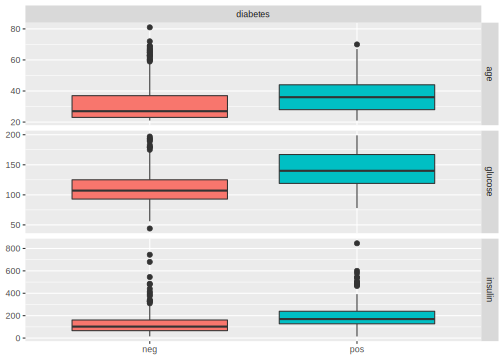
\includegraphics{mlr3book_files/figure-latex/02-basics-022-3} \end{center}

Of course, you can do the same for regression tasks (inheriting from \texttt{TaskRegr}) as documented in \texttt{mlr3viz::autoplot.TaskRegr}:

\begin{Shaded}
\begin{Highlighting}[]
\KeywordTok{library}\NormalTok{(mlr3viz)}

\CommentTok{# get the boston housing task}
\NormalTok{task =}\StringTok{ }\KeywordTok{tsk}\NormalTok{(}\StringTok{"mtcars"}\NormalTok{)}

\CommentTok{# subset task to only use the 3 first features}
\NormalTok{task}\OperatorTok{$}\KeywordTok{select}\NormalTok{(}\KeywordTok{head}\NormalTok{(task}\OperatorTok{$}\NormalTok{feature_names, }\DecValTok{3}\NormalTok{))}

\CommentTok{# default plot: boxplot of target variable}
\KeywordTok{autoplot}\NormalTok{(task)}
\end{Highlighting}
\end{Shaded}

\begin{center}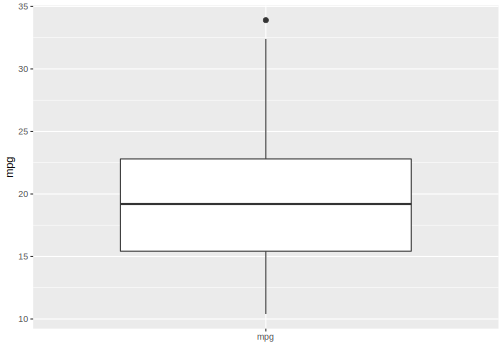
\includegraphics{mlr3book_files/figure-latex/02-basics-023-1} \end{center}

\begin{Shaded}
\begin{Highlighting}[]

\CommentTok{# pairs plot (requires package GGally)}
\KeywordTok{autoplot}\NormalTok{(task, }\DataTypeTok{type =} \StringTok{"pairs"}\NormalTok{)}
\end{Highlighting}
\end{Shaded}

\begin{center}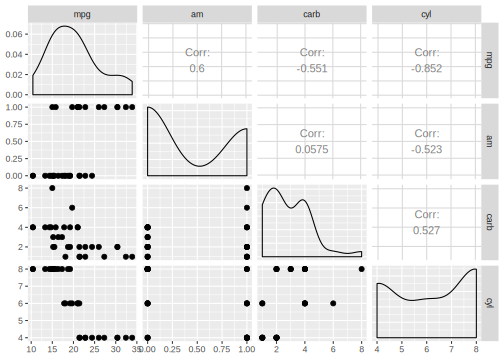
\includegraphics{mlr3book_files/figure-latex/02-basics-023-2} \end{center}

\hypertarget{learners}{%
\section{Learners}\label{learners}}

Objects of class \texttt{mlr3::Learner} provide a unified interface to many popular machine learning algorithms in R.
They consist of methods to train and predict a model for a \texttt{mlr3::Task} and provide meta-information about the learners, such as the hyperparameters you can set.

The package ships with a minimal set of classification and regression learners to avoid lots of dependencies:

\begin{itemize}
\tightlist
\item
  \texttt{mlr\_learners\_classif.featureless}: Simple baseline classification learner, constantly predicts the label most most frequent label.
\item
  \texttt{mlr\_learners\_classif.rpart}: Single classification tree from \texttt{rpart}.
\item
  \texttt{mlr\_learners\_regr.featureless}: Simple baseline regression learner, constantly predicts with the mean.
\item
  \texttt{mlr\_learners\_regr.rpart}: Single regression tree from \texttt{rpart}.
\end{itemize}

Some of the most popular learners are connected via the \href{https://mlr3learners.mlr-org.com}{mlr3learners} package:

\begin{itemize}
\tightlist
\item
  (penalized) linear and logistic regression
\item
  \(k\)-Nearest Neighbors regression and classification
\item
  Linear and Quadratic Discriminant Analysis
\item
  Naive Bayes
\item
  Support-Vector machines
\item
  Gradient Boosting
\item
  Random Regression Forests and Random Classification Forests
\item
  Kriging
\end{itemize}

More learners are collected on GitHub in the \href{https://github.com/mlr3learners/}{mlr3learners organization}.
Their state is also listed on the \href{https://github.com/mlr-org/mlr3learners/wiki}{wiki} of the \href{https://github.com/mlr-org/mlr3learners/}{mlr3learners repository}.

The base class of each learner is \texttt{Learner}, specialized for regression as \texttt{LearnerRegr} and for classification as \texttt{LearnerClassif}.
In contrast to the \texttt{Task}, the creation of a custom Learner is usually not required and a more advanced topic.
Hence, we refer the reader to Section \ref{ext-learner} and proceed with an overview of the interface of already implemented learners.

\hypertarget{learners-predefined}{%
\subsection{Predefined Learners}\label{learners-predefined}}

Similar to \texttt{mlr\_tasks}, the \texttt{Dictionary} \texttt{mlr\_learners} can be queried for available learners:

\begin{Shaded}
\begin{Highlighting}[]
\KeywordTok{library}\NormalTok{(mlr3learners)}
\NormalTok{mlr_learners}
\NormalTok{## <DictionaryLearner> with 38 stored values}
\NormalTok{## Keys: classif.debug, classif.featureless,}
\NormalTok{##   classif.glmnet, classif.kknn, classif.lda,}
\NormalTok{##   classif.log_reg, classif.naive_bayes,}
\NormalTok{##   classif.qda, classif.ranger, classif.rpart,}
\NormalTok{##   classif.svm, classif.xgboost, regr.featureless,}
\NormalTok{##   regr.glmnet, regr.kknn, regr.km, regr.lm,}
\NormalTok{##   regr.ranger, regr.rpart, regr.svm,}
\NormalTok{##   regr.xgboost, surv.blackboost, surv.coxph,}
\NormalTok{##   surv.cvglmnet, surv.flexible, surv.gamboost,}
\NormalTok{##   surv.gbm, surv.glmboost, surv.glmnet,}
\NormalTok{##   surv.kaplan, surv.mboost, surv.nelson,}
\NormalTok{##   surv.parametric, surv.penalized,}
\NormalTok{##   surv.randomForestSRC, surv.ranger, surv.rpart,}
\NormalTok{##   surv.svm}
\end{Highlighting}
\end{Shaded}

Each learner has the following information:

\begin{itemize}
\tightlist
\item
  \texttt{feature\_types}: the type of features the learner can deal with.
\item
  \texttt{packages}: the packages required to train a model with this learner and make predictions.
\item
  \texttt{properties}: additional properties and capabilities.
  For example, a learner has the property ``missings'' if it is able to handle missing feature values, and ``importance'' if it computes and allows to extract data on the relative importance of the features.
  A complete list of these is available in the mlr3 reference on \href{https://mlr3.mlr-org.com/reference/LearnerRegr.html\#construction}{regression learners} and \href{https://mlr3.mlr-org.com/reference/LearnerClassif.html\#construction}{classification learners}.
\item
  \texttt{predict\_types}: possible prediction types. For example, a classification learner can predict labels (``response'') or probabilities (``prob''). For a complete list of possible predict types see the \href{https://mlr3.mlr-org.com/reference/Learner.html\#construction}{mlr3 reference}.
\end{itemize}

For a tabular overview of integrated learners, see Section \ref{list-learners}.

You can get a specific learner using its \texttt{id}, listed under \texttt{key} in the dictionary:

\begin{Shaded}
\begin{Highlighting}[]
\NormalTok{learner =}\StringTok{ }\NormalTok{mlr_learners}\OperatorTok{$}\KeywordTok{get}\NormalTok{(}\StringTok{"classif.rpart"}\NormalTok{)}
\KeywordTok{print}\NormalTok{(learner)}
\NormalTok{## <LearnerClassifRpart:classif.rpart>}
\NormalTok{## * Model: -}
\NormalTok{## * Parameters: xval=0}
\NormalTok{## * Packages: rpart}
\NormalTok{## * Predict Type: response}
\NormalTok{## * Feature types: logical, integer, numeric,}
\NormalTok{##   factor, ordered}
\NormalTok{## * Properties: importance, missings, multiclass,}
\NormalTok{##   selected_features, twoclass, weights}
\end{Highlighting}
\end{Shaded}

The field \texttt{param\_set} stores a description of the hyperparameters the learner has, their ranges, defaults, and current values:

\begin{Shaded}
\begin{Highlighting}[]
\NormalTok{learner}\OperatorTok{$}\NormalTok{param_set}
\NormalTok{## ParamSet: }
\NormalTok{##              id    class lower upper levels default}
\NormalTok{## 1:     minsplit ParamInt     1   Inf             20}
\NormalTok{## 2:           cp ParamDbl     0     1           0.01}
\NormalTok{## 3:   maxcompete ParamInt     0   Inf              4}
\NormalTok{## 4: maxsurrogate ParamInt     0   Inf              5}
\NormalTok{## 5:     maxdepth ParamInt     1    30             30}
\NormalTok{## 6:         xval ParamInt     0   Inf             10}
\NormalTok{##    value}
\NormalTok{## 1:      }
\NormalTok{## 2:      }
\NormalTok{## 3:      }
\NormalTok{## 4:      }
\NormalTok{## 5:      }
\NormalTok{## 6:     0}
\end{Highlighting}
\end{Shaded}

The set of current hyperparameter values is stored in the \texttt{values} field of the \texttt{param\_set} field.
You can change the current hyperparameter values by assigning a named list to this field:

\begin{Shaded}
\begin{Highlighting}[]
\NormalTok{learner}\OperatorTok{$}\NormalTok{param_set}\OperatorTok{$}\NormalTok{values =}\StringTok{ }\KeywordTok{list}\NormalTok{(}\DataTypeTok{cp =} \FloatTok{0.01}\NormalTok{, }\DataTypeTok{xval =} \DecValTok{0}\NormalTok{)}
\NormalTok{learner}
\NormalTok{## <LearnerClassifRpart:classif.rpart>}
\NormalTok{## * Model: -}
\NormalTok{## * Parameters: cp=0.01, xval=0}
\NormalTok{## * Packages: rpart}
\NormalTok{## * Predict Type: response}
\NormalTok{## * Feature types: logical, integer, numeric,}
\NormalTok{##   factor, ordered}
\NormalTok{## * Properties: importance, missings, multiclass,}
\NormalTok{##   selected_features, twoclass, weights}
\end{Highlighting}
\end{Shaded}

Note that this operation just overwrites all previously set parameters.
If you just want to add or update hyperparameters, you can use \texttt{mlr3misc::insert\_named()}:

\begin{Shaded}
\begin{Highlighting}[]
\NormalTok{learner}\OperatorTok{$}\NormalTok{param_set}\OperatorTok{$}\NormalTok{values =}\StringTok{ }\NormalTok{mlr3misc}\OperatorTok{::}\KeywordTok{insert_named}\NormalTok{(learner}\OperatorTok{$}\NormalTok{param_set}\OperatorTok{$}\NormalTok{values, }
  \KeywordTok{list}\NormalTok{(}\DataTypeTok{cp =} \FloatTok{0.02}\NormalTok{, }\DataTypeTok{minsplit =} \DecValTok{2}\NormalTok{))}
\NormalTok{learner}
\NormalTok{## <LearnerClassifRpart:classif.rpart>}
\NormalTok{## * Model: -}
\NormalTok{## * Parameters: cp=0.02, xval=0, minsplit=2}
\NormalTok{## * Packages: rpart}
\NormalTok{## * Predict Type: response}
\NormalTok{## * Feature types: logical, integer, numeric,}
\NormalTok{##   factor, ordered}
\NormalTok{## * Properties: importance, missings, multiclass,}
\NormalTok{##   selected_features, twoclass, weights}
\end{Highlighting}
\end{Shaded}

This updates \texttt{cp} to \texttt{0.02}, sets \texttt{minsplit} to \texttt{2} and keeps the previously set parameter \texttt{xval}.

Again, there is an alternative to writing down the lengthy \texttt{mlr\_learners\$get()} part: \texttt{lrn()}.
This function additionally allows to construct learners with specific hyperparameters or settings of a different identifier in one go:

\begin{Shaded}
\begin{Highlighting}[]
\KeywordTok{lrn}\NormalTok{(}\StringTok{"classif.rpart"}\NormalTok{, }\DataTypeTok{id =} \StringTok{"rp"}\NormalTok{, }\DataTypeTok{cp =} \FloatTok{0.001}\NormalTok{)}
\NormalTok{## <LearnerClassifRpart:rp>}
\NormalTok{## * Model: -}
\NormalTok{## * Parameters: xval=0, cp=0.001}
\NormalTok{## * Packages: rpart}
\NormalTok{## * Predict Type: response}
\NormalTok{## * Feature types: logical, integer, numeric,}
\NormalTok{##   factor, ordered}
\NormalTok{## * Properties: importance, missings, multiclass,}
\NormalTok{##   selected_features, twoclass, weights}
\end{Highlighting}
\end{Shaded}

If you pass hyperparameters here, it is added to the default parameters in a \texttt{mlr3misc::insert\_named()",\ text\ =\ "insert\_named()}-fashion.

For further information on how to customize learners using mlr3, see the section on \protect\hyperlink{ext-learner}{extending learners}.

\hypertarget{train-predict}{%
\section{Train and Predict}\label{train-predict}}

In this section, we explain how \protect\hyperlink{tasks}{tasks} and \protect\hyperlink{learners}{learners} can be used to train a model and predict to a new dataset.
The concept is demonstrated on a supervised classification using the iris dataset and the \textbf{rpart} learner (classification tree).

Training a \protect\hyperlink{learners}{learner} means fitting a model to a given data set.
Subsequently, we want to \protect\hyperlink{predicting}{predict} the target value for new observations.
These \protect\hyperlink{predicting}{predictions} are compared to the ground truth values to assess the quality of the model.
In sum, the goal of training and predicting is to evaluate the predictive power of different models.

\hypertarget{train-predict-objects}{%
\subsection{Creating Task and Learner Objects}\label{train-predict-objects}}

The first step is to generate the following \href{https://mlr3.mlr-org.com}{mlr3} objects from the \protect\hyperlink{tasks}{task dictionary} and the \protect\hyperlink{learners}{learner dictionary}, respectively:

\begin{enumerate}
\def\labelenumi{\arabic{enumi}.}
\tightlist
\item
  The classification \protect\hyperlink{tasks}{task}:
\end{enumerate}

\begin{Shaded}
\begin{Highlighting}[]
\NormalTok{task =}\StringTok{ }\KeywordTok{tsk}\NormalTok{(}\StringTok{"sonar"}\NormalTok{)}
\end{Highlighting}
\end{Shaded}

\begin{enumerate}
\def\labelenumi{\arabic{enumi}.}
\setcounter{enumi}{1}
\tightlist
\item
  A \protect\hyperlink{learners}{learner} for the classification tree:
\end{enumerate}

\begin{Shaded}
\begin{Highlighting}[]
\NormalTok{learner =}\StringTok{ }\KeywordTok{lrn}\NormalTok{(}\StringTok{"classif.rpart"}\NormalTok{)}
\end{Highlighting}
\end{Shaded}

\hypertarget{split-data}{%
\subsection{Setting up the train/test splits of the data}\label{split-data}}

It is common to train on a majority of the data.
Here we use 80\% of all available observations and predict on the remaining 20\% observations.
For this purpose, we create two index vectors:

\begin{Shaded}
\begin{Highlighting}[]
\NormalTok{train_set =}\StringTok{ }\KeywordTok{sample}\NormalTok{(task}\OperatorTok{$}\NormalTok{nrow, }\FloatTok{0.8} \OperatorTok{*}\StringTok{ }\NormalTok{task}\OperatorTok{$}\NormalTok{nrow)}
\NormalTok{test_set =}\StringTok{ }\KeywordTok{setdiff}\NormalTok{(}\KeywordTok{seq_len}\NormalTok{(task}\OperatorTok{$}\NormalTok{nrow), train_set)}
\end{Highlighting}
\end{Shaded}

\hypertarget{training}{%
\subsection{Training the learner}\label{training}}

The field \texttt{model} stores the model that is produced in the training step.
Before the \texttt{train} method is called on a learner object, this field is \texttt{NULL}:

\begin{Shaded}
\begin{Highlighting}[]
\NormalTok{learner}\OperatorTok{$}\NormalTok{model}
\NormalTok{## NULL}
\end{Highlighting}
\end{Shaded}

Next, the classification tree is trained using the train set of the iris task, applying the \texttt{\$train()} method of the \texttt{Learner}:

\begin{Shaded}
\begin{Highlighting}[]
\NormalTok{learner}\OperatorTok{$}\KeywordTok{train}\NormalTok{(task, }\DataTypeTok{row_ids =}\NormalTok{ train_set)}
\end{Highlighting}
\end{Shaded}

This operation modifies the learner in-place.
We can now access the stored model via the field \texttt{\$model}:

\begin{Shaded}
\begin{Highlighting}[]
\KeywordTok{print}\NormalTok{(learner}\OperatorTok{$}\NormalTok{model)}
\NormalTok{## n= 166 }
\NormalTok{## }
\NormalTok{## node), split, n, loss, yval, (yprob)}
\NormalTok{##       * denotes terminal node}
\NormalTok{## }
\NormalTok{##  1) root 166 74 M (0.55422 0.44578)  }
\NormalTok{##    2) V11>=0.198 96 20 M (0.79167 0.20833)  }
\NormalTok{##      4) V17< 0.5512 58  4 M (0.93103 0.06897) *}
\NormalTok{##      5) V17>=0.5512 38 16 M (0.57895 0.42105)  }
\NormalTok{##       10) V23>=0.7846 16  1 M (0.93750 0.06250) *}
\NormalTok{##       11) V23< 0.7846 22  7 R (0.31818 0.68182)  }
\NormalTok{##         22) V41< 0.1595 7  1 M (0.85714 0.14286) *}
\NormalTok{##         23) V41>=0.1595 15  1 R (0.06667 0.93333) *}
\NormalTok{##    3) V11< 0.198 70 16 R (0.22857 0.77143)  }
\NormalTok{##      6) V4>=0.05095 18  7 M (0.61111 0.38889) *}
\NormalTok{##      7) V4< 0.05095 52  5 R (0.09615 0.90385) *}
\end{Highlighting}
\end{Shaded}

\hypertarget{predicting}{%
\subsection{Predicting}\label{predicting}}

After the model has been trained, we use the remaining part of the data for prediction.
Remember that we \protect\hyperlink{split-data}{initially split the data} in \texttt{train\_set} and \texttt{test\_set}.

\begin{Shaded}
\begin{Highlighting}[]
\NormalTok{prediction =}\StringTok{ }\NormalTok{learner}\OperatorTok{$}\KeywordTok{predict}\NormalTok{(task, }\DataTypeTok{row_ids =}\NormalTok{ test_set)}
\KeywordTok{print}\NormalTok{(prediction)}
\NormalTok{## <PredictionClassif> for 42 observations:}
\NormalTok{##     row_id truth response}
\NormalTok{##          1     R        R}
\NormalTok{##          6     R        R}
\NormalTok{##         13     R        R}
\NormalTok{## ---                      }
\NormalTok{##        197     M        M}
\NormalTok{##        203     M        M}
\NormalTok{##        204     M        M}
\end{Highlighting}
\end{Shaded}

The \texttt{\$predict()} method of the \texttt{Learner} returns a \texttt{Prediction} object.
More precise, as the learner is specialized for classification, a \texttt{LearnerClassif} returns a \texttt{PredictionClassif} object.

A prediction objects holds The row ids of the test data, the respective true label of the target column and the respective predictions.
The simplest way to extract this information is by converting to a \texttt{data.table()}:

\begin{Shaded}
\begin{Highlighting}[]
\KeywordTok{head}\NormalTok{(}\KeywordTok{as.data.table}\NormalTok{(prediction))}
\NormalTok{##    row_id truth response}
\NormalTok{## 1:      1     R        R}
\NormalTok{## 2:      6     R        R}
\NormalTok{## 3:     13     R        R}
\NormalTok{## 4:     19     R        R}
\NormalTok{## 5:     21     R        M}
\NormalTok{## 6:     25     R        R}
\end{Highlighting}
\end{Shaded}

For classification, you can also extract the confusion matrix:

\begin{Shaded}
\begin{Highlighting}[]
\NormalTok{prediction}\OperatorTok{$}\NormalTok{confusion}
\NormalTok{##         truth}
\NormalTok{## response  M  R}
\NormalTok{##        M 17  9}
\NormalTok{##        R  2 14}
\end{Highlighting}
\end{Shaded}

\hypertarget{predict-type}{%
\subsection{Changing the Predict Type}\label{predict-type}}

Classification learners default to predicting the class label.
However, many classifiers additionally also tell you how sure they are about the predicted label by providing posterior probabilities.
To switch to predicting these probabilities, the \texttt{predict\_type} field of a \texttt{LearnerClassif} must be changed from \texttt{"response"} to \texttt{"prob"}:

\begin{Shaded}
\begin{Highlighting}[]
\NormalTok{learner}\OperatorTok{$}\NormalTok{predict_type =}\StringTok{ "prob"}

\CommentTok{# re-fit the model}
\NormalTok{learner}\OperatorTok{$}\KeywordTok{train}\NormalTok{(task, }\DataTypeTok{row_ids =}\NormalTok{ train_set)}

\CommentTok{# rebuild prediction object}
\NormalTok{prediction =}\StringTok{ }\NormalTok{learner}\OperatorTok{$}\KeywordTok{predict}\NormalTok{(task, }\DataTypeTok{row_ids =}\NormalTok{ test_set)}
\end{Highlighting}
\end{Shaded}

The prediction object now contains probabilities for all class labels:

\begin{Shaded}
\begin{Highlighting}[]
\CommentTok{# data.table conversion}
\KeywordTok{head}\NormalTok{(}\KeywordTok{as.data.table}\NormalTok{(prediction))}
\NormalTok{##    row_id truth response  prob.M  prob.R}
\NormalTok{## 1:      1     R        R 0.09615 0.90385}
\NormalTok{## 2:      6     R        R 0.06667 0.93333}
\NormalTok{## 3:     13     R        R 0.09615 0.90385}
\NormalTok{## 4:     19     R        R 0.09615 0.90385}
\NormalTok{## 5:     21     R        M 0.93103 0.06897}
\NormalTok{## 6:     25     R        R 0.09615 0.90385}

\CommentTok{# directly access the predicted labels:}
\KeywordTok{head}\NormalTok{(prediction}\OperatorTok{$}\NormalTok{response)}
\NormalTok{## [1] R R R R M R}
\NormalTok{## Levels: M R}

\CommentTok{# directly access the matrix of probabilities:}
\KeywordTok{head}\NormalTok{(prediction}\OperatorTok{$}\NormalTok{prob)}
\NormalTok{##            M       R}
\NormalTok{## [1,] 0.09615 0.90385}
\NormalTok{## [2,] 0.06667 0.93333}
\NormalTok{## [3,] 0.09615 0.90385}
\NormalTok{## [4,] 0.09615 0.90385}
\NormalTok{## [5,] 0.93103 0.06897}
\NormalTok{## [6,] 0.09615 0.90385}
\end{Highlighting}
\end{Shaded}

Analogously to predicting probabilities, many \texttt{LearnerRegr",\ text\ =\ "regression\ learners} support the extracting of a standard error estimates by setting the predict type to \texttt{"se"}.

\hypertarget{autoplot-prediction}{%
\subsection{Plotting Predictions}\label{autoplot-prediction}}

Analogously to \protect\hyperlink{autoplot-task}{plotting tasks}, \href{https://mlr3viz.mlr-org.com}{mlr3viz} provides a \texttt{ggplot2::autoplot()",\ text\ =\ "autoplot()} method.
All available types are listed on the manual page of \texttt{autoplot.PredictionClassif()} or \texttt{autoplot.PredictionClassif()}, respectively.

\begin{Shaded}
\begin{Highlighting}[]
\KeywordTok{library}\NormalTok{(mlr3viz)}

\NormalTok{task =}\StringTok{ }\KeywordTok{tsk}\NormalTok{(}\StringTok{"sonar"}\NormalTok{)}
\NormalTok{learner =}\StringTok{ }\KeywordTok{lrn}\NormalTok{(}\StringTok{"classif.rpart"}\NormalTok{, }\DataTypeTok{predict_type =} \StringTok{"prob"}\NormalTok{)}
\NormalTok{learner}\OperatorTok{$}\KeywordTok{train}\NormalTok{(task)}
\NormalTok{prediction =}\StringTok{ }\NormalTok{learner}\OperatorTok{$}\KeywordTok{predict}\NormalTok{(task)}
\KeywordTok{autoplot}\NormalTok{(prediction)}
\end{Highlighting}
\end{Shaded}

\begin{center}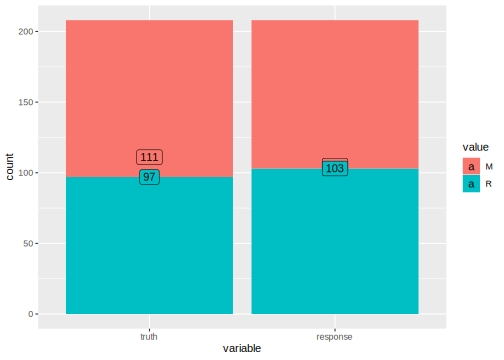
\includegraphics{mlr3book_files/figure-latex/02-basics-041-1} \end{center}

\begin{Shaded}
\begin{Highlighting}[]
\KeywordTok{autoplot}\NormalTok{(prediction, }\DataTypeTok{type =} \StringTok{"roc"}\NormalTok{)}
\end{Highlighting}
\end{Shaded}

\begin{center}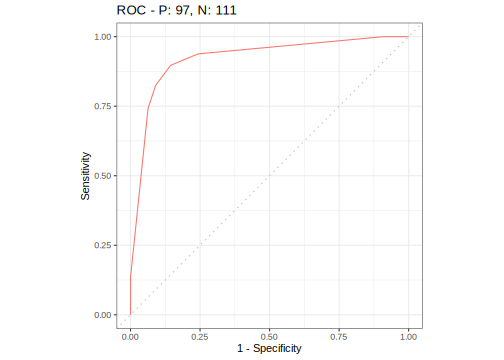
\includegraphics{mlr3book_files/figure-latex/02-basics-041-2} \end{center}

\begin{Shaded}
\begin{Highlighting}[]
\KeywordTok{library}\NormalTok{(mlr3viz)}
\KeywordTok{library}\NormalTok{(mlr3learners)}
\KeywordTok{local}\NormalTok{(\{}
  \CommentTok{# we do this locally to not overwrite the objects from}
  \CommentTok{# previous chunks}
\NormalTok{  task =}\StringTok{ }\KeywordTok{tsk}\NormalTok{(}\StringTok{"mtcars"}\NormalTok{)}
\NormalTok{  learner =}\StringTok{ }\KeywordTok{lrn}\NormalTok{(}\StringTok{"regr.lm"}\NormalTok{)}
\NormalTok{  learner}\OperatorTok{$}\KeywordTok{train}\NormalTok{(task)}
\NormalTok{  prediction =}\StringTok{ }\NormalTok{learner}\OperatorTok{$}\KeywordTok{predict}\NormalTok{(task)}
  \KeywordTok{autoplot}\NormalTok{(prediction)}
\NormalTok{\})}
\end{Highlighting}
\end{Shaded}

\begin{center}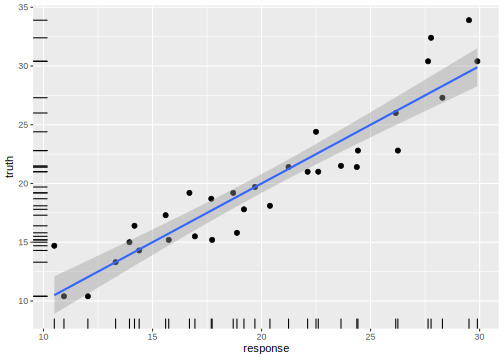
\includegraphics{mlr3book_files/figure-latex/02-basics-042-1} \end{center}

\hypertarget{measure}{%
\subsection{Performance assessment}\label{measure}}

The last step of an modeling is usually the performance assessment.
The quality of the predictions of a model in \href{https://mlr3.mlr-org.com}{mlr3} can be assessed with respect to a number of different performance measures.
At the performance assessment we choose a specific performance measure to quantify the predictions.
This is done by comparing the predicted labels with the true labels.
Predefined available measures are stored in \texttt{mlr\_measures} (with convenience getter \texttt{msr()}):

\begin{Shaded}
\begin{Highlighting}[]
\NormalTok{mlr_measures}
\NormalTok{## <DictionaryMeasure> with 72 stored values}
\NormalTok{## Keys: classif.acc, classif.auc, classif.bacc,}
\NormalTok{##   classif.ce, classif.costs, classif.dor,}
\NormalTok{##   classif.fbeta, classif.fdr, classif.fn,}
\NormalTok{##   classif.fnr, classif.fomr, classif.fp,}
\NormalTok{##   classif.fpr, classif.logloss, classif.mcc,}
\NormalTok{##   classif.npv, classif.ppv, classif.precision,}
\NormalTok{##   classif.recall, classif.sensitivity,}
\NormalTok{##   classif.specificity, classif.tn, classif.tnr,}
\NormalTok{##   classif.tp, classif.tpr, debug, oob_error,}
\NormalTok{##   regr.bias, regr.ktau, regr.mae, regr.mape,}
\NormalTok{##   regr.maxae, regr.medae, regr.medse, regr.mse,}
\NormalTok{##   regr.msle, regr.pbias, regr.rae, regr.rmse,}
\NormalTok{##   regr.rmsle, regr.rrse, regr.rse, regr.rsq,}
\NormalTok{##   regr.sae, regr.smape, regr.srho, regr.sse,}
\NormalTok{##   selected_features, surv.beggC,}
\NormalTok{##   surv.chamblessAUC, surv.gonenC, surv.graf,}
\NormalTok{##   surv.grafSE, surv.harrellC, surv.hungAUC,}
\NormalTok{##   surv.intlogloss, surv.intloglossSE,}
\NormalTok{##   surv.logloss, surv.loglossSE, surv.nagelkR2,}
\NormalTok{##   surv.oquigleyR2, surv.songAUC, surv.songTNR,}
\NormalTok{##   surv.songTPR, surv.unoAUC, surv.unoC,}
\NormalTok{##   surv.unoTNR, surv.unoTPR, surv.xuR2, time_both,}
\NormalTok{##   time_predict, time_train}
\end{Highlighting}
\end{Shaded}

We select the accuracy (\texttt{mlr\_measures\_classif.acc",\ text\ =\ "classif.acc}) and call the method \texttt{\$score()} of the \texttt{Prediction} object.

\begin{Shaded}
\begin{Highlighting}[]
\NormalTok{measure =}\StringTok{ }\KeywordTok{msr}\NormalTok{(}\StringTok{"classif.acc"}\NormalTok{)}
\NormalTok{prediction}\OperatorTok{$}\KeywordTok{score}\NormalTok{(measure)}
\NormalTok{## classif.acc }
\NormalTok{##       0.875}
\end{Highlighting}
\end{Shaded}

Note that, if no measure is specified, classification defaults to classification error (\texttt{mlr\_measures\_classif.ce",\ text\ =\ "classif.ce}) and regression defaults to the mean squared error (\texttt{mlr\_measures\_regr.mse",\ text\ =\ "regr.mse}).

\hypertarget{resampling}{%
\section{Resampling}\label{resampling}}

Resampling strategies are usually used to assess the performance of a learning algorithm.
\href{https://mlr3.mlr-org.com}{mlr3} entails 6 predefined \protect\hyperlink{resampling}{resampling} strategies:
Cross-validation, Leave-one-out cross validation, Repeated cross-validation, Out-of-bag bootstrap and other variants (e.g.~b632), Monte-Carlo cross-validation and Holdout.
The following sections provide guidance on how to set and select a resampling strategy and how to subsequently instantiate the resampling process.

Below you can find a graphical illustration of the resampling process:

\begin{center}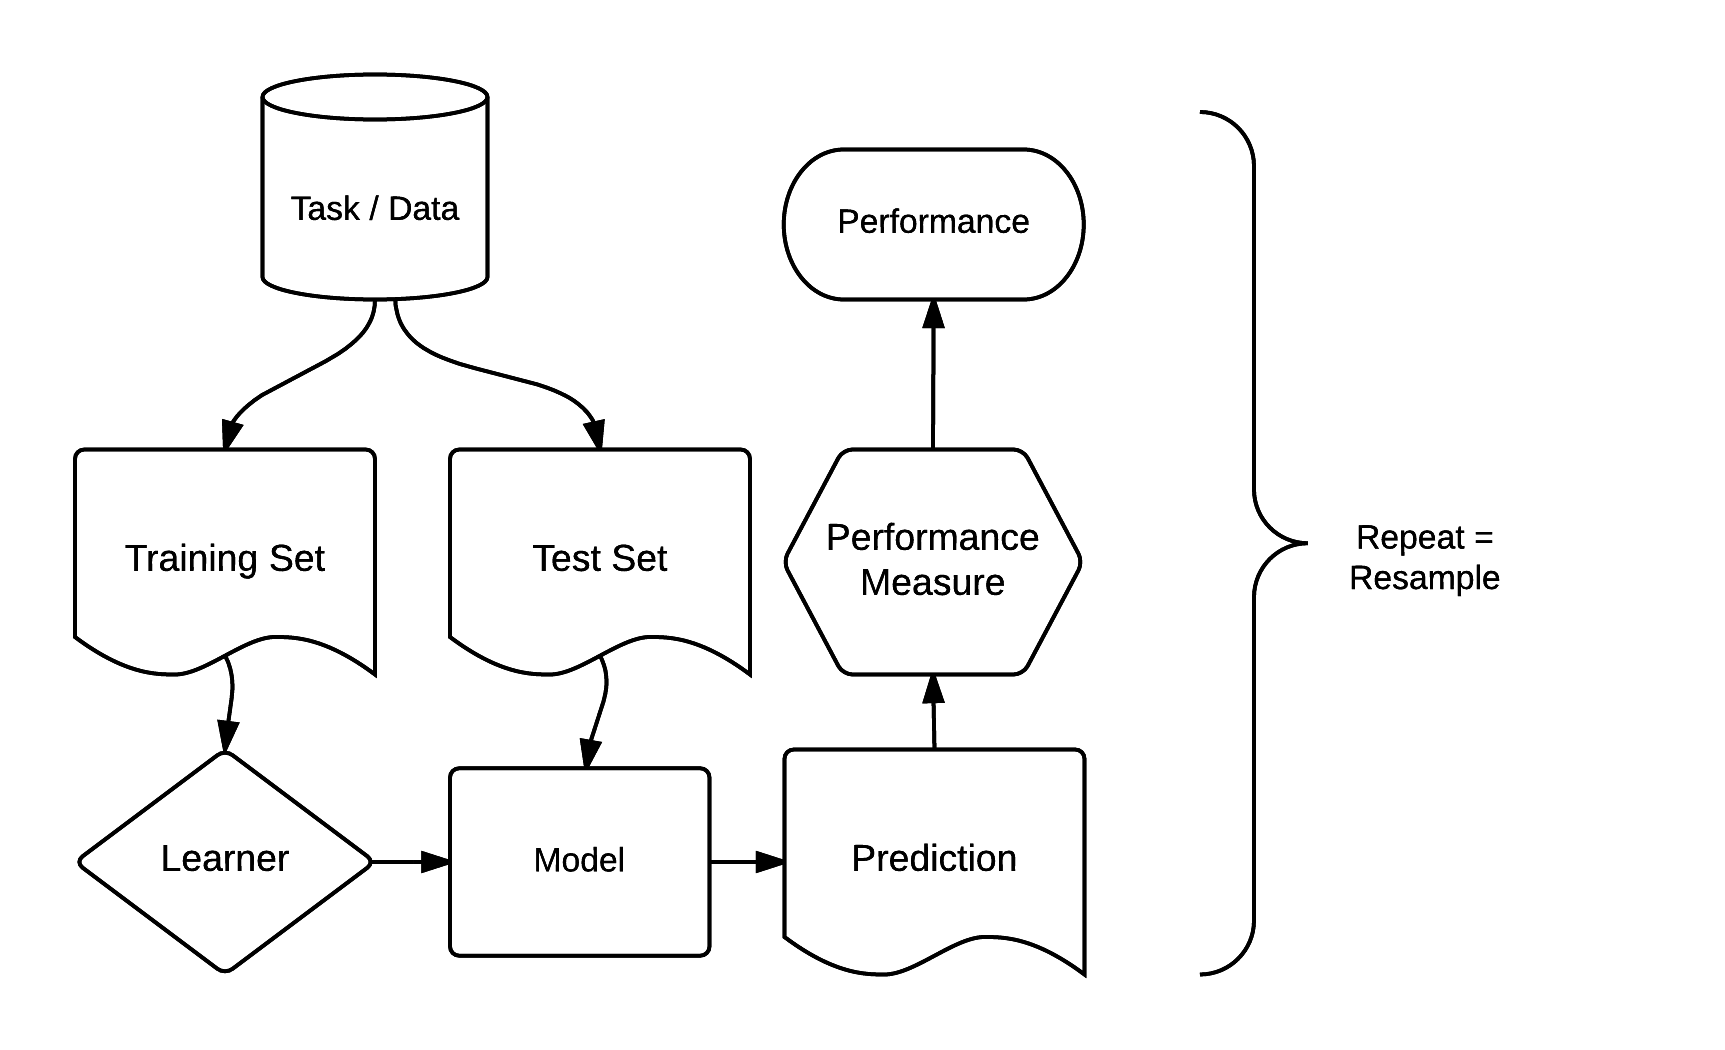
\includegraphics{images/ml_abstraction} \end{center}

\hypertarget{resamp-settings}{%
\subsection{Settings}\label{resamp-settings}}

In this example we use the \emph{iris} task and a simple classification tree (package \texttt{rpart}).

\begin{Shaded}
\begin{Highlighting}[]
\NormalTok{task =}\StringTok{ }\KeywordTok{tsk}\NormalTok{(}\StringTok{"iris"}\NormalTok{)}
\NormalTok{learner =}\StringTok{ }\KeywordTok{lrn}\NormalTok{(}\StringTok{"classif.rpart"}\NormalTok{)}
\end{Highlighting}
\end{Shaded}

When performing resampling with a dataset, we first need to define which approach should be used.
The resampling strategies of \emph{mlr3} can be queried using the \texttt{.\$keys()} method of the \texttt{mlr\_resamplings} dictionary.

\begin{Shaded}
\begin{Highlighting}[]
\NormalTok{mlr_resamplings}
\NormalTok{## <DictionaryResampling> with 6 stored values}
\NormalTok{## Keys: bootstrap, custom, cv, holdout,}
\NormalTok{##   repeated_cv, subsampling}
\end{Highlighting}
\end{Shaded}

Additional resampling methods for special use cases will be available via extension packages, such as \texttt{mlr-org/mlr3spatiotemporal} for spatial data (still in development).

The model fit conducted in the \protect\hyperlink{train-predict}{train/predict/score} chapter is equivalent to a ``holdout'', so let's consider this one first.
Again, we can retrieve elements from the dictionary \texttt{mlr\_resamplings} via \texttt{\$get()} or with a convenience function (\texttt{rsmp()}):

\begin{Shaded}
\begin{Highlighting}[]
\NormalTok{resampling =}\StringTok{ }\KeywordTok{rsmp}\NormalTok{(}\StringTok{"holdout"}\NormalTok{)}
\KeywordTok{print}\NormalTok{(resampling)}
\NormalTok{## <ResamplingHoldout> with 1 iterations}
\NormalTok{## * Instantiated: FALSE}
\NormalTok{## * Parameters: ratio=0.6667}
\end{Highlighting}
\end{Shaded}

Note that the \texttt{Instantiated} field is set to \texttt{FALSE}.
This means we did not actually apply the strategy on a dataset yet, but just performed a dry-run.
Applying the strategy on a dataset is done in section next \protect\hyperlink{instantiation}{Instantiation}.

By default we get a .66/.33 split of the data.
There are two ways in which the ratio can be changed:

\begin{enumerate}
\def\labelenumi{\arabic{enumi}.}
\tightlist
\item
  Overwriting the slot in \texttt{.\$param\_set\$values} using a named list:
\end{enumerate}

\begin{Shaded}
\begin{Highlighting}[]
\NormalTok{resampling}\OperatorTok{$}\NormalTok{param_set}\OperatorTok{$}\NormalTok{values =}\StringTok{ }\KeywordTok{list}\NormalTok{(}\DataTypeTok{ratio =} \FloatTok{0.8}\NormalTok{)}
\end{Highlighting}
\end{Shaded}

\begin{enumerate}
\def\labelenumi{\arabic{enumi}.}
\setcounter{enumi}{1}
\tightlist
\item
  Specifying the resampling parameters directly during construction:
\end{enumerate}

\begin{Shaded}
\begin{Highlighting}[]
\KeywordTok{rsmp}\NormalTok{(}\StringTok{"holdout"}\NormalTok{, }\DataTypeTok{ratio =} \FloatTok{0.8}\NormalTok{)}
\NormalTok{## <ResamplingHoldout> with 1 iterations}
\NormalTok{## * Instantiated: FALSE}
\NormalTok{## * Parameters: ratio=0.8}
\end{Highlighting}
\end{Shaded}

\hypertarget{resampling-inst}{%
\subsection{Instantiation}\label{resampling-inst}}

So far we just set the stage and selected the resampling strategy.
To actually perform the splitting, the resampling needs a \texttt{Task}.
By calling the method \texttt{instantiate()}, splits into training and test set are calculated and stored in the \texttt{Resampling} object:

\begin{Shaded}
\begin{Highlighting}[]
\NormalTok{resampling =}\StringTok{ }\KeywordTok{rsmp}\NormalTok{(}\StringTok{"cv"}\NormalTok{, }\DataTypeTok{folds =}\NormalTok{ 3L)}
\NormalTok{resampling}\OperatorTok{$}\KeywordTok{instantiate}\NormalTok{(task)}
\NormalTok{resampling}\OperatorTok{$}\NormalTok{iters}
\NormalTok{## [1] 3}
\KeywordTok{str}\NormalTok{(resampling}\OperatorTok{$}\KeywordTok{train_set}\NormalTok{(}\DecValTok{1}\NormalTok{))}
\NormalTok{##  int [1:100] 1 7 9 11 12 15 16 17 18 19 ...}
\KeywordTok{str}\NormalTok{(resampling}\OperatorTok{$}\KeywordTok{test_set}\NormalTok{(}\DecValTok{1}\NormalTok{))}
\NormalTok{##  int [1:50] 3 10 20 21 26 27 28 29 39 43 ...}
\end{Highlighting}
\end{Shaded}

\hypertarget{resampling-exec}{%
\subsection{Execution}\label{resampling-exec}}

With a \texttt{Task}, a \texttt{Learner} and \texttt{Resampling} object we can call \texttt{resample()} and create a \texttt{ResampleResult} object.

Before we go into more detail, let's change the resampling to a ``3-fold cross-validation'' to better illustrate what operations are possible with a \texttt{ResampleResult}.
Additionally, we tell \texttt{resample()} to keep the fitted models via the flag \texttt{store\_models}:

\begin{Shaded}
\begin{Highlighting}[]
\NormalTok{task =}\StringTok{ }\KeywordTok{tsk}\NormalTok{(}\StringTok{"pima"}\NormalTok{)}
\NormalTok{learner =}\StringTok{ }\KeywordTok{lrn}\NormalTok{(}\StringTok{"classif.rpart"}\NormalTok{, }\DataTypeTok{maxdepth =} \DecValTok{3}\NormalTok{, }\DataTypeTok{predict_type =} \StringTok{"prob"}\NormalTok{)}
\NormalTok{resampling =}\StringTok{ }\KeywordTok{rsmp}\NormalTok{(}\StringTok{"cv"}\NormalTok{, }\DataTypeTok{folds =}\NormalTok{ 3L)}

\NormalTok{rr =}\StringTok{ }\KeywordTok{resample}\NormalTok{(task, learner, resampling, }\DataTypeTok{store_models =} \OtherTok{TRUE}\NormalTok{)}
\KeywordTok{print}\NormalTok{(rr)}
\NormalTok{## <ResampleResult> of 3 iterations}
\NormalTok{## * Task: pima}
\NormalTok{## * Learner: classif.rpart}
\NormalTok{## * Warnings: 0 in 0 iterations}
\NormalTok{## * Errors: 0 in 0 iterations}
\end{Highlighting}
\end{Shaded}

The following operations are supported with \texttt{ResampleResult} objects:

\begin{itemize}
\item
  Calculate the average performance:

\begin{Shaded}
\begin{Highlighting}[]
\NormalTok{rr}\OperatorTok{$}\KeywordTok{aggregate}\NormalTok{(}\KeywordTok{msr}\NormalTok{(}\StringTok{"classif.ce"}\NormalTok{))}
\NormalTok{## classif.ce }
\NormalTok{##     0.2617}
\end{Highlighting}
\end{Shaded}
\item
  Extract the performance for the individual resampling iterations:

\begin{Shaded}
\begin{Highlighting}[]
\NormalTok{rr}\OperatorTok{$}\KeywordTok{score}\NormalTok{(}\KeywordTok{msr}\NormalTok{(}\StringTok{"classif.ce"}\NormalTok{))}
\NormalTok{##             task task_id               learner}
\NormalTok{## 1: <TaskClassif>    pima <LearnerClassifRpart>}
\NormalTok{## 2: <TaskClassif>    pima <LearnerClassifRpart>}
\NormalTok{## 3: <TaskClassif>    pima <LearnerClassifRpart>}
\NormalTok{##       learner_id     resampling resampling_id iteration}
\NormalTok{## 1: classif.rpart <ResamplingCV>            cv         1}
\NormalTok{## 2: classif.rpart <ResamplingCV>            cv         2}
\NormalTok{## 3: classif.rpart <ResamplingCV>            cv         3}
\NormalTok{##    prediction classif.ce}
\NormalTok{## 1:     <list>     0.2539}
\NormalTok{## 2:     <list>     0.2734}
\NormalTok{## 3:     <list>     0.2578}
\end{Highlighting}
\end{Shaded}
\item
  Check for warnings or errors:

\begin{Shaded}
\begin{Highlighting}[]
\NormalTok{rr}\OperatorTok{$}\NormalTok{warnings}
\NormalTok{## Empty data.table (0 rows and 2 cols): iteration,msg}
\NormalTok{rr}\OperatorTok{$}\NormalTok{errors}
\NormalTok{## Empty data.table (0 rows and 2 cols): iteration,msg}
\end{Highlighting}
\end{Shaded}
\item
  Extract and inspect the resampling splits:

\begin{Shaded}
\begin{Highlighting}[]
\NormalTok{rr}\OperatorTok{$}\NormalTok{resampling}
\NormalTok{## <ResamplingCV> with 3 iterations}
\NormalTok{## * Instantiated: TRUE}
\NormalTok{## * Parameters: folds=3}
\NormalTok{rr}\OperatorTok{$}\NormalTok{resampling}\OperatorTok{$}\NormalTok{iters}
\NormalTok{## [1] 3}
\KeywordTok{str}\NormalTok{(rr}\OperatorTok{$}\NormalTok{resampling}\OperatorTok{$}\KeywordTok{test_set}\NormalTok{(}\DecValTok{1}\NormalTok{))}
\NormalTok{##  int [1:256] 2 6 15 16 17 19 24 27 39 42 ...}
\KeywordTok{str}\NormalTok{(rr}\OperatorTok{$}\NormalTok{resampling}\OperatorTok{$}\KeywordTok{train_set}\NormalTok{(}\DecValTok{1}\NormalTok{))}
\NormalTok{##  int [1:512] 1 3 4 5 7 10 12 18 23 25 ...}
\end{Highlighting}
\end{Shaded}
\item
  Retrieve the \protect\hyperlink{learners}{learner} of a specific iteration and inspect it:

\begin{Shaded}
\begin{Highlighting}[]
\NormalTok{lrn =}\StringTok{ }\NormalTok{rr}\OperatorTok{$}\NormalTok{learners[[}\DecValTok{1}\NormalTok{]]}
\NormalTok{lrn}\OperatorTok{$}\NormalTok{model}
\NormalTok{## n= 512 }
\NormalTok{## }
\NormalTok{## node), split, n, loss, yval, (yprob)}
\NormalTok{##       * denotes terminal node}
\NormalTok{## }
\NormalTok{##  1) root 512 175 neg (0.6582 0.3418)  }
\NormalTok{##    2) glucose< 127.5 331  63 neg (0.8097 0.1903) *}
\NormalTok{##    3) glucose>=127.5 181  69 pos (0.3812 0.6188)  }
\NormalTok{##      6) mass< 29.95 49  13 neg (0.7347 0.2653)  }
\NormalTok{##       12) glucose< 154.5 35   5 neg (0.8571 0.1429) *}
\NormalTok{##       13) glucose>=154.5 14   6 pos (0.4286 0.5714) *}
\NormalTok{##      7) mass>=29.95 132  33 pos (0.2500 0.7500) *}
\end{Highlighting}
\end{Shaded}
\item
  Extract the predictions:

\begin{Shaded}
\begin{Highlighting}[]
\NormalTok{rr}\OperatorTok{$}\KeywordTok{prediction}\NormalTok{()  }\CommentTok{# all predictions merged into a single Prediction}
\NormalTok{## <PredictionClassif> for 768 observations:}
\NormalTok{##     row_id truth response prob.pos prob.neg}
\NormalTok{##          2   neg      neg   0.1903   0.8097}
\NormalTok{##          6   neg      neg   0.1903   0.8097}
\NormalTok{##         15   pos      pos   0.5714   0.4286}
\NormalTok{## ---                                        }
\NormalTok{##        762   pos      pos   0.8889   0.1111}
\NormalTok{##        763   neg      neg   0.1763   0.8237}
\NormalTok{##        767   pos      pos   0.5840   0.4160}
\NormalTok{rr}\OperatorTok{$}\KeywordTok{predictions}\NormalTok{()[[}\DecValTok{1}\NormalTok{]]  }\CommentTok{# prediction of first resampling iteration}
\NormalTok{## <PredictionClassif> for 256 observations:}
\NormalTok{##     row_id truth response prob.pos prob.neg}
\NormalTok{##          2   neg      neg   0.1903   0.8097}
\NormalTok{##          6   neg      neg   0.1903   0.8097}
\NormalTok{##         15   pos      pos   0.5714   0.4286}
\NormalTok{## ---                                        }
\NormalTok{##        758   pos      neg   0.1903   0.8097}
\NormalTok{##        759   neg      neg   0.1903   0.8097}
\NormalTok{##        765   neg      neg   0.1903   0.8097}
\end{Highlighting}
\end{Shaded}
\end{itemize}

Note that if you want to compare multiple \protect\hyperlink{learners}{learners}, you should ensure to that each learner operates on the same resampling instance by manually instantiating beforehand.
This reduces the variance of the performance estimation.

If your aim is to compare different \texttt{Task}, \texttt{Learner} or \texttt{Resampling}, you are better off using the \texttt{benchmark()} function, covered in the \protect\hyperlink{benchmarking}{next section}.
It is basically a wrapper around \texttt{resample()} simplifying the handling of multiple settings.
If you discover this only after you've run multiple \texttt{resample()} calls, don't worry.
You can combine multiple \texttt{ResampleResult} objects into a \texttt{BenchmarkResult} (also explained in the \protect\hyperlink{benchmarking}{next section}).

\hypertarget{resamp-custom}{%
\subsection{Custom resampling}\label{resamp-custom}}

Sometimes it is necessary to perform resampling with custom splits.
If you want to do that because you are coming from a specific modeling field, first take a look at the \emph{mlr3} extension packages.
It is important to make sure that your custom resampling method has not been implemented already.

If your custom resampling method is widely used in your field, feel welcome to integrate it into one of the existing \emph{mlr3} extension packages.
You could also create your own extension package.

A manual resampling instance can be created using the \texttt{"custom"} template.

\begin{Shaded}
\begin{Highlighting}[]
\NormalTok{resampling =}\StringTok{ }\KeywordTok{rsmp}\NormalTok{(}\StringTok{"custom"}\NormalTok{)}
\NormalTok{resampling}\OperatorTok{$}\KeywordTok{instantiate}\NormalTok{(task, }\DataTypeTok{train =} \KeywordTok{list}\NormalTok{(}\KeywordTok{c}\NormalTok{(}\DecValTok{1}\OperatorTok{:}\DecValTok{10}\NormalTok{, }\DecValTok{51}\OperatorTok{:}\DecValTok{60}\NormalTok{, }
  \DecValTok{101}\OperatorTok{:}\DecValTok{110}\NormalTok{)), }\DataTypeTok{test =} \KeywordTok{list}\NormalTok{(}\KeywordTok{c}\NormalTok{(}\DecValTok{11}\OperatorTok{:}\DecValTok{20}\NormalTok{, }\DecValTok{61}\OperatorTok{:}\DecValTok{70}\NormalTok{, }\DecValTok{111}\OperatorTok{:}\DecValTok{120}\NormalTok{)))}
\NormalTok{resampling}\OperatorTok{$}\NormalTok{iters}
\NormalTok{## [1] 1}
\NormalTok{resampling}\OperatorTok{$}\KeywordTok{train_set}\NormalTok{(}\DecValTok{1}\NormalTok{)}
\NormalTok{##  [1]   1   2   3   4   5   6   7   8   9  10  51  52  53}
\NormalTok{## [14]  54  55  56  57  58  59  60 101 102 103 104 105 106}
\NormalTok{## [27] 107 108 109 110}
\NormalTok{resampling}\OperatorTok{$}\KeywordTok{test_set}\NormalTok{(}\DecValTok{1}\NormalTok{)}
\NormalTok{##  [1]  11  12  13  14  15  16  17  18  19  20  61  62  63}
\NormalTok{## [14]  64  65  66  67  68  69  70 111 112 113 114 115 116}
\NormalTok{## [27] 117 118 119 120}
\end{Highlighting}
\end{Shaded}

\hypertarget{autoplot-resampleresult}{%
\subsection{Plotting Resample Results}\label{autoplot-resampleresult}}

Again, \href{https://mlr3viz.mlr-org.com}{mlr3viz} provides a \texttt{ggplot2::autoplot()",\ text\ =\ "autoplot()} method.

\begin{Shaded}
\begin{Highlighting}[]
\KeywordTok{library}\NormalTok{(mlr3viz)}

\KeywordTok{autoplot}\NormalTok{(rr)}
\end{Highlighting}
\end{Shaded}

\begin{center}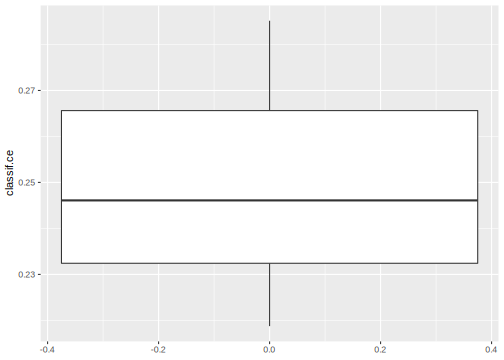
\includegraphics{mlr3book_files/figure-latex/02-basics-060-1} \end{center}

\begin{Shaded}
\begin{Highlighting}[]
\KeywordTok{autoplot}\NormalTok{(rr, }\DataTypeTok{type =} \StringTok{"roc"}\NormalTok{)}
\end{Highlighting}
\end{Shaded}

\begin{center}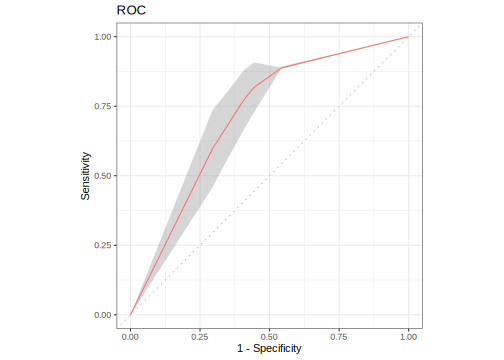
\includegraphics{mlr3book_files/figure-latex/02-basics-060-2} \end{center}

All available plot types are listed on the manual page of \texttt{autoplot.ResampleResult()}.

\hypertarget{benchmarking}{%
\section{Benchmarking}\label{benchmarking}}

Comparing the performance of different learners on multiple tasks and/or different resampling schemes is a recurrent task.
This operation is usually referred to as ``benchmarking'' in the field of machine-learning.
The \href{https://mlr3.mlr-org.com}{mlr3} package offers the \texttt{benchmark()} function for convenience.

\hypertarget{bm-design}{%
\subsection{Design Creation}\label{bm-design}}

In \emph{mlr3} we require you to supply a ``design'' of your benchmark experiment.
By ``design'' we essentially mean the matrix of settings you want to execute.
A ``design'' consists of \texttt{Task}, \texttt{Learner} and \texttt{Resampling}.

Here, we call \texttt{benchmark()} to perform a single holdout split on a single task and two learners.
We use the \texttt{benchmark\_grid()} function to create an exhaustive design and properly instantiate the resampling:

\begin{Shaded}
\begin{Highlighting}[]
\KeywordTok{library}\NormalTok{(data.table)}
\NormalTok{design =}\StringTok{ }\KeywordTok{benchmark_grid}\NormalTok{(}\DataTypeTok{tasks =} \KeywordTok{tsk}\NormalTok{(}\StringTok{"iris"}\NormalTok{), }\DataTypeTok{learners =} \KeywordTok{list}\NormalTok{(}\KeywordTok{lrn}\NormalTok{(}\StringTok{"classif.rpart"}\NormalTok{), }
  \KeywordTok{lrn}\NormalTok{(}\StringTok{"classif.featureless"}\NormalTok{)), }\DataTypeTok{resamplings =} \KeywordTok{rsmp}\NormalTok{(}\StringTok{"holdout"}\NormalTok{))}
\KeywordTok{print}\NormalTok{(design)}
\NormalTok{##             task                     learner}
\NormalTok{## 1: <TaskClassif>       <LearnerClassifRpart>}
\NormalTok{## 2: <TaskClassif> <LearnerClassifFeatureless>}
\NormalTok{##             resampling}
\NormalTok{## 1: <ResamplingHoldout>}
\NormalTok{## 2: <ResamplingHoldout>}
\NormalTok{bmr =}\StringTok{ }\KeywordTok{benchmark}\NormalTok{(design)}
\end{Highlighting}
\end{Shaded}

Note that the holdout splits have been automatically instantiated for each row of the design.
As a result, the \texttt{rpart} learner used a different training set than the \texttt{featureless} learner.
However, for comparison of learners you usually want the learners to see the same splits into train and test sets.
To overcome this issue, the resampling strategy needs to be \protect\hyperlink{resampling-inst}{\textbf{manually instantiated}} before creating the design.

The interface of \texttt{benchmark()} allows for full flexibility.
Irrespective, the creation of such design tables can be tedious.
Therefore, \href{https://mlr3.mlr-org.com}{mlr3} provides a convenience function to quickly generate design tables and instantiate resampling strategies in an exhaustive grid fashion: \texttt{benchmark\_grid()}.

\begin{Shaded}
\begin{Highlighting}[]
\CommentTok{# get some example tasks}
\NormalTok{tasks =}\StringTok{ }\KeywordTok{lapply}\NormalTok{(}\KeywordTok{c}\NormalTok{(}\StringTok{"german_credit"}\NormalTok{, }\StringTok{"sonar"}\NormalTok{), tsk)}

\CommentTok{# get some learners and for all learners ...  * predict}
\CommentTok{# probabilities * predict also on the training set}
\KeywordTok{library}\NormalTok{(mlr3learners)}
\NormalTok{learners =}\StringTok{ }\KeywordTok{c}\NormalTok{(}\StringTok{"classif.featureless"}\NormalTok{, }\StringTok{"classif.rpart"}\NormalTok{, }\StringTok{"classif.ranger"}\NormalTok{, }
  \StringTok{"classif.kknn"}\NormalTok{)}
\NormalTok{learners =}\StringTok{ }\KeywordTok{lapply}\NormalTok{(learners, lrn, }\DataTypeTok{predict_type =} \StringTok{"prob"}\NormalTok{, }\DataTypeTok{predict_sets =} \KeywordTok{c}\NormalTok{(}\StringTok{"train"}\NormalTok{, }
  \StringTok{"test"}\NormalTok{))}

\CommentTok{# compare via 3-fold cross validation}
\NormalTok{resamplings =}\StringTok{ }\KeywordTok{rsmp}\NormalTok{(}\StringTok{"cv"}\NormalTok{, }\DataTypeTok{folds =} \DecValTok{3}\NormalTok{)}

\CommentTok{# create a BenchmarkDesign object}
\NormalTok{design =}\StringTok{ }\KeywordTok{benchmark_grid}\NormalTok{(tasks, learners, resamplings)}
\KeywordTok{print}\NormalTok{(design)}
\NormalTok{##             task                     learner}
\NormalTok{## 1: <TaskClassif> <LearnerClassifFeatureless>}
\NormalTok{## 2: <TaskClassif>       <LearnerClassifRpart>}
\NormalTok{## 3: <TaskClassif>      <LearnerClassifRanger>}
\NormalTok{## 4: <TaskClassif>        <LearnerClassifKKNN>}
\NormalTok{## 5: <TaskClassif> <LearnerClassifFeatureless>}
\NormalTok{## 6: <TaskClassif>       <LearnerClassifRpart>}
\NormalTok{## 7: <TaskClassif>      <LearnerClassifRanger>}
\NormalTok{## 8: <TaskClassif>        <LearnerClassifKKNN>}
\NormalTok{##        resampling}
\NormalTok{## 1: <ResamplingCV>}
\NormalTok{## 2: <ResamplingCV>}
\NormalTok{## 3: <ResamplingCV>}
\NormalTok{## 4: <ResamplingCV>}
\NormalTok{## 5: <ResamplingCV>}
\NormalTok{## 6: <ResamplingCV>}
\NormalTok{## 7: <ResamplingCV>}
\NormalTok{## 8: <ResamplingCV>}
\end{Highlighting}
\end{Shaded}

\hypertarget{bm-exec}{%
\subsection{Execution and Aggregation of Results}\label{bm-exec}}

After the \protect\hyperlink{bm-design}{benchmark design} is ready, we can directly call \texttt{benchmark()}:

\begin{Shaded}
\begin{Highlighting}[]
\CommentTok{# execute the benchmark}
\NormalTok{bmr =}\StringTok{ }\KeywordTok{benchmark}\NormalTok{(design)}
\end{Highlighting}
\end{Shaded}

Note that we did not instantiate the resampling instance.
\texttt{benchmark\_grid()} took care of it for us:
Each resampling strategy is instantiated for each task during the construction of the exhaustive grid.

After the benchmark, one can calculate and aggregate the performance with \texttt{.\$aggregate()}:

\begin{Shaded}
\begin{Highlighting}[]
\CommentTok{# measures: * area under the curve (auc) on training *}
\CommentTok{# area under the curve (auc) on test}
\NormalTok{measures =}\StringTok{ }\KeywordTok{list}\NormalTok{(}\KeywordTok{msr}\NormalTok{(}\StringTok{"classif.auc"}\NormalTok{, }\DataTypeTok{id =} \StringTok{"auc_train"}\NormalTok{, }\DataTypeTok{predict_sets =} \StringTok{"train"}\NormalTok{), }
  \KeywordTok{msr}\NormalTok{(}\StringTok{"classif.auc"}\NormalTok{, }\DataTypeTok{id =} \StringTok{"auc_test"}\NormalTok{))}
\NormalTok{bmr}\OperatorTok{$}\KeywordTok{aggregate}\NormalTok{(measures)}
\NormalTok{##    nr  resample_result       task_id}
\NormalTok{## 1:  1 <ResampleResult> german_credit}
\NormalTok{## 2:  2 <ResampleResult> german_credit}
\NormalTok{## 3:  3 <ResampleResult> german_credit}
\NormalTok{## 4:  4 <ResampleResult> german_credit}
\NormalTok{## 5:  5 <ResampleResult>         sonar}
\NormalTok{## 6:  6 <ResampleResult>         sonar}
\NormalTok{## 7:  7 <ResampleResult>         sonar}
\NormalTok{## 8:  8 <ResampleResult>         sonar}
\NormalTok{##             learner_id resampling_id iters auc_train}
\NormalTok{## 1: classif.featureless            cv     3    0.5000}
\NormalTok{## 2:       classif.rpart            cv     3    0.8041}
\NormalTok{## 3:      classif.ranger            cv     3    0.9987}
\NormalTok{## 4:        classif.kknn            cv     3    0.9889}
\NormalTok{## 5: classif.featureless            cv     3    0.5000}
\NormalTok{## 6:       classif.rpart            cv     3    0.9369}
\NormalTok{## 7:      classif.ranger            cv     3    1.0000}
\NormalTok{## 8:        classif.kknn            cv     3    0.9982}
\NormalTok{##    auc_test}
\NormalTok{## 1:   0.5000}
\NormalTok{## 2:   0.7200}
\NormalTok{## 3:   0.7948}
\NormalTok{## 4:   0.7179}
\NormalTok{## 5:   0.5000}
\NormalTok{## 6:   0.8001}
\NormalTok{## 7:   0.9004}
\NormalTok{## 8:   0.9194}
\end{Highlighting}
\end{Shaded}

Subsequently, we can aggregate the results further.
For example, we might be interested which learner performed best over all tasks simultaneously.
Simply aggregating the performances with the mean is usually not statistically sound.
Instead, we calculate the rank statistic for each learner grouped by task.
Then the calculated ranks grouped by learner are aggregated.
Since the AUC needs to be maximized, we multiply with \(-1\) so that the best learner gets a rank of 1.

\begin{Shaded}
\begin{Highlighting}[]
\NormalTok{tab =}\StringTok{ }\NormalTok{bmr}\OperatorTok{$}\KeywordTok{aggregate}\NormalTok{(measures)}
\NormalTok{ranks =}\StringTok{ }\NormalTok{tab[, .(learner_id, }\DataTypeTok{rank_train =} \KeywordTok{rank}\NormalTok{(}\OperatorTok{-}\NormalTok{auc_train), }
  \DataTypeTok{rank_test =} \KeywordTok{rank}\NormalTok{(}\OperatorTok{-}\NormalTok{auc_test)), by =}\StringTok{ }\NormalTok{task_id]}
\KeywordTok{print}\NormalTok{(ranks)}
\NormalTok{##          task_id          learner_id rank_train}
\NormalTok{## 1: german_credit classif.featureless          4}
\NormalTok{## 2: german_credit       classif.rpart          3}
\NormalTok{## 3: german_credit      classif.ranger          1}
\NormalTok{## 4: german_credit        classif.kknn          2}
\NormalTok{## 5:         sonar classif.featureless          4}
\NormalTok{## 6:         sonar       classif.rpart          3}
\NormalTok{## 7:         sonar      classif.ranger          1}
\NormalTok{## 8:         sonar        classif.kknn          2}
\NormalTok{##    rank_test}
\NormalTok{## 1:         4}
\NormalTok{## 2:         2}
\NormalTok{## 3:         1}
\NormalTok{## 4:         3}
\NormalTok{## 5:         4}
\NormalTok{## 6:         3}
\NormalTok{## 7:         2}
\NormalTok{## 8:         1}

\NormalTok{ranks[, .(}\DataTypeTok{mrank_train =} \KeywordTok{mean}\NormalTok{(rank_train), }\DataTypeTok{mrank_test =} \KeywordTok{mean}\NormalTok{(rank_test)), }
\NormalTok{  by =}\StringTok{ }\NormalTok{learner_id][}\KeywordTok{order}\NormalTok{(mrank_test)]}
\NormalTok{##             learner_id mrank_train mrank_test}
\NormalTok{## 1:      classif.ranger           1        1.5}
\NormalTok{## 2:        classif.kknn           2        2.0}
\NormalTok{## 3:       classif.rpart           3        2.5}
\NormalTok{## 4: classif.featureless           4        4.0}
\end{Highlighting}
\end{Shaded}

Unsurprisingly, the featureless learner is outperformed.

\hypertarget{autoplot-benchmarkresult}{%
\subsection{Plotting Benchmark Results}\label{autoplot-benchmarkresult}}

Analogously to plotting \protect\hyperlink{autoplot-task}{tasks}, \protect\hyperlink{autoplot-prediction}{predictions} or \protect\hyperlink{autoplot-resampleresult}{resample results}, \href{https://mlr3viz.mlr-org.com}{mlr3viz} also provides a \texttt{ggplot2::autoplot()",\ text\ =\ "autoplot()} method for benchmark results.

\begin{Shaded}
\begin{Highlighting}[]
\KeywordTok{library}\NormalTok{(mlr3viz)}
\KeywordTok{library}\NormalTok{(ggplot2)}

\KeywordTok{autoplot}\NormalTok{(bmr) }\OperatorTok{+}\StringTok{ }\KeywordTok{theme}\NormalTok{(}\DataTypeTok{axis.text.x =} \KeywordTok{element_text}\NormalTok{(}\DataTypeTok{angle =} \DecValTok{45}\NormalTok{, }
  \DataTypeTok{hjust =} \DecValTok{1}\NormalTok{))}
\end{Highlighting}
\end{Shaded}

\begin{center}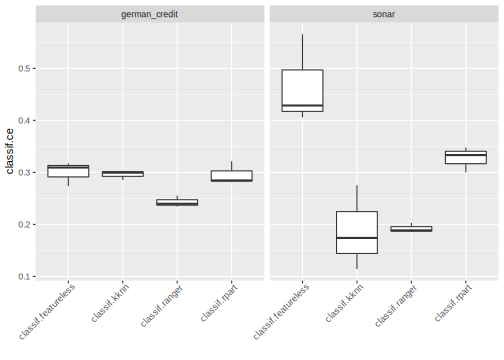
\includegraphics{mlr3book_files/figure-latex/02-basics-066-1} \end{center}

We can also plot ROC curves.
To do so, we first need to filter the \texttt{BenchmarkResult} to only contain a single \texttt{Task}:

\begin{Shaded}
\begin{Highlighting}[]
\KeywordTok{autoplot}\NormalTok{(bmr}\OperatorTok{$}\KeywordTok{clone}\NormalTok{()}\OperatorTok{$}\KeywordTok{filter}\NormalTok{(}\DataTypeTok{task_id =} \StringTok{"german_credit"}\NormalTok{), }\DataTypeTok{type =} \StringTok{"roc"}\NormalTok{)}
\end{Highlighting}
\end{Shaded}

\begin{center}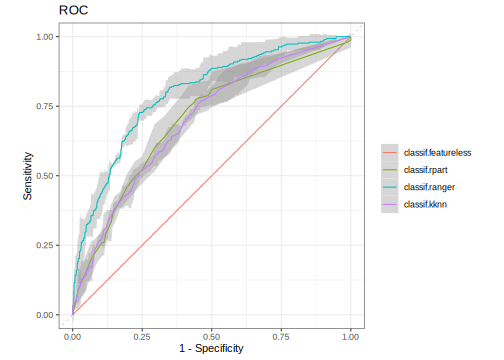
\includegraphics{mlr3book_files/figure-latex/02-basics-067-1} \end{center}

All available types are listed on the manual page of \texttt{autoplot.BenchmarkResult()}.

\hypertarget{bm-resamp}{%
\subsection{Extracting ResampleResults}\label{bm-resamp}}

A \texttt{BenchmarkResult} object is essentially a collection of multiple \texttt{ResampleResult} objects.
As these are stored in a column of the aggregated \texttt{data.table()}, we can easily extract them:

\begin{Shaded}
\begin{Highlighting}[]
\NormalTok{tab =}\StringTok{ }\NormalTok{bmr}\OperatorTok{$}\KeywordTok{aggregate}\NormalTok{(measures)}
\NormalTok{rr =}\StringTok{ }\NormalTok{tab[task_id }\OperatorTok{==}\StringTok{ "sonar"} \OperatorTok{&}\StringTok{ }\NormalTok{learner_id }\OperatorTok{==}\StringTok{ "classif.ranger"}\NormalTok{]}\OperatorTok{$}\NormalTok{resample_result[[}\DecValTok{1}\NormalTok{]]}
\KeywordTok{print}\NormalTok{(rr)}
\NormalTok{## <ResampleResult> of 3 iterations}
\NormalTok{## * Task: sonar}
\NormalTok{## * Learner: classif.ranger}
\NormalTok{## * Warnings: 0 in 0 iterations}
\NormalTok{## * Errors: 0 in 0 iterations}
\end{Highlighting}
\end{Shaded}

We can now investigate this resampling and even single resampling iterations using one of the approach shown in \protect\hyperlink{bm-exec}{the previous section}:

\begin{Shaded}
\begin{Highlighting}[]
\NormalTok{measure =}\StringTok{ }\KeywordTok{msr}\NormalTok{(}\StringTok{"classif.auc"}\NormalTok{)}
\NormalTok{rr}\OperatorTok{$}\KeywordTok{aggregate}\NormalTok{(measure)}
\NormalTok{## classif.auc }
\NormalTok{##      0.9004}

\CommentTok{# get the iteration with worst AUC}
\NormalTok{perf =}\StringTok{ }\NormalTok{rr}\OperatorTok{$}\KeywordTok{score}\NormalTok{(measure)}
\NormalTok{i =}\StringTok{ }\KeywordTok{which.min}\NormalTok{(perf}\OperatorTok{$}\NormalTok{classif.auc)}

\CommentTok{# get the corresponding learner and train set}
\KeywordTok{print}\NormalTok{(rr}\OperatorTok{$}\NormalTok{learners[[i]])}
\NormalTok{## <LearnerClassifRanger:classif.ranger>}
\NormalTok{## * Model: -}
\NormalTok{## * Parameters: list()}
\NormalTok{## * Packages: ranger}
\NormalTok{## * Predict Type: prob}
\NormalTok{## * Feature types: logical, integer, numeric,}
\NormalTok{##   character, factor, ordered}
\NormalTok{## * Properties: importance, multiclass, oob_error,}
\NormalTok{##   twoclass, weights}
\KeywordTok{head}\NormalTok{(rr}\OperatorTok{$}\NormalTok{resampling}\OperatorTok{$}\KeywordTok{train_set}\NormalTok{(i))}
\NormalTok{## [1]  7 12 13 14 17 18}
\end{Highlighting}
\end{Shaded}

\hypertarget{converting-and-merging-resampleresults}{%
\subsection{Converting and Merging ResampleResults}\label{converting-and-merging-resampleresults}}

It is also possible to cast a single \texttt{ResampleResult} to a \texttt{BenchmarkResult} using the converter \texttt{as\_benchmark\_result()}.

\begin{Shaded}
\begin{Highlighting}[]
\NormalTok{task =}\StringTok{ }\KeywordTok{tsk}\NormalTok{(}\StringTok{"iris"}\NormalTok{)}
\NormalTok{resampling =}\StringTok{ }\KeywordTok{rsmp}\NormalTok{(}\StringTok{"holdout"}\NormalTok{)}\OperatorTok{$}\KeywordTok{instantiate}\NormalTok{(task)}

\NormalTok{rr1 =}\StringTok{ }\KeywordTok{resample}\NormalTok{(task, }\KeywordTok{lrn}\NormalTok{(}\StringTok{"classif.rpart"}\NormalTok{), resampling)}
\NormalTok{rr2 =}\StringTok{ }\KeywordTok{resample}\NormalTok{(task, }\KeywordTok{lrn}\NormalTok{(}\StringTok{"classif.featureless"}\NormalTok{), resampling)}

\CommentTok{# Cast both ResampleResults to BenchmarkResults}
\NormalTok{bmr1 =}\StringTok{ }\KeywordTok{as_benchmark_result}\NormalTok{(rr1)}
\NormalTok{bmr2 =}\StringTok{ }\KeywordTok{as_benchmark_result}\NormalTok{(rr2)}

\CommentTok{# Merge 2nd BMR into the first BMR}
\NormalTok{bmr1}\OperatorTok{$}\KeywordTok{combine}\NormalTok{(bmr2)}

\NormalTok{bmr1}
\NormalTok{## <BenchmarkResult> of 2 rows with 2 resampling runs}
\NormalTok{##  nr task_id          learner_id resampling_id iters}
\NormalTok{##   1    iris       classif.rpart       holdout     1}
\NormalTok{##   2    iris classif.featureless       holdout     1}
\NormalTok{##  warnings errors}
\NormalTok{##         0      0}
\NormalTok{##         0      0}
\end{Highlighting}
\end{Shaded}

\hypertarget{binary}{%
\section{Binary classification}\label{binary}}

Classification problems with a target variable containing only two classes are called ``binary''.
For such binary target variables, you can specify the \emph{positive class} within the \texttt{TaskClassif",\ text\ =\ "classification\ task} object during task creation.
If not explicitly set during construction, the positive class defaults to the first level of the target variable.

\begin{Shaded}
\begin{Highlighting}[]
\CommentTok{# during construction}
\KeywordTok{data}\NormalTok{(}\StringTok{"Sonar"}\NormalTok{, }\DataTypeTok{package =} \StringTok{"mlbench"}\NormalTok{)}
\NormalTok{task =}\StringTok{ }\NormalTok{TaskClassif}\OperatorTok{$}\KeywordTok{new}\NormalTok{(}\DataTypeTok{id =} \StringTok{"Sonar"}\NormalTok{, Sonar, }\DataTypeTok{target =} \StringTok{"Class"}\NormalTok{, }
  \DataTypeTok{positive =} \StringTok{"R"}\NormalTok{)}
\NormalTok{## Warning: Using character row ids although the rownames}
\NormalTok{## of 'data' looks like integers}

\CommentTok{# switch positive class to level 'M'}
\NormalTok{task}\OperatorTok{$}\NormalTok{positive =}\StringTok{ "M"}
\end{Highlighting}
\end{Shaded}

\hypertarget{binary-roc}{%
\subsection{ROC Curve and Thresholds}\label{binary-roc}}

ROC Analysis, which stands for ``receiver operating characteristics'', is a subfield of machine learning which studies the evaluation of binary prediction systems.
We saw earlier that one can retrieve the confusion matrix of a \texttt{Prediction} by accessing the \texttt{\$confusion} field:

\begin{Shaded}
\begin{Highlighting}[]
\NormalTok{learner =}\StringTok{ }\KeywordTok{lrn}\NormalTok{(}\StringTok{"classif.rpart"}\NormalTok{, }\DataTypeTok{predict_type =} \StringTok{"prob"}\NormalTok{)}
\NormalTok{pred =}\StringTok{ }\NormalTok{learner}\OperatorTok{$}\KeywordTok{train}\NormalTok{(task)}\OperatorTok{$}\KeywordTok{predict}\NormalTok{(task)}
\NormalTok{C =}\StringTok{ }\NormalTok{pred}\OperatorTok{$}\NormalTok{confusion}
\KeywordTok{print}\NormalTok{(C)}
\NormalTok{##         truth}
\NormalTok{## response  M  R}
\NormalTok{##        M 95 10}
\NormalTok{##        R 16 87}
\end{Highlighting}
\end{Shaded}

The confusion matrix contains the counts of correct and incorrect class assignments, grouped by class labels.
The columns illustrate the true (observed) labels and the rows display the predicted labels.
The positive is always the first row or column in the confusion matrix.
Thus, the element in \(C_{11}\) is the number of times our model predicted the positive class and was right about it.
Analogously, the element in \(C_{22}\) is the number of times our model predicted the negative class and was also right about it.
The elements on the diagonal are called True Positives (TP) and True Negatives (TN).
The element \(C_{12}\) is the number of times we falsely predicted a positive label, and is called False Positives (FP).
The element \(C_{21}\) is called False Negatives (FN).

We can now normalize in rows and columns of the confusion matrix to derive several informative metrics:

\begin{itemize}
\tightlist
\item
  \textbf{True Positive Rate (TPR)}: How many of the true positives did we predict as positive?
\item
  \textbf{True Negative Rate (TNR)}: How many of the true negatives did we predict as negative?
\item
  \textbf{Positive Predictive Value PPV}: If we predict positive how likely is it a true positive?
\item
  \textbf{Negative Predictive Value NPV}: If we predict negative how likely is it a true negative?
\end{itemize}

\begin{center}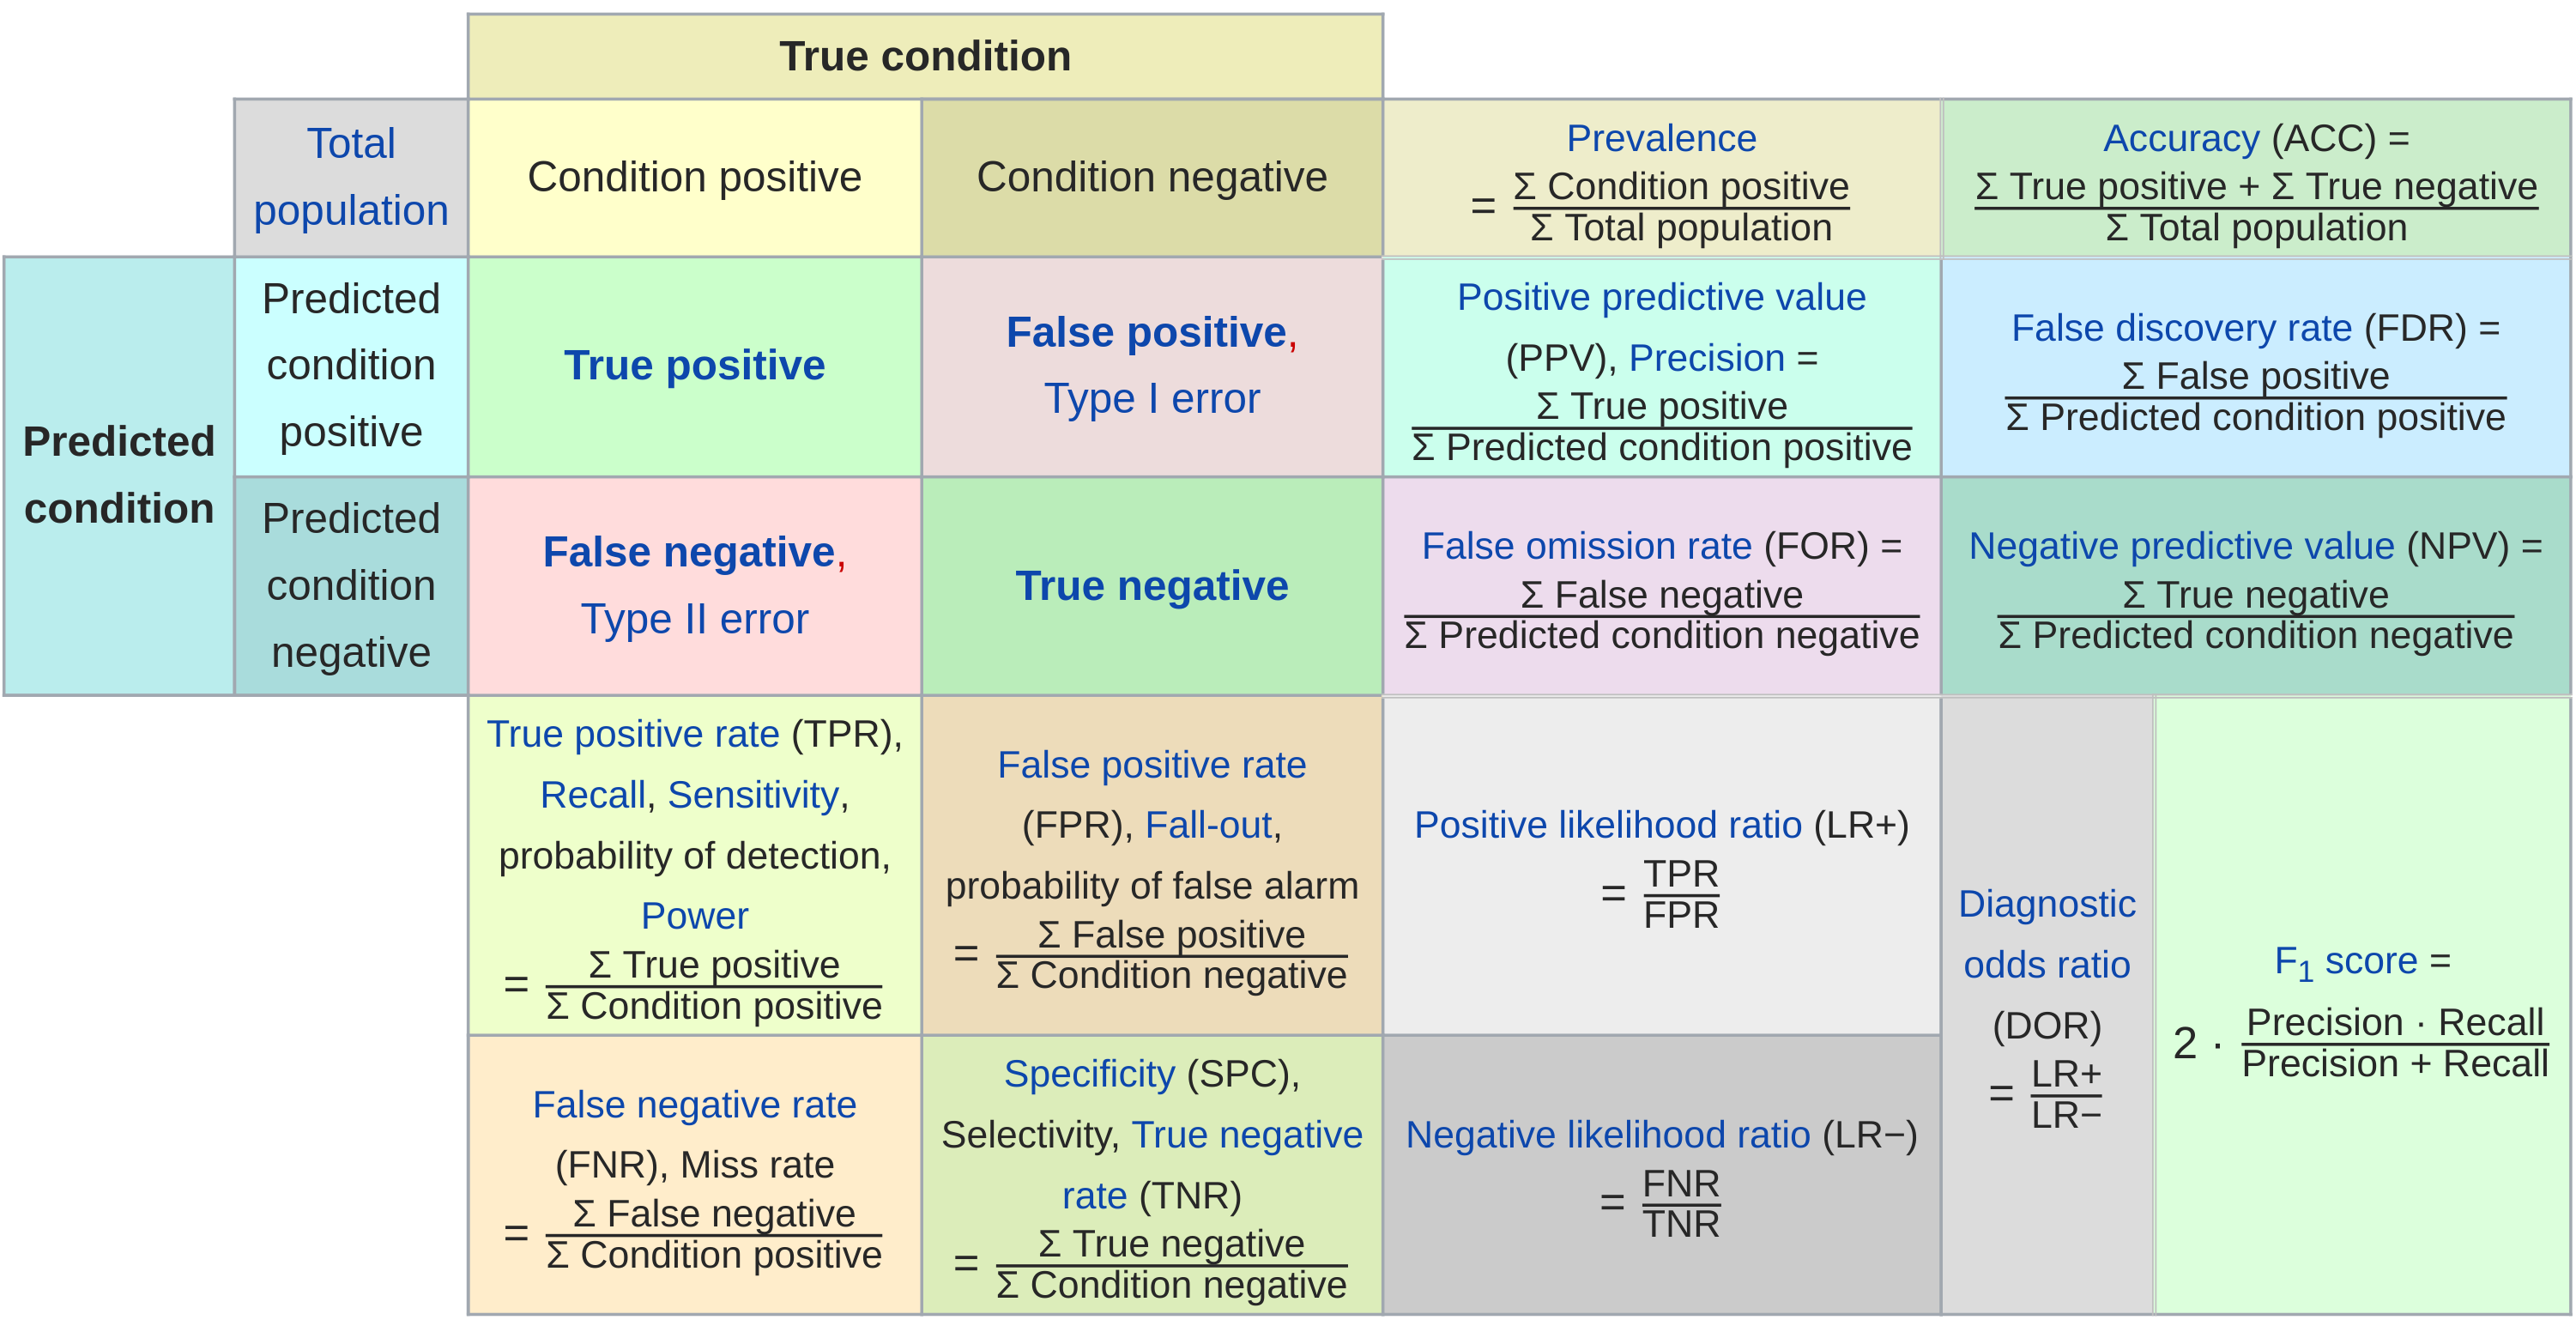
\includegraphics[width=0.98\linewidth]{images/confusion_matrix(wikipedia)} \end{center}

Source: \href{https://en.wikipedia.org/wiki/Evaluation_of_binary_classifiers}{Wikipedia}

It is difficult to achieve a high TPR and low FPR in conjunction, so one uses them for constructing the ROC Curve.
We characterize a classifier by its TPR and FPR values and plot them in a coordinate system.
The best classifier lies on the top-left corner.
The worst classifier lies at the diagonal.
Classifiers lying on the diagonal produce random labels (with different proportions).
If each positive \(x\) will be randomly classified with 25\% as ``positive'', we get a TPR of 0.25.
If we assign each negative \(x\) randomly to ``positive'' we get a FPR of 0.25.
In practice, we should never obtain a classifier below the diagonal, as inverting the predicted labels will result in a reflection at the diagonal.

A scoring classifier is a model which produces scores or probabilities, instead of discrete labels.
Nearly all modern classifiers can do that.
Thresholding flexibly converts measured probabilities to labels.
Predict \(1\) (positive class) if \(\hat{f}(x) > \tau\) else predict \(0\).
Normally, one could use \(\tau = 0.5\) to convert probabilities to labels, but for imbalanced or cost-sensitive situations another threshold could be more suitable.
After thresholding, any metric defined on labels can be used.

For \href{https://mlr3.mlr-org.com}{mlr3} prediction objects, the ROC curve can easily be created with \href{https://mlr3viz.mlr-org.com}{mlr3viz} which relies on the \texttt{precrec} to calculate and plot ROC curves:

\begin{Shaded}
\begin{Highlighting}[]
\CommentTok{# TPR vs FPR / Sensitivity vs (1 - Specificity)}
\NormalTok{ggplot2}\OperatorTok{::}\KeywordTok{autoplot}\NormalTok{(pred, }\DataTypeTok{type =} \StringTok{"roc"}\NormalTok{)}
\end{Highlighting}
\end{Shaded}

\begin{center}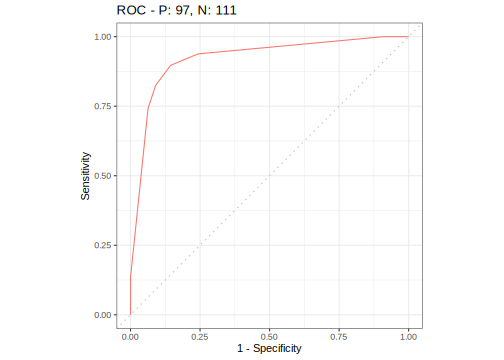
\includegraphics{mlr3book_files/figure-latex/02-basics-074-1} \end{center}

\begin{Shaded}
\begin{Highlighting}[]

\CommentTok{# Precision vs Recall}
\NormalTok{ggplot2}\OperatorTok{::}\KeywordTok{autoplot}\NormalTok{(pred, }\DataTypeTok{type =} \StringTok{"prc"}\NormalTok{)}
\end{Highlighting}
\end{Shaded}

\begin{center}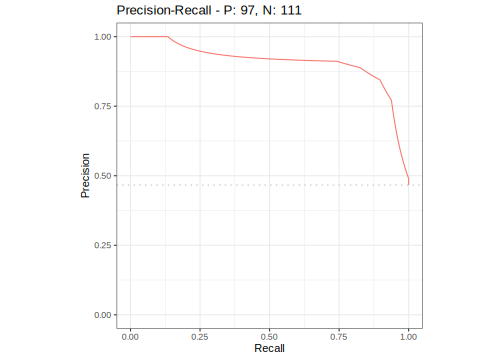
\includegraphics{mlr3book_files/figure-latex/02-basics-074-2} \end{center}

\hypertarget{threshold-tuning}{%
\subsection{Threshold Tuning}\label{threshold-tuning}}

\hypertarget{model-optim}{%
\chapter{Model Optimization}\label{model-optim}}

\protect\hyperlink{tuning}{\textbf{Model Tuning}}

Machine learning algorithms have default values set for their hyperparameters.
Irrespective, these hyperparameters need to be changed by the user to achieve optimal performance on the given dataset.
A manual selection of hyperparameter values is not recommended as this approach rarely leads to an optimal performance.
To substantiate the validity of the selected hyperparatmeters (= \protect\hyperlink{tuning}{tuning}), data-driven optimization is recommended.
In order to tune a machine learning algorithm, one has to specify (1) the \protect\hyperlink{tuning-optimization}{search space}, (2) the \protect\hyperlink{tuning-optimization}{optimization algorithm} (aka tuning method) and (3) an evaluation method, i.e., a resampling strategy and a performance measure.

In summary, the sub-chapter on \protect\hyperlink{tuning}{tuning} illustrates how to:

\begin{itemize}
\tightlist
\item
  undertake empirically sound \protect\hyperlink{tuning}{hyperparameter selection}
\item
  select the \protect\hyperlink{tuning-optimization}{optimizing algorithm}
\item
  \protect\hyperlink{tuning-triggering}{trigger} the tuning
\item
  \protect\hyperlink{autotuner}{automate} tuning
\end{itemize}

This \protect\hyperlink{tuning}{sub-chapter} requires the package \texttt{mlr3-tuning}, an extension package which supports hyperparameter tuning.

\protect\hyperlink{fs}{\textbf{Feature Selection}}

The second part of this chapter explains \protect\hyperlink{fs}{feature selection}.
The objective of \protect\hyperlink{fs}{feature selection} is to fit the sparse dependent of a model on a subset of available data features in the most suitable manner.
\protect\hyperlink{fs}{Feature selection} can enhance the interpretability of the model, speed up model fitting and improve the learner performance by reducing noise in the data.
Different approaches exist to identify the relevant features.
In the sub-chapter on \protect\hyperlink{fs}{feature selection}, three approaches are emphasized:

\begin{itemize}
\tightlist
\item
  Feature selection using \protect\hyperlink{fs-filter}{filter} algorithms
\item
  Feature selection via \protect\hyperlink{fs-var-imp-filter}{variable importance filters}
\item
  Feature selection by employing the so called \protect\hyperlink{fs-wrapper}{wrapper methods}
\end{itemize}

A fourth approach, feature selection via \protect\hyperlink{fs-ensemble}{ensemble filters}, is introduced subsequently.
The implementation of all four approaches in mlr3 is showcased using the extension-package \href{https://mlr3filters.mlr-org.com}{mlr3filters}.

\protect\hyperlink{nested-resampling}{\textbf{Nested Resampling}}

In order to get a good estimate of generalization performance and avoid data leakage, both an outer (performance) and an inner (tuning/feature selection) resampling process are necessary.
Following features are discussed in this chapter:

\begin{itemize}
\tightlist
\item
  Inner and outer resampling strategies in \protect\hyperlink{nested-resampling}{nested resampling}
\item
  The \protect\hyperlink{nested-resamp-exec}{execution} of nested resampling
\item
  The \protect\hyperlink{nested-resamp-eval}{evaluation} of executed resampling iterations
\end{itemize}

The sub-section \protect\hyperlink{nested-resampling}{nested resampling} will provide instructions on how to implement nested resampling, accounting for both inner and outer resampling in mlr3.

\hypertarget{tuning}{%
\section{Hyperparameter Tuning}\label{tuning}}

Hyperparameter tuning is supported via the extension package \href{https://mlr3tuning.mlr-org.com}{mlr3tuning}.
The heart of \href{https://mlr3tuning.mlr-org.com}{mlr3tuning} are the R6 classes:

\begin{itemize}
\tightlist
\item
  \texttt{TuningInstance}: This class describes the tuning problem and stores results.
\item
  \texttt{Tuner}: This class is the base class for implementations of tuning algorithms.
\end{itemize}

\hypertarget{tuning-optimization}{%
\subsection{\texorpdfstring{The \texttt{TuningInstance} Class}{The TuningInstance Class}}\label{tuning-optimization}}

The following sub-section examines the optimization of a simple classification tree on the \texttt{mlr\_tasks\_pima",\ text\ =\ "Pima\ Indian\ Diabetes} data set.

\begin{Shaded}
\begin{Highlighting}[]
\NormalTok{task =}\StringTok{ }\KeywordTok{tsk}\NormalTok{(}\StringTok{"pima"}\NormalTok{)}
\KeywordTok{print}\NormalTok{(task)}
\NormalTok{## <TaskClassif:pima> (768 x 9)}
\NormalTok{## * Target: diabetes}
\NormalTok{## * Properties: twoclass}
\NormalTok{## * Features (8):}
\NormalTok{##   - dbl (8): age, glucose, insulin, mass,}
\NormalTok{##     pedigree, pregnant, pressure, triceps}
\end{Highlighting}
\end{Shaded}

We use the classification tree from \texttt{rpart} and choose a subset of the hyperparameters we want to tune.
This is often referred to as the ``tuning space''.

\begin{Shaded}
\begin{Highlighting}[]
\NormalTok{learner =}\StringTok{ }\KeywordTok{lrn}\NormalTok{(}\StringTok{"classif.rpart"}\NormalTok{)}
\NormalTok{learner}\OperatorTok{$}\NormalTok{param_set}
\NormalTok{## ParamSet: }
\NormalTok{##              id    class lower upper levels default}
\NormalTok{## 1:     minsplit ParamInt     1   Inf             20}
\NormalTok{## 2:           cp ParamDbl     0     1           0.01}
\NormalTok{## 3:   maxcompete ParamInt     0   Inf              4}
\NormalTok{## 4: maxsurrogate ParamInt     0   Inf              5}
\NormalTok{## 5:     maxdepth ParamInt     1    30             30}
\NormalTok{## 6:         xval ParamInt     0   Inf             10}
\NormalTok{##    value}
\NormalTok{## 1:      }
\NormalTok{## 2:      }
\NormalTok{## 3:      }
\NormalTok{## 4:      }
\NormalTok{## 5:      }
\NormalTok{## 6:     0}
\end{Highlighting}
\end{Shaded}

Here, we opt to tune two parameters namely on the one hand the complexity \texttt{cp} and second of all the termination criterion \texttt{minsplit}.
As the tuning space has to be bound,one needs to set lower and upper bounds:

\begin{Shaded}
\begin{Highlighting}[]
\KeywordTok{library}\NormalTok{(paradox)}
\NormalTok{tune_ps =}\StringTok{ }\NormalTok{ParamSet}\OperatorTok{$}\KeywordTok{new}\NormalTok{(}\KeywordTok{list}\NormalTok{(ParamDbl}\OperatorTok{$}\KeywordTok{new}\NormalTok{(}\StringTok{"cp"}\NormalTok{, }\DataTypeTok{lower =} \FloatTok{0.001}\NormalTok{, }
  \DataTypeTok{upper =} \FloatTok{0.1}\NormalTok{), ParamInt}\OperatorTok{$}\KeywordTok{new}\NormalTok{(}\StringTok{"minsplit"}\NormalTok{, }\DataTypeTok{lower =} \DecValTok{1}\NormalTok{, }\DataTypeTok{upper =} \DecValTok{10}\NormalTok{)))}
\NormalTok{tune_ps}
\NormalTok{## ParamSet: }
\NormalTok{##          id    class lower upper levels     default}
\NormalTok{## 1:       cp ParamDbl 0.001   0.1        <NoDefault>}
\NormalTok{## 2: minsplit ParamInt 1.000  10.0        <NoDefault>}
\NormalTok{##    value}
\NormalTok{## 1:      }
\NormalTok{## 2:}
\end{Highlighting}
\end{Shaded}

Next, we are able to define how to evaluate the performance.
In order to determine the evaluation method, one has to choose a \texttt{Resampling",\ text\ =\ "resampling\ strategy} and a \texttt{Measure",\ text\ =\ "performance\ measure}.

\begin{Shaded}
\begin{Highlighting}[]
\NormalTok{hout =}\StringTok{ }\KeywordTok{rsmp}\NormalTok{(}\StringTok{"holdout"}\NormalTok{)}
\NormalTok{measure =}\StringTok{ }\KeywordTok{msr}\NormalTok{(}\StringTok{"classif.ce"}\NormalTok{)}
\end{Highlighting}
\end{Shaded}

Finally, one has to select the budget available, to solve this tuning instance.
This is done by selecting one of the available \texttt{Terminator",\ text\ =\ "Terminators}:

\begin{itemize}
\tightlist
\item
  Terminate after a given time (\texttt{TerminatorClockTime})
\item
  Terminate after a given amount of iterations (\texttt{TerminatorEvals})
\item
  Terminate after a specific performance is reached (\texttt{TerminatorPerfReached})
\item
  Terminate when tuning does not improve (\texttt{TerminatorStagnation})
\item
  A combination of the above in an \emph{ALL} or \emph{ANY} fashion, using \texttt{TerminatorCombo}
\end{itemize}

For this short introduction, we grant a budget of 20 evaluations and then put everything together into a \texttt{TuningInstance}:

\begin{Shaded}
\begin{Highlighting}[]
\KeywordTok{library}\NormalTok{(mlr3tuning)}

\NormalTok{evals20 =}\StringTok{ }\KeywordTok{term}\NormalTok{(}\StringTok{"evals"}\NormalTok{, }\DataTypeTok{n_evals =} \DecValTok{20}\NormalTok{)}

\NormalTok{instance =}\StringTok{ }\NormalTok{TuningInstance}\OperatorTok{$}\KeywordTok{new}\NormalTok{(}\DataTypeTok{task =}\NormalTok{ task, }\DataTypeTok{learner =}\NormalTok{ learner, }
  \DataTypeTok{resampling =}\NormalTok{ hout, }\DataTypeTok{measures =}\NormalTok{ measure, }\DataTypeTok{param_set =}\NormalTok{ tune_ps, }
  \DataTypeTok{terminator =}\NormalTok{ evals20)}
\KeywordTok{print}\NormalTok{(instance)}
\NormalTok{## <TuningInstance>}
\NormalTok{## * Task: <TaskClassif:pima>}
\NormalTok{## * Learner: <LearnerClassifRpart:classif.rpart>}
\NormalTok{## * Measures: classif.ce}
\NormalTok{## * Resampling: <ResamplingHoldout>}
\NormalTok{## * Terminator: <TerminatorEvals>}
\NormalTok{## * bm_args: list()}
\NormalTok{## ParamSet: }
\NormalTok{##          id    class lower upper levels     default}
\NormalTok{## 1:       cp ParamDbl 0.001   0.1        <NoDefault>}
\NormalTok{## 2: minsplit ParamInt 1.000  10.0        <NoDefault>}
\NormalTok{##    value}
\NormalTok{## 1:      }
\NormalTok{## 2:      }
\NormalTok{## Archive:}
\NormalTok{## Empty data.table (0 rows and 11 cols): nr,batch_nr,resample_result,task_id,learner_id,resampling_id...}
\end{Highlighting}
\end{Shaded}

To start the tuning, we still need to select how the optimization should take place.
In other words, we need to choose the \textbf{optimization algorithm} via the \texttt{Tuner} class.

\hypertarget{the-tuner-class}{%
\subsection{\texorpdfstring{The \texttt{Tuner} Class}{The Tuner Class}}\label{the-tuner-class}}

The following algorithms are currently implemented in \href{https://mlr3tuning.mlr-org.com}{mlr3tuning}:

\begin{itemize}
\tightlist
\item
  Grid Search (\texttt{TunerGridSearch})
\item
  Random Search (\texttt{TunerRandomSearch}) (Bergstra and Bengio \protect\hyperlink{ref-bergstra2012}{2012})
\item
  Generalized Simulated Annealing (\texttt{TunerGenSA})
\end{itemize}

In this example, we will use a simple grid search with a grid resolution of 10:

\begin{Shaded}
\begin{Highlighting}[]
\NormalTok{tuner =}\StringTok{ }\KeywordTok{tnr}\NormalTok{(}\StringTok{"grid_search"}\NormalTok{, }\DataTypeTok{resolution =} \DecValTok{5}\NormalTok{)}
\end{Highlighting}
\end{Shaded}

Since we have only numeric parameters, \texttt{TunerGridSearch} will create a grid of equally-sized steps between the respective upper and lower bounds.
As we have two hyperparameters with a resolution of 5, the two-dimensional grid consists of \(5^2 = 25\) configurations.
Each configuration serves as hyperparameter setting for the classification tree and triggers a 3-fold cross validation on the task.
All configurations will be examined by the tuner (in a random order), until either all configurations are evaluated or the \texttt{Terminator} signals that the budget is exhausted.

\hypertarget{tuning-triggering}{%
\subsection{Triggering the Tuning}\label{tuning-triggering}}

To start the tuning, we simply pass the \texttt{TuningInstance} to the \texttt{\$tune()} method of the initialized \texttt{Tuner}.
The tuner proceeds as follow:

\begin{enumerate}
\def\labelenumi{\arabic{enumi}.}
\tightlist
\item
  The \texttt{Tuner} proposes at least one hyperparameter configuration (the \texttt{Tuner} and may propose multiple points to improve parallelization, which can be controlled via the setting \texttt{batch\_size}).
\item
  For each configuration, a \texttt{Learner} is fitted on \texttt{Task} using the provided \texttt{Resampling}.
  The results are combined with other results from previous iterations to a single \texttt{BenchmarkResult}.
\item
  The \texttt{Terminator} is queried if the budget is exhausted.
  If the budget is not exhausted, restart with 1) until it is.
\item
  Determine the configuration with the best observed performance.
\item
  Return a named list with the hyperparameter settings (\texttt{"values"}) and the corresponding measured performance (\texttt{"performance"}).
\end{enumerate}

\begin{Shaded}
\begin{Highlighting}[]
\NormalTok{result =}\StringTok{ }\NormalTok{tuner}\OperatorTok{$}\KeywordTok{tune}\NormalTok{(instance)}
\KeywordTok{print}\NormalTok{(result)}
\NormalTok{## NULL}
\end{Highlighting}
\end{Shaded}

One can investigate all resamplings which where undertaken, using the \texttt{\$archive()} method of the \texttt{TuningInstance}.
Here, we just extract the performance values and the hyperparameters:

\begin{Shaded}
\begin{Highlighting}[]
\NormalTok{instance}\OperatorTok{$}\KeywordTok{archive}\NormalTok{(}\DataTypeTok{unnest =} \StringTok{"params"}\NormalTok{)[, }\KeywordTok{c}\NormalTok{(}\StringTok{"cp"}\NormalTok{, }\StringTok{"minsplit"}\NormalTok{, }
  \StringTok{"classif.ce"}\NormalTok{)]}
\NormalTok{##          cp minsplit classif.ce}
\NormalTok{##  1: 0.00100        3     0.3008}
\NormalTok{##  2: 0.10000        8     0.3008}
\NormalTok{##  3: 0.10000       10     0.3008}
\NormalTok{##  4: 0.07525        1     0.3008}
\NormalTok{##  5: 0.00100        8     0.2773}
\NormalTok{##  6: 0.02575        1     0.2305}
\NormalTok{##  7: 0.10000        3     0.3008}
\NormalTok{##  8: 0.05050       10     0.3008}
\NormalTok{##  9: 0.10000        5     0.3008}
\NormalTok{## 10: 0.07525       10     0.3008}
\NormalTok{## 11: 0.07525        8     0.3008}
\NormalTok{## 12: 0.07525        3     0.3008}
\NormalTok{## 13: 0.02575        8     0.2305}
\NormalTok{## 14: 0.05050        5     0.3008}
\NormalTok{## 15: 0.02575        3     0.2305}
\NormalTok{## 16: 0.07525        5     0.3008}
\NormalTok{## 17: 0.00100        1     0.3164}
\NormalTok{## 18: 0.00100        5     0.2969}
\NormalTok{## 19: 0.05050        1     0.3008}
\NormalTok{## 20: 0.05050        3     0.3008}
\end{Highlighting}
\end{Shaded}

In sum, the grid search evaluated 20/25 different configurations of the grid in a random order before the \texttt{Terminator} stopped the tuning.

Now the optimized hyperparameters can take the previously created \texttt{Learner}, set the returned hyperparameters and \protect\hyperlink{train-predict}{train} it on the full dataset.

\begin{Shaded}
\begin{Highlighting}[]
\NormalTok{learner}\OperatorTok{$}\NormalTok{param_set}\OperatorTok{$}\NormalTok{values =}\StringTok{ }\NormalTok{instance}\OperatorTok{$}\NormalTok{result}\OperatorTok{$}\NormalTok{params}
\NormalTok{learner}\OperatorTok{$}\KeywordTok{train}\NormalTok{(task)}
\end{Highlighting}
\end{Shaded}

The trained model could now be used to make a prediction on external data.
Note that predicting on observations present in the \texttt{task}, is statistically bias and should be avoided.
The model has already seen these observations during the tuning process.
Hence, the resulting performance measure would be over-optimistic.
Instead, to get unbiased performance estimates for the current task, \protect\hyperlink{nested-resamling}{nested resampling} is required.

\hypertarget{autotuner}{%
\subsection{Automating the Tuning}\label{autotuner}}

The \texttt{AutoTuner} wraps a learner and augments it with an automatic tuning for a given set of hyperparameters.
Because the \texttt{AutoTuner} itself inherits from the \texttt{Learner} base class, it can be used like any other learner.
Analogously to the previous subsection, a new classification tree learner is created.
This classification tree learner automatically tunes the parameters \texttt{cp} and \texttt{minsplit} using an inner resampling (holdout).
We create a terminator which allows 10 evaluations, and use a simple random search as tuning algorithm:

\begin{Shaded}
\begin{Highlighting}[]
\KeywordTok{library}\NormalTok{(paradox)}
\KeywordTok{library}\NormalTok{(mlr3tuning)}

\NormalTok{learner =}\StringTok{ }\KeywordTok{lrn}\NormalTok{(}\StringTok{"classif.rpart"}\NormalTok{)}
\NormalTok{resampling =}\StringTok{ }\KeywordTok{rsmp}\NormalTok{(}\StringTok{"holdout"}\NormalTok{)}
\NormalTok{measures =}\StringTok{ }\KeywordTok{msr}\NormalTok{(}\StringTok{"classif.ce"}\NormalTok{)}
\NormalTok{tune_ps =}\StringTok{ }\NormalTok{ParamSet}\OperatorTok{$}\KeywordTok{new}\NormalTok{(}\KeywordTok{list}\NormalTok{(ParamDbl}\OperatorTok{$}\KeywordTok{new}\NormalTok{(}\StringTok{"cp"}\NormalTok{, }\DataTypeTok{lower =} \FloatTok{0.001}\NormalTok{, }
  \DataTypeTok{upper =} \FloatTok{0.1}\NormalTok{), ParamInt}\OperatorTok{$}\KeywordTok{new}\NormalTok{(}\StringTok{"minsplit"}\NormalTok{, }\DataTypeTok{lower =} \DecValTok{1}\NormalTok{, }\DataTypeTok{upper =} \DecValTok{10}\NormalTok{)))}
\NormalTok{terminator =}\StringTok{ }\KeywordTok{term}\NormalTok{(}\StringTok{"evals"}\NormalTok{, }\DataTypeTok{n_evals =} \DecValTok{10}\NormalTok{)}
\NormalTok{tuner =}\StringTok{ }\KeywordTok{tnr}\NormalTok{(}\StringTok{"random_search"}\NormalTok{)}

\NormalTok{at =}\StringTok{ }\NormalTok{AutoTuner}\OperatorTok{$}\KeywordTok{new}\NormalTok{(}\DataTypeTok{learner =}\NormalTok{ learner, }\DataTypeTok{resampling =}\NormalTok{ resampling, }
  \DataTypeTok{measures =}\NormalTok{ measures, }\DataTypeTok{tune_ps =}\NormalTok{ tune_ps, }\DataTypeTok{terminator =}\NormalTok{ terminator, }
  \DataTypeTok{tuner =}\NormalTok{ tuner)}
\NormalTok{at}
\NormalTok{## <AutoTuner:classif.rpart.tuned>}
\NormalTok{## * Model: -}
\NormalTok{## * Parameters: xval=0}
\NormalTok{## * Packages: rpart}
\NormalTok{## * Predict Type: response}
\NormalTok{## * Feature types: logical, integer, numeric,}
\NormalTok{##   factor, ordered}
\NormalTok{## * Properties: importance, missings, multiclass,}
\NormalTok{##   selected_features, twoclass, weights}
\end{Highlighting}
\end{Shaded}

We can now use the learner like any other learner, calling the \texttt{\$train()} and \texttt{\$predict()} method.
This time however, we pass it to \texttt{benchmark()} to compare the tuner to a classification tree without tuning.
This way, the \texttt{AutoTuner} will do its resampling for tuning on the training set of the respective split of the outer resampling.
The learner then predicts using the test set of the outer resampling.
This yields unbiased performance measures, as the observations in the test set have not been used during tuning or fitting of the respective learner.
This is called \protect\hyperlink{nested-resampling}{nested resampling}.

To compare the tuned learner with the learner using its default, we can use \texttt{benchmark()}:

\begin{Shaded}
\begin{Highlighting}[]
\NormalTok{grid =}\StringTok{ }\KeywordTok{benchmark_grid}\NormalTok{(}\DataTypeTok{task =} \KeywordTok{tsk}\NormalTok{(}\StringTok{"pima"}\NormalTok{), }\DataTypeTok{learner =} \KeywordTok{list}\NormalTok{(at, }
  \KeywordTok{lrn}\NormalTok{(}\StringTok{"classif.rpart"}\NormalTok{)), }\DataTypeTok{resampling =} \KeywordTok{rsmp}\NormalTok{(}\StringTok{"cv"}\NormalTok{, }\DataTypeTok{folds =} \DecValTok{3}\NormalTok{))}
\NormalTok{bmr =}\StringTok{ }\KeywordTok{benchmark}\NormalTok{(grid)}
\NormalTok{bmr}\OperatorTok{$}\KeywordTok{aggregate}\NormalTok{(measures)}
\NormalTok{##    nr  resample_result task_id          learner_id}
\NormalTok{## 1:  1 <ResampleResult>    pima classif.rpart.tuned}
\NormalTok{## 2:  2 <ResampleResult>    pima       classif.rpart}
\NormalTok{##    resampling_id iters classif.ce}
\NormalTok{## 1:            cv     3     0.2643}
\NormalTok{## 2:            cv     3     0.2617}
\end{Highlighting}
\end{Shaded}

Note that we do not expect any differences compared to the non-tuned approach for multiple reasons:

\begin{itemize}
\tightlist
\item
  the task is too easy
\item
  the task is rather small, and thus prone to overfitting
\item
  the tuning budget (10 evaluations) is small
\item
  \texttt{rpart} does not benefit that much from tuning
\end{itemize}

\hypertarget{fs}{%
\section{Feature Selection / Filtering}\label{fs}}

Often, data sets include a large number of features.
The technique of extracting a subset of relevant features is called ``feature selection''.
The objective of feature selection is to fit the sparse dependent of a model on a subset of available data features in the most suitable manner.
Feature selection can enhance the interpretability of the model, speed up the learning process and improve the learner performance.
Different approaches exist to identify the relevant features.
In the literature two distinct approaches are emphasized:
One is called \protect\hyperlink{fs-filtering}{Filtering} and the other approach is often referred to as feature subset selection or \protect\hyperlink{fs-wrapper}{wrapper methods}.

What are the differences (Chandrashekar and Sahin \protect\hyperlink{ref-chandrashekar2014}{2014})?

\begin{itemize}
\tightlist
\item
  \textbf{Filtering}: An external algorithm computes a rank of the variables (e.g.~based on the correlation to the response).
  Then, features are subsetted by a certain criteria, e.g.~an absolute number or a percentage of the number of variables.
  The selected features will then be used to fit a model (with optional hyperparameters selected by tuning).
  This calculation is usually cheaper than ``feature subset selection'' in terms of computation time.
\item
  \textbf{Wrapper Methods}: Here, no ranking of features is done.
  Features are selected by a (random) subset of the data.
  Then, we fit a model and subseqeuently assess the performance.
  This is done for a lot of feature combinations in a cross-validation (CV) setting and the best combination is reported.
  This method is very computational intense as a lot of models are fitted.
  Also, strictly speaking all these models would need to be tuned before the performance is estimated.
  This would require an additional nested level in a CV setting.
  After undertaken all of these steps, the selected subset of features is again fitted (with optional hyperparameters selected by tuning).
\end{itemize}

There is also a third approach which can be attributed to the ``filter'' family:
The embedded feature-selection methods of some \texttt{Learner}.
Read more about how to use these in section \protect\hyperlink{fs-embedded}{embedded feature-selection methods}.

\href{\%7B\#fs-ensemble\%7D}{Ensemble filters} built upon the idea of stacking single filter methods.
These are not yet implemented.

All functionality that is related to feature selection is implemented via the extension package \texttt{mlr-org/mlr3filters}.

\hypertarget{fs-filter}{%
\subsection{Filters}\label{fs-filter}}

Filter methods assign an importance value to each feature.
Based on these values the features can be ranked.
Thereafter, we are able to select a feature subset.
There is a list of all implemented filter methods in the \protect\hyperlink{list-filters}{Appendix}.

\hypertarget{fs-calc}{%
\subsection{Calculating filter values}\label{fs-calc}}

Currently, only classification and regression tasks are supported.

The first step it to create a new R object using the class of the desired filter method.
Each object of class \texttt{Filter} has a \texttt{.\$calculate()} method which calculates the filter values and ranks them in a descending order.

\begin{Shaded}
\begin{Highlighting}[]
\KeywordTok{library}\NormalTok{(mlr3filters)}
\NormalTok{filter =}\StringTok{ }\NormalTok{FilterJMIM}\OperatorTok{$}\KeywordTok{new}\NormalTok{()}

\NormalTok{task =}\StringTok{ }\KeywordTok{tsk}\NormalTok{(}\StringTok{"iris"}\NormalTok{)}
\NormalTok{filter}\OperatorTok{$}\KeywordTok{calculate}\NormalTok{(task)}

\KeywordTok{as.data.table}\NormalTok{(filter)}
\NormalTok{##         feature  score}
\NormalTok{## 1: Sepal.Length 1.0401}
\NormalTok{## 2:  Petal.Width 0.9894}
\NormalTok{## 3: Petal.Length 0.9881}
\NormalTok{## 4:  Sepal.Width 0.8314}
\end{Highlighting}
\end{Shaded}

Some filters support changing specific hyperparameters.
This is done similar to setting hyperparameters of a \texttt{Learner} using \texttt{.\$param\_set\$values}:

\begin{Shaded}
\begin{Highlighting}[]
\NormalTok{filter_cor =}\StringTok{ }\NormalTok{FilterCorrelation}\OperatorTok{$}\KeywordTok{new}\NormalTok{()}
\NormalTok{filter_cor}\OperatorTok{$}\NormalTok{param_set}
\NormalTok{## ParamSet: }
\NormalTok{##        id    class lower upper}
\NormalTok{## 1:    use ParamFct    NA    NA}
\NormalTok{## 2: method ParamFct    NA    NA}
\NormalTok{##                                                                  levels}
\NormalTok{## 1: everything,all.obs,complete.obs,na.or.complete,pairwise.complete.obs}
\NormalTok{## 2:                                             pearson,kendall,spearman}
\NormalTok{##       default value}
\NormalTok{## 1: everything      }
\NormalTok{## 2:    pearson}

\CommentTok{# change parameter 'method'}
\NormalTok{filter_cor}\OperatorTok{$}\NormalTok{param_set}\OperatorTok{$}\NormalTok{values =}\StringTok{ }\KeywordTok{list}\NormalTok{(}\DataTypeTok{method =} \StringTok{"spearman"}\NormalTok{)}
\NormalTok{filter_cor}\OperatorTok{$}\NormalTok{param_set}
\NormalTok{## ParamSet: }
\NormalTok{##        id    class lower upper}
\NormalTok{## 1:    use ParamFct    NA    NA}
\NormalTok{## 2: method ParamFct    NA    NA}
\NormalTok{##                                                                  levels}
\NormalTok{## 1: everything,all.obs,complete.obs,na.or.complete,pairwise.complete.obs}
\NormalTok{## 2:                                             pearson,kendall,spearman}
\NormalTok{##       default    value}
\NormalTok{## 1: everything         }
\NormalTok{## 2:    pearson spearman}
\end{Highlighting}
\end{Shaded}

Rather than taking the ``long'' R6 way to create a filter, there is also a built-in shorthand notation for filter creation:

\begin{Shaded}
\begin{Highlighting}[]
\NormalTok{filter =}\StringTok{ }\KeywordTok{flt}\NormalTok{(}\StringTok{"cmim"}\NormalTok{)}
\NormalTok{filter}
\NormalTok{## <FilterCMIM:cmim>}
\NormalTok{## Task Types: classif, regr}
\NormalTok{## Task Properties: -}
\NormalTok{## Packages: praznik}
\NormalTok{## Feature types: integer, numeric, factor, ordered}
\end{Highlighting}
\end{Shaded}

\hypertarget{fs-var-imp-filters}{%
\subsection{Variable Importance Filters}\label{fs-var-imp-filters}}

All \texttt{Learner} with the property ``importance'' come with integrated feature selection methods.

You can find a list of all learners with this property in the \protect\hyperlink{fs-filter-embedded-list}{Appendix}.

For some learners the desired filter method needs to be set during learner creation.
For example, learner \texttt{classif.ranger} (in the package \href{https://mlr3learners.mlr-org.com}{mlr3learners}) comes with multiple integrated methods.
See the help page of \texttt{ranger::ranger}.
To use method ``impurity'', you need to set the filter method during construction.

\begin{Shaded}
\begin{Highlighting}[]
\KeywordTok{library}\NormalTok{(mlr3learners)}
\NormalTok{lrn =}\StringTok{ }\KeywordTok{lrn}\NormalTok{(}\StringTok{"classif.ranger"}\NormalTok{, }\DataTypeTok{importance =} \StringTok{"impurity"}\NormalTok{)}
\end{Highlighting}
\end{Shaded}

Now you can use the \texttt{mlr3filters::FilterImportance} class for algorithm-embedded methods to filter a \texttt{Task}.

\begin{Shaded}
\begin{Highlighting}[]
\KeywordTok{library}\NormalTok{(mlr3learners)}

\NormalTok{task =}\StringTok{ }\KeywordTok{tsk}\NormalTok{(}\StringTok{"iris"}\NormalTok{)}
\NormalTok{filter =}\StringTok{ }\KeywordTok{flt}\NormalTok{(}\StringTok{"importance"}\NormalTok{, }\DataTypeTok{learner =}\NormalTok{ lrn)}
\NormalTok{filter}\OperatorTok{$}\KeywordTok{calculate}\NormalTok{(task)}
\KeywordTok{head}\NormalTok{(}\KeywordTok{as.data.table}\NormalTok{(filter), }\DecValTok{3}\NormalTok{)}
\NormalTok{##         feature score}
\NormalTok{## 1:  Petal.Width 43.60}
\NormalTok{## 2: Petal.Length 43.51}
\NormalTok{## 3: Sepal.Length 10.01}
\end{Highlighting}
\end{Shaded}

\hypertarget{fs-ensemble}{%
\subsection{Ensemble Methods}\label{fs-ensemble}}

\begin{warning}
Work in progress :)
\end{warning}

\hypertarget{fs-wrapper}{%
\subsection{Wrapper Methods}\label{fs-wrapper}}

\begin{warning}
Work in progress :) - via package \emph{mlr3fswrap}
\end{warning}

\hypertarget{nested-resampling}{%
\section{Nested Resampling}\label{nested-resampling}}

In order to obtain unbiased performance estimates for learners, all parts of the model building (preprocessing and model selection steps) should be included in the resampling, i.e., repeated for every pair of training/test data.
For steps that themselves require resampling like hyperparameter tuning or feature-selection (via the wrapper approach) this results in two nested resampling loops.

\begin{center}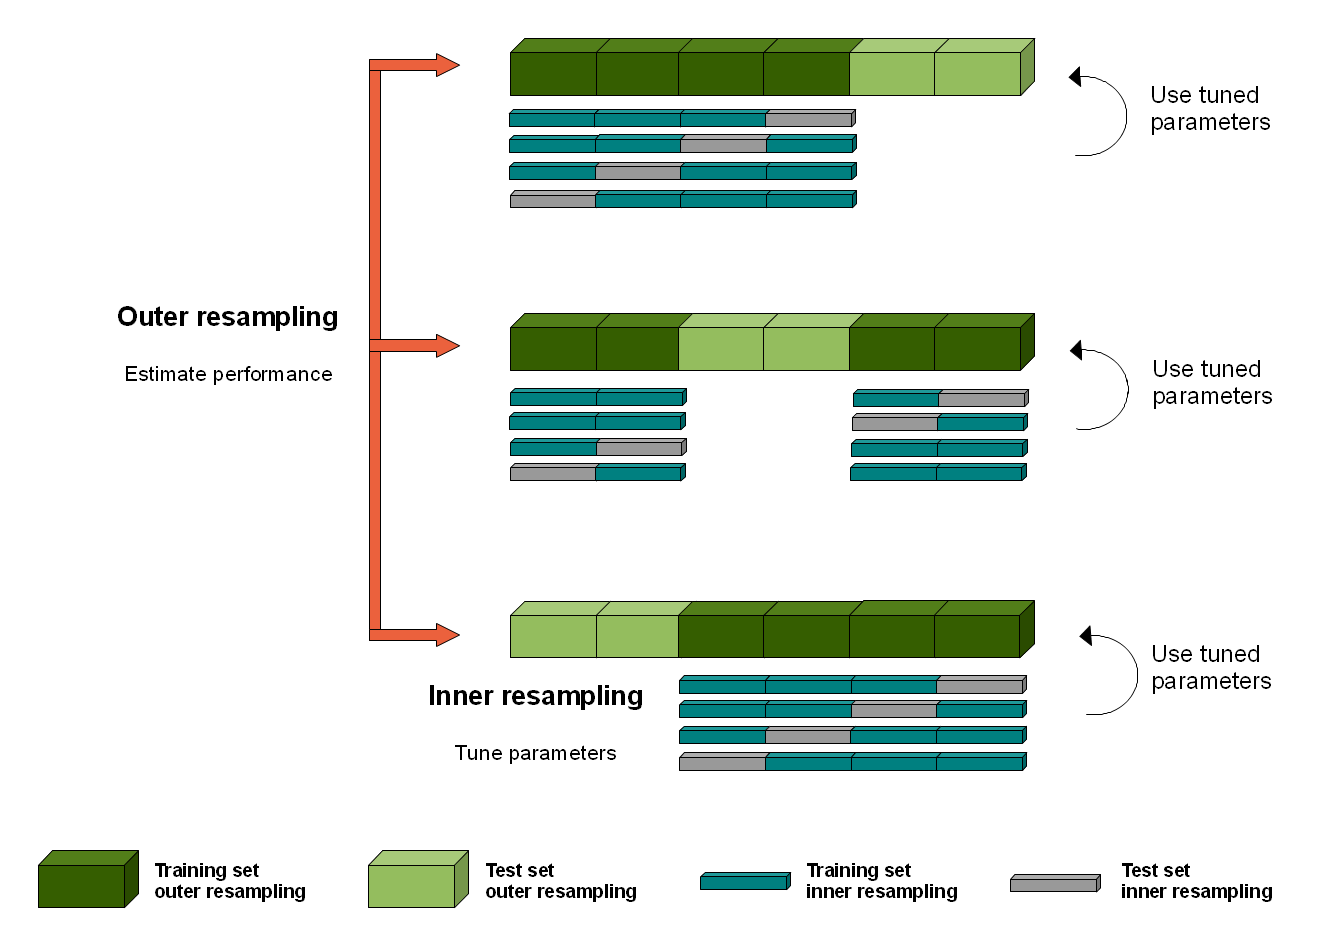
\includegraphics[width=0.98\linewidth]{images/nested_resampling} \end{center}

The graphic above illustrates nested resampling for parameter tuning with 3-fold cross-validation in the outer and 4-fold cross-validation in the inner loop.

In the outer resampling loop, we have three pairs of training/test sets.
On each of these outer training sets parameter tuning is done, thereby executing the inner resampling loop.
This way, we get one set of selected hyperparameters for each outer training set.
Then the learner is fitted on each outer training set using the corresponding selected hyperparameters.
Following, we can evaulate the performance of the learner on the outer test sets.

In \texttt{mlr-org/mlr3}, you can get nested resampling for free without programming any looping by using the \texttt{mlr3tuning::AutoTuner} class.
This works as follows:

\begin{enumerate}
\def\labelenumi{\arabic{enumi}.}
\tightlist
\item
  Generate a wrapped Learner via class \texttt{mlr3tuning::AutoTuner} or \texttt{mlr3filters::AutoSelect} (not yet implemented).
\item
  Specify all required settings - see section \protect\hyperlink{autotuner}{``Automating the Tuning''} for help.
\item
  Call function \texttt{resample()} or \texttt{benchmark()} with the created \texttt{Learner}.
\end{enumerate}

You can freely combine different inner and outer resampling strategies.

A common setup is prediction and performance evaluation on a fixed outer test set. This can be achieved by passing the \texttt{Resampling} strategy (\texttt{rsmp("holdout}) as the outer resampling instance to either \texttt{resample()} or \texttt{benchmark()}.

The inner resampling strategy could be a cross-validation one (\texttt{rsmp("cv}) as the sizes of the outer training sets might differ.
Per default, the inner resample description is instantiated once for every outer training set.

Note that nested resampling is computationally expensive.
For this reason we use relatively small search spaces and a low number of resampling iterations in the examples shown below.
In practice, you normally have to increase both.
As this is computationally intensive you might want to have a look at the section on \protect\hyperlink{parallelization}{Parallelization}.

\hypertarget{nested-resamp-exec}{%
\subsection{Execution}\label{nested-resamp-exec}}

To optimize hyperparameters or conduct feature selection in a nested resampling you need to create learners using either:

\begin{itemize}
\tightlist
\item
  the \texttt{AutoTuner} class, or
\item
  the \texttt{mlr3filters::AutoSelect} class (not yet implemented)
\end{itemize}

We use the example from section \protect\hyperlink{autotuner}{``Automating the Tuning''} and pipe the resulting learner into a \texttt{resample()} call.

\begin{Shaded}
\begin{Highlighting}[]
\KeywordTok{library}\NormalTok{(mlr3tuning)}
\NormalTok{task =}\StringTok{ }\KeywordTok{tsk}\NormalTok{(}\StringTok{"iris"}\NormalTok{)}
\NormalTok{learner =}\StringTok{ }\KeywordTok{lrn}\NormalTok{(}\StringTok{"classif.rpart"}\NormalTok{)}
\NormalTok{resampling =}\StringTok{ }\KeywordTok{rsmp}\NormalTok{(}\StringTok{"holdout"}\NormalTok{)}
\NormalTok{measures =}\StringTok{ }\KeywordTok{msr}\NormalTok{(}\StringTok{"classif.ce"}\NormalTok{)}
\NormalTok{param_set =}\StringTok{ }\NormalTok{paradox}\OperatorTok{::}\NormalTok{ParamSet}\OperatorTok{$}\KeywordTok{new}\NormalTok{(}\DataTypeTok{params =} \KeywordTok{list}\NormalTok{(paradox}\OperatorTok{::}\NormalTok{ParamDbl}\OperatorTok{$}\KeywordTok{new}\NormalTok{(}\StringTok{"cp"}\NormalTok{, }
  \DataTypeTok{lower =} \FloatTok{0.001}\NormalTok{, }\DataTypeTok{upper =} \FloatTok{0.1}\NormalTok{)))}
\NormalTok{terminator =}\StringTok{ }\KeywordTok{term}\NormalTok{(}\StringTok{"evals"}\NormalTok{, }\DataTypeTok{n_evals =} \DecValTok{5}\NormalTok{)}
\NormalTok{tuner =}\StringTok{ }\KeywordTok{tnr}\NormalTok{(}\StringTok{"grid_search"}\NormalTok{, }\DataTypeTok{resolution =} \DecValTok{10}\NormalTok{)}

\NormalTok{at =}\StringTok{ }\NormalTok{AutoTuner}\OperatorTok{$}\KeywordTok{new}\NormalTok{(learner, resampling, }\DataTypeTok{measures =}\NormalTok{ measures, }
\NormalTok{  param_set, terminator, }\DataTypeTok{tuner =}\NormalTok{ tuner)}
\end{Highlighting}
\end{Shaded}

Now construct the \texttt{resample()} call:

\begin{Shaded}
\begin{Highlighting}[]
\NormalTok{resampling_outer =}\StringTok{ }\KeywordTok{rsmp}\NormalTok{(}\StringTok{"cv"}\NormalTok{, }\DataTypeTok{folds =} \DecValTok{3}\NormalTok{)}
\NormalTok{rr =}\StringTok{ }\KeywordTok{resample}\NormalTok{(}\DataTypeTok{task =}\NormalTok{ task, }\DataTypeTok{learner =}\NormalTok{ at, }\DataTypeTok{resampling =}\NormalTok{ resampling_outer)}
\end{Highlighting}
\end{Shaded}

\hypertarget{nested-resamp-eval}{%
\subsection{Evaluation}\label{nested-resamp-eval}}

With the created \texttt{ResampleResult} we can now inspect the executed resampling iterations more closely.
See also section \protect\hyperlink{resampling}{Resampling} for more detailed information about \texttt{ResampleResult} objects.

For example, we can query the aggregated performance result:

\begin{Shaded}
\begin{Highlighting}[]
\NormalTok{rr}\OperatorTok{$}\KeywordTok{aggregate}\NormalTok{()}
\NormalTok{## classif.ce }
\NormalTok{##    0.07333}
\end{Highlighting}
\end{Shaded}

Check for any errors in the folds during execution (if there is not output, warnings or errors recorded, this is an empty \texttt{data.table()}:

\begin{Shaded}
\begin{Highlighting}[]
\NormalTok{rr}\OperatorTok{$}\NormalTok{errors}
\NormalTok{## Empty data.table (0 rows and 2 cols): iteration,msg}
\end{Highlighting}
\end{Shaded}

Or take a look at the confusion matrix of the joined predictions:

\begin{Shaded}
\begin{Highlighting}[]
\NormalTok{rr}\OperatorTok{$}\KeywordTok{prediction}\NormalTok{()}\OperatorTok{$}\NormalTok{confusion}
\NormalTok{##             truth}
\NormalTok{## response     setosa versicolor virginica}
\NormalTok{##   setosa         50          0         0}
\NormalTok{##   versicolor      0         44         5}
\NormalTok{##   virginica       0          6        45}
\end{Highlighting}
\end{Shaded}

\hypertarget{pipelines}{%
\chapter{Pipelines}\label{pipelines}}

\href{https://mlr3pipelines.mlr-org.com}{mlr3pipelines} is a dataflow programming toolkit.
This chapter focuses on the applicant's side of the package.
A more in-depth and technically oriented vignette can be found in the \href{https://mlr3pipelines.mlr-org.com/articles/introduction.html}{mlr3pipeline vignette}.

Machine learning workflows can be written as directed ``Graphs''/``Pipelines'' that represent data flows between preprocessing, model fitting, and ensemble learning units in an expressive and intuitive language.
We will most often use the term ``Graph'' in this manual but it can interchangeably be used with ``pipeline'' or ``workflow''.

An example for such a graph can be found below:

\begin{center}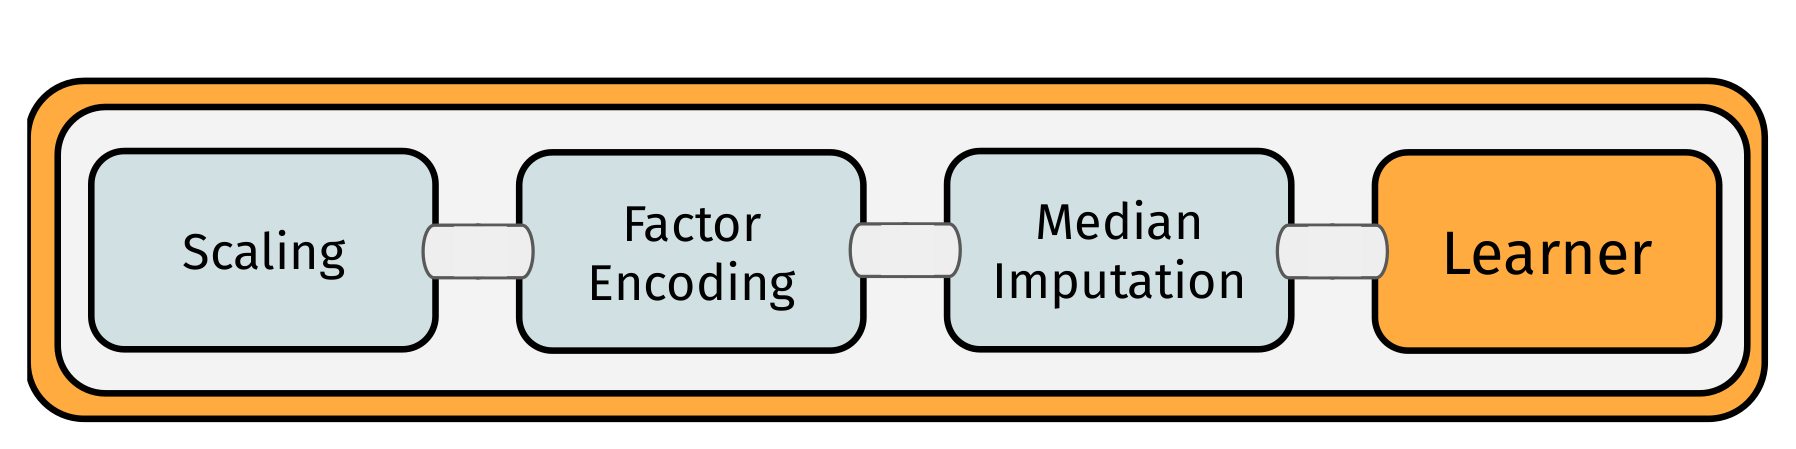
\includegraphics[width=0.98\linewidth]{images/simple_pipeline} \end{center}

Single computational steps can be represented as so-called PipeOps, which can then be connected with directed edges in a Graph.
The scope of \href{https://mlr3pipelines.mlr-org.com}{mlr3pipelines} is still growing.
Currently supported features are:

\begin{itemize}
\tightlist
\item
  Data manipulation and preprocessing operations, e.g.~PCA, feature filtering, imputation
\item
  Task subsampling for speed and outcome class imbalance handling
\item
  \href{https://mlr3.mlr-org.com}{mlr3} Learner operations for prediction and stacking
\item
  Ensemble methods and aggregation of predictions
\end{itemize}

Additionally, we implement several meta operators that can be used to construct powerful pipelines:

\begin{itemize}
\tightlist
\item
  Simultaneous path branching (data going both ways)
\item
  Alternative path branching (data going one specific way, controlled by hyperparameters)
\end{itemize}

An extensive introduction to creating custom \textbf{PipeOps} (PO's) can be found in the \protect\hyperlink{extending-mlr3pipelines}{technical introduction}.

Using methods from \href{https://mlr3tuning.mlr-org.com}{mlr3tuning}, it is even possible to simultaneously optimize parameters of multiple processing units.

A predecessor to this package is the \href{https://github.com/mlr-org/mlrCPO}{mlrCPO} package, which works with mlr 2.x.
Other packages that provide, to varying degree, some preprocessing functionality or machine learning domain specific language, are:

\begin{itemize}
\tightlist
\item
  the \texttt{caret} package and the related \texttt{recipes} project
\item
  the \texttt{dplyr} package
\end{itemize}

An example for a Pipeline that can be constructed using \href{https://mlr3pipelines.mlr-org.com}{mlr3pipelines} is depicted below:

\begin{center}\includegraphics{mlr3book_files/figure-latex/04-pipelines-002-1} \end{center}

\hypertarget{the-building-blocks-pipeops}{%
\section{The Building Blocks: PipeOps}\label{the-building-blocks-pipeops}}

The building blocks of \href{https://mlr3pipelines.mlr-org.com}{mlr3pipelines} are \textbf{PipeOp}-objects (PO).
They can be constructed directly using \texttt{PipeOp\textless{}NAME\textgreater{}\$new()}, but the recommended way is to retrieve them from the \texttt{mlr\_pipeops} dictionary:

\begin{Shaded}
\begin{Highlighting}[]
\KeywordTok{library}\NormalTok{(}\StringTok{"mlr3pipelines"}\NormalTok{)}
\KeywordTok{as.data.table}\NormalTok{(mlr_pipeops)}
\NormalTok{##                 key      packages input.num output.num}
\NormalTok{##  1:          boxcox bestNormalize         1          1}
\NormalTok{##  2:          branch                       1         NA}
\NormalTok{##  3:           chunk                       1         NA}
\NormalTok{##  4:  classbalancing                       1          1}
\NormalTok{##  5:      classifavg         stats        NA          1}
\NormalTok{##  6:    classweights                       1          1}
\NormalTok{##  7:        colapply                       1          1}
\NormalTok{##  8: collapsefactors                       1          1}
\NormalTok{##  9:            copy                       1         NA}
\NormalTok{## 10:    crankcompose        distr6         1          1}
\NormalTok{## 11:    distrcompose        distr6         2          1}
\NormalTok{## 12:          encode         stats         1          1}
\NormalTok{## 13:    encodeimpact                       1          1}
\NormalTok{## 14:      encodelmer   lme4,nloptr         1          1}
\NormalTok{## 15:    featureunion                      NA          1}
\NormalTok{## 16:          filter                       1          1}
\NormalTok{## 17:      fixfactors                       1          1}
\NormalTok{## 18:         histbin      graphics         1          1}
\NormalTok{## 19:             ica       fastICA         1          1}
\NormalTok{## 20:      imputehist      graphics         1          1}
\NormalTok{## 21:      imputemean                       1          1}
\NormalTok{## 22:    imputemedian         stats         1          1}
\NormalTok{## 23:    imputenewlvl                       1          1}
\NormalTok{## 24:    imputesample                       1          1}
\NormalTok{## 25:       kernelpca       kernlab         1          1}
\NormalTok{## 26:         learner                       1          1}
\NormalTok{## 27:      learner_cv                       1          1}
\NormalTok{## 28:         missind                       1          1}
\NormalTok{## 29:     modelmatrix         stats         1          1}
\NormalTok{## 30:          mutate                       1          1}
\NormalTok{## 31:             nop                       1          1}
\NormalTok{## 32:             pca                       1          1}
\NormalTok{## 33:     quantilebin         stats         1          1}
\NormalTok{## 34:         regravg                      NA          1}
\NormalTok{## 35: removeconstants                       1          1}
\NormalTok{## 36:           scale                       1          1}
\NormalTok{## 37:     scalemaxabs                       1          1}
\NormalTok{## 38:      scalerange                       1          1}
\NormalTok{## 39:          select                       1          1}
\NormalTok{## 40:           smote   smotefamily         1          1}
\NormalTok{## 41:     spatialsign                       1          1}
\NormalTok{## 42:       subsample                       1          1}
\NormalTok{## 43:        unbranch                      NA          1}
\NormalTok{## 44:      yeojohnson bestNormalize         1          1}
\NormalTok{##                 key      packages input.num output.num}
\NormalTok{##     input.type.train            input.type.predict}
\NormalTok{##  1:             Task                          Task}
\NormalTok{##  2:                *                             *}
\NormalTok{##  3:             Task                          Task}
\NormalTok{##  4:      TaskClassif                   TaskClassif}
\NormalTok{##  5:             NULL             PredictionClassif}
\NormalTok{##  6:      TaskClassif                   TaskClassif}
\NormalTok{##  7:             Task                          Task}
\NormalTok{##  8:             Task                          Task}
\NormalTok{##  9:                *                             *}
\NormalTok{## 10:             NULL                PredictionSurv}
\NormalTok{## 11:        NULL,NULL PredictionSurv,PredictionSurv}
\NormalTok{## 12:             Task                          Task}
\NormalTok{## 13:             Task                          Task}
\NormalTok{## 14:             Task                          Task}
\NormalTok{## 15:             Task                          Task}
\NormalTok{## 16:             Task                          Task}
\NormalTok{## 17:             Task                          Task}
\NormalTok{## 18:             Task                          Task}
\NormalTok{## 19:             Task                          Task}
\NormalTok{## 20:             Task                          Task}
\NormalTok{## 21:             Task                          Task}
\NormalTok{## 22:             Task                          Task}
\NormalTok{## 23:             Task                          Task}
\NormalTok{## 24:             Task                          Task}
\NormalTok{## 25:             Task                          Task}
\NormalTok{## 26:      TaskClassif                   TaskClassif}
\NormalTok{## 27:      TaskClassif                   TaskClassif}
\NormalTok{## 28:             Task                          Task}
\NormalTok{## 29:             Task                          Task}
\NormalTok{## 30:             Task                          Task}
\NormalTok{## 31:                *                             *}
\NormalTok{## 32:             Task                          Task}
\NormalTok{## 33:             Task                          Task}
\NormalTok{## 34:             NULL                PredictionRegr}
\NormalTok{## 35:             Task                          Task}
\NormalTok{## 36:             Task                          Task}
\NormalTok{## 37:             Task                          Task}
\NormalTok{## 38:             Task                          Task}
\NormalTok{## 39:             Task                          Task}
\NormalTok{## 40:             Task                          Task}
\NormalTok{## 41:             Task                          Task}
\NormalTok{## 42:             Task                          Task}
\NormalTok{## 43:                *                             *}
\NormalTok{## 44:             Task                          Task}
\NormalTok{##     input.type.train            input.type.predict}
\NormalTok{##     output.type.train output.type.predict}
\NormalTok{##  1:              Task                Task}
\NormalTok{##  2:                 *                   *}
\NormalTok{##  3:              Task                Task}
\NormalTok{##  4:       TaskClassif         TaskClassif}
\NormalTok{##  5:              NULL   PredictionClassif}
\NormalTok{##  6:       TaskClassif         TaskClassif}
\NormalTok{##  7:              Task                Task}
\NormalTok{##  8:              Task                Task}
\NormalTok{##  9:                 *                   *}
\NormalTok{## 10:              NULL      PredictionSurv}
\NormalTok{## 11:              NULL      PredictionSurv}
\NormalTok{## 12:              Task                Task}
\NormalTok{## 13:              Task                Task}
\NormalTok{## 14:              Task                Task}
\NormalTok{## 15:              Task                Task}
\NormalTok{## 16:              Task                Task}
\NormalTok{## 17:              Task                Task}
\NormalTok{## 18:              Task                Task}
\NormalTok{## 19:              Task                Task}
\NormalTok{## 20:              Task                Task}
\NormalTok{## 21:              Task                Task}
\NormalTok{## 22:              Task                Task}
\NormalTok{## 23:              Task                Task}
\NormalTok{## 24:              Task                Task}
\NormalTok{## 25:              Task                Task}
\NormalTok{## 26:              NULL   PredictionClassif}
\NormalTok{## 27:       TaskClassif         TaskClassif}
\NormalTok{## 28:              Task                Task}
\NormalTok{## 29:              Task                Task}
\NormalTok{## 30:              Task                Task}
\NormalTok{## 31:                 *                   *}
\NormalTok{## 32:              Task                Task}
\NormalTok{## 33:              Task                Task}
\NormalTok{## 34:              NULL      PredictionRegr}
\NormalTok{## 35:              Task                Task}
\NormalTok{## 36:              Task                Task}
\NormalTok{## 37:              Task                Task}
\NormalTok{## 38:              Task                Task}
\NormalTok{## 39:              Task                Task}
\NormalTok{## 40:              Task                Task}
\NormalTok{## 41:              Task                Task}
\NormalTok{## 42:              Task                Task}
\NormalTok{## 43:                 *                   *}
\NormalTok{## 44:              Task                Task}
\NormalTok{##     output.type.train output.type.predict}
\end{Highlighting}
\end{Shaded}

Single POs can be created using \texttt{mlr\_pipeops\$get(\textless{}name\textgreater{})}:

\begin{Shaded}
\begin{Highlighting}[]
\NormalTok{pca =}\StringTok{ }\NormalTok{mlr_pipeops}\OperatorTok{$}\KeywordTok{get}\NormalTok{(}\StringTok{"pca"}\NormalTok{)}
\end{Highlighting}
\end{Shaded}

Some POs require additional arguments for construction:

\begin{Shaded}
\begin{Highlighting}[]
\NormalTok{learner =}\StringTok{ }\NormalTok{mlr_pipeops}\OperatorTok{$}\KeywordTok{get}\NormalTok{(}\StringTok{"learner"}\NormalTok{)}

\CommentTok{# Error in as_learner(learner) : argument 'learner' is}
\CommentTok{# missing, with no default argument 'learner' is missing,}
\CommentTok{# with no default}
\end{Highlighting}
\end{Shaded}

\begin{Shaded}
\begin{Highlighting}[]
\NormalTok{learner =}\StringTok{ }\NormalTok{mlr_pipeops}\OperatorTok{$}\KeywordTok{get}\NormalTok{(}\StringTok{"learner"}\NormalTok{, mlr_learners}\OperatorTok{$}\KeywordTok{get}\NormalTok{(}\StringTok{"classif.rpart"}\NormalTok{))}
\end{Highlighting}
\end{Shaded}

Hyperparameters of POs can be set through the \texttt{param\_vals} argument.
Here we set the fraction of features for a filter:

\begin{Shaded}
\begin{Highlighting}[]
\NormalTok{filter =}\StringTok{ }\NormalTok{mlr_pipeops}\OperatorTok{$}\KeywordTok{get}\NormalTok{(}\StringTok{"filter"}\NormalTok{, }\DataTypeTok{filter =}\NormalTok{ mlr3filters}\OperatorTok{::}\NormalTok{FilterVariance}\OperatorTok{$}\KeywordTok{new}\NormalTok{(), }
  \DataTypeTok{param_vals =} \KeywordTok{list}\NormalTok{(}\DataTypeTok{filter.frac =} \FloatTok{0.5}\NormalTok{))}
\end{Highlighting}
\end{Shaded}

The figure below shows an exemplary \texttt{PipeOp}.
It takes an input, transforms it during \texttt{.\$train} and \texttt{.\$predict} and returns data:

\begin{figure}
\centering
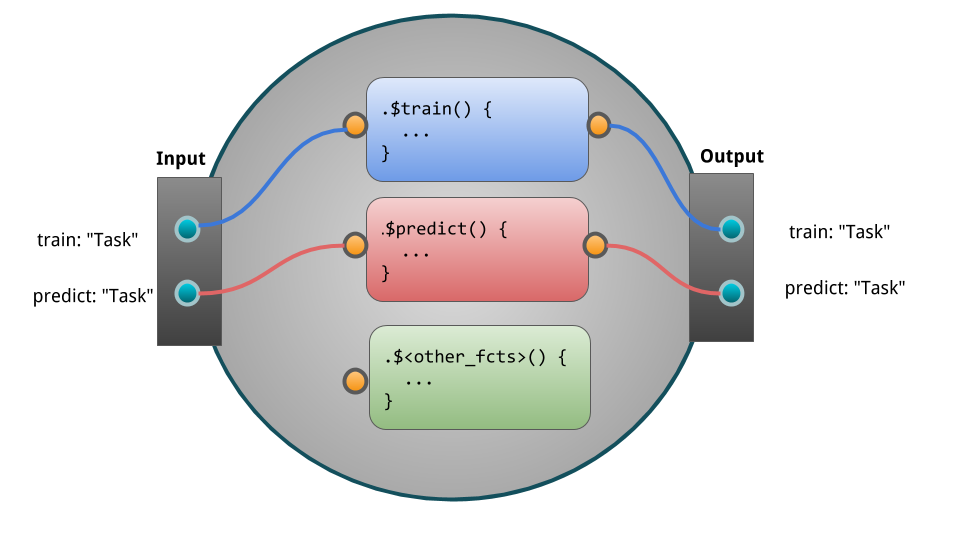
\includegraphics[width=0.9\textwidth,height=\textheight]{images/po_viz.png}
\caption{A PipeOperator}
\end{figure}

\hypertarget{pipe-operator}{%
\section{\texorpdfstring{The Pipeline Operator: \texttt{\%\textgreater{}\textgreater{}\%}}{The Pipeline Operator: \%\textgreater{}\textgreater{}\%}}\label{pipe-operator}}

Although it is possible to create intricate \texttt{Graphs} with edges going all over the place (as long as no loops are introduced), there is usually a clear direction of flow between ``layers'' in the \texttt{Graph}.
It is therefore convenient to build up a \texttt{Graph} from layers.
This can be done using the \textbf{\texttt{\%\textgreater{}\textgreater{}\%}} (``double-arrow'') operator.
It takes either a \texttt{PipeOp} or a \texttt{Graph} on each of its sides and connects all of the outputs of its left-hand side to one of the inputs each of its right-hand side.
The number of inputs therefore must match the number of outputs.

\begin{Shaded}
\begin{Highlighting}[]
\NormalTok{gr =}\StringTok{ }\NormalTok{mlr_pipeops}\OperatorTok{$}\KeywordTok{get}\NormalTok{(}\StringTok{"scale"}\NormalTok{) }\OperatorTok\StringTok{ }\NormalTok{mlr_pipeops}\OperatorTok{$}\KeywordTok{get}\NormalTok{(}\StringTok{"pca"}\NormalTok{)}
\NormalTok{gr}\OperatorTok{$}\KeywordTok{plot}\NormalTok{(}\DataTypeTok{html =} \OtherTok{TRUE}\NormalTok{) }\OperatorTok\StringTok{ }\KeywordTok{visInteraction}\NormalTok{(}\DataTypeTok{zoomView =} \OtherTok{FALSE}\NormalTok{)  }\CommentTok{# disable zoom}
\end{Highlighting}
\end{Shaded}

\begin{center}\includegraphics{mlr3book_files/figure-latex/04-pipelines-008-1} \end{center}

\hypertarget{pipe-nodes-edges-graphs}{%
\section{Nodes, Edges and Graphs}\label{pipe-nodes-edges-graphs}}

POs are combined into \texttt{Graph}s.
The manual way (= hard way) to construct a \texttt{Graph} is to create an empty graph first.
Then one fills the empty graph with POs, and connects edges between the POs.
POs are identified by their \texttt{\$id}.
Note that the operations all modify the object in-place and return the object itself.
Therefore, multiple modifications can be chained.

For this example we use the ``pca'' PO defined above and a new PO named ``mutate''.
The latter creates a new feature from existing variables.

\begin{Shaded}
\begin{Highlighting}[]
\NormalTok{mutate =}\StringTok{ }\NormalTok{mlr_pipeops}\OperatorTok{$}\KeywordTok{get}\NormalTok{(}\StringTok{"mutate"}\NormalTok{)}
\end{Highlighting}
\end{Shaded}

\begin{Shaded}
\begin{Highlighting}[]
\NormalTok{graph =}\StringTok{ }\NormalTok{Graph}\OperatorTok{$}\KeywordTok{new}\NormalTok{()}\OperatorTok{$}\KeywordTok{add_pipeop}\NormalTok{(mutate)}\OperatorTok{$}\KeywordTok{add_pipeop}\NormalTok{(filter)}\OperatorTok{$}\KeywordTok{add_edge}\NormalTok{(}\StringTok{"mutate"}\NormalTok{, }
  \StringTok{"variance"}\NormalTok{)  }\CommentTok{# add connection mutate -> filter}
\end{Highlighting}
\end{Shaded}

The much quicker way is to use the \texttt{\%\textgreater{}\textgreater{}\%} operator to chain POs or \texttt{Graph} s.
The same result as above can be achieved by doing the following:

\begin{Shaded}
\begin{Highlighting}[]
\NormalTok{graph =}\StringTok{ }\NormalTok{mutate }\OperatorTok\StringTok{ }\NormalTok{filter}
\end{Highlighting}
\end{Shaded}

Now the \texttt{Graph} can be inspected using its \texttt{\$plot()} function:

\begin{Shaded}
\begin{Highlighting}[]
\NormalTok{graph}\OperatorTok{$}\KeywordTok{plot}\NormalTok{(}\DataTypeTok{html =} \OtherTok{TRUE}\NormalTok{) }\OperatorTok\StringTok{ }\KeywordTok{visInteraction}\NormalTok{(}\DataTypeTok{zoomView =} \OtherTok{FALSE}\NormalTok{)  }\CommentTok{# disable zoom}
\end{Highlighting}
\end{Shaded}

\begin{center}\includegraphics{mlr3book_files/figure-latex/04-pipelines-012-1} \end{center}

\textbf{Chaining multiple POs of the same kind}

If multiple POs of the same kind should be chained, it is necessary to change the \texttt{id} to avoid name clashes.
This can be done by either accessing the \texttt{\$id} slot or during construction:

\begin{Shaded}
\begin{Highlighting}[]
\NormalTok{graph}\OperatorTok{$}\KeywordTok{add_pipeop}\NormalTok{(mlr_pipeops}\OperatorTok{$}\KeywordTok{get}\NormalTok{(}\StringTok{"pca"}\NormalTok{))}
\end{Highlighting}
\end{Shaded}

\begin{Shaded}
\begin{Highlighting}[]
\NormalTok{graph}\OperatorTok{$}\KeywordTok{add_pipeop}\NormalTok{(mlr_pipeops}\OperatorTok{$}\KeywordTok{get}\NormalTok{(}\StringTok{"pca"}\NormalTok{, }\DataTypeTok{id =} \StringTok{"pca2"}\NormalTok{))}
\end{Highlighting}
\end{Shaded}

\hypertarget{pipe-modeling}{%
\section{Modeling}\label{pipe-modeling}}

The main purpose of a \texttt{Graph} is to build combined preprocessing and model fitting pipelines that can be used as \href{https://mlr3.mlr-org.com}{mlr3} \texttt{Learner}.
In the following we chain two preprocessing tasks:

\begin{itemize}
\tightlist
\item
  mutate (creation of a new feature)
\item
  filter (filtering the dataset)
\end{itemize}

and then chain a PO learner to train and predict on the modified dataset.

\begin{Shaded}
\begin{Highlighting}[]
\NormalTok{graph =}\StringTok{ }\NormalTok{mutate }\OperatorTok\StringTok{ }\NormalTok{filter }\OperatorTok\StringTok{ }\NormalTok{mlr_pipeops}\OperatorTok{$}\KeywordTok{get}\NormalTok{(}\StringTok{"learner"}\NormalTok{, }
  \DataTypeTok{learner =}\NormalTok{ mlr_learners}\OperatorTok{$}\KeywordTok{get}\NormalTok{(}\StringTok{"classif.rpart"}\NormalTok{))}
\end{Highlighting}
\end{Shaded}

Until here we defined the main pipeline stored in \texttt{Graph}.
Now we can train and predict the pipeline:

\begin{Shaded}
\begin{Highlighting}[]
\NormalTok{task =}\StringTok{ }\NormalTok{mlr_tasks}\OperatorTok{$}\KeywordTok{get}\NormalTok{(}\StringTok{"iris"}\NormalTok{)}
\NormalTok{graph}\OperatorTok{$}\KeywordTok{train}\NormalTok{(task)}
\NormalTok{## $classif.rpart.output}
\NormalTok{## NULL}
\NormalTok{graph}\OperatorTok{$}\KeywordTok{predict}\NormalTok{(task)}
\NormalTok{## $classif.rpart.output}
\NormalTok{## <PredictionClassif> for 150 observations:}
\NormalTok{##     row_id     truth  response}
\NormalTok{##          1    setosa    setosa}
\NormalTok{##          2    setosa    setosa}
\NormalTok{##          3    setosa    setosa}
\NormalTok{## ---                           }
\NormalTok{##        148 virginica virginica}
\NormalTok{##        149 virginica virginica}
\NormalTok{##        150 virginica virginica}
\end{Highlighting}
\end{Shaded}

Rather than calling \texttt{\$train()} and \texttt{\$predict()} manually, we can put the pipeline \texttt{Graph} into a \texttt{GraphLearner} object.
A \texttt{GraphLearner} encapsulates the whole pipeline (including the preprocessing steps) and can be put into \texttt{resample()} or \texttt{benchmark()} .
If you are familiar with the old \emph{mlr} package, this is the equivalent of all the \texttt{make*Wrapper()} functions.
The pipeline being encapsulated (here \texttt{Graph} ) must always produce a \texttt{Prediction} with its \texttt{\$predict()} call, so it will probably contain at least one \texttt{PipeOpLearner} .

\begin{Shaded}
\begin{Highlighting}[]
\NormalTok{glrn =}\StringTok{ }\NormalTok{GraphLearner}\OperatorTok{$}\KeywordTok{new}\NormalTok{(graph)}
\end{Highlighting}
\end{Shaded}

This learner can be used for model fitting, resampling, benchmarking, and tuning:

\begin{Shaded}
\begin{Highlighting}[]
\NormalTok{cv3 =}\StringTok{ }\KeywordTok{rsmp}\NormalTok{(}\StringTok{"cv"}\NormalTok{, }\DataTypeTok{folds =} \DecValTok{3}\NormalTok{)}
\KeywordTok{resample}\NormalTok{(task, glrn, cv3)}
\NormalTok{## <ResampleResult> of 3 iterations}
\NormalTok{## * Task: iris}
\NormalTok{## * Learner: mutate.variance.classif.rpart}
\NormalTok{## * Warnings: 0 in 0 iterations}
\NormalTok{## * Errors: 0 in 0 iterations}
\end{Highlighting}
\end{Shaded}

\hypertarget{pipe-hyperpars}{%
\subsection{Setting Hyperparameters}\label{pipe-hyperpars}}

Individual POs offer hyperparameters because they contain \texttt{\$param\_set} slots that can be read and written from \texttt{\$param\_set\$values} (via the paradox package).
The parameters get passed down to the \texttt{Graph}, and finally to the \texttt{GraphLearner} .
This makes it not only possible to easily change the behavior of a \texttt{Graph} / \texttt{GraphLearner} and try different settings manually, but also to perform tuning using the \href{https://mlr3tuning.mlr-org.com}{mlr3tuning} package.

\begin{Shaded}
\begin{Highlighting}[]
\NormalTok{glrn}\OperatorTok{$}\NormalTok{param_set}\OperatorTok{$}\NormalTok{values}\OperatorTok{$}\NormalTok{variance.filter.frac =}\StringTok{ }\FloatTok{0.25}
\NormalTok{cv3 =}\StringTok{ }\KeywordTok{rsmp}\NormalTok{(}\StringTok{"cv"}\NormalTok{, }\DataTypeTok{folds =} \DecValTok{3}\NormalTok{)}
\KeywordTok{resample}\NormalTok{(task, glrn, cv3)}
\NormalTok{## <ResampleResult> of 3 iterations}
\NormalTok{## * Task: iris}
\NormalTok{## * Learner: mutate.variance.classif.rpart}
\NormalTok{## * Warnings: 0 in 0 iterations}
\NormalTok{## * Errors: 0 in 0 iterations}
\end{Highlighting}
\end{Shaded}

\hypertarget{pipe-tuning}{%
\subsection{Tuning}\label{pipe-tuning}}

If you are unfamiliar with tuning in \href{https://mlr3.mlr-org.com}{mlr3}, we recommend to take a look at the section about \protect\hyperlink{tuning}{tuning} first.
Here we define a \texttt{ParamSet} for the ``rpart'' learner and the ``variance'' filter which should be optimized during tuning.

\begin{Shaded}
\begin{Highlighting}[]
\KeywordTok{library}\NormalTok{(}\StringTok{"paradox"}\NormalTok{)}
\NormalTok{ps =}\StringTok{ }\NormalTok{ParamSet}\OperatorTok{$}\KeywordTok{new}\NormalTok{(}\KeywordTok{list}\NormalTok{(ParamDbl}\OperatorTok{$}\KeywordTok{new}\NormalTok{(}\StringTok{"classif.rpart.cp"}\NormalTok{, }\DataTypeTok{lower =} \DecValTok{0}\NormalTok{, }
  \DataTypeTok{upper =} \FloatTok{0.05}\NormalTok{), ParamDbl}\OperatorTok{$}\KeywordTok{new}\NormalTok{(}\StringTok{"variance.filter.frac"}\NormalTok{, }\DataTypeTok{lower =} \FloatTok{0.25}\NormalTok{, }
  \DataTypeTok{upper =} \DecValTok{1}\NormalTok{)))}
\end{Highlighting}
\end{Shaded}

After having defined the \texttt{PerformanceEvaluator}, a random search with 10 iterations is created.
For the inner resampling, we are simply doing holdout (single split into train/test) to keep the runtimes reasonable.

\begin{Shaded}
\begin{Highlighting}[]
\KeywordTok{library}\NormalTok{(}\StringTok{"mlr3tuning"}\NormalTok{)}
\NormalTok{instance =}\StringTok{ }\NormalTok{TuningInstance}\OperatorTok{$}\KeywordTok{new}\NormalTok{(}\DataTypeTok{task =}\NormalTok{ task, }\DataTypeTok{learner =}\NormalTok{ glrn, }
  \DataTypeTok{resampling =} \KeywordTok{rsmp}\NormalTok{(}\StringTok{"holdout"}\NormalTok{), }\DataTypeTok{measures =} \KeywordTok{msr}\NormalTok{(}\StringTok{"classif.ce"}\NormalTok{), }
  \DataTypeTok{param_set =}\NormalTok{ ps, }\DataTypeTok{terminator =} \KeywordTok{term}\NormalTok{(}\StringTok{"evals"}\NormalTok{, }\DataTypeTok{n_evals =} \DecValTok{20}\NormalTok{))}
\end{Highlighting}
\end{Shaded}

\begin{Shaded}
\begin{Highlighting}[]
\NormalTok{tuner =}\StringTok{ }\NormalTok{TunerRandomSearch}\OperatorTok{$}\KeywordTok{new}\NormalTok{()}
\NormalTok{tuner}\OperatorTok{$}\KeywordTok{tune}\NormalTok{(instance)}
\end{Highlighting}
\end{Shaded}

The tuning result can be found in the \texttt{result} slot.

\begin{Shaded}
\begin{Highlighting}[]
\NormalTok{instance}\OperatorTok{$}\NormalTok{result}
\end{Highlighting}
\end{Shaded}

\hypertarget{pipe-nonlinear}{%
\section{Non-Linear Graphs}\label{pipe-nonlinear}}

The Graphs seen so far all have a linear structure.
Some POs may have multiple input or output channels.
These make it possible to create non-linear Graphs with alternative paths taken by the data.

Possible types are:

\begin{itemize}
\tightlist
\item
  \protect\hyperlink{pipe-model-ensembles-branching}{Branching}:
  Splitting of a node into several paths, e.g.~useful when comparing multiple feature-selection methods (pca, filters).
  Only one path will be executed.
\item
  \protect\hyperlink{pipe-model-ensembles-copying}{Copying}:
  Splitting of a node into several paths, all paths will be executed (sequentially).
  Parallel execution is not yet supported.
\item
  \protect\hyperlink{pipe-model-ensembles-stacking}{Stacking}:
  Single graphs are stacked onto each other, i.e.~the output of one \texttt{Graph} is the input for another.
  In machine learning this means that the prediction of one \texttt{Graph} is used as input for another \texttt{Graph}
\end{itemize}

\hypertarget{pipe-model-ensembles-branching-copying}{%
\subsection{Branching \& Copying}\label{pipe-model-ensembles-branching-copying}}

The \texttt{PipeOpBranch} and \texttt{PipeOpUnbranch} POs make it possible to specify multiple alternative paths.
Only one is actually executed, the others are ignored.
The active path is determined by a hyperparameter.
This concept makes it possible to tune alternative preprocessing paths (or learner models).

\texttt{PipeOp(Un)Branch} is initialized either with the number of branches, or with a \texttt{character}-vector indicating the names of the branches.
If names are given, the ``branch-choosing'' hyperparameter becomes more readable.
In the following, we set three options:

\begin{enumerate}
\def\labelenumi{\arabic{enumi}.}
\tightlist
\item
  Doing nothing (``nop'')
\item
  Applying a PCA
\item
  Scaling the data
\end{enumerate}

It is important to ``unbranch'' again after ``branching'', so that the outputs are merged into one result objects.

In the following we first create the branched graph and then show what happens if the ``unbranching'' is not applied:

\begin{Shaded}
\begin{Highlighting}[]
\NormalTok{graph =}\StringTok{ }\NormalTok{mlr_pipeops}\OperatorTok{$}\KeywordTok{get}\NormalTok{(}\StringTok{"branch"}\NormalTok{, }\KeywordTok{c}\NormalTok{(}\StringTok{"nop"}\NormalTok{, }\StringTok{"pca"}\NormalTok{, }\StringTok{"scale"}\NormalTok{)) }\OperatorTok\StringTok{ }
\StringTok{  }\KeywordTok{gunion}\NormalTok{(}\KeywordTok{list}\NormalTok{(mlr_pipeops}\OperatorTok{$}\KeywordTok{get}\NormalTok{(}\StringTok{"nop"}\NormalTok{, }\DataTypeTok{id =} \StringTok{"null1"}\NormalTok{), mlr_pipeops}\OperatorTok{$}\KeywordTok{get}\NormalTok{(}\StringTok{"pca"}\NormalTok{), }
\NormalTok{    mlr_pipeops}\OperatorTok{$}\KeywordTok{get}\NormalTok{(}\StringTok{"scale"}\NormalTok{)))}
\end{Highlighting}
\end{Shaded}

Without ``unbranching'' one creates the following graph:

\begin{Shaded}
\begin{Highlighting}[]
\NormalTok{graph}\OperatorTok{$}\KeywordTok{plot}\NormalTok{(}\DataTypeTok{html =} \OtherTok{TRUE}\NormalTok{) }\OperatorTok\StringTok{ }\KeywordTok{visInteraction}\NormalTok{(}\DataTypeTok{zoomView =} \OtherTok{FALSE}\NormalTok{)  }\CommentTok{# disable zoom}
\end{Highlighting}
\end{Shaded}

\begin{center}\includegraphics{mlr3book_files/figure-latex/04-pipelines-025-1} \end{center}

Now when ``unbranching'', we obtain the following results:

\begin{Shaded}
\begin{Highlighting}[]
\NormalTok{(graph }\OperatorTok\StringTok{ }\NormalTok{mlr_pipeops}\OperatorTok{$}\KeywordTok{get}\NormalTok{(}\StringTok{"unbranch"}\NormalTok{, }\KeywordTok{c}\NormalTok{(}\StringTok{"nop"}\NormalTok{, }\StringTok{"pca"}\NormalTok{, }\StringTok{"scale"}\NormalTok{)))}\OperatorTok{$}\KeywordTok{plot}\NormalTok{(}\DataTypeTok{html =} \OtherTok{TRUE}\NormalTok{) }\OperatorTok\StringTok{ }
\StringTok{  }\KeywordTok{visInteraction}\NormalTok{(}\DataTypeTok{zoomView =} \OtherTok{FALSE}\NormalTok{)  }\CommentTok{# disable zoom}
\end{Highlighting}
\end{Shaded}

\begin{center}\includegraphics{mlr3book_files/figure-latex/04-pipelines-026-1} \end{center}

\hypertarget{pipe-model-ensembles}{%
\subsection{Model Ensembles}\label{pipe-model-ensembles}}

We can leverage the different operations presented to connect POs.
This allows us to form powerful graphs.

Before we go into details, we split the task into train and test indices.

\begin{Shaded}
\begin{Highlighting}[]
\NormalTok{task =}\StringTok{ }\NormalTok{mlr_tasks}\OperatorTok{$}\KeywordTok{get}\NormalTok{(}\StringTok{"iris"}\NormalTok{)}
\NormalTok{train.idx =}\StringTok{ }\KeywordTok{sample}\NormalTok{(}\KeywordTok{seq_len}\NormalTok{(task}\OperatorTok{$}\NormalTok{nrow), }\DecValTok{120}\NormalTok{)}
\NormalTok{test.idx =}\StringTok{ }\KeywordTok{setdiff}\NormalTok{(}\KeywordTok{seq_len}\NormalTok{(task}\OperatorTok{$}\NormalTok{nrow), train.idx)}
\end{Highlighting}
\end{Shaded}

\hypertarget{pipe-model-ensembles-bagging}{%
\subsubsection{Bagging}\label{pipe-model-ensembles-bagging}}

We first examine Bagging introduced by (Breiman \protect\hyperlink{ref-Breiman1996}{1996}).
The basic idea is to create multiple predictors and then aggregate those to a single, more powerful predictor.

\begin{quote}
``\ldots{} multiple versions are formed
by making bootstrap replicates of the learning set
and using these as new learning sets'' (Breiman \protect\hyperlink{ref-Breiman1996}{1996})
\end{quote}

Bagging then aggregates a set of predictors by averaging (regression) or majority vote (classification).
The idea behind bagging is, that a set of weak, but different predictors can be combined in order to arrive at a single, better predictor.

We can achieve this by downsampling our data before training a learner, repeating this e.g.~10 times and then performing a majority vote on the predictions.

First, we create a simple pipeline, that uses \texttt{PipeOpSubsample} before a \texttt{PipeOpLearner} is trained:

\begin{Shaded}
\begin{Highlighting}[]
\NormalTok{single_pred =}\StringTok{ }\NormalTok{PipeOpSubsample}\OperatorTok{$}\KeywordTok{new}\NormalTok{(}\DataTypeTok{param_vals =} \KeywordTok{list}\NormalTok{(}\DataTypeTok{frac =} \FloatTok{0.7}\NormalTok{)) }\OperatorTok\StringTok{ }
\StringTok{  }\NormalTok{PipeOpLearner}\OperatorTok{$}\KeywordTok{new}\NormalTok{(mlr_learners}\OperatorTok{$}\KeywordTok{get}\NormalTok{(}\StringTok{"classif.rpart"}\NormalTok{))}
\end{Highlighting}
\end{Shaded}

We can now copy this operation 10 times using \texttt{greplicate} .

\begin{Shaded}
\begin{Highlighting}[]
\NormalTok{pred_set =}\StringTok{ }\KeywordTok{greplicate}\NormalTok{(single_pred, 10L)}
\end{Highlighting}
\end{Shaded}

Afterwards we need to aggregate the 10 pipelines to form a single model:

\begin{Shaded}
\begin{Highlighting}[]
\NormalTok{bagging =}\StringTok{ }\NormalTok{pred_set }\OperatorTok\StringTok{ }\NormalTok{PipeOpClassifAvg}\OperatorTok{$}\KeywordTok{new}\NormalTok{(}\DataTypeTok{innum =}\NormalTok{ 10L)}
\end{Highlighting}
\end{Shaded}

Now we can plot again to see what happens:

\begin{Shaded}
\begin{Highlighting}[]
\NormalTok{vn =}\StringTok{ }\NormalTok{bagging}\OperatorTok{$}\KeywordTok{plot}\NormalTok{(}\DataTypeTok{html =} \OtherTok{TRUE}\NormalTok{)}
\NormalTok{visNetwork}\OperatorTok{::}\KeywordTok{visInteraction}\NormalTok{(vn, }\DataTypeTok{zoomView =} \OtherTok{FALSE}\NormalTok{)  }\CommentTok{# disable zoom}
\end{Highlighting}
\end{Shaded}

\begin{center}\includegraphics{mlr3book_files/figure-latex/04-pipelines-031-1} \end{center}

This pipeline can again be used in conjunction with \texttt{GraphLearner} in order for Bagging to be used like a \texttt{Learner}:

\begin{Shaded}
\begin{Highlighting}[]
\NormalTok{baglrn =}\StringTok{ }\NormalTok{GraphLearner}\OperatorTok{$}\KeywordTok{new}\NormalTok{(bagging)}
\NormalTok{baglrn}\OperatorTok{$}\KeywordTok{train}\NormalTok{(task, train.idx)}
\NormalTok{baglrn}\OperatorTok{$}\KeywordTok{predict}\NormalTok{(task, test.idx)}
\NormalTok{## <PredictionClassif> for 30 observations:}
\NormalTok{##     row_id     truth  response}
\NormalTok{##          2    setosa    setosa}
\NormalTok{##          5    setosa    setosa}
\NormalTok{##         12    setosa    setosa}
\NormalTok{## ---                           }
\NormalTok{##        144 virginica virginica}
\NormalTok{##        145 virginica virginica}
\NormalTok{##        147 virginica virginica}
\end{Highlighting}
\end{Shaded}

In conjunction with different \texttt{Backends}, this can be a very powerful tool.
In cases when the data does not fully fit in memory, one can obtain a fraction of the data for each learner from a \texttt{DataBackend} and then aggregate predictions over all learners.

\hypertarget{pipe-model-ensembles-stacking}{%
\subsubsection{Stacking}\label{pipe-model-ensembles-stacking}}

Stacking (Wolpert \protect\hyperlink{ref-Wolpert1992}{1992}) is another technique that can improve model performance.
The basic idea behind stacking is the use of predictions from one model as features for a subsequent model to possibly improve performance.

As an example we can train a decision tree and use the predictions from this model in conjunction with the original features in order to train an additional model on top.

To limit overfitting, we additionally do not predict on the original predictions of the learner.
Instead, we predict on out-of-bag predictions.
To do all this, we can use \texttt{PipeOpLearnerCV} .

\texttt{PipeOpLearnerCV} performs nested cross-validation on the training data, fitting a model in each fold.
Each of the models is then used to predict on the out-of-fold data.
As a result, we obtain predictions for every data point in our input data.

We first create a ``level 0'' learner, which is used to extract a lower level prediction.
Additionally, we \texttt{clone()} the learner object to obtain a copy of the learner.
Subsequently, one sets a custom id for the \texttt{PipeOp} .

\begin{Shaded}
\begin{Highlighting}[]
\NormalTok{lrn =}\StringTok{ }\NormalTok{mlr_learners}\OperatorTok{$}\KeywordTok{get}\NormalTok{(}\StringTok{"classif.rpart"}\NormalTok{)}
\NormalTok{lrn_}\DecValTok{0}\NormalTok{ =}\StringTok{ }\NormalTok{PipeOpLearnerCV}\OperatorTok{$}\KeywordTok{new}\NormalTok{(lrn}\OperatorTok{$}\KeywordTok{clone}\NormalTok{())}
\NormalTok{lrn_}\DecValTok{0}\OperatorTok{$}\NormalTok{id =}\StringTok{ "rpart_cv"}
\end{Highlighting}
\end{Shaded}

We use a `FIXME' in parallel to the ``level 0'' learner, in order to send the unchanged Task to the next level, where it is then combined with the predictions from our decision tree learner.

\begin{Shaded}
\begin{Highlighting}[]
\NormalTok{level_}\DecValTok{0}\NormalTok{ =}\StringTok{ }\KeywordTok{gunion}\NormalTok{(}\KeywordTok{list}\NormalTok{(lrn_}\DecValTok{0}\NormalTok{, PipeOpNOP}\OperatorTok{$}\KeywordTok{new}\NormalTok{()))}
\end{Highlighting}
\end{Shaded}

Afterwards, we want to concatenate the predictions from \texttt{PipeOpLearnerCV} and the original Task using \texttt{PipeOpFeatureUnion} :

\begin{Shaded}
\begin{Highlighting}[]
\NormalTok{combined =}\StringTok{ }\NormalTok{level_}\DecValTok{0} \OperatorTok\StringTok{ }\NormalTok{PipeOpFeatureUnion}\OperatorTok{$}\KeywordTok{new}\NormalTok{(}\DecValTok{2}\NormalTok{)}
\end{Highlighting}
\end{Shaded}

Now we can train another learner on top of the combined features:

\begin{Shaded}
\begin{Highlighting}[]
\NormalTok{stack =}\StringTok{ }\NormalTok{combined }\OperatorTok\StringTok{ }\NormalTok{PipeOpLearner}\OperatorTok{$}\KeywordTok{new}\NormalTok{(lrn}\OperatorTok{$}\KeywordTok{clone}\NormalTok{())}
\NormalTok{vn =}\StringTok{ }\NormalTok{stack}\OperatorTok{$}\KeywordTok{plot}\NormalTok{(}\DataTypeTok{html =} \OtherTok{TRUE}\NormalTok{)}
\NormalTok{visNetwork}\OperatorTok{::}\KeywordTok{visInteraction}\NormalTok{(vn, }\DataTypeTok{zoomView =} \OtherTok{FALSE}\NormalTok{)  }\CommentTok{# disable zoom}
\end{Highlighting}
\end{Shaded}

\begin{Shaded}
\begin{Highlighting}[]
\NormalTok{stacklrn =}\StringTok{ }\NormalTok{GraphLearner}\OperatorTok{$}\KeywordTok{new}\NormalTok{(stack)}
\NormalTok{stacklrn}\OperatorTok{$}\KeywordTok{train}\NormalTok{(task, train.idx)}
\NormalTok{stacklrn}\OperatorTok{$}\KeywordTok{predict}\NormalTok{(task, test.idx)}
\end{Highlighting}
\end{Shaded}

In this vignette, we showed a very simple usecase for stacking.
In many real-world applications, stacking is done for multiple levels and on multiple representations of the dataset.
On a lower level, different preprocessing methods can be defined in conjunction with several learners.
On a higher level, we can then combine those predictions in order to form a very powerful model.

\hypertarget{multilevel-stacking}{%
\subsubsection{Multilevel Stacking}\label{multilevel-stacking}}

In order to showcase the power of \href{https://mlr3pipelines.mlr-org.com}{mlr3pipelines}, we will show a more complicated stacking example.

In this case, we train a \texttt{glmnet} and 2 different \texttt{rpart} models (some transform its inputs using \texttt{PipeOpPCA} ) on our task in the ``level 0'' and concatenate them with the original features (via `FIXME').
The result is then passed on to ``level 1'', where we copy the concatenated features 3 times and put this task into an \texttt{rpart} and a \texttt{glmnet} model.
Additionally, we keep a version of the ``level 0'' output (via `FIXME') and pass this on to ``level 2''.
In ``level 2'' we simply concatenate all ``level 1'' outputs and train a final decision tree.

\begin{Shaded}
\begin{Highlighting}[]
\KeywordTok{library}\NormalTok{(mlr3learners)  }\CommentTok{# for classif.glmnet}
\NormalTok{rprt =}\StringTok{ }\KeywordTok{lrn}\NormalTok{(}\StringTok{"classif.rpart"}\NormalTok{, }\DataTypeTok{predict_type =} \StringTok{"prob"}\NormalTok{)}
\NormalTok{glmn =}\StringTok{ }\KeywordTok{lrn}\NormalTok{(}\StringTok{"classif.glmnet"}\NormalTok{, }\DataTypeTok{predict_type =} \StringTok{"prob"}\NormalTok{)}

\CommentTok{# Create Learner CV Operators}
\NormalTok{lrn_}\DecValTok{0}\NormalTok{ =}\StringTok{ }\NormalTok{PipeOpLearnerCV}\OperatorTok{$}\KeywordTok{new}\NormalTok{(rprt, }\DataTypeTok{id =} \StringTok{"rpart_cv_1"}\NormalTok{)}
\NormalTok{lrn_}\DecValTok{0}\OperatorTok{$}\NormalTok{values}\OperatorTok{$}\NormalTok{maxdepth =}\StringTok{ }\NormalTok{5L}
\NormalTok{lrn_}\DecValTok{1}\NormalTok{ =}\StringTok{ }\NormalTok{PipeOpPCA}\OperatorTok{$}\KeywordTok{new}\NormalTok{(}\DataTypeTok{id =} \StringTok{"pca1"}\NormalTok{) }\OperatorTok\StringTok{ }\NormalTok{PipeOpLearnerCV}\OperatorTok{$}\KeywordTok{new}\NormalTok{(rprt, }
  \DataTypeTok{id =} \StringTok{"rpart_cv_2"}\NormalTok{)}
\NormalTok{lrn_}\DecValTok{1}\OperatorTok{$}\NormalTok{values}\OperatorTok{$}\NormalTok{rpart_cv_}\FloatTok{2.}\NormalTok{maxdepth =}\StringTok{ }\NormalTok{1L}
\NormalTok{lrn_}\DecValTok{2}\NormalTok{ =}\StringTok{ }\NormalTok{PipeOpPCA}\OperatorTok{$}\KeywordTok{new}\NormalTok{(}\DataTypeTok{id =} \StringTok{"pca2"}\NormalTok{) }\OperatorTok\StringTok{ }\NormalTok{PipeOpLearnerCV}\OperatorTok{$}\KeywordTok{new}\NormalTok{(glmn)}

\CommentTok{# Union them with a PipeOpNULL to keep original features}
\NormalTok{level_}\DecValTok{0}\NormalTok{ =}\StringTok{ }\KeywordTok{gunion}\NormalTok{(}\KeywordTok{list}\NormalTok{(lrn_}\DecValTok{0}\NormalTok{, lrn_}\DecValTok{1}\NormalTok{, lrn_}\DecValTok{2}\NormalTok{, PipeOpNOP}\OperatorTok{$}\KeywordTok{new}\NormalTok{(}\DataTypeTok{id =} \StringTok{"NOP1"}\NormalTok{)))}

\CommentTok{# Cbind the output 3 times, train 2 learners but also}
\CommentTok{# keep level 0 predictions}
\NormalTok{level_}\DecValTok{1}\NormalTok{ =}\StringTok{ }\NormalTok{level_}\DecValTok{0} \OperatorTok\StringTok{ }\NormalTok{PipeOpFeatureUnion}\OperatorTok{$}\KeywordTok{new}\NormalTok{(}\DecValTok{4}\NormalTok{) }\OperatorTok\StringTok{ }\NormalTok{PipeOpCopy}\OperatorTok{$}\KeywordTok{new}\NormalTok{(}\DecValTok{3}\NormalTok{) }\OperatorTok\StringTok{ }
\StringTok{  }\KeywordTok{gunion}\NormalTok{(}\KeywordTok{list}\NormalTok{(PipeOpLearnerCV}\OperatorTok{$}\KeywordTok{new}\NormalTok{(rprt, }\DataTypeTok{id =} \StringTok{"rpart_cv_l1"}\NormalTok{), }
\NormalTok{    PipeOpLearnerCV}\OperatorTok{$}\KeywordTok{new}\NormalTok{(glmn, }\DataTypeTok{id =} \StringTok{"glmnt_cv_l1"}\NormalTok{), PipeOpNOP}\OperatorTok{$}\KeywordTok{new}\NormalTok{(}\DataTypeTok{id =} \StringTok{"NOP_l1"}\NormalTok{)))}

\CommentTok{# Cbind predictions, train a final learner}
\NormalTok{level_}\DecValTok{2}\NormalTok{ =}\StringTok{ }\NormalTok{level_}\DecValTok{1} \OperatorTok\StringTok{ }\NormalTok{PipeOpFeatureUnion}\OperatorTok{$}\KeywordTok{new}\NormalTok{(}\DecValTok{3}\NormalTok{, }\DataTypeTok{id =} \StringTok{"u2"}\NormalTok{) }\OperatorTok\StringTok{ }
\StringTok{  }\NormalTok{PipeOpLearner}\OperatorTok{$}\KeywordTok{new}\NormalTok{(rprt, }\DataTypeTok{id =} \StringTok{"rpart_l2"}\NormalTok{)}

\CommentTok{# Plot the resulting graph}
\NormalTok{vn =}\StringTok{ }\NormalTok{level_}\DecValTok{2}\OperatorTok{$}\KeywordTok{plot}\NormalTok{(}\DataTypeTok{html =} \OtherTok{TRUE}\NormalTok{)}
\NormalTok{visNetwork}\OperatorTok{::}\KeywordTok{visInteraction}\NormalTok{(vn, }\DataTypeTok{zoomView =} \OtherTok{FALSE}\NormalTok{)  }\CommentTok{# disable zoom}

\NormalTok{task =}\StringTok{ }\KeywordTok{tsk}\NormalTok{(}\StringTok{"iris"}\NormalTok{)}
\NormalTok{lrn =}\StringTok{ }\NormalTok{GraphLearner}\OperatorTok{$}\KeywordTok{new}\NormalTok{(level_}\DecValTok{2}\NormalTok{)}

\NormalTok{lrn}\OperatorTok{$}\KeywordTok{train}\NormalTok{(task, train.idx)}\OperatorTok{$}\KeywordTok{predict}\NormalTok{(task, test.idx)}\OperatorTok{$}\KeywordTok{score}\NormalTok{()}
\end{Highlighting}
\end{Shaded}

\hypertarget{pipe-special-ops}{%
\section{Special Operators}\label{pipe-special-ops}}

This section introduces some special operators, that might be useful in many applications.

\hypertarget{imputation-pipeopimpute}{%
\subsection{\texorpdfstring{Imputation: \texttt{PipeOpImpute}}{Imputation: PipeOpImpute}}\label{imputation-pipeopimpute}}

An often occurring setting is the imputation of missing data.
Imputation methods range from relatively simple imputation using either \emph{mean}, \emph{median} or histograms to way more involved methods including using machine learning algorithms in order to predict missing values.

The following \texttt{PipeOp}, \texttt{PipeOpImpute}, imputes numeric values from a histogram, adds a new level for factors and additionally adds a column marking whether a value for a given feature was missing or not.

\begin{Shaded}
\begin{Highlighting}[]
\NormalTok{pom =}\StringTok{ }\NormalTok{PipeOpMissInd}\OperatorTok{$}\KeywordTok{new}\NormalTok{()}
\NormalTok{pon =}\StringTok{ }\NormalTok{PipeOpImputeHist}\OperatorTok{$}\KeywordTok{new}\NormalTok{(}\DataTypeTok{id =} \StringTok{"imputer_num"}\NormalTok{, }\DataTypeTok{param_vals =} \KeywordTok{list}\NormalTok{(}\DataTypeTok{affect_columns =}\NormalTok{ is.numeric))}
\NormalTok{pof =}\StringTok{ }\NormalTok{PipeOpImputeNewlvl}\OperatorTok{$}\KeywordTok{new}\NormalTok{(}\DataTypeTok{id =} \StringTok{"imputer_fct"}\NormalTok{, }\DataTypeTok{param_vals =} \KeywordTok{list}\NormalTok{(}\DataTypeTok{affect_columns =}\NormalTok{ is.factor))}
\NormalTok{imputer =}\StringTok{ }\NormalTok{pom }\OperatorTok\StringTok{ }\NormalTok{pon }\OperatorTok\StringTok{ }\NormalTok{pof}
\end{Highlighting}
\end{Shaded}

A learner can thus be equipped with automatic imputation of missing values by adding an imputation Pipeop.

\begin{Shaded}
\begin{Highlighting}[]
\NormalTok{polrn =}\StringTok{ }\NormalTok{PipeOpLearner}\OperatorTok{$}\KeywordTok{new}\NormalTok{(mlr_learners}\OperatorTok{$}\KeywordTok{get}\NormalTok{(}\StringTok{"classif.rpart"}\NormalTok{))}
\NormalTok{lrn =}\StringTok{ }\NormalTok{GraphLearner}\OperatorTok{$}\KeywordTok{new}\NormalTok{(}\DataTypeTok{graph =}\NormalTok{ imputer }\OperatorTok\StringTok{ }\NormalTok{polrn)}
\end{Highlighting}
\end{Shaded}

\hypertarget{feature-engineering-pipeopmutate}{%
\subsection{\texorpdfstring{Feature Engineering: \texttt{PipeOpMutate}}{Feature Engineering: PipeOpMutate}}\label{feature-engineering-pipeopmutate}}

New features can be added or computed from a task using \texttt{PipeOpMutate} .
The operator evaluates one or multiple expressions provided in an \texttt{alist}.
In this example, we compute some new features on top of the \texttt{iris} task.
Then we add them to the data as illustrated below:

\begin{Shaded}
\begin{Highlighting}[]
\NormalTok{pom =}\StringTok{ }\NormalTok{PipeOpMutate}\OperatorTok{$}\KeywordTok{new}\NormalTok{()}

\CommentTok{# Define a set of mutations}
\NormalTok{mutations =}\StringTok{ }\KeywordTok{list}\NormalTok{(}\DataTypeTok{Sepal.Sum =} \OperatorTok{~}\NormalTok{Sepal.Length }\OperatorTok{+}\StringTok{ }\NormalTok{Sepal.Width, }
  \DataTypeTok{Petal.Sum =} \OperatorTok{~}\NormalTok{Petal.Length }\OperatorTok{+}\StringTok{ }\NormalTok{Petal.Width, }\DataTypeTok{Sepal.Petal.Ratio =} \OperatorTok{~}\NormalTok{(Sepal.Length}\OperatorTok{/}\NormalTok{Petal.Length))}
\NormalTok{pom}\OperatorTok{$}\NormalTok{param_set}\OperatorTok{$}\NormalTok{values}\OperatorTok{$}\NormalTok{mutation =}\StringTok{ }\NormalTok{mutations}
\end{Highlighting}
\end{Shaded}

If outside data is required, we can make use of the \texttt{env} parameter.
Moreover, we provide an environment, where expressions are evaluated (\texttt{env} defaults to \texttt{.GlobalEnv}).

\hypertarget{training-on-data-subsets-pipeopchunk}{%
\subsection{\texorpdfstring{Training on data subsets: \texttt{PipeOpChunk}}{Training on data subsets: PipeOpChunk}}\label{training-on-data-subsets-pipeopchunk}}

In cases, where data is too big to fit into the machine's memory, an often-used technique is to split the data into several parts.
Subsequently, the parts are trained on each part of the data.
After undertaking these steps, we aggregate the models.
In this example, we split our data into 4 parts using \texttt{PipeOpChunk} .
Additionally, we create 4 \texttt{PipeOpLearner} POS, which are then trained on each split of the data.

\begin{Shaded}
\begin{Highlighting}[]
\NormalTok{chks =}\StringTok{ }\NormalTok{PipeOpChunk}\OperatorTok{$}\KeywordTok{new}\NormalTok{(}\DecValTok{4}\NormalTok{)}
\NormalTok{lrns =}\StringTok{ }\KeywordTok{greplicate}\NormalTok{(PipeOpLearner}\OperatorTok{$}\KeywordTok{new}\NormalTok{(mlr_learners}\OperatorTok{$}\KeywordTok{get}\NormalTok{(}\StringTok{"classif.rpart"}\NormalTok{)), }
  \DecValTok{4}\NormalTok{)}
\end{Highlighting}
\end{Shaded}

Afterwards we can use \texttt{PipeOpClassifAvg} to aggregate the predictions from the 4 different models into a new one.

\begin{Shaded}
\begin{Highlighting}[]
\NormalTok{mjv =}\StringTok{ }\NormalTok{PipeOpClassifAvg}\OperatorTok{$}\KeywordTok{new}\NormalTok{(}\DecValTok{4}\NormalTok{)}
\end{Highlighting}
\end{Shaded}

We can now connect the different operators and visualize the full graph:

\begin{Shaded}
\begin{Highlighting}[]
\NormalTok{pipeline =}\StringTok{ }\NormalTok{chks }\OperatorTok\StringTok{ }\NormalTok{lrns }\OperatorTok\StringTok{ }\NormalTok{mjv}
\NormalTok{pipeline}\OperatorTok{$}\KeywordTok{plot}\NormalTok{(}\DataTypeTok{html =} \OtherTok{TRUE}\NormalTok{) }\OperatorTok\StringTok{ }\KeywordTok{visInteraction}\NormalTok{(}\DataTypeTok{zoomView =} \OtherTok{FALSE}\NormalTok{)  }\CommentTok{# disable zoom}
\end{Highlighting}
\end{Shaded}

\begin{center}\includegraphics{mlr3book_files/figure-latex/04-pipelines-044-1} \end{center}

\begin{Shaded}
\begin{Highlighting}[]
\NormalTok{pipelrn =}\StringTok{ }\NormalTok{GraphLearner}\OperatorTok{$}\KeywordTok{new}\NormalTok{(pipeline)}
\NormalTok{pipelrn}\OperatorTok{$}\KeywordTok{train}\NormalTok{(task, train.idx)}\OperatorTok{$}\KeywordTok{predict}\NormalTok{(task, train.idx)}\OperatorTok{$}\KeywordTok{score}\NormalTok{()}
\NormalTok{## classif.ce }
\NormalTok{##      0.025}
\end{Highlighting}
\end{Shaded}

\hypertarget{feature-selection-pipeopfilter-and-pipeopselect}{%
\subsection{\texorpdfstring{Feature Selection: \texttt{PipeOpFilter} and \texttt{PipeOpSelect}}{Feature Selection: PipeOpFilter and PipeOpSelect}}\label{feature-selection-pipeopfilter-and-pipeopselect}}

The package \href{https://mlr3filters.mlr-org.com}{mlr3filters} contains many different \texttt{mlr3filters::Filter}s that can be used to select features for subsequent learners.
This is often required when the data has a large amount of features.

A \texttt{PipeOp} for filters is \texttt{PipeOpFilter}:

\begin{Shaded}
\begin{Highlighting}[]
\NormalTok{PipeOpFilter}\OperatorTok{$}\KeywordTok{new}\NormalTok{(mlr3filters}\OperatorTok{::}\NormalTok{FilterInformationGain}\OperatorTok{$}\KeywordTok{new}\NormalTok{())}
\NormalTok{## PipeOp: <information_gain> (not trained)}
\NormalTok{## values: <list()>}
\NormalTok{## Input channels <name [train type, predict type]>:}
\NormalTok{##   input [Task,Task]}
\NormalTok{## Output channels <name [train type, predict type]>:}
\NormalTok{##   output [Task,Task]}
\end{Highlighting}
\end{Shaded}

How many features to keep can be set using \texttt{filter\_nfeat}, \texttt{filter\_frac} and \texttt{filter\_cutoff}.

Filters can be selected / de-selected by name using \texttt{PipeOpSelect} .

\hypertarget{technical}{%
\chapter{Technical}\label{technical}}

This chapter provides an overview of technical details of the \href{https://mlr3.mlr-org.com}{mlr3} framework.

\textbf{Parallelization}

At first, some details about \protect\hyperlink{parallelization}{Parallelization} and the usage of the \texttt{future} are given.
Parallelization refers to the process of running multiple jobs simultaneously.
This process is employed to minimize the necessary computing power.
Algorithms consist of both sequential (non-parallelizable) and parallelizable parts.
Therefore, parallelization does not always alter performance in a positive substantial manner.
Summed up, this sub-chapter illustrates how and when to use parallelization in mlr3.

\textbf{Database Backends}

The section \protect\hyperlink{backends}{Database Backends} describes how to work with database backends that \href{https://mlr3.mlr-org.com}{mlr3} supports.
Database backends can be helpful for large data processing which does not fit in memory or is stored natively in a database (e.g.~SQLite).
Specifically when working with large data sets, or when undertaking numerous tasks simultaneously, it can be advantageous to interface out-of-memory data.
The section provides an illustration of how to implement \protect\hyperlink{backends}{Database Backends} using of NYC flight data.

\textbf{Parameters}

In the section \protect\hyperlink{paradox}{Parameters} instructions are given on how to:

\begin{itemize}
\tightlist
\item
  define parameter sets for learners
\item
  undertake parameter sampling
\item
  apply parameter transformations
\end{itemize}

For illustrative purposes, this sub-chapter uses the \href{https://paradox.mlr-org.com}{paradox} package, the successor of \texttt{ParamHelpers}.

\textbf{Logging and Verbosity}

The sub-chapter on \protect\hyperlink{logging}{Logging and Verbosity} shows how to change the most important settings related to logging.
In \emph{mlr3} we use the \emph{lgr} package.

\textbf{Transition Guide}

Lastly, we provide a \protect\hyperlink{transition}{Transition Guide} for users of the old \texttt{mlr} who want to switch to \href{https://mlr3.mlr-org.com}{mlr3}.

\hypertarget{parallelization}{%
\section{Parallelization}\label{parallelization}}

Parallelization refers to the process of running multiple jobs in parallel, simultaneously.
This process allows for significant savings in computing power.

\texttt{mlr-org/mlr3} uses the \texttt{future} backends for parallelization.
Make sure you have installed the required packages \texttt{future} and \texttt{future.apply}:

\texttt{mlr-org/mlr3} is capable of parallelizing a variety of different scenarios.
One of the most used cases is to parallelize the \texttt{Resampling} iterations.
See \protect\hyperlink{resampling}{Section Resampling} for a detailed introduction to resampling.

In the following section, we will use the \emph{spam} task and a simple classification tree (\texttt{"classif.rpart"}) to showcase parallelization.
We use the \texttt{future} package to parallelize the resampling by selecting a backend via the function \texttt{future::plan()}.
We use the \texttt{"multiprocess"} backend here which uses threads on UNIX based systems and a ``Socket'' cluster on Windows.

\begin{Shaded}
\begin{Highlighting}[]
\NormalTok{future}\OperatorTok{::}\KeywordTok{plan}\NormalTok{(}\StringTok{"multiprocess"}\NormalTok{)}

\NormalTok{task =}\StringTok{ }\KeywordTok{tsk}\NormalTok{(}\StringTok{"spam"}\NormalTok{)}
\NormalTok{learner =}\StringTok{ }\KeywordTok{lrn}\NormalTok{(}\StringTok{"classif.rpart"}\NormalTok{)}
\NormalTok{resampling =}\StringTok{ }\KeywordTok{rsmp}\NormalTok{(}\StringTok{"subsampling"}\NormalTok{)}

\NormalTok{time =}\StringTok{ }\KeywordTok{Sys.time}\NormalTok{()}
\KeywordTok{resample}\NormalTok{(task, learner, resampling)}
\KeywordTok{Sys.time}\NormalTok{() }\OperatorTok{-}\StringTok{ }\NormalTok{time}
\end{Highlighting}
\end{Shaded}

\begin{caution}
By default all CPUs of your machine are used unless you specify argument
\texttt{workers} in \texttt{future::plan()}.
\end{caution}

On most systems you should see a decrease in the reported elapsed time.
On some systems (e.g.~Windows), the overhead for parallelization is quite large though.
Therefore, it is advised to only enable parallelization for resamplings where each iteration runs at least 10s.

\textbf{Choosing the parallelization level}

If you are transitioning from \texttt{mlr}, you might be used to selecting different parallelization levels, e.g.~for resampling, benchmarking or tuning.
In \texttt{mlr-org/mlr3} this is no longer required.
All kind of events are rolled out on the same level.
Therefore, there is no need to decide whether you want to parallelize the tuning OR the resampling.

In \texttt{mlr-org/mlr3} this is no longer required.
All kind of events are rolled out on the same level - there is no need to decide whether you want to parallelize the tuning OR the resampling.

Just lean back and let the machine do the work :-)

\hypertarget{error-handling}{%
\section{Error Handling}\label{error-handling}}

To demonstrate how to properly deal with misbehaving learners, \texttt{mlr-org/mlr3} ships with the learner \texttt{mlr\_learners\_classif.debug",\ "classif.debug}:

\begin{Shaded}
\begin{Highlighting}[]
\NormalTok{task =}\StringTok{ }\KeywordTok{tsk}\NormalTok{(}\StringTok{"iris"}\NormalTok{)}
\NormalTok{learner =}\StringTok{ }\KeywordTok{lrn}\NormalTok{(}\StringTok{"classif.debug"}\NormalTok{)}
\KeywordTok{print}\NormalTok{(learner)}
\NormalTok{## <LearnerClassifDebug:classif.debug>}
\NormalTok{## * Model: -}
\NormalTok{## * Parameters: list()}
\NormalTok{## * Packages: -}
\NormalTok{## * Predict Type: response}
\NormalTok{## * Feature types: logical, integer, numeric,}
\NormalTok{##   character, factor, ordered}
\NormalTok{## * Properties: missings, multiclass, twoclass}
\end{Highlighting}
\end{Shaded}

This learner comes with special hyperparameters that let us control

\begin{enumerate}
\def\labelenumi{\arabic{enumi}.}
\tightlist
\item
  what conditions should be signaled (message, warning, error, segfault) with what probability,
\item
  during which stage the conditions should be signaled (train or predict), and
\item
  the ratio of predictions being \texttt{NA} (\texttt{predict\_missing}).
\end{enumerate}

\begin{Shaded}
\begin{Highlighting}[]
\NormalTok{learner}\OperatorTok{$}\NormalTok{param_set}
\NormalTok{## ParamSet: }
\NormalTok{##                   id    class lower upper      levels}
\NormalTok{##  1:    message_train ParamDbl     0     1            }
\NormalTok{##  2:  message_predict ParamDbl     0     1            }
\NormalTok{##  3:    warning_train ParamDbl     0     1            }
\NormalTok{##  4:  warning_predict ParamDbl     0     1            }
\NormalTok{##  5:      error_train ParamDbl     0     1            }
\NormalTok{##  6:    error_predict ParamDbl     0     1            }
\NormalTok{##  7:   segfault_train ParamDbl     0     1            }
\NormalTok{##  8: segfault_predict ParamDbl     0     1            }
\NormalTok{##  9:  predict_missing ParamDbl     0     1            }
\NormalTok{## 10:       save_tasks ParamLgl    NA    NA  TRUE,FALSE}
\NormalTok{## 11:                x ParamDbl     0     1            }
\NormalTok{##         default value}
\NormalTok{##  1:           0      }
\NormalTok{##  2:           0      }
\NormalTok{##  3:           0      }
\NormalTok{##  4:           0      }
\NormalTok{##  5:           0      }
\NormalTok{##  6:           0      }
\NormalTok{##  7:           0      }
\NormalTok{##  8:           0      }
\NormalTok{##  9:           0      }
\NormalTok{## 10:       FALSE      }
\NormalTok{## 11: <NoDefault>}
\end{Highlighting}
\end{Shaded}

With the learner's default settings, the learner will do nothing special: The learner learns a random label and creates constant predictions.

\begin{Shaded}
\begin{Highlighting}[]
\NormalTok{task =}\StringTok{ }\KeywordTok{tsk}\NormalTok{(}\StringTok{"iris"}\NormalTok{)}
\NormalTok{learner}\OperatorTok{$}\KeywordTok{train}\NormalTok{(task)}\OperatorTok{$}\KeywordTok{predict}\NormalTok{(task)}\OperatorTok{$}\NormalTok{confusion}
\NormalTok{##             truth}
\NormalTok{## response     setosa versicolor virginica}
\NormalTok{##   setosa         50         50        50}
\NormalTok{##   versicolor      0          0         0}
\NormalTok{##   virginica       0          0         0}
\end{Highlighting}
\end{Shaded}

We now set a hyperparameter to let the debug learner signal an error during the train step.
By default,\texttt{mlr-org/mlr3} does not catch conditions such as warnings or errors raised by third-party code like learners:

\begin{Shaded}
\begin{Highlighting}[]
\NormalTok{learner}\OperatorTok{$}\NormalTok{param_set}\OperatorTok{$}\NormalTok{values =}\StringTok{ }\KeywordTok{list}\NormalTok{(}\DataTypeTok{error_train =} \DecValTok{1}\NormalTok{)}
\NormalTok{learner}\OperatorTok{$}\KeywordTok{train}\NormalTok{(}\KeywordTok{tsk}\NormalTok{(}\StringTok{"iris"}\NormalTok{))}
\NormalTok{## Error in learner$train_internal(task = task): Error from classif.debug->train()}
\end{Highlighting}
\end{Shaded}

If this would be a regular learner, we could now start debugging with \texttt{traceback()} (or create a \href{https://stackoverflow.com/help/minimal-reproducible-example}{MRE} to file a bug report).

However, machine learning algorithms raising errors is not uncommon as algorithms typically cannot process all possible data.
Thus, we need a mechanism to

\begin{enumerate}
\def\labelenumi{\arabic{enumi}.}
\tightlist
\item
  capture all signaled conditions such as messages, warnings and errors so that we can analyze them post-hoc, and
\item
  a statistically sound way to proceed the calculation and be able to aggregate over partial results.
\end{enumerate}

These two mechanisms are explained in the following subsections.

\hypertarget{encapsulation}{%
\subsection{Encapsulation}\label{encapsulation}}

With encapsulation, exceptions do not stop the program flow and all output is logged to the learner (instead of printed to the console).
Each \texttt{Learner} has a field \texttt{encapsulate} to control how the train or predict steps are executed.
One way to encapsulate the execution is provided by the package \texttt{evaluate} (see \texttt{encapsulate()} for more details):

\begin{Shaded}
\begin{Highlighting}[]
\NormalTok{task =}\StringTok{ }\KeywordTok{tsk}\NormalTok{(}\StringTok{"iris"}\NormalTok{)}
\NormalTok{learner =}\StringTok{ }\KeywordTok{lrn}\NormalTok{(}\StringTok{"classif.debug"}\NormalTok{)}
\NormalTok{learner}\OperatorTok{$}\NormalTok{param_set}\OperatorTok{$}\NormalTok{values =}\StringTok{ }\KeywordTok{list}\NormalTok{(}\DataTypeTok{warning_train =} \DecValTok{1}\NormalTok{, }\DataTypeTok{error_train =} \DecValTok{1}\NormalTok{)}
\NormalTok{learner}\OperatorTok{$}\NormalTok{encapsulate =}\StringTok{ }\KeywordTok{c}\NormalTok{(}\DataTypeTok{train =} \StringTok{"evaluate"}\NormalTok{, }\DataTypeTok{predict =} \StringTok{"evaluate"}\NormalTok{)}

\NormalTok{learner}\OperatorTok{$}\KeywordTok{train}\NormalTok{(task)}
\end{Highlighting}
\end{Shaded}

After training the learner, one can access the recorded log via the fields \texttt{log}, \texttt{warnings} and \texttt{errors}:

\begin{Shaded}
\begin{Highlighting}[]
\NormalTok{learner}\OperatorTok{$}\NormalTok{log}
\NormalTok{##    stage   class                                 msg}
\NormalTok{## 1: train warning Warning from classif.debug->train()}
\NormalTok{## 2: train   error   Error from classif.debug->train()}
\NormalTok{learner}\OperatorTok{$}\NormalTok{warnings}
\NormalTok{## [1] "Warning from classif.debug->train()"}
\NormalTok{learner}\OperatorTok{$}\NormalTok{errors}
\NormalTok{## [1] "Error from classif.debug->train()"}
\end{Highlighting}
\end{Shaded}

Another method for encapsulation is implemented in the \texttt{callr} package.
\texttt{callr} spawns a new R process to execute the respective step, and thus even guards the current session from segfaults.
On the downside, starting new processes comes with a computational overhead.

\begin{Shaded}
\begin{Highlighting}[]
\NormalTok{learner}\OperatorTok{$}\NormalTok{encapsulate =}\StringTok{ }\KeywordTok{c}\NormalTok{(}\DataTypeTok{train =} \StringTok{"callr"}\NormalTok{, }\DataTypeTok{predict =} \StringTok{"callr"}\NormalTok{)}
\NormalTok{learner}\OperatorTok{$}\NormalTok{param_set}\OperatorTok{$}\NormalTok{values =}\StringTok{ }\KeywordTok{list}\NormalTok{(}\DataTypeTok{segfault_train =} \DecValTok{1}\NormalTok{)}
\NormalTok{learner}\OperatorTok{$}\KeywordTok{train}\NormalTok{(}\DataTypeTok{task =}\NormalTok{ task)}
\NormalTok{learner}\OperatorTok{$}\NormalTok{errors}
\NormalTok{## [1] "callr process exited with status -11"}
\end{Highlighting}
\end{Shaded}

Without a model, it is not possible to get predictions though:

\begin{Shaded}
\begin{Highlighting}[]
\NormalTok{learner}\OperatorTok{$}\KeywordTok{predict}\NormalTok{(task)}
\NormalTok{## Error: Cannot predict, Learner 'classif.debug' has not been trained yet}
\end{Highlighting}
\end{Shaded}

To handle the missing predictions in a graceful way during \texttt{resample()} or \texttt{benchmark()}, fallback learners are introduced next.

\hypertarget{fallback-learners}{%
\subsection{Fallback learners}\label{fallback-learners}}

Fallback learners have the purpose to allow scoring results in cases where a \texttt{Learner} is misbehaving in some sense.
Some typical examples include:

\begin{itemize}
\tightlist
\item
  The learner fails to fit a model during training, e.g., if some convergence criterion is not met or the learner ran out of memory.
\item
  The learner fails to predict for some or all observations.
  A typical case is e.g.~new factor levels in the test data.
\end{itemize}

We first handle the most common case that a learner completely breaks while fitting a model or while predicting on new data.
If the learner fails in either of these two steps, we rely on a second learner to generate predictions: the fallback learner.

In the next example, in addition to the debug learner, we attach a simple featureless learner to the debug learner.
So whenever the debug learner fails (which is every time with the given parametrization) and encapsulation in enabled, \href{https://mlr3.mlr-org.com}{mlr3} falls back to the predictions of the featureless learner internally:

\begin{Shaded}
\begin{Highlighting}[]
\NormalTok{task =}\StringTok{ }\KeywordTok{tsk}\NormalTok{(}\StringTok{"iris"}\NormalTok{)}
\NormalTok{learner =}\StringTok{ }\KeywordTok{lrn}\NormalTok{(}\StringTok{"classif.debug"}\NormalTok{)}
\NormalTok{learner}\OperatorTok{$}\NormalTok{param_set}\OperatorTok{$}\NormalTok{values =}\StringTok{ }\KeywordTok{list}\NormalTok{(}\DataTypeTok{error_train =} \DecValTok{1}\NormalTok{)}
\NormalTok{learner}\OperatorTok{$}\NormalTok{encapsulate =}\StringTok{ }\KeywordTok{c}\NormalTok{(}\DataTypeTok{train =} \StringTok{"evaluate"}\NormalTok{)}
\NormalTok{learner}\OperatorTok{$}\NormalTok{fallback =}\StringTok{ }\KeywordTok{lrn}\NormalTok{(}\StringTok{"classif.featureless"}\NormalTok{)}
\NormalTok{learner}\OperatorTok{$}\KeywordTok{train}\NormalTok{(task)}
\NormalTok{learner}
\NormalTok{## <LearnerClassifDebug:classif.debug>}
\NormalTok{## * Model: -}
\NormalTok{## * Parameters: error_train=1}
\NormalTok{## * Packages: -}
\NormalTok{## * Predict Type: response}
\NormalTok{## * Feature types: logical, integer, numeric,}
\NormalTok{##   character, factor, ordered}
\NormalTok{## * Properties: missings, multiclass, twoclass}
\NormalTok{## * Errors: Error from classif.debug->train()}
\end{Highlighting}
\end{Shaded}

Note that the log contains the captured error (which is also included in the print output), and although we don't have a model, we can still get predictions:

\begin{Shaded}
\begin{Highlighting}[]
\NormalTok{learner}\OperatorTok{$}\NormalTok{model}
\NormalTok{## NULL}
\NormalTok{prediction =}\StringTok{ }\NormalTok{learner}\OperatorTok{$}\KeywordTok{predict}\NormalTok{(task)}
\NormalTok{prediction}\OperatorTok{$}\KeywordTok{score}\NormalTok{()}
\NormalTok{## classif.ce }
\NormalTok{##     0.6667}
\end{Highlighting}
\end{Shaded}

While the fallback learner is of limited use for this stepwise train-predict procedure, it is invaluable for larger benchmark studies where only few resampling iterations are failing.
Here, we need to replace the missing scores with a number in order to aggregate over all resampling iterations.
And imputing a number which is equivalent to guessing labels often seems to be the right amount of penalization.

In the following snippet we compare the previously created debug learner with a simple classification tree.
We re-parametrize the debug learner to fail in roughly 30\% of the resampling iterations during the training step:

\begin{Shaded}
\begin{Highlighting}[]
\NormalTok{learner}\OperatorTok{$}\NormalTok{param_set}\OperatorTok{$}\NormalTok{values =}\StringTok{ }\KeywordTok{list}\NormalTok{(}\DataTypeTok{error_train =} \FloatTok{0.3}\NormalTok{)}

\NormalTok{bmr =}\StringTok{ }\KeywordTok{benchmark}\NormalTok{(}\KeywordTok{benchmark_grid}\NormalTok{(}\KeywordTok{tsk}\NormalTok{(}\StringTok{"iris"}\NormalTok{), }\KeywordTok{list}\NormalTok{(learner, }
  \KeywordTok{lrn}\NormalTok{(}\StringTok{"classif.rpart"}\NormalTok{)), }\KeywordTok{rsmp}\NormalTok{(}\StringTok{"cv"}\NormalTok{)))}
\NormalTok{aggr =}\StringTok{ }\NormalTok{bmr}\OperatorTok{$}\KeywordTok{aggregate}\NormalTok{(}\DataTypeTok{conditions =} \OtherTok{TRUE}\NormalTok{)}
\NormalTok{aggr}
\NormalTok{##    nr  resample_result task_id    learner_id}
\NormalTok{## 1:  1 <ResampleResult>    iris classif.debug}
\NormalTok{## 2:  2 <ResampleResult>    iris classif.rpart}
\NormalTok{##    resampling_id iters warnings errors classif.ce}
\NormalTok{## 1:            cv    10        0      1    0.67333}
\NormalTok{## 2:            cv    10        0      0    0.07333}
\end{Highlighting}
\end{Shaded}

To further investigate the errors, we can extract the \texttt{ResampleResult}:

\begin{Shaded}
\begin{Highlighting}[]
\NormalTok{rr =}\StringTok{ }\NormalTok{aggr[learner_id }\OperatorTok{==}\StringTok{ "classif.debug"}\NormalTok{]}\OperatorTok{$}\NormalTok{resample_result[[1L]]}
\NormalTok{rr}\OperatorTok{$}\NormalTok{errors}
\NormalTok{##    iteration                               msg}
\NormalTok{## 1:         3 Error from classif.debug->train()}
\end{Highlighting}
\end{Shaded}

A similar yet different problem emerges when a learner predicts only a subset of the observations in the test set (and predicts \texttt{NA} for others).
Handling such predictions in a statistically sound way is not straight-forward and a common source for over-optimism when reporting results.
Imagine that our goal is to benchmark two algorithms using a 10-fold cross validation on some binary classification task:

\begin{itemize}
\tightlist
\item
  Algorithm A is a ordinary logistic regression.
\item
  Algorithm B is also a ordinary logistic regression, but with a twist:
  If the logistic regression is rather certain about the predicted label (\textgreater{} 90\% probability), it returns the label and a missing value otherwise.
\end{itemize}

When comparing the performance of these two algorithms, it is obviously not fair to average over all predictions of algorithm A while only average over the ``easy-to-predict'' observations for algorithm B.
By doing so, algorithm B would easily outperform algorithm A, but you have not factored in that you can not generate predictions for many observations.
On the other hand, it is also not feasible to exclude all observations from the test set of a benchmark study where at least one algorithm failed to predict a label.
Instead, we proceed by imputing all missing predictions with something naive, e.g., by predicting the majority class with a featureless learner.
And as the majority class may depend on the resampling split (or we opt for some other arbitrary baseline learner), it is best to just train a second learner on the same resampling split.

Long story short, if a fallback learner is involved, missing predictions of the base learner will be automatically replaced with predictions from the fallback learner.
This is illustrated in the following example:

\begin{Shaded}
\begin{Highlighting}[]
\NormalTok{task =}\StringTok{ }\KeywordTok{tsk}\NormalTok{(}\StringTok{"iris"}\NormalTok{)}
\NormalTok{learner =}\StringTok{ }\KeywordTok{lrn}\NormalTok{(}\StringTok{"classif.debug"}\NormalTok{)}

\CommentTok{# this hyperparameter sets the ratio of missing}
\CommentTok{# predictions}
\NormalTok{learner}\OperatorTok{$}\NormalTok{param_set}\OperatorTok{$}\NormalTok{values =}\StringTok{ }\KeywordTok{list}\NormalTok{(}\DataTypeTok{predict_missing =} \FloatTok{0.5}\NormalTok{)}

\CommentTok{# without fallback}
\NormalTok{p =}\StringTok{ }\NormalTok{learner}\OperatorTok{$}\KeywordTok{train}\NormalTok{(task)}\OperatorTok{$}\KeywordTok{predict}\NormalTok{(task)}
\KeywordTok{table}\NormalTok{(p}\OperatorTok{$}\NormalTok{response, }\DataTypeTok{useNA =} \StringTok{"always"}\NormalTok{)}
\NormalTok{## }
\NormalTok{##     setosa versicolor  virginica       <NA> }
\NormalTok{##          0          0         75         75}

\CommentTok{# with fallback}
\NormalTok{learner}\OperatorTok{$}\NormalTok{fallback =}\StringTok{ }\KeywordTok{lrn}\NormalTok{(}\StringTok{"classif.featureless"}\NormalTok{)}
\NormalTok{p =}\StringTok{ }\NormalTok{learner}\OperatorTok{$}\KeywordTok{train}\NormalTok{(task)}\OperatorTok{$}\KeywordTok{predict}\NormalTok{(task)}
\KeywordTok{table}\NormalTok{(p}\OperatorTok{$}\NormalTok{response, }\DataTypeTok{useNA =} \StringTok{"always"}\NormalTok{)}
\NormalTok{## }
\NormalTok{##     setosa versicolor  virginica       <NA> }
\NormalTok{##          0         75         75          0}
\end{Highlighting}
\end{Shaded}

Summed up, by combining encapsulation and fallback learners, it is possible to benchmark even quite unreliable or instable learning algorithms in a convenient way.

\hypertarget{backends}{%
\section{Database Backends}\label{backends}}

In mlr3, \texttt{Task}s store their data in an abstract data format, the \texttt{DataBackend}.
The default backend uses \texttt{data.table} via the \texttt{DataBackendDataTable} as an in-memory data base.

For larger data, or when working with many tasks in parallel, it can be advantageous to interface an out-of-memory data.
We use the excellent R package \texttt{dbplyr} which extends \texttt{dplyr} to work on many popular data bases like \href{https://mariadb.org/}{MariaDB}, \href{https://www.postgresql.org/}{PostgreSQL} or \href{https://www.sqlite.org}{SQLite}.

\hypertarget{use-case-nyc-flights}{%
\subsection{Use Case: NYC Flights}\label{use-case-nyc-flights}}

To generate a halfway realistic scenario, we use the NYC flights data set from package \texttt{nycflights13}:

\begin{Shaded}
\begin{Highlighting}[]
\CommentTok{# load data}
\KeywordTok{requireNamespace}\NormalTok{(}\StringTok{"DBI"}\NormalTok{)}
\KeywordTok{requireNamespace}\NormalTok{(}\StringTok{"RSQLite"}\NormalTok{)}
\KeywordTok{requireNamespace}\NormalTok{(}\StringTok{"nycflights13"}\NormalTok{)}
\KeywordTok{data}\NormalTok{(}\StringTok{"flights"}\NormalTok{, }\DataTypeTok{package =} \StringTok{"nycflights13"}\NormalTok{)}
\KeywordTok{str}\NormalTok{(flights)}
\NormalTok{## Classes 'tbl_df', 'tbl' and 'data.frame':    336776 obs. of  19 variables:}
\NormalTok{##  $ year          : int  2013 2013 2013 2013 2013 2013 2013 2013 2013 2013 ...}
\NormalTok{##  $ month         : int  1 1 1 1 1 1 1 1 1 1 ...}
\NormalTok{##  $ day           : int  1 1 1 1 1 1 1 1 1 1 ...}
\NormalTok{##  $ dep_time      : int  517 533 542 544 554 554 555 557 557 558 ...}
\NormalTok{##  $ sched_dep_time: int  515 529 540 545 600 558 600 600 600 600 ...}
\NormalTok{##  $ dep_delay     : num  2 4 2 -1 -6 -4 -5 -3 -3 -2 ...}
\NormalTok{##  $ arr_time      : int  830 850 923 1004 812 740 913 709 838 753 ...}
\NormalTok{##  $ sched_arr_time: int  819 830 850 1022 837 728 854 723 846 745 ...}
\NormalTok{##  $ arr_delay     : num  11 20 33 -18 -25 12 19 -14 -8 8 ...}
\NormalTok{##  $ carrier       : chr  "UA" "UA" "AA" "B6" ...}
\NormalTok{##  $ flight        : int  1545 1714 1141 725 461 1696 507 5708 79 301 ...}
\NormalTok{##  $ tailnum       : chr  "N14228" "N24211" "N619AA" "N804JB" ...}
\NormalTok{##  $ origin        : chr  "EWR" "LGA" "JFK" "JFK" ...}
\NormalTok{##  $ dest          : chr  "IAH" "IAH" "MIA" "BQN" ...}
\NormalTok{##  $ air_time      : num  227 227 160 183 116 150 158 53 140 138 ...}
\NormalTok{##  $ distance      : num  1400 1416 1089 1576 762 ...}
\NormalTok{##  $ hour          : num  5 5 5 5 6 5 6 6 6 6 ...}
\NormalTok{##  $ minute        : num  15 29 40 45 0 58 0 0 0 0 ...}
\NormalTok{##  $ time_hour     : POSIXct, format: "2013-01-01 05:00:00" ...}

\CommentTok{# add column of unique row ids}
\NormalTok{flights}\OperatorTok{$}\NormalTok{row_id =}\StringTok{ }\DecValTok{1}\OperatorTok{:}\KeywordTok{nrow}\NormalTok{(flights)}

\CommentTok{# create sqlite database in temporary file}
\NormalTok{path =}\StringTok{ }\KeywordTok{tempfile}\NormalTok{(}\StringTok{"flights"}\NormalTok{, }\DataTypeTok{fileext =} \StringTok{".sqlite"}\NormalTok{)}
\NormalTok{con =}\StringTok{ }\NormalTok{DBI}\OperatorTok{::}\KeywordTok{dbConnect}\NormalTok{(RSQLite}\OperatorTok{::}\KeywordTok{SQLite}\NormalTok{(), path)}
\NormalTok{tbl =}\StringTok{ }\NormalTok{DBI}\OperatorTok{::}\KeywordTok{dbWriteTable}\NormalTok{(con, }\StringTok{"flights"}\NormalTok{, }\KeywordTok{as.data.frame}\NormalTok{(flights))}
\NormalTok{DBI}\OperatorTok{::}\KeywordTok{dbDisconnect}\NormalTok{(con)}

\CommentTok{# remove in-memory data}
\KeywordTok{rm}\NormalTok{(flights)}
\end{Highlighting}
\end{Shaded}

\hypertarget{preprocessing-with-dplyr}{%
\subsection{\texorpdfstring{Preprocessing with \texttt{dplyr}}{Preprocessing with dplyr}}\label{preprocessing-with-dplyr}}

With the SQLite database in \texttt{path}, we now re-establish a connection and switch to \texttt{dplyr}/\texttt{dbplyr} for some essential preprocessing.

\begin{Shaded}
\begin{Highlighting}[]
\CommentTok{# establish connection}
\NormalTok{con =}\StringTok{ }\NormalTok{DBI}\OperatorTok{::}\KeywordTok{dbConnect}\NormalTok{(RSQLite}\OperatorTok{::}\KeywordTok{SQLite}\NormalTok{(), path)}

\CommentTok{# select the 'flights' table, enter dplyr}
\KeywordTok{library}\NormalTok{(dplyr)}
\KeywordTok{library}\NormalTok{(dbplyr)}
\NormalTok{tbl =}\StringTok{ }\KeywordTok{tbl}\NormalTok{(con, }\StringTok{"flights"}\NormalTok{)}
\end{Highlighting}
\end{Shaded}

First, we select a subset of columns to work on:

\begin{Shaded}
\begin{Highlighting}[]
\NormalTok{keep =}\StringTok{ }\KeywordTok{c}\NormalTok{(}\StringTok{"row_id"}\NormalTok{, }\StringTok{"year"}\NormalTok{, }\StringTok{"month"}\NormalTok{, }\StringTok{"day"}\NormalTok{, }\StringTok{"hour"}\NormalTok{, }\StringTok{"minute"}\NormalTok{, }
  \StringTok{"dep_time"}\NormalTok{, }\StringTok{"arr_time"}\NormalTok{, }\StringTok{"carrier"}\NormalTok{, }\StringTok{"flight"}\NormalTok{, }\StringTok{"air_time"}\NormalTok{, }
  \StringTok{"distance"}\NormalTok{, }\StringTok{"arr_delay"}\NormalTok{)}
\NormalTok{tbl =}\StringTok{ }\KeywordTok{select}\NormalTok{(tbl, keep)}
\end{Highlighting}
\end{Shaded}

Additionally, we remove those observations where the arrival delay (\texttt{arr\_delay}) has a missing value:

\begin{Shaded}
\begin{Highlighting}[]
\NormalTok{tbl =}\StringTok{ }\KeywordTok{filter}\NormalTok{(tbl, }\OperatorTok{!}\KeywordTok{is.na}\NormalTok{(arr_delay))}
\end{Highlighting}
\end{Shaded}

To keep runtime reasonable for this toy example, we filter the data to only use every second row:

\begin{Shaded}
\begin{Highlighting}[]
\NormalTok{tbl =}\StringTok{ }\KeywordTok{filter}\NormalTok{(tbl, row_id}\OperatorTok\DecValTok{2} \OperatorTok{==}\StringTok{ }\DecValTok{0}\NormalTok{)}
\end{Highlighting}
\end{Shaded}

The factor levels of the feature \texttt{carrier} are merged so that infrequent carriers are replaced by level ``other'':

\begin{Shaded}
\begin{Highlighting}[]
\NormalTok{tbl =}\StringTok{ }\KeywordTok{mutate}\NormalTok{(tbl, }\DataTypeTok{carrier =} \KeywordTok{case_when}\NormalTok{(carrier }\OperatorTok\StringTok{ }\KeywordTok{c}\NormalTok{(}\StringTok{"OO"}\NormalTok{, }
  \StringTok{"HA"}\NormalTok{, }\StringTok{"YV"}\NormalTok{, }\StringTok{"F9"}\NormalTok{, }\StringTok{"AS"}\NormalTok{, }\StringTok{"FL"}\NormalTok{, }\StringTok{"VX"}\NormalTok{, }\StringTok{"WN"}\NormalTok{) }\OperatorTok{~}\StringTok{ "other"}\NormalTok{, }
  \OtherTok{TRUE} \OperatorTok{~}\StringTok{ }\NormalTok{carrier))}
\end{Highlighting}
\end{Shaded}

\hypertarget{databackenddplyr}{%
\subsection{DataBackendDplyr}\label{databackenddplyr}}

The processed table is now used to create a \texttt{mlr3db::DataBackendDplyr} from \texttt{mlr3db}:

\begin{Shaded}
\begin{Highlighting}[]
\KeywordTok{library}\NormalTok{(}\StringTok{"mlr3db"}\NormalTok{)}
\NormalTok{b =}\StringTok{ }\KeywordTok{as_data_backend}\NormalTok{(tbl, }\DataTypeTok{primary_key =} \StringTok{"row_id"}\NormalTok{)}
\end{Highlighting}
\end{Shaded}

We can now use the interface of \texttt{DataBackend} to query some basic information of the data:

\begin{Shaded}
\begin{Highlighting}[]
\NormalTok{b}\OperatorTok{$}\NormalTok{nrow}
\NormalTok{## [1] 163707}
\NormalTok{b}\OperatorTok{$}\NormalTok{ncol}
\NormalTok{## [1] 13}
\NormalTok{b}\OperatorTok{$}\KeywordTok{head}\NormalTok{()}
\NormalTok{##    row_id year month day hour minute dep_time arr_time}
\NormalTok{## 1:      2 2013     1   1    5     29      533      850}
\NormalTok{## 2:      4 2013     1   1    5     45      544     1004}
\NormalTok{## 3:      6 2013     1   1    5     58      554      740}
\NormalTok{## 4:      8 2013     1   1    6      0      557      709}
\NormalTok{## 5:     10 2013     1   1    6      0      558      753}
\NormalTok{## 6:     12 2013     1   1    6      0      558      853}
\NormalTok{##    carrier flight air_time distance arr_delay}
\NormalTok{## 1:      UA   1714      227     1416        20}
\NormalTok{## 2:      B6    725      183     1576       -18}
\NormalTok{## 3:      UA   1696      150      719        12}
\NormalTok{## 4:      EV   5708       53      229       -14}
\NormalTok{## 5:      AA    301      138      733         8}
\NormalTok{## 6:      B6     71      158     1005        -3}
\end{Highlighting}
\end{Shaded}

Note that the \texttt{DataBackendDplyr} does not know about any rows or columns we have filtered out with \texttt{dplyr} before, it just operates on the view we provided.

\hypertarget{model-fitting}{%
\subsection{Model fitting}\label{model-fitting}}

We create the following \href{https://mlr3.mlr-org.com}{mlr3} objects:

\begin{itemize}
\tightlist
\item
  A \texttt{TaskRegr",\ text\ =\ "regression\ task}, based on the previously created \texttt{mlr3db::DataBackendDplyr}.
\item
  A regression learner (\texttt{mlr\_learners\_regr.rpart",\ text\ =\ "regr.rpart}).
\item
  A resampling strategy: 3 times repeated subsampling using 2\% of the observations for training (``\texttt{mlr\_resamplings\_subsampling",\ text\ =\ "subsampling}'')
\item
  Measures ``\texttt{mlr\_measures\_regr.mse",\ text\ =\ "mse}'', ``\texttt{mlr\_measures\_time\_train",\ text\ =\ "time\_predict}'' and ``\texttt{mlr\_measures\_time\_predict",\ text\ =\ "time\_predict}''
\end{itemize}

\begin{Shaded}
\begin{Highlighting}[]
\NormalTok{task =}\StringTok{ }\NormalTok{TaskRegr}\OperatorTok{$}\KeywordTok{new}\NormalTok{(}\StringTok{"flights_sqlite"}\NormalTok{, b, }\DataTypeTok{target =} \StringTok{"arr_delay"}\NormalTok{)}
\NormalTok{learner =}\StringTok{ }\KeywordTok{lrn}\NormalTok{(}\StringTok{"regr.rpart"}\NormalTok{)}
\NormalTok{measures =}\StringTok{ }\NormalTok{mlr_measures}\OperatorTok{$}\KeywordTok{mget}\NormalTok{(}\KeywordTok{c}\NormalTok{(}\StringTok{"regr.mse"}\NormalTok{, }\StringTok{"time_train"}\NormalTok{, }
  \StringTok{"time_predict"}\NormalTok{))}
\NormalTok{resampling =}\StringTok{ }\KeywordTok{rsmp}\NormalTok{(}\StringTok{"subsampling"}\NormalTok{)}
\NormalTok{resampling}\OperatorTok{$}\NormalTok{param_set}\OperatorTok{$}\NormalTok{values =}\StringTok{ }\KeywordTok{list}\NormalTok{(}\DataTypeTok{repeats =} \DecValTok{3}\NormalTok{, }\DataTypeTok{ratio =} \FloatTok{0.02}\NormalTok{)}
\end{Highlighting}
\end{Shaded}

We pass all these objects to \texttt{resample()} to perform a simple resampling with three iterations.
In each iteration, only the required subset of the data is queried from the SQLite data base and passed to \texttt{rpart::rpart()}:

\begin{Shaded}
\begin{Highlighting}[]
\NormalTok{rr =}\StringTok{ }\KeywordTok{resample}\NormalTok{(task, learner, resampling)}
\KeywordTok{print}\NormalTok{(rr)}
\NormalTok{## <ResampleResult> of 3 iterations}
\NormalTok{## * Task: flights_sqlite}
\NormalTok{## * Learner: regr.rpart}
\NormalTok{## * Warnings: 0 in 0 iterations}
\NormalTok{## * Errors: 0 in 0 iterations}
\NormalTok{rr}\OperatorTok{$}\KeywordTok{aggregate}\NormalTok{(measures)}
\NormalTok{##     regr.mse   time_train time_predict }
\NormalTok{##    1167.4481       0.1483       1.6047}
\end{Highlighting}
\end{Shaded}

\hypertarget{cleanup}{%
\subsection{Cleanup}\label{cleanup}}

Finally, we remove the \texttt{tbl} object and close the connection.

\begin{Shaded}
\begin{Highlighting}[]
\KeywordTok{rm}\NormalTok{(tbl)}
\NormalTok{DBI}\OperatorTok{::}\KeywordTok{dbDisconnect}\NormalTok{(con)}
\end{Highlighting}
\end{Shaded}

\hypertarget{paradox}{%
\section{\texorpdfstring{Parameters (using \href{https://paradox.mlr-org.com}{paradox})}{Parameters (using paradox)}}\label{paradox}}

The \href{https://paradox.mlr-org.com}{paradox} package offers a language for the description of \emph{parameter spaces}, as well as tools for useful operations on these parameter spaces.
A parameter space is often useful when describing:

\begin{itemize}
\tightlist
\item
  A set of sensible input values for an R function
\item
  The set of possible values that slots of a configuration object can take
\item
  The search space of an optimization process
\end{itemize}

The tools provided by \href{https://paradox.mlr-org.com}{paradox} therefore relate to:

\begin{itemize}
\tightlist
\item
  \textbf{Parameter checking}: Verifying that a set of parameters satisfies the conditions of a parameter space
\item
  \textbf{Parameter sampling}: Generating parameter values that lie in the parameter space for systematic exploration of program behavior depending on these parameters
\end{itemize}

\href{https://paradox.mlr-org.com}{paradox} is, by nature, an auxiliary package that derives its usefulness from other packages that make use of it.
It is heavily utilized in other \href{https://github.com/mlr-org}{mlr-org} packages such as \href{https://mlr3.mlr-org.com}{mlr3}, \href{https://mlr3pipelines.mlr-org.com}{mlr3pipelines}, and \href{https://mlr3tuning.mlr-org.com}{mlr3tuning}.

\hypertarget{reference-based-objects}{%
\subsection{Reference Based Objects}\label{reference-based-objects}}

\href{https://paradox.mlr-org.com}{paradox} is the spiritual successor to the \texttt{ParamHelpers} package and was written from scratch using the \texttt{R6} class system.
The most important consequence of this is that all objects created in \href{https://paradox.mlr-org.com}{paradox} are ``reference-based'', unlike most other objects in R.
When a change is made to a \texttt{ParamSet} object, for example by adding a parameter using the \texttt{\$add()} function, all variables that point to this \texttt{ParamSet} will contain the changed object.
To create an independent copy of a \texttt{ParamSet}, the \texttt{\$clone()} method needs to be used:

\begin{Shaded}
\begin{Highlighting}[]
\KeywordTok{library}\NormalTok{(}\StringTok{"paradox"}\NormalTok{)}

\NormalTok{ps =}\StringTok{ }\NormalTok{ParamSet}\OperatorTok{$}\KeywordTok{new}\NormalTok{()}
\NormalTok{ps2 =}\StringTok{ }\NormalTok{ps}
\NormalTok{ps3 =}\StringTok{ }\NormalTok{ps}\OperatorTok{$}\KeywordTok{clone}\NormalTok{(}\DataTypeTok{deep =} \OtherTok{TRUE}\NormalTok{)}
\KeywordTok{print}\NormalTok{(ps)  }\CommentTok{# the same for ps2 and ps3}
\NormalTok{## ParamSet: }
\NormalTok{## Empty.}
\end{Highlighting}
\end{Shaded}

\begin{Shaded}
\begin{Highlighting}[]
\NormalTok{ps}\OperatorTok{$}\KeywordTok{add}\NormalTok{(ParamLgl}\OperatorTok{$}\KeywordTok{new}\NormalTok{(}\StringTok{"a"}\NormalTok{))}
\end{Highlighting}
\end{Shaded}

\begin{Shaded}
\begin{Highlighting}[]
\KeywordTok{print}\NormalTok{(ps)  }\CommentTok{# ps was changed}
\NormalTok{## ParamSet: }
\NormalTok{##    id    class lower upper      levels     default}
\NormalTok{## 1:  a ParamLgl    NA    NA  TRUE,FALSE <NoDefault>}
\NormalTok{##    value}
\NormalTok{## 1:}
\KeywordTok{print}\NormalTok{(ps2)  }\CommentTok{# contains the same reference as ps}
\NormalTok{## ParamSet: }
\NormalTok{##    id    class lower upper      levels     default}
\NormalTok{## 1:  a ParamLgl    NA    NA  TRUE,FALSE <NoDefault>}
\NormalTok{##    value}
\NormalTok{## 1:}
\KeywordTok{print}\NormalTok{(ps3)  }\CommentTok{# is a 'clone' of the old (empty) ps}
\NormalTok{## ParamSet: }
\NormalTok{## Empty.}
\end{Highlighting}
\end{Shaded}

\hypertarget{defining-a-parameter-space}{%
\subsection{Defining a Parameter Space}\label{defining-a-parameter-space}}

\hypertarget{single-parameters}{%
\subsubsection{Single Parameters}\label{single-parameters}}

The basic building block for describing parameter spaces is the \textbf{\texttt{Param}} class.
It represents a single parameter, which usually can take a single atomic value.
Consider, for example, trying to configure the \texttt{rpart} package's \texttt{rpart.control} object.
It has various components (\texttt{minsplit}, \texttt{cp}, \ldots{}) that all take a single value, and that would all be represented by a different instance of a \texttt{Param} object.

The \texttt{Param} class has various sub-classes that represent different value types:

\begin{itemize}
\tightlist
\item
  \texttt{ParamInt}: Integer numbers
\item
  \texttt{ParamDbl}: Real numbers
\item
  \texttt{ParamFct}: String values from a set of possible values, similar to R \texttt{factor}s
\item
  \texttt{ParamLgl}: Truth values (\texttt{TRUE} / \texttt{FALSE}), as \texttt{logical}s in R
\item
  \texttt{ParamUty}: Parameter that can take any value
\end{itemize}

A particular instance of a parameter is created by calling the attached \texttt{\$new()} function:

\begin{Shaded}
\begin{Highlighting}[]
\KeywordTok{library}\NormalTok{(}\StringTok{"paradox"}\NormalTok{)}
\NormalTok{parA =}\StringTok{ }\NormalTok{ParamLgl}\OperatorTok{$}\KeywordTok{new}\NormalTok{(}\DataTypeTok{id =} \StringTok{"A"}\NormalTok{)}
\NormalTok{parB =}\StringTok{ }\NormalTok{ParamInt}\OperatorTok{$}\KeywordTok{new}\NormalTok{(}\DataTypeTok{id =} \StringTok{"B"}\NormalTok{, }\DataTypeTok{lower =} \DecValTok{0}\NormalTok{, }\DataTypeTok{upper =} \DecValTok{10}\NormalTok{, }\DataTypeTok{tags =} \KeywordTok{c}\NormalTok{(}\StringTok{"tag1"}\NormalTok{, }
  \StringTok{"tag2"}\NormalTok{))}
\NormalTok{parC =}\StringTok{ }\NormalTok{ParamDbl}\OperatorTok{$}\KeywordTok{new}\NormalTok{(}\DataTypeTok{id =} \StringTok{"C"}\NormalTok{, }\DataTypeTok{lower =} \DecValTok{0}\NormalTok{, }\DataTypeTok{upper =} \DecValTok{4}\NormalTok{, }\DataTypeTok{special_vals =} \KeywordTok{list}\NormalTok{(}\OtherTok{NULL}\NormalTok{))}
\NormalTok{parD =}\StringTok{ }\NormalTok{ParamFct}\OperatorTok{$}\KeywordTok{new}\NormalTok{(}\DataTypeTok{id =} \StringTok{"D"}\NormalTok{, }\DataTypeTok{levels =} \KeywordTok{c}\NormalTok{(}\StringTok{"x"}\NormalTok{, }\StringTok{"y"}\NormalTok{, }\StringTok{"z"}\NormalTok{), }
  \DataTypeTok{default =} \StringTok{"y"}\NormalTok{)}
\NormalTok{parE =}\StringTok{ }\NormalTok{ParamUty}\OperatorTok{$}\KeywordTok{new}\NormalTok{(}\DataTypeTok{id =} \StringTok{"E"}\NormalTok{, }\DataTypeTok{custom_check =} \ControlFlowTok{function}\NormalTok{(x) checkmate}\OperatorTok{::}\KeywordTok{checkFunction}\NormalTok{(x))}
\end{Highlighting}
\end{Shaded}

Every parameter must have:

\begin{itemize}
\tightlist
\item
  \textbf{id} - A name for the parameter within the parameter set
\item
  \textbf{default} - A default value
\item
  \textbf{special\_vals} - A list of values that are accepted even if they do not conform to the type
\item
  \textbf{tags} - Tags that can be used to organize parameters
\end{itemize}

The numeric (\texttt{Int} and \texttt{Dbl}) parameters furthermore allow for specification of a \textbf{lower} and \textbf{upper} bound.
Meanwhile, the \texttt{Fct} parameter must be given a vector of \textbf{levels} that define the possible states its parameter can take.
The \texttt{Uty} parameter can also have a \textbf{\texttt{custom\_check}} function that must return \texttt{TRUE} when a value is acceptable and may return a \texttt{character(1)} error description otherwise.
The example above defines \texttt{parE} as a parameter that only accepts functions.

All values which are given to the constructor are then accessible from the object for inspection using \texttt{\$}.
Although all these values can be changed for a parameter after construction, this can be a bad idea and should be avoided when possible.

Instead, a new parameter should be constructed.
Besides the possible values that can be given to a constructor, there are also the \texttt{\$class}, \texttt{\$nlevels}, \texttt{\$is\_bounded}, \texttt{\$has\_default}, \texttt{\$storage\_type}, \texttt{\$is\_number} and \texttt{\$is\_categ} slots that give information about a parameter.

A list of all slots can be found in \texttt{Param",\ "?Param}.

\begin{Shaded}
\begin{Highlighting}[]
\NormalTok{parB}\OperatorTok{$}\NormalTok{lower}
\NormalTok{## [1] 0}
\NormalTok{parA}\OperatorTok{$}\NormalTok{levels}
\NormalTok{## [1]  TRUE FALSE}
\NormalTok{parE}\OperatorTok{$}\NormalTok{class}
\NormalTok{## [1] "ParamUty"}
\end{Highlighting}
\end{Shaded}

It is also possible to get all information of a \texttt{Param} as \texttt{data.table} by calling \texttt{as.data.table}.

\begin{Shaded}
\begin{Highlighting}[]
\KeywordTok{as.data.table}\NormalTok{(parA)}
\NormalTok{##    id    class lower upper      levels nlevels is_bounded special_vals     default storage_type tags}
\NormalTok{## 1:  A ParamLgl    NA    NA  TRUE,FALSE       2       TRUE       <list> <NoDefault>      logical}
\end{Highlighting}
\end{Shaded}

\hypertarget{type-range-checking}{%
\paragraph{Type / Range Checking}\label{type-range-checking}}

A \texttt{Param} object offers the possibility to check whether a value satisfies its condition, i.e.~is of the right type, and also falls within the range of allowed values, using the \texttt{\$test()}, \texttt{\$check()}, and \texttt{\$assert()} functions.
\texttt{test()} should be used within conditional checks and returns \texttt{TRUE} or \texttt{FALSE}, while \texttt{check()} returns an error description when a value does not conform to the parameter (and thus plays well with the \texttt{checkmate::assert()} function).
\texttt{assert()} will throw an error whenever a value does not fit.

\begin{Shaded}
\begin{Highlighting}[]
\NormalTok{parA}\OperatorTok{$}\KeywordTok{test}\NormalTok{(}\OtherTok{FALSE}\NormalTok{)}
\NormalTok{## [1] TRUE}
\NormalTok{parA}\OperatorTok{$}\KeywordTok{test}\NormalTok{(}\StringTok{"FALSE"}\NormalTok{)}
\NormalTok{## [1] FALSE}
\NormalTok{parA}\OperatorTok{$}\KeywordTok{check}\NormalTok{(}\StringTok{"FALSE"}\NormalTok{)}
\NormalTok{## [1] "Must be of type 'logical flag', not 'character'"}
\end{Highlighting}
\end{Shaded}

Instead of testing single parameters, it is often more convenient to check a whole set of parameters using a \texttt{ParamSet}.

\hypertarget{parameter-sets}{%
\subsubsection{Parameter Sets}\label{parameter-sets}}

The ordered collection of parameters is handled in a \texttt{ParamSet}\footnote{Although the name is suggestive of a ``Set''-valued \texttt{Param}, this is unrelated to the other objects that follow the \texttt{ParamXxx} naming scheme.}.
It is initialized using the \texttt{\$new()} function and optionally takes a list of \texttt{Param}s as argument.
Parameters can also be added to the constructed \texttt{ParamSet} using the \texttt{\$add()} function.
It is even possible to add whole \texttt{ParamSet}s to other \texttt{ParamSet}s.

\begin{Shaded}
\begin{Highlighting}[]
\NormalTok{ps =}\StringTok{ }\NormalTok{ParamSet}\OperatorTok{$}\KeywordTok{new}\NormalTok{(}\KeywordTok{list}\NormalTok{(parA, parB))}
\NormalTok{ps}\OperatorTok{$}\KeywordTok{add}\NormalTok{(parC)}
\NormalTok{ps}\OperatorTok{$}\KeywordTok{add}\NormalTok{(ParamSet}\OperatorTok{$}\KeywordTok{new}\NormalTok{(}\KeywordTok{list}\NormalTok{(parD, parE)))}
\KeywordTok{print}\NormalTok{(ps)}
\NormalTok{## ParamSet: }
\NormalTok{##    id    class lower upper      levels     default}
\NormalTok{## 1:  A ParamLgl    NA    NA  TRUE,FALSE <NoDefault>}
\NormalTok{## 2:  B ParamInt     0    10             <NoDefault>}
\NormalTok{## 3:  C ParamDbl     0     4             <NoDefault>}
\NormalTok{## 4:  D ParamFct    NA    NA       x,y,z           y}
\NormalTok{## 5:  E ParamUty    NA    NA             <NoDefault>}
\NormalTok{##    value}
\NormalTok{## 1:      }
\NormalTok{## 2:      }
\NormalTok{## 3:      }
\NormalTok{## 4:      }
\NormalTok{## 5:}
\end{Highlighting}
\end{Shaded}

The individual parameters can be accessed through the \texttt{\$params} slot.
It is also possible to get information about all parameters in a vectorized fashion using mostly the same slots as for individual \texttt{Param}s (i.e. \texttt{\$class}, \texttt{\$levels} etc.), see \texttt{?ParamSet} for details.

It is possible to reduce \texttt{ParamSet}s using the \textbf{\texttt{\$subset}} method.
Be aware that it modifies a ParamSet in-place, so a ``clone'' must be created first if the original \texttt{ParamSet} should not be modified.

\begin{Shaded}
\begin{Highlighting}[]
\NormalTok{psSmall =}\StringTok{ }\NormalTok{ps}\OperatorTok{$}\KeywordTok{clone}\NormalTok{()}
\NormalTok{psSmall}\OperatorTok{$}\KeywordTok{subset}\NormalTok{(}\KeywordTok{c}\NormalTok{(}\StringTok{"A"}\NormalTok{, }\StringTok{"B"}\NormalTok{, }\StringTok{"C"}\NormalTok{))}
\KeywordTok{print}\NormalTok{(psSmall)}
\NormalTok{## ParamSet: }
\NormalTok{##    id    class lower upper      levels     default}
\NormalTok{## 1:  A ParamLgl    NA    NA  TRUE,FALSE <NoDefault>}
\NormalTok{## 2:  B ParamInt     0    10             <NoDefault>}
\NormalTok{## 3:  C ParamDbl     0     4             <NoDefault>}
\NormalTok{##    value}
\NormalTok{## 1:      }
\NormalTok{## 2:      }
\NormalTok{## 3:}
\end{Highlighting}
\end{Shaded}

Just as for \texttt{Param}s, and much more useful, it is possible to get the \texttt{ParamSet} as a \texttt{data.table} using \texttt{as.data.table()}.
This makes it easy to subset parameters on certain conditions and aggregate information about them, using the variety of methods provided by \texttt{data.table}.

\begin{Shaded}
\begin{Highlighting}[]
\KeywordTok{as.data.table}\NormalTok{(ps)}
\NormalTok{##    id    class lower upper      levels nlevels is_bounded special_vals     default storage_type      tags}
\NormalTok{## 1:  A ParamLgl    NA    NA  TRUE,FALSE       2       TRUE       <list> <NoDefault>      logical          }
\NormalTok{## 2:  B ParamInt     0    10                  11       TRUE       <list> <NoDefault>      integer tag1,tag2}
\NormalTok{## 3:  C ParamDbl     0     4                 Inf       TRUE       <list> <NoDefault>      numeric          }
\NormalTok{## 4:  D ParamFct    NA    NA       x,y,z       3       TRUE       <list>           y    character          }
\NormalTok{## 5:  E ParamUty    NA    NA                 Inf      FALSE       <list> <NoDefault>         list}
\end{Highlighting}
\end{Shaded}

\hypertarget{type-range-checking-1}{%
\paragraph{Type / Range Checking}\label{type-range-checking-1}}

Similar to individual \texttt{Param}s, the \texttt{ParamSet} provides \texttt{\$test()}, \texttt{\$check()} and \texttt{\$assert()} functions that allow for type and range checking of parameters.
Their argument must be a named list with values that are checked against the respective parameters.
It is possible to check only a subset of parameters.

\begin{Shaded}
\begin{Highlighting}[]
\NormalTok{ps}\OperatorTok{$}\KeywordTok{check}\NormalTok{(}\KeywordTok{list}\NormalTok{(}\DataTypeTok{A =} \OtherTok{TRUE}\NormalTok{, }\DataTypeTok{B =} \DecValTok{0}\NormalTok{, }\DataTypeTok{E =}\NormalTok{ identity))}
\NormalTok{## [1] TRUE}
\NormalTok{ps}\OperatorTok{$}\KeywordTok{check}\NormalTok{(}\KeywordTok{list}\NormalTok{(}\DataTypeTok{A =} \DecValTok{1}\NormalTok{))}
\NormalTok{## [1] "A: Must be of type 'logical flag', not 'double'"}
\NormalTok{ps}\OperatorTok{$}\KeywordTok{check}\NormalTok{(}\KeywordTok{list}\NormalTok{(}\DataTypeTok{Z =} \DecValTok{1}\NormalTok{))}
\NormalTok{## [1] "Parameter 'Z' not available. Did you mean 'A' / 'B' / 'C'?"}
\end{Highlighting}
\end{Shaded}

\hypertarget{values-in-a-paramset}{%
\paragraph{\texorpdfstring{Values in a \texttt{ParamSet}}{Values in a ParamSet}}\label{values-in-a-paramset}}

Although a \texttt{ParamSet} fundamentally represents a value space, it also has a slot \texttt{\$values} that can contain a point within that space.
This is useful because many things that define a parameter space need similar operations (like parameter checking) that can be simplified.
The \texttt{\$values} slot contains a named list that is always checked against parameter constraints.
When trying to set parameter values, e.g.~for \href{https://mlr3.mlr-org.com}{mlr3} \texttt{Learner}s, it is the \texttt{\$values} slot of its \texttt{\$param\_set} that needs to be used.

\begin{Shaded}
\begin{Highlighting}[]
\NormalTok{ps}\OperatorTok{$}\NormalTok{values =}\StringTok{ }\KeywordTok{list}\NormalTok{(}\DataTypeTok{A =} \OtherTok{TRUE}\NormalTok{, }\DataTypeTok{B =} \DecValTok{0}\NormalTok{)}
\NormalTok{ps}\OperatorTok{$}\NormalTok{values}\OperatorTok{$}\NormalTok{B =}\StringTok{ }\DecValTok{1}
\KeywordTok{print}\NormalTok{(ps}\OperatorTok{$}\NormalTok{values)}
\NormalTok{## $A}
\NormalTok{## [1] TRUE}
\NormalTok{## }
\NormalTok{## $B}
\NormalTok{## [1] 1}
\end{Highlighting}
\end{Shaded}

The parameter constraints are automatically checked:

\begin{Shaded}
\begin{Highlighting}[]
\NormalTok{ps}\OperatorTok{$}\NormalTok{values}\OperatorTok{$}\NormalTok{B =}\StringTok{ }\DecValTok{100}
\NormalTok{## Error in (function (xs) : Assertion on 'xs' failed: B: Element 1 is not <= 10.}
\end{Highlighting}
\end{Shaded}

\hypertarget{dependencies}{%
\paragraph{Dependencies}\label{dependencies}}

It is often the case that certain parameters are irrelevant or should not be given depending on values of other parameters.
An example would be a parameter that switches a certain algorithm feature (for example regularization) on or off, combined with another parameter that controls the behavior of that feature (e.g.~a regularization parameter).
The second parameter would be said to \emph{depend} on the first parameter having the value \texttt{TRUE}.

A dependency can be added using the \texttt{\$add\_dep} method, which takes both the ids of the ``depender'' and ``dependee'' parameters as well as a \texttt{Condition} object.
The \texttt{Condition} object represents the check to be performed on the ``dependee''.
Currently it can be created using \texttt{CondEqual\$new()} and \texttt{CondAnyOf\$new()}.
Multiple dependencies can be added, and parameters that depend on others can again be depended on, as long as no cyclic dependencies are introduced.

The consequence of dependencies are twofold:
For one, the \texttt{\$check()}, \texttt{\$test()} and \texttt{\$assert()} tests will not accept the presence of a parameter if its dependency is not met.
Furthermore, when sampling or creating grid designs from a \texttt{ParamSet}, the dependencies will be respected (see \protect\hyperlink{parameter-sampling}{Parameter Sampling}, in particular \protect\hyperlink{hierarchical-sampler}{Hierarchical Sampler}).

The following example makes parameter \texttt{D} depend on parameter \texttt{A} being \texttt{FALSE}, and parameter \texttt{B} depend on parameter \texttt{D} being one of \texttt{"x"} or \texttt{"y"}.
This introduces an implicit dependency of \texttt{B} on \texttt{A} being \texttt{FALSE} as well, because \texttt{D} does not take any value if \texttt{A} is \texttt{TRUE}.

\begin{Shaded}
\begin{Highlighting}[]
\NormalTok{ps}\OperatorTok{$}\KeywordTok{add_dep}\NormalTok{(}\StringTok{"D"}\NormalTok{, }\StringTok{"A"}\NormalTok{, CondEqual}\OperatorTok{$}\KeywordTok{new}\NormalTok{(}\OtherTok{FALSE}\NormalTok{))}
\NormalTok{ps}\OperatorTok{$}\KeywordTok{add_dep}\NormalTok{(}\StringTok{"B"}\NormalTok{, }\StringTok{"D"}\NormalTok{, CondAnyOf}\OperatorTok{$}\KeywordTok{new}\NormalTok{(}\KeywordTok{c}\NormalTok{(}\StringTok{"x"}\NormalTok{, }\StringTok{"y"}\NormalTok{)))}
\end{Highlighting}
\end{Shaded}

\begin{Shaded}
\begin{Highlighting}[]
\NormalTok{ps}\OperatorTok{$}\KeywordTok{check}\NormalTok{(}\KeywordTok{list}\NormalTok{(}\DataTypeTok{A =} \OtherTok{FALSE}\NormalTok{, }\DataTypeTok{D =} \StringTok{"x"}\NormalTok{, }\DataTypeTok{B =} \DecValTok{1}\NormalTok{))  }\CommentTok{# OK: all dependencies met}
\NormalTok{## [1] TRUE}
\NormalTok{ps}\OperatorTok{$}\KeywordTok{check}\NormalTok{(}\KeywordTok{list}\NormalTok{(}\DataTypeTok{A =} \OtherTok{FALSE}\NormalTok{, }\DataTypeTok{D =} \StringTok{"z"}\NormalTok{, }\DataTypeTok{B =} \DecValTok{1}\NormalTok{))  }\CommentTok{# B's dependency is not met}
\NormalTok{## [1] "Condition for 'B' not ok: D anyof x, y; instead: D=z"}
\NormalTok{ps}\OperatorTok{$}\KeywordTok{check}\NormalTok{(}\KeywordTok{list}\NormalTok{(}\DataTypeTok{A =} \OtherTok{FALSE}\NormalTok{, }\DataTypeTok{B =} \DecValTok{1}\NormalTok{))  }\CommentTok{# B's dependency is not met}
\NormalTok{## [1] "Condition for 'B' not ok: D anyof x, y; instead: D=<not-there>"}
\NormalTok{ps}\OperatorTok{$}\KeywordTok{check}\NormalTok{(}\KeywordTok{list}\NormalTok{(}\DataTypeTok{A =} \OtherTok{FALSE}\NormalTok{, }\DataTypeTok{D =} \StringTok{"z"}\NormalTok{))  }\CommentTok{# OK: B is absent}
\NormalTok{## [1] TRUE}
\NormalTok{ps}\OperatorTok{$}\KeywordTok{check}\NormalTok{(}\KeywordTok{list}\NormalTok{(}\DataTypeTok{A =} \OtherTok{TRUE}\NormalTok{))  }\CommentTok{# OK: neither B nor D present}
\NormalTok{## [1] TRUE}
\NormalTok{ps}\OperatorTok{$}\KeywordTok{check}\NormalTok{(}\KeywordTok{list}\NormalTok{(}\DataTypeTok{A =} \OtherTok{TRUE}\NormalTok{, }\DataTypeTok{D =} \StringTok{"x"}\NormalTok{, }\DataTypeTok{B =} \DecValTok{1}\NormalTok{))  }\CommentTok{# D's dependency is not met}
\NormalTok{## [1] "Condition for 'D' not ok: A equal FALSE; instead: A=TRUE"}
\NormalTok{ps}\OperatorTok{$}\KeywordTok{check}\NormalTok{(}\KeywordTok{list}\NormalTok{(}\DataTypeTok{A =} \OtherTok{TRUE}\NormalTok{, }\DataTypeTok{B =} \DecValTok{1}\NormalTok{))  }\CommentTok{# B's dependency is not met}
\NormalTok{## [1] "Condition for 'B' not ok: D anyof x, y; instead: D=<not-there>"}
\end{Highlighting}
\end{Shaded}

Internally, the dependencies are represented as a \texttt{data.table}, which can be accessed listed in the \textbf{\texttt{\$deps}} slot.
This \texttt{data.table} can even be mutated, to e.g.~remove dependencies.
There are no sanity checks done when the \texttt{\$deps} slot is changed this way.
Therefore it is advised to be cautious.

\begin{Shaded}
\begin{Highlighting}[]
\NormalTok{ps}\OperatorTok{$}\NormalTok{deps}
\NormalTok{##    id on        cond}
\NormalTok{## 1:  D  A <CondEqual>}
\NormalTok{## 2:  B  D <CondAnyOf>}
\end{Highlighting}
\end{Shaded}

\hypertarget{vector-parameters}{%
\subsubsection{Vector Parameters}\label{vector-parameters}}

Unlike in the old \texttt{ParamHelpers} package, there are no more vectorial parameters in \href{https://paradox.mlr-org.com}{paradox}.
Instead, it is now possible to create multiple copies of a single parameter using the \texttt{\$rep} function.
This creates a \texttt{ParamSet} consisting of multiple copies of the parameter, which can then (optionally) be added to another \texttt{ParamSet}.

\begin{Shaded}
\begin{Highlighting}[]
\NormalTok{ps2d =}\StringTok{ }\NormalTok{ParamDbl}\OperatorTok{$}\KeywordTok{new}\NormalTok{(}\StringTok{"x"}\NormalTok{, }\DataTypeTok{lower =} \DecValTok{0}\NormalTok{, }\DataTypeTok{upper =} \DecValTok{1}\NormalTok{)}\OperatorTok{$}\KeywordTok{rep}\NormalTok{(}\DecValTok{2}\NormalTok{)}
\KeywordTok{print}\NormalTok{(ps2d)}
\NormalTok{## ParamSet: }
\NormalTok{##         id    class lower upper levels     default}
\NormalTok{## 1: x_rep_1 ParamDbl     0     1        <NoDefault>}
\NormalTok{## 2: x_rep_2 ParamDbl     0     1        <NoDefault>}
\NormalTok{##    value}
\NormalTok{## 1:      }
\NormalTok{## 2:}
\end{Highlighting}
\end{Shaded}

\begin{Shaded}
\begin{Highlighting}[]
\NormalTok{ps}\OperatorTok{$}\KeywordTok{add}\NormalTok{(ps2d)}
\KeywordTok{print}\NormalTok{(ps)}
\NormalTok{## ParamSet: }
\NormalTok{##         id    class lower upper      levels     default}
\NormalTok{## 1:       A ParamLgl    NA    NA  TRUE,FALSE <NoDefault>}
\NormalTok{## 2:       B ParamInt     0    10             <NoDefault>}
\NormalTok{## 3:       C ParamDbl     0     4             <NoDefault>}
\NormalTok{## 4:       D ParamFct    NA    NA       x,y,z           y}
\NormalTok{## 5:       E ParamUty    NA    NA             <NoDefault>}
\NormalTok{## 6: x_rep_1 ParamDbl     0     1             <NoDefault>}
\NormalTok{## 7: x_rep_2 ParamDbl     0     1             <NoDefault>}
\NormalTok{##    parents value}
\NormalTok{## 1:          TRUE}
\NormalTok{## 2:       D     1}
\NormalTok{## 3:              }
\NormalTok{## 4:       A      }
\NormalTok{## 5:              }
\NormalTok{## 6:              }
\NormalTok{## 7:}
\end{Highlighting}
\end{Shaded}

It is also possible to use a \texttt{ParamUty} to accept vectorial parameters, which also works for parameters of variable length.
A \texttt{ParamSet} containing a \texttt{ParamUty} can be used for parameter checking, but not for \protect\hyperlink{parameter-sampling}{sampling}.
To sample values for a method that needs a vectorial parameter, it is advised to use a \protect\hyperlink{transformation-between-types}{parameter transformation} function that creates a vector from atomic values.

Assembling a vector from repeated parameters is aided by the parameter's \texttt{\$tags}: Parameters that were generated by the \texttt{\$rep()} command automatically get tagged as belonging to a group of repeated parameters.

\begin{Shaded}
\begin{Highlighting}[]
\NormalTok{ps}\OperatorTok{$}\NormalTok{tags}
\NormalTok{## $A}
\NormalTok{## character(0)}
\NormalTok{## }
\NormalTok{## $B}
\NormalTok{## [1] "tag1" "tag2"}
\NormalTok{## }
\NormalTok{## $C}
\NormalTok{## character(0)}
\NormalTok{## }
\NormalTok{## $D}
\NormalTok{## character(0)}
\NormalTok{## }
\NormalTok{## $E}
\NormalTok{## character(0)}
\NormalTok{## }
\NormalTok{## $x_rep_1}
\NormalTok{## [1] "x_rep"}
\NormalTok{## }
\NormalTok{## $x_rep_2}
\NormalTok{## [1] "x_rep"}
\end{Highlighting}
\end{Shaded}

\hypertarget{parameter-sampling}{%
\subsection{Parameter Sampling}\label{parameter-sampling}}

It is often useful to have a list of possible parameter values that can be systematically iterated through, for example to find parameter values for which an algorithm performs particularly well (tuning).
\href{https://paradox.mlr-org.com}{paradox} offers a variety of functions that allow creating evenly-spaced parameter values in a ``grid'' design as well as random sampling.
In the latter case, it is possible to influence the sampling distribution in more or less fine detail.

A point to always keep in mind while sampling is that only numerical and factorial parameters that are bounded can be sampled from, i.e.~not \texttt{ParamUty}.
Furthermore, for most samplers \texttt{ParamInt} and \texttt{ParamDbl} must have finite lower and upper bounds.

\hypertarget{parameter-designs}{%
\subsubsection{Parameter Designs}\label{parameter-designs}}

Functions that sample the parameter space fundamentally return an object of the \texttt{Design} class.
These objects contain the sampled data as a \texttt{data.table} under the \texttt{\$data} slot, and also offer conversion to a list of parameter-values using the \textbf{\texttt{\$transpose()}} function.

\hypertarget{grid-design}{%
\subsubsection{Grid Design}\label{grid-design}}

The \texttt{generate\_design\_grid()} function is used to create grid designs that contain all combinations of parameter values: All possible values for \texttt{ParamLgl} and \texttt{ParamFct}, and values with a given resolution for \texttt{ParamInt} and \texttt{ParamDbl}.
The resolution can be given for all numeric parameters, or for specific named parameters through the \texttt{param\_resolutions} parameter.

\begin{Shaded}
\begin{Highlighting}[]
\NormalTok{design =}\StringTok{ }\KeywordTok{generate_design_grid}\NormalTok{(psSmall, }\DecValTok{2}\NormalTok{)}
\KeywordTok{print}\NormalTok{(design)}
\NormalTok{## <Design> with 8 rows:}
\NormalTok{##        A  B C}
\NormalTok{## 1:  TRUE  0 0}
\NormalTok{## 2:  TRUE  0 4}
\NormalTok{## 3:  TRUE 10 0}
\NormalTok{## 4:  TRUE 10 4}
\NormalTok{## 5: FALSE  0 0}
\NormalTok{## 6: FALSE  0 4}
\NormalTok{## 7: FALSE 10 0}
\NormalTok{## 8: FALSE 10 4}
\end{Highlighting}
\end{Shaded}

\begin{Shaded}
\begin{Highlighting}[]
\KeywordTok{generate_design_grid}\NormalTok{(psSmall, }\DataTypeTok{param_resolutions =} \KeywordTok{c}\NormalTok{(}\DataTypeTok{B =} \DecValTok{1}\NormalTok{, }
  \DataTypeTok{C =} \DecValTok{2}\NormalTok{))}
\NormalTok{## <Design> with 4 rows:}
\NormalTok{##    B C     A}
\NormalTok{## 1: 0 0  TRUE}
\NormalTok{## 2: 0 0 FALSE}
\NormalTok{## 3: 0 4  TRUE}
\NormalTok{## 4: 0 4 FALSE}
\end{Highlighting}
\end{Shaded}

\hypertarget{random-sampling}{%
\subsubsection{Random Sampling}\label{random-sampling}}

\href{https://paradox.mlr-org.com}{paradox} offers different methods for random sampling, which vary in the degree to which they can be configured.
The easiest way to get a uniformly random sample of parameters is \texttt{generate\_design\_random}.
It is also possible to create ``\href{https://en.wikipedia.org/wiki/Latin_hypercube_sampling}{latin hypercube}'' sampled parameter values using \textbf{\texttt{generate\_design\_lhs}}, which utilizes the \texttt{lhs} package.
LHS-sampling creates low-discrepancy sampled values that cover the parameter space more evenly than purely random values.

\begin{Shaded}
\begin{Highlighting}[]
\NormalTok{pvrand =}\StringTok{ }\KeywordTok{generate_design_random}\NormalTok{(ps2d, }\DecValTok{500}\NormalTok{)}
\NormalTok{pvlhs =}\StringTok{ }\KeywordTok{generate_design_lhs}\NormalTok{(ps2d, }\DecValTok{500}\NormalTok{)}
\end{Highlighting}
\end{Shaded}

\begin{center}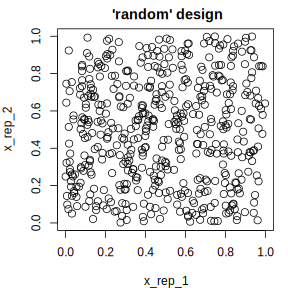
\includegraphics[width=0.45\linewidth]{mlr3book_files/figure-latex/05-technical-049-1} 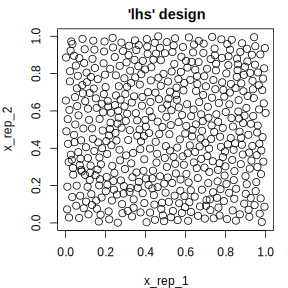
\includegraphics[width=0.45\linewidth]{mlr3book_files/figure-latex/05-technical-049-2} \end{center}

\hypertarget{generalized-sampling-the-sampler-class}{%
\subsubsection{\texorpdfstring{Generalized Sampling: The \texttt{Sampler} Class}{Generalized Sampling: The Sampler Class}}\label{generalized-sampling-the-sampler-class}}

It may sometimes be desirable to configure parameter sampling in more detail.
\href{https://paradox.mlr-org.com}{paradox} uses the \texttt{Sampler} abstract base class for sampling, which has many different sub-classes that can be parameterized and combined to control the sampling process.
It is even possible to create further sub-classes of the \texttt{Sampler} class (or of any of \emph{its} subclasses) for even more possibilities.

Every \texttt{Sampler} object has a \texttt{sample()} function, which takes one argument, the number of instances to sample, and returns a \protect\hyperlink{parameter-designs}{\texttt{Design}} object.

\hypertarget{d-samplers}{%
\paragraph{1D-Samplers}\label{d-samplers}}

There is a variety of samplers that sample values for a single parameter.
These are \texttt{Sampler1DUnif} (uniform sampling), \texttt{Sampler1DCateg} (sampling for categorical parameters), \texttt{Sampler1DNormal} (normally distributed sampling, truncated at parameter bounds), and \texttt{Sampler1DRfun} (arbitrary 1D sampling, given a random-function).
These are initialized with a single \texttt{Param}, and can then be used to sample values.

\begin{Shaded}
\begin{Highlighting}[]
\NormalTok{sampA =}\StringTok{ }\NormalTok{Sampler1DCateg}\OperatorTok{$}\KeywordTok{new}\NormalTok{(parA)}
\NormalTok{sampA}\OperatorTok{$}\KeywordTok{sample}\NormalTok{(}\DecValTok{5}\NormalTok{)}
\NormalTok{## <Design> with 5 rows:}
\NormalTok{##        A}
\NormalTok{## 1:  TRUE}
\NormalTok{## 2: FALSE}
\NormalTok{## 3:  TRUE}
\NormalTok{## 4: FALSE}
\NormalTok{## 5:  TRUE}
\end{Highlighting}
\end{Shaded}

\hypertarget{hierarchical-sampler}{%
\paragraph{Hierarchical Sampler}\label{hierarchical-sampler}}

The \texttt{SamplerHierarchical} sampler is an auxiliary sampler that combines many 1D-Samplers to get a combined distribution.
Its name ``hierarchical'' implies that it is able to respect parameter dependencies.
This suggests that parameters only get sampled when their dependencies are met.

The following example shows how this works: The \texttt{Int} parameter \texttt{B} depends on the \texttt{Lgl} parameter \texttt{A} being \texttt{TRUE}.
\texttt{A} is sampled to be \texttt{TRUE} in about half the cases, in which case \texttt{B} takes a value between 0 and 10.
In the cases where \texttt{A} is \texttt{FALSE}, \texttt{B} is set to \texttt{NA}.

\begin{Shaded}
\begin{Highlighting}[]
\NormalTok{psSmall}\OperatorTok{$}\KeywordTok{add_dep}\NormalTok{(}\StringTok{"B"}\NormalTok{, }\StringTok{"A"}\NormalTok{, CondEqual}\OperatorTok{$}\KeywordTok{new}\NormalTok{(}\OtherTok{TRUE}\NormalTok{))}
\NormalTok{sampH =}\StringTok{ }\NormalTok{SamplerHierarchical}\OperatorTok{$}\KeywordTok{new}\NormalTok{(psSmall, }\KeywordTok{list}\NormalTok{(Sampler1DCateg}\OperatorTok{$}\KeywordTok{new}\NormalTok{(parA), }
\NormalTok{  Sampler1DUnif}\OperatorTok{$}\KeywordTok{new}\NormalTok{(parB), Sampler1DUnif}\OperatorTok{$}\KeywordTok{new}\NormalTok{(parC)))}
\NormalTok{sampled =}\StringTok{ }\NormalTok{sampH}\OperatorTok{$}\KeywordTok{sample}\NormalTok{(}\DecValTok{1000}\NormalTok{)}
\KeywordTok{table}\NormalTok{(sampled}\OperatorTok{$}\NormalTok{data[, }\KeywordTok{c}\NormalTok{(}\StringTok{"A"}\NormalTok{, }\StringTok{"B"}\NormalTok{)], }\DataTypeTok{useNA =} \StringTok{"ifany"}\NormalTok{)}
\NormalTok{##        B}
\NormalTok{## A         0   1   2   3   4   5   6   7   8   9  10}
\NormalTok{##   FALSE   0   0   0   0   0   0   0   0   0   0   0}
\NormalTok{##   TRUE   55  54  41  49  38  54  35  42  47  46  43}
\NormalTok{##        B}
\NormalTok{## A       <NA>}
\NormalTok{##   FALSE  496}
\NormalTok{##   TRUE     0}
\end{Highlighting}
\end{Shaded}

\hypertarget{joint-sampler}{%
\paragraph{Joint Sampler}\label{joint-sampler}}

Another way of combining samplers is the \texttt{SamplerJointIndep}.
\texttt{SamplerJointIndep} also makes it possible to combine \texttt{Sampler}s that are not 1D.
However, \texttt{SamplerJointIndep} currently can not handle \texttt{ParamSet}s with dependencies.

\begin{Shaded}
\begin{Highlighting}[]
\NormalTok{sampJ =}\StringTok{ }\NormalTok{SamplerJointIndep}\OperatorTok{$}\KeywordTok{new}\NormalTok{(}\KeywordTok{list}\NormalTok{(Sampler1DUnif}\OperatorTok{$}\KeywordTok{new}\NormalTok{(ParamDbl}\OperatorTok{$}\KeywordTok{new}\NormalTok{(}\StringTok{"x"}\NormalTok{, }
  \DecValTok{0}\NormalTok{, }\DecValTok{1}\NormalTok{)), Sampler1DUnif}\OperatorTok{$}\KeywordTok{new}\NormalTok{(ParamDbl}\OperatorTok{$}\KeywordTok{new}\NormalTok{(}\StringTok{"y"}\NormalTok{, }\DecValTok{0}\NormalTok{, }\DecValTok{1}\NormalTok{))))}
\NormalTok{sampJ}\OperatorTok{$}\KeywordTok{sample}\NormalTok{(}\DecValTok{5}\NormalTok{)}
\NormalTok{## <Design> with 5 rows:}
\NormalTok{##         x      y}
\NormalTok{## 1: 0.7068 0.7112}
\NormalTok{## 2: 0.9676 0.1795}
\NormalTok{## 3: 0.2373 0.5154}
\NormalTok{## 4: 0.9031 0.2450}
\NormalTok{## 5: 0.8957 0.7116}
\end{Highlighting}
\end{Shaded}

\hypertarget{samplerunif}{%
\paragraph{SamplerUnif}\label{samplerunif}}

The \texttt{Sampler} used in \texttt{generate\_design\_random} is the \texttt{SamplerUnif} sampler, which corresponds to a \texttt{HierarchicalSampler} of \texttt{Sampler1DUnif} for all parameters.

\hypertarget{parameter-transformation}{%
\subsection{Parameter Transformation}\label{parameter-transformation}}

While the different \texttt{Sampler}s allow for a wide specification of parameter distributions, there are cases where the simplest way of getting a desired distribution is to sample parameters from a simple distribution (such as the uniform distribution) and then transform them.
This can be done by assigning a function to the \texttt{\$trafo} slot of a \texttt{ParamSet}.
The \texttt{\$trafo} function is called with two parameters:

\begin{itemize}
\tightlist
\item
  The list of parameter values to be transformed as \texttt{x}
\item
  The \texttt{ParamSet} itself as \texttt{param\_set}
\end{itemize}

The \texttt{\$trafo} function must return a list of transformed parameter values.

The transformation is performed when calling the \texttt{\$transpose} function of the \texttt{Design} object returned by a \texttt{Sampler} with the \texttt{trafo} ParamSet to \texttt{TRUE} (the default).
The following, for example, creates a parameter that is exponentially distributed:

\begin{Shaded}
\begin{Highlighting}[]
\NormalTok{psexp =}\StringTok{ }\NormalTok{ParamSet}\OperatorTok{$}\KeywordTok{new}\NormalTok{(}\KeywordTok{list}\NormalTok{(ParamDbl}\OperatorTok{$}\KeywordTok{new}\NormalTok{(}\StringTok{"par"}\NormalTok{, }\DecValTok{0}\NormalTok{, }\DecValTok{1}\NormalTok{)))}
\NormalTok{psexp}\OperatorTok{$}\NormalTok{trafo =}\StringTok{ }\ControlFlowTok{function}\NormalTok{(x, param_set) \{}
\NormalTok{  x}\OperatorTok{$}\NormalTok{par =}\StringTok{ }\OperatorTok{-}\KeywordTok{log}\NormalTok{(x}\OperatorTok{$}\NormalTok{par)}
\NormalTok{  x}
\NormalTok{\}}
\NormalTok{design =}\StringTok{ }\KeywordTok{generate_design_random}\NormalTok{(psexp, }\DecValTok{2}\NormalTok{)}
\KeywordTok{print}\NormalTok{(design)}
\NormalTok{## <Design> with 2 rows:}
\NormalTok{##       par}
\NormalTok{## 1: 0.5500}
\NormalTok{## 2: 0.5163}
\NormalTok{design}\OperatorTok{$}\KeywordTok{transpose}\NormalTok{()  }\CommentTok{# trafo is TRUE}
\NormalTok{## [[1]]}
\NormalTok{## [[1]]$par}
\NormalTok{## [1] 0.5978}
\NormalTok{## }
\NormalTok{## }
\NormalTok{## [[2]]}
\NormalTok{## [[2]]$par}
\NormalTok{## [1] 0.6611}
\end{Highlighting}
\end{Shaded}

Compare this to \texttt{\$transpose()} without transformation:

\begin{Shaded}
\begin{Highlighting}[]
\NormalTok{design}\OperatorTok{$}\KeywordTok{transpose}\NormalTok{(}\DataTypeTok{trafo =} \OtherTok{FALSE}\NormalTok{)}
\NormalTok{## [[1]]}
\NormalTok{## [[1]]$par}
\NormalTok{## [1] 0.55}
\NormalTok{## }
\NormalTok{## }
\NormalTok{## [[2]]}
\NormalTok{## [[2]]$par}
\NormalTok{## [1] 0.5163}
\end{Highlighting}
\end{Shaded}

\hypertarget{transformation-between-types}{%
\subsubsection{Transformation between Types}\label{transformation-between-types}}

Usually the design created with one \texttt{ParamSet} is then used to configure other objects that themselves have a \texttt{ParamSet} which defines the values they take.
The \texttt{ParamSet}s which can be used for random sampling, however, are restricted in some ways:
They must have finite bounds, and they may not contain ``untyped'' (\texttt{ParamUty}) parameters.
\texttt{\$trafo} provides the glue for these situations.
There is relatively little constraint on the trafo function's return value, so it is possible to return values that have different bounds or even types than the original \texttt{ParamSet}.
It is even possible to remove some parameters and add new ones.

Suppose, for example, that a certain method requires a \emph{function} as a parameter.
Let's say a function that summarizes its data in a certain way.
The user can pass functions like \texttt{median()} or \texttt{mean()}, but could also pass quantiles or something completely different.
This method would probably use the following \texttt{ParamSet}:

\begin{Shaded}
\begin{Highlighting}[]
\NormalTok{methodPS =}\StringTok{ }\NormalTok{ParamSet}\OperatorTok{$}\KeywordTok{new}\NormalTok{(}\KeywordTok{list}\NormalTok{(ParamUty}\OperatorTok{$}\KeywordTok{new}\NormalTok{(}\StringTok{"fun"}\NormalTok{, }\DataTypeTok{custom_check =} \ControlFlowTok{function}\NormalTok{(x) checkmate}\OperatorTok{::}\KeywordTok{checkFunction}\NormalTok{(x, }
  \DataTypeTok{nargs =} \DecValTok{1}\NormalTok{))))}
\KeywordTok{print}\NormalTok{(methodPS)}
\NormalTok{## ParamSet: }
\NormalTok{##     id    class lower upper levels     default value}
\NormalTok{## 1: fun ParamUty    NA    NA        <NoDefault>}
\end{Highlighting}
\end{Shaded}

If one wanted to sample this method, using one of four functions, a way to do this would be:

\begin{Shaded}
\begin{Highlighting}[]
\NormalTok{samplingPS =}\StringTok{ }\NormalTok{ParamSet}\OperatorTok{$}\KeywordTok{new}\NormalTok{(}\KeywordTok{list}\NormalTok{(ParamFct}\OperatorTok{$}\KeywordTok{new}\NormalTok{(}\StringTok{"fun"}\NormalTok{, }\KeywordTok{c}\NormalTok{(}\StringTok{"mean"}\NormalTok{, }
  \StringTok{"median"}\NormalTok{, }\StringTok{"min"}\NormalTok{, }\StringTok{"max"}\NormalTok{))))}

\NormalTok{samplingPS}\OperatorTok{$}\NormalTok{trafo =}\StringTok{ }\ControlFlowTok{function}\NormalTok{(x, param_set) \{}
  \CommentTok{# x$fun is a `character(1)`, in particular one of 'mean',}
  \CommentTok{# 'median', 'min', 'max'.  We want to turn it into a}
  \CommentTok{# function!}
\NormalTok{  x}\OperatorTok{$}\NormalTok{fun =}\StringTok{ }\KeywordTok{get}\NormalTok{(x}\OperatorTok{$}\NormalTok{fun, }\DataTypeTok{mode =} \StringTok{"function"}\NormalTok{)}
\NormalTok{  x}
\NormalTok{\}}
\end{Highlighting}
\end{Shaded}

\begin{Shaded}
\begin{Highlighting}[]
\NormalTok{design =}\StringTok{ }\KeywordTok{generate_design_random}\NormalTok{(samplingPS, }\DecValTok{2}\NormalTok{)}
\KeywordTok{print}\NormalTok{(design)}
\NormalTok{## <Design> with 2 rows:}
\NormalTok{##    fun}
\NormalTok{## 1: min}
\NormalTok{## 2: min}
\end{Highlighting}
\end{Shaded}

Note that the \texttt{Design} only contains the column ``\texttt{fun}'' as a \texttt{character} column.
To get a single value as a \emph{function}, the \texttt{\$transpose} function is used.

\begin{Shaded}
\begin{Highlighting}[]
\NormalTok{xvals =}\StringTok{ }\NormalTok{design}\OperatorTok{$}\KeywordTok{transpose}\NormalTok{()}
\KeywordTok{print}\NormalTok{(xvals[[}\DecValTok{1}\NormalTok{]])}
\NormalTok{## $fun}
\NormalTok{## function (..., na.rm = FALSE)  .Primitive("min")}
\end{Highlighting}
\end{Shaded}

We can now check that it fits the requirements set by \texttt{methodPS}, and that \texttt{fun} it is in fact a function:

\begin{Shaded}
\begin{Highlighting}[]
\NormalTok{methodPS}\OperatorTok{$}\KeywordTok{check}\NormalTok{(xvals[[}\DecValTok{1}\NormalTok{]])}
\NormalTok{## [1] TRUE}
\NormalTok{xvals[[}\DecValTok{1}\NormalTok{]]}\OperatorTok{$}\KeywordTok{fun}\NormalTok{(}\DecValTok{1}\OperatorTok{:}\DecValTok{10}\NormalTok{)}
\NormalTok{## [1] 1}
\end{Highlighting}
\end{Shaded}

Imagine now that a different kind of parametrization of the function is desired:
The user wants to give a function that selects a certain quantile, where the quantile is set by a parameter.
In that case the \texttt{\$transpose} function could generate a function in a different way.
For interpretability, the parameter is called ``\texttt{quantile}'' before transformation, and the ``\texttt{fun}'' parameter is generated on the fly.

\begin{Shaded}
\begin{Highlighting}[]
\NormalTok{samplingPS2 =}\StringTok{ }\NormalTok{ParamSet}\OperatorTok{$}\KeywordTok{new}\NormalTok{(}\KeywordTok{list}\NormalTok{(ParamDbl}\OperatorTok{$}\KeywordTok{new}\NormalTok{(}\StringTok{"quantile"}\NormalTok{, }
  \DecValTok{0}\NormalTok{, }\DecValTok{1}\NormalTok{)))}

\NormalTok{samplingPS2}\OperatorTok{$}\NormalTok{trafo =}\StringTok{ }\ControlFlowTok{function}\NormalTok{(x, param_set) \{}
  \CommentTok{# x$quantile is a `numeric(1)` between 0 and 1.  We want}
  \CommentTok{# to turn it into a function!}
  \KeywordTok{list}\NormalTok{(}\DataTypeTok{fun =} \ControlFlowTok{function}\NormalTok{(input) }\KeywordTok{quantile}\NormalTok{(input, x}\OperatorTok{$}\NormalTok{quantile))}
\NormalTok{\}}
\end{Highlighting}
\end{Shaded}

\begin{Shaded}
\begin{Highlighting}[]
\NormalTok{design =}\StringTok{ }\KeywordTok{generate_design_random}\NormalTok{(samplingPS2, }\DecValTok{2}\NormalTok{)}
\KeywordTok{print}\NormalTok{(design)}
\NormalTok{## <Design> with 2 rows:}
\NormalTok{##    quantile}
\NormalTok{## 1: 0.004436}
\NormalTok{## 2: 0.660597}
\end{Highlighting}
\end{Shaded}

The \texttt{Design} now contains the column ``\texttt{quantile}'' that will be used by the \texttt{\$transpose} function to create the \texttt{fun} parameter.
We also check that it fits the requirement set by \texttt{methodPS}, and that it is a function.

\begin{Shaded}
\begin{Highlighting}[]
\NormalTok{xvals =}\StringTok{ }\NormalTok{design}\OperatorTok{$}\KeywordTok{transpose}\NormalTok{()}
\KeywordTok{print}\NormalTok{(xvals[[}\DecValTok{1}\NormalTok{]])}
\NormalTok{## $fun}
\NormalTok{## function(input) quantile(input, x$quantile)}
\NormalTok{## <environment: 0x12912160>}
\NormalTok{methodPS}\OperatorTok{$}\KeywordTok{check}\NormalTok{(xvals[[}\DecValTok{1}\NormalTok{]])}
\NormalTok{## [1] TRUE}
\NormalTok{xvals[[}\DecValTok{1}\NormalTok{]]}\OperatorTok{$}\KeywordTok{fun}\NormalTok{(}\DecValTok{1}\OperatorTok{:}\DecValTok{10}\NormalTok{)}
\NormalTok{## 0.4436% }
\NormalTok{##    1.04}
\end{Highlighting}
\end{Shaded}

\hypertarget{logging}{%
\section{Logging and Verbosity}\label{logging}}

We use the \texttt{lgr} package for logging and progress output.

Because \emph{lgr} comes with its own exhaustive vignette, we will just briefly give examples how you can change the most important settings related to logging in \href{https://mlr3.mlr-org.com}{mlr3}.

\hypertarget{available-logging-levels}{%
\subsection{Available logging levels}\label{available-logging-levels}}

\emph{lgr} comes with certain numeric thresholds which correspond to verbosity levels of the logging.
For \href{https://mlr3.mlr-org.com}{mlr3} the default is set to 400 which corresponds to level ``info''.
The following ones are available:

\begin{Shaded}
\begin{Highlighting}[]
\KeywordTok{library}\NormalTok{(}\StringTok{"lgr"}\NormalTok{)}
\KeywordTok{getOption}\NormalTok{(}\StringTok{"lgr.log_levels"}\NormalTok{)}
\NormalTok{## fatal error  warn  info debug trace }
\NormalTok{##   100   200   300   400   500   600}
\end{Highlighting}
\end{Shaded}

\hypertarget{global-setting}{%
\subsection{Global Setting}\label{global-setting}}

\emph{lgr} comes with a global option called \texttt{"lgr.default\_threshold"} which can be set via \texttt{options()}.
You can set a specific level in your \texttt{.Rprofile} which is then used for all packages that use the \emph{lgr} package.
This approach may not be desirable if you want to only change the logging level for \href{https://mlr3.mlr-org.com}{mlr3}.

\hypertarget{changing-mlr3-logging-levels}{%
\subsection{Changing mlr3 logging levels}\label{changing-mlr3-logging-levels}}

To change the setting for \href{https://mlr3.mlr-org.com}{mlr3} only, you need to change the threshold of the \href{https://mlr3.mlr-org.com}{mlr3} logger like this:

\begin{Shaded}
\begin{Highlighting}[]
\NormalTok{lgr}\OperatorTok{::}\KeywordTok{get_logger}\NormalTok{(}\StringTok{"mlr3"}\NormalTok{)}\OperatorTok{$}\KeywordTok{set_threshold}\NormalTok{(}\StringTok{"<level>"}\NormalTok{)}
\end{Highlighting}
\end{Shaded}

Remember that this change only applies to the current R session.

\hypertarget{transition}{%
\section{mlr -\textgreater{} mlr3 Transition Guide}\label{transition}}

In case you have already worked with \texttt{mlr}, you may want to quickstart with \href{https://mlr3.mlr-org.com}{mlr3} by looking up the specific equivalent of an element of \texttt{mlr} in the new version \href{https://mlr3.mlr-org.com}{mlr3}.
For this, you can use the following table.
This table is not complete but should give you an overview about how \href{https://mlr3.mlr-org.com}{mlr3} is organized.

\includegraphics[width=7.00in,height=5.96in,keepaspectratio]{mlr3book_files/figure-latex/05-technical-065-1.png}

\includegraphics[width=7.00in,height=6.86in,keepaspectratio]{mlr3book_files/figure-latex/05-technical-066-1.png}

\includegraphics[width=7.00in,height=7.90in,keepaspectratio]{mlr3book_files/figure-latex/05-technical-067-1.png}

\includegraphics[width=7.00in,height=7.28in,keepaspectratio]{mlr3book_files/figure-latex/05-technical-068-1.png}

\includegraphics[width=7.00in,height=10.44in,keepaspectratio]{mlr3book_files/figure-latex/05-technical-069-1.png}

\includegraphics[width=7.00in,height=8.12in,keepaspectratio]{mlr3book_files/figure-latex/05-technical-070-1.png}

\includegraphics[width=7.00in,height=6.80in,keepaspectratio]{mlr3book_files/figure-latex/05-technical-071-1.png}

\hypertarget{extending}{%
\chapter{Extending}\label{extending}}

This chapter gives instructions on how to extend \href{https://mlr3.mlr-org.com}{mlr3} and its extension packages with custom objects.

The approach is always the same:

\begin{enumerate}
\def\labelenumi{\arabic{enumi}.}
\tightlist
\item
  determine the base class you want to inherit from,
\item
  extend the class with your custom functionality,
\item
  test your implementation
\item
  (optionally) add new object to the respective \texttt{Dictionary}.
\end{enumerate}

The chapter \protect\hyperlink{ext-learner}{Create a new learner} illustrates the steps needed to create a custom learner in mlr3.

\hypertarget{ext-learner}{%
\section{Extending with Learners}\label{ext-learner}}

Here, we show how to create a custom \texttt{LearnerClassif} step-by-step.

Preferably, you checkout our \href{https://github.com/mlr-org/mlr3learnertemplate}{template package} for new learners.
Alternatively, here is a template snippet for a new classification learner:

\begin{Shaded}
\begin{Highlighting}[]
\NormalTok{LearnerClassifYourLearner =}\StringTok{ }\NormalTok{R6}\OperatorTok{::}\KeywordTok{R6Class}\NormalTok{(}\StringTok{"LearnerClassifYourLearner"}\NormalTok{,}
  \DataTypeTok{inherit =}\NormalTok{ LearnerClassif,}
  \DataTypeTok{public =} \KeywordTok{list}\NormalTok{(}
    \DataTypeTok{initialize =} \ControlFlowTok{function}\NormalTok{(}\DataTypeTok{id =} \StringTok{"classif.yourlearner"}\NormalTok{) \{}
\NormalTok{      super}\OperatorTok{$}\KeywordTok{initialize}\NormalTok{(}
        \DataTypeTok{id =}\NormalTok{ id,}
        \DataTypeTok{param_set =}\NormalTok{ ParamSet}\OperatorTok{$}\KeywordTok{new}\NormalTok{(),}
        \DataTypeTok{predict_types =}\NormalTok{ ,}
        \DataTypeTok{feature_types =}\NormalTok{ ,}
        \DataTypeTok{properties =}\NormalTok{ ,}
        \DataTypeTok{packages =}\NormalTok{ ,}
\NormalTok{      )}
\NormalTok{    \},}

    \DataTypeTok{train =} \ControlFlowTok{function}\NormalTok{(task) \{}

\NormalTok{    \},}
    \DataTypeTok{predict =} \ControlFlowTok{function}\NormalTok{(task) \{}

\NormalTok{    \}}
\NormalTok{  )}
\NormalTok{)}
\end{Highlighting}
\end{Shaded}

In the first line of the template, we create a new \texttt{R6} class with class \texttt{"LearnerClassifYourLearner"}.
The next line determines the parent class:
As we want to create a classification learner, we obviously want to inherit from \texttt{LearnerClassif}.

A learner consists of three parts:

\begin{enumerate}
\def\labelenumi{\arabic{enumi}.}
\tightlist
\item
  \protect\hyperlink{learner-meta-information}{Meta information} about the learners
\item
  A \protect\hyperlink{learner-train}{\texttt{train\_internal()} function} which takes a (filtered) \texttt{TaskClassif} and returns a model
\item
  A \protect\hyperlink{learner-predict}{\texttt{predict\_internal()} function} which operates on the model in \texttt{self\$model} (stored during \texttt{\$train()}) and a (differently subsetted) \texttt{TaskClassif} to return a named list of predictions.
\end{enumerate}

\hypertarget{learner-meta-information}{%
\subsection{Meta-information}\label{learner-meta-information}}

In the constructor function \texttt{initialize()} the constructor of the super class \texttt{LearnerClassif} is called with meta information about the learner we want to construct.
This includes:

\begin{itemize}
\tightlist
\item
  \texttt{id}: The id of the new learner.
\item
  \texttt{packages}: Set of required packages to run the learner.
\item
  \texttt{param\_set}: A set of hyperparameters and their description, provided as \texttt{paradox::ParamSet}.
  It is perfectly fine to add no parameters here for a first draft.
  For each hyperparameter you want to add, you have to select the appropriate class:

  \begin{itemize}
  \tightlist
  \item
    \texttt{paradox::ParamLgl} for scalar logical hyperparameters.
  \item
    \texttt{paradox::ParamInt} for scalar integer hyperparameters.
  \item
    \texttt{paradox::ParamDbl} for scalar numeric hyperparameters.
  \item
    \texttt{paradox::ParamFct} for scalar factor hyperparameters (this includes characters).
  \item
    \texttt{paradox::ParamUty} for everything else.
  \end{itemize}
\item
  \texttt{predict\_types}: Set of predict types the learner is capable of.
  These differ depending on the type of the learner.

  \begin{itemize}
  \tightlist
  \item
    \texttt{LearnerClassif}

    \begin{itemize}
    \tightlist
    \item
      \texttt{response}: Only predicts a class label for each observation in the test set.
    \item
      \texttt{prob}: Also predicts the posterior probability for each class for each observation in the test set.
    \end{itemize}
  \item
    \texttt{LearnerRegr}

    \begin{itemize}
    \tightlist
    \item
      \texttt{response}: Only predicts a numeric response for each observation in the test set.
    \item
      \texttt{se}: Also predicts the standard error for each value of response for each observation in the test set.
    \end{itemize}
  \end{itemize}
\item
  \texttt{feature\_types}: Set of feature types the learner can handle.
  See \texttt{mlr\_reflections",\ text\ =\ "mlr\_reflections\$task\_feature\_types} for feature types supported by \href{https://mlr3.mlr-org.com}{mlr3}.
\item
  \texttt{properties}: Set of properties of the learner. Possible properties include:

  \begin{itemize}
  \tightlist
  \item
    \texttt{"twoclass"}: The learner works on binary classification problems.
  \item
    \texttt{"multiclass"}: The learner works on multi-class classification problems.
  \item
    \texttt{"missings"}: The learner can natively handle missing values.
  \item
    \texttt{"weights"}: The learner can work on tasks which have observation weights / case weights.
  \item
    \texttt{"parallel"}: The learner can be parallelized, e.g.~via threading.
  \item
    \texttt{"importance"}: The learner supports extracting importance values for features.
    If this property is set, you must also implement a public method \texttt{importance()} to retrieve the importance values from the model.
  \item
    \texttt{"selected\_features"}: The learner supports extracting the features which where used.
    If this property is set, you must also implement a public method \texttt{selected\_features()} to retrieve the set of used features from the model.
  \end{itemize}
\end{itemize}

For a simplified \texttt{rpart::rpart()}, the initialization could look like this:

\begin{Shaded}
\begin{Highlighting}[]
\NormalTok{initialize =}\StringTok{ }\ControlFlowTok{function}\NormalTok{(}\DataTypeTok{id =} \StringTok{"classif.rpart"}\NormalTok{) \{}
\NormalTok{  ps =}\StringTok{ }\NormalTok{ParamSet}\OperatorTok{$}\KeywordTok{new}\NormalTok{(}\KeywordTok{list}\NormalTok{(ParamDbl}\OperatorTok{$}\KeywordTok{new}\NormalTok{(}\DataTypeTok{id =} \StringTok{"cp"}\NormalTok{, }\DataTypeTok{default =} \FloatTok{0.01}\NormalTok{, }
    \DataTypeTok{lower =} \DecValTok{0}\NormalTok{, }\DataTypeTok{upper =} \DecValTok{1}\NormalTok{, }\DataTypeTok{tags =} \StringTok{"train"}\NormalTok{), ParamInt}\OperatorTok{$}\KeywordTok{new}\NormalTok{(}\DataTypeTok{id =} \StringTok{"xval"}\NormalTok{, }
    \DataTypeTok{default =}\NormalTok{ 10L, }\DataTypeTok{lower =}\NormalTok{ 0L, }\DataTypeTok{tags =} \StringTok{"train"}\NormalTok{)))}
\NormalTok{  ps}\OperatorTok{$}\NormalTok{values =}\StringTok{ }\KeywordTok{list}\NormalTok{(}\DataTypeTok{xval =}\NormalTok{ 0L)}
  
\NormalTok{  super}\OperatorTok{$}\KeywordTok{initialize}\NormalTok{(}\DataTypeTok{id =}\NormalTok{ id, }\DataTypeTok{packages =} \StringTok{"rpart"}\NormalTok{, }\DataTypeTok{feature_types =} \KeywordTok{c}\NormalTok{(}\StringTok{"logical"}\NormalTok{, }
    \StringTok{"integer"}\NormalTok{, }\StringTok{"numeric"}\NormalTok{, }\StringTok{"factor"}\NormalTok{), }\DataTypeTok{predict_types =} \KeywordTok{c}\NormalTok{(}\StringTok{"response"}\NormalTok{, }
    \StringTok{"prob"}\NormalTok{), }\DataTypeTok{param_set =}\NormalTok{ ps, }\DataTypeTok{properties =} \KeywordTok{c}\NormalTok{(}\StringTok{"twoclass"}\NormalTok{, }
    \StringTok{"multiclass"}\NormalTok{, }\StringTok{"weights"}\NormalTok{, }\StringTok{"missings"}\NormalTok{))}
\NormalTok{\}}
\end{Highlighting}
\end{Shaded}

We only have specified a small subset of the available hyperparameters:

\begin{itemize}
\tightlist
\item
  The complexity \texttt{"cp"} is numeric, its feasible range is \texttt{{[}0,1{]}}, it defaults to \texttt{0.01} and the parameter is used during \texttt{"train"}.
\item
  The complexity \texttt{"xval"} is integer, its lower bound \texttt{0}, its default is \texttt{0} and the parameter is also used during \texttt{"train"}.
  Note that we have changed the default here from \texttt{10} to \texttt{0} to save some computation time.
  This is \textbf{not} done by setting a different \texttt{default} in \texttt{ParamInt\$new()}, but instead by setting the value explicitly.
\end{itemize}

\hypertarget{learner-train}{%
\subsection{Train function}\label{learner-train}}

We continue the to adept the template for a \texttt{rpart::rpart()} learner, and now tackle the \texttt{train\_internal()} function.
The train function takes a \texttt{Task} as input and must return an arbitrary model.
First, we write something down that works completely without \href{https://mlr3.mlr-org.com}{mlr3}:

\begin{Shaded}
\begin{Highlighting}[]
\NormalTok{data =}\StringTok{ }\NormalTok{iris}
\NormalTok{model =}\StringTok{ }\NormalTok{rpart}\OperatorTok{::}\KeywordTok{rpart}\NormalTok{(Species }\OperatorTok{~}\StringTok{ }\NormalTok{., }\DataTypeTok{data =}\NormalTok{ iris, }\DataTypeTok{xval =} \DecValTok{0}\NormalTok{)}
\end{Highlighting}
\end{Shaded}

In the next step, we replace the data frame \texttt{data} with a \texttt{Task}:

\begin{Shaded}
\begin{Highlighting}[]
\NormalTok{task =}\StringTok{ }\KeywordTok{tsk}\NormalTok{(}\StringTok{"iris"}\NormalTok{)}
\NormalTok{model =}\StringTok{ }\NormalTok{rpart}\OperatorTok{::}\KeywordTok{rpart}\NormalTok{(Species }\OperatorTok{~}\StringTok{ }\NormalTok{., }\DataTypeTok{data =}\NormalTok{ task}\OperatorTok{$}\KeywordTok{data}\NormalTok{(), }\DataTypeTok{xval =} \DecValTok{0}\NormalTok{)}
\end{Highlighting}
\end{Shaded}

The target variable \texttt{"Species"} is still hard-coded and specific to the task.
This is unnecessary, as the information about the target variable is stored in the task:

\begin{Shaded}
\begin{Highlighting}[]
\NormalTok{task}\OperatorTok{$}\NormalTok{target_names}
\NormalTok{## [1] "Species"}
\NormalTok{task}\OperatorTok{$}\KeywordTok{formula}\NormalTok{()}
\NormalTok{## Species ~ .}
\NormalTok{## NULL}
\end{Highlighting}
\end{Shaded}

We can adapt our code accordingly:

\begin{Shaded}
\begin{Highlighting}[]
\NormalTok{rpart}\OperatorTok{::}\KeywordTok{rpart}\NormalTok{(task}\OperatorTok{$}\KeywordTok{formula}\NormalTok{(), }\DataTypeTok{data =}\NormalTok{ task}\OperatorTok{$}\KeywordTok{data}\NormalTok{(), }\DataTypeTok{xval =} \DecValTok{0}\NormalTok{)}
\NormalTok{## n= 150 }
\NormalTok{## }
\NormalTok{## node), split, n, loss, yval, (yprob)}
\NormalTok{##       * denotes terminal node}
\NormalTok{## }
\NormalTok{## 1) root 150 100 setosa (0.33333 0.33333 0.33333)  }
\NormalTok{##   2) Petal.Length< 2.45 50   0 setosa (1.00000 0.00000 0.00000) *}
\NormalTok{##   3) Petal.Length>=2.45 100  50 versicolor (0.00000 0.50000 0.50000)  }
\NormalTok{##     6) Petal.Width< 1.75 54   5 versicolor (0.00000 0.90741 0.09259) *}
\NormalTok{##     7) Petal.Width>=1.75 46   1 virginica (0.00000 0.02174 0.97826) *}
\end{Highlighting}
\end{Shaded}

The last thing missing is the handling of hyperparameters.
Instead of the hard-coded \texttt{xval}, we query the hyperparameter settings from the \texttt{Learner} itself.

To illustrate this, we quickly construct the tree learner from the \href{https://mlr3.mlr-org.com}{mlr3} package, and use the method \texttt{get\_value()} from the \texttt{ParamSet} to retrieve all set hyperparameters with tag \texttt{"train"}.

\begin{Shaded}
\begin{Highlighting}[]
\NormalTok{self =}\StringTok{ }\KeywordTok{lrn}\NormalTok{(}\StringTok{"classif.rpart"}\NormalTok{)}
\NormalTok{self}\OperatorTok{$}\NormalTok{param_set}\OperatorTok{$}\KeywordTok{get_values}\NormalTok{(}\DataTypeTok{tags =} \StringTok{"train"}\NormalTok{)}
\NormalTok{## $xval}
\NormalTok{## [1] 0}
\end{Highlighting}
\end{Shaded}

To pass all hyperparameters down to the model fitting function, we recommend to use either \texttt{do.call} or the function \texttt{mlr3misc::invoke()}.

\begin{Shaded}
\begin{Highlighting}[]
\NormalTok{pars =}\StringTok{ }\NormalTok{self}\OperatorTok{$}\NormalTok{param_set}\OperatorTok{$}\KeywordTok{get_values}\NormalTok{(}\DataTypeTok{tags =} \StringTok{"train"}\NormalTok{)}
\NormalTok{mlr3misc}\OperatorTok{::}\KeywordTok{invoke}\NormalTok{(rpart}\OperatorTok{::}\NormalTok{rpart, task}\OperatorTok{$}\KeywordTok{formula}\NormalTok{(), }\DataTypeTok{data =}\NormalTok{ task}\OperatorTok{$}\KeywordTok{data}\NormalTok{(), }
  \DataTypeTok{.args =}\NormalTok{ pars)}
\NormalTok{## n= 150 }
\NormalTok{## }
\NormalTok{## node), split, n, loss, yval, (yprob)}
\NormalTok{##       * denotes terminal node}
\NormalTok{## }
\NormalTok{## 1) root 150 100 setosa (0.33333 0.33333 0.33333)  }
\NormalTok{##   2) Petal.Length< 2.45 50   0 setosa (1.00000 0.00000 0.00000) *}
\NormalTok{##   3) Petal.Length>=2.45 100  50 versicolor (0.00000 0.50000 0.50000)  }
\NormalTok{##     6) Petal.Width< 1.75 54   5 versicolor (0.00000 0.90741 0.09259) *}
\NormalTok{##     7) Petal.Width>=1.75 46   1 virginica (0.00000 0.02174 0.97826) *}
\end{Highlighting}
\end{Shaded}

In the final learner, \texttt{self} will of course reference the learner itself.
In the last step, we wrap everything in a function.

\begin{Shaded}
\begin{Highlighting}[]
\NormalTok{train_internal =}\StringTok{ }\ControlFlowTok{function}\NormalTok{(task) \{}
\NormalTok{  pars =}\StringTok{ }\NormalTok{self}\OperatorTok{$}\NormalTok{param_set}\OperatorTok{$}\KeywordTok{get_values}\NormalTok{(}\DataTypeTok{tags =} \StringTok{"train"}\NormalTok{)}
\NormalTok{  mlr3misc}\OperatorTok{::}\KeywordTok{invoke}\NormalTok{(rpart}\OperatorTok{::}\NormalTok{rpart, task}\OperatorTok{$}\KeywordTok{formula}\NormalTok{(), }\DataTypeTok{data =}\NormalTok{ task}\OperatorTok{$}\KeywordTok{data}\NormalTok{(), }
    \DataTypeTok{.args =}\NormalTok{ pars)}
\NormalTok{\}}
\end{Highlighting}
\end{Shaded}

\hypertarget{learner-predict}{%
\subsection{Predict function}\label{learner-predict}}

The internal predict function \texttt{predict\_internal} also operates on a \texttt{Task} as well as on the model stored during \texttt{train()} in \texttt{self\$model}.
The return value is a \texttt{Prediction} object.
We proceed analogously to the section on the train function.
We start with a version without any \href{https://mlr3.mlr-org.com}{mlr3} objects and continue to replace objects until we have reached the desired interface:

\begin{Shaded}
\begin{Highlighting}[]
\CommentTok{# inputs:}
\NormalTok{task =}\StringTok{ }\KeywordTok{tsk}\NormalTok{(}\StringTok{"iris"}\NormalTok{)}
\NormalTok{self =}\StringTok{ }\KeywordTok{list}\NormalTok{(}\DataTypeTok{model =}\NormalTok{ rpart}\OperatorTok{::}\KeywordTok{rpart}\NormalTok{(task}\OperatorTok{$}\KeywordTok{formula}\NormalTok{(), }\DataTypeTok{data =}\NormalTok{ task}\OperatorTok{$}\KeywordTok{data}\NormalTok{()))}

\NormalTok{data =}\StringTok{ }\NormalTok{iris}
\NormalTok{response =}\StringTok{ }\KeywordTok{predict}\NormalTok{(self}\OperatorTok{$}\NormalTok{model, }\DataTypeTok{newdata =}\NormalTok{ data, }\DataTypeTok{type =} \StringTok{"class"}\NormalTok{)}
\NormalTok{prob =}\StringTok{ }\KeywordTok{predict}\NormalTok{(self}\OperatorTok{$}\NormalTok{model, }\DataTypeTok{newdata =}\NormalTok{ data, }\DataTypeTok{type =} \StringTok{"prob"}\NormalTok{)}
\end{Highlighting}
\end{Shaded}

The \texttt{rpart::predict.rpart()} function predicts class labels if argument \texttt{type} is set to to \texttt{"class"}, and class probabilities if set to \texttt{"prob"}.

Next, we transition from \texttt{data} to a \texttt{task} again and construct a proper \texttt{PredictionClassif} object to return.
Additionally, as we do not want to run the prediction twice, we differentiate what type of prediction is requested by querying the set predict type of the learner.
The complete \texttt{predict\_internal} function looks like this:

\begin{Shaded}
\begin{Highlighting}[]
\NormalTok{predict_internal =}\StringTok{ }\ControlFlowTok{function}\NormalTok{(task) \{}
\NormalTok{  self}\OperatorTok{$}\NormalTok{predict_type =}\StringTok{ "response"}
\NormalTok{  response =}\StringTok{ }\NormalTok{prob =}\StringTok{ }\OtherTok{NULL}
  
  \ControlFlowTok{if}\NormalTok{ (self}\OperatorTok{$}\NormalTok{predict_type }\OperatorTok{==}\StringTok{ "response"}\NormalTok{) \{}
\NormalTok{    response =}\StringTok{ }\KeywordTok{predict}\NormalTok{(self}\OperatorTok{$}\NormalTok{model, }\DataTypeTok{newdata =}\NormalTok{ task}\OperatorTok{$}\KeywordTok{data}\NormalTok{(), }
      \DataTypeTok{type =} \StringTok{"class"}\NormalTok{)}
\NormalTok{  \} }\ControlFlowTok{else}\NormalTok{ \{}
\NormalTok{    prob =}\StringTok{ }\KeywordTok{predict}\NormalTok{(self}\OperatorTok{$}\NormalTok{model, }\DataTypeTok{newdata =}\NormalTok{ task}\OperatorTok{$}\KeywordTok{data}\NormalTok{(), }
      \DataTypeTok{type =} \StringTok{"prob"}\NormalTok{)}
\NormalTok{  \}}
  
\NormalTok{  PredictionClassif}\OperatorTok{$}\KeywordTok{new}\NormalTok{(task, }\DataTypeTok{response =}\NormalTok{ response, }\DataTypeTok{prob =}\NormalTok{ prob)}
\NormalTok{\}}
\end{Highlighting}
\end{Shaded}

Note that if the learner would need to handle hyperparameters during the predict step, we would proceed analogously to the \texttt{train()} step and use \texttt{self\$params("predict} in combination with \texttt{mlr3misc::invoke()}.

Also note that you cannot rely on the column order of the data returned by \texttt{task\$data()}, i.e.~the order of columns may be different from the order of the columns during \texttt{\$train()}.
You have to make sure that your learner accesses columns by name, not by position (like some algorithms with a matrix interface do).
You may have to restore the order manually here, see \href{https://github.com/mlr-org/mlr3learners/blob/master/R/LearnerClassifSVM.R}{``classif.svm''} for an example.

\hypertarget{final-learner}{%
\subsection{Final learner}\label{final-learner}}

\begin{Shaded}
\begin{Highlighting}[]
\NormalTok{LearnerClassifYourRpart =}\StringTok{ }\NormalTok{R6}\OperatorTok{::}\KeywordTok{R6Class}\NormalTok{(}\StringTok{"LearnerClassifYourRpart"}\NormalTok{,}
  \DataTypeTok{inherit =}\NormalTok{ LearnerClassif,}
  \DataTypeTok{public =} \KeywordTok{list}\NormalTok{(}
    \DataTypeTok{initialize =} \ControlFlowTok{function}\NormalTok{(}\DataTypeTok{id =} \StringTok{"classif.rpart"}\NormalTok{) \{}
\NormalTok{      ps =}\StringTok{ }\NormalTok{ParamSet}\OperatorTok{$}\KeywordTok{new}\NormalTok{(}\KeywordTok{list}\NormalTok{(}
\NormalTok{        ParamDbl}\OperatorTok{$}\KeywordTok{new}\NormalTok{(}\DataTypeTok{id =} \StringTok{"cp"}\NormalTok{, }\DataTypeTok{default =} \FloatTok{0.01}\NormalTok{, }\DataTypeTok{lower =} \DecValTok{0}\NormalTok{, }\DataTypeTok{upper =} \DecValTok{1}\NormalTok{, }\DataTypeTok{tags =} \StringTok{"train"}\NormalTok{),}
\NormalTok{        ParamInt}\OperatorTok{$}\KeywordTok{new}\NormalTok{(}\DataTypeTok{id =} \StringTok{"xval"}\NormalTok{, }\DataTypeTok{default =}\NormalTok{ 0L, }\DataTypeTok{lower =}\NormalTok{ 0L, }\DataTypeTok{tags =} \StringTok{"train"}\NormalTok{)}
\NormalTok{      ))}
\NormalTok{      ps}\OperatorTok{$}\NormalTok{values =}\StringTok{ }\KeywordTok{list}\NormalTok{(}\DataTypeTok{xval =}\NormalTok{ 0L)}

\NormalTok{      super}\OperatorTok{$}\KeywordTok{initialize}\NormalTok{(}
        \DataTypeTok{id =}\NormalTok{ id,}
        \DataTypeTok{packages =} \StringTok{"rpart"}\NormalTok{,}
        \DataTypeTok{feature_types =} \KeywordTok{c}\NormalTok{(}\StringTok{"logical"}\NormalTok{, }\StringTok{"integer"}\NormalTok{, }\StringTok{"numeric"}\NormalTok{, }\StringTok{"factor"}\NormalTok{),}
        \DataTypeTok{predict_types =} \KeywordTok{c}\NormalTok{(}\StringTok{"response"}\NormalTok{, }\StringTok{"prob"}\NormalTok{),}
        \DataTypeTok{param_set =}\NormalTok{ ps,}
        \DataTypeTok{properties =} \KeywordTok{c}\NormalTok{(}\StringTok{"twoclass"}\NormalTok{, }\StringTok{"multiclass"}\NormalTok{, }\StringTok{"weights"}\NormalTok{, }\StringTok{"missings"}\NormalTok{)}
\NormalTok{      )}
\NormalTok{    \},}

    \DataTypeTok{train_internal =} \ControlFlowTok{function}\NormalTok{(task) \{}
\NormalTok{      pars =}\StringTok{ }\NormalTok{self}\OperatorTok{$}\NormalTok{param_set}\OperatorTok{$}\KeywordTok{get_values}\NormalTok{(}\DataTypeTok{tag =} \StringTok{"train"}\NormalTok{)}
\NormalTok{      mlr3misc}\OperatorTok{::}\KeywordTok{invoke}\NormalTok{(rpart}\OperatorTok{::}\NormalTok{rpart, task}\OperatorTok{$}\KeywordTok{formula}\NormalTok{(), }\DataTypeTok{data =}\NormalTok{ task}\OperatorTok{$}\KeywordTok{data}\NormalTok{(), }\DataTypeTok{.args =}\NormalTok{ pars)}
\NormalTok{    \},}

    \DataTypeTok{predict_internal =} \ControlFlowTok{function}\NormalTok{(task) \{}
\NormalTok{      self}\OperatorTok{$}\NormalTok{predict_type =}\StringTok{ "response"}
\NormalTok{      response =}\StringTok{ }\NormalTok{prob =}\StringTok{ }\OtherTok{NULL}

      \ControlFlowTok{if}\NormalTok{ (self}\OperatorTok{$}\NormalTok{predict_type }\OperatorTok{==}\StringTok{ "response"}\NormalTok{) \{}
\NormalTok{        response =}\StringTok{ }\KeywordTok{predict}\NormalTok{(self}\OperatorTok{$}\NormalTok{model, }\DataTypeTok{newdata =}\NormalTok{ task}\OperatorTok{$}\KeywordTok{data}\NormalTok{(), }\DataTypeTok{type =} \StringTok{"class"}\NormalTok{)}
\NormalTok{      \} }\ControlFlowTok{else}\NormalTok{ \{}
\NormalTok{        prob =}\StringTok{ }\KeywordTok{predict}\NormalTok{(self}\OperatorTok{$}\NormalTok{model, }\DataTypeTok{newdata =}\NormalTok{ task}\OperatorTok{$}\KeywordTok{data}\NormalTok{(), }\DataTypeTok{type =} \StringTok{"prob"}\NormalTok{)}
\NormalTok{      \}}
\NormalTok{      PredictionClassif}\OperatorTok{$}\KeywordTok{new}\NormalTok{(task, }\DataTypeTok{response =}\NormalTok{ response, }\DataTypeTok{prob =}\NormalTok{ prob)}
\NormalTok{    \}}
\NormalTok{  )}
\NormalTok{)}

\NormalTok{lrn =}\StringTok{ }\NormalTok{LearnerClassifYourRpart}\OperatorTok{$}\KeywordTok{new}\NormalTok{()}
\KeywordTok{print}\NormalTok{(lrn)}
\NormalTok{## <LearnerClassifYourRpart:classif.rpart>}
\NormalTok{## * Model: -}
\NormalTok{## * Parameters: xval=0}
\NormalTok{## * Packages: rpart}
\NormalTok{## * Predict Type: response}
\NormalTok{## * Feature types: logical, integer, numeric,}
\NormalTok{##   factor}
\NormalTok{## * Properties: missings, multiclass, twoclass,}
\NormalTok{##   weights}
\end{Highlighting}
\end{Shaded}

To run some basic tests:

\begin{Shaded}
\begin{Highlighting}[]
\NormalTok{task =}\StringTok{ }\KeywordTok{tsk}\NormalTok{(}\StringTok{"iris"}\NormalTok{)}
\NormalTok{lrn}\OperatorTok{$}\KeywordTok{train}\NormalTok{(task)}
\NormalTok{p =}\StringTok{ }\NormalTok{lrn}\OperatorTok{$}\KeywordTok{predict}\NormalTok{(task)}
\NormalTok{p}\OperatorTok{$}\NormalTok{confusion}
\NormalTok{##             truth}
\NormalTok{## response     setosa versicolor virginica}
\NormalTok{##   setosa         50          0         0}
\NormalTok{##   versicolor      0         49         5}
\NormalTok{##   virginica       0          1        45}
\end{Highlighting}
\end{Shaded}

To run a bunch of automatic tests, you may source some auxiliary scripts from the unit tests of \href{https://mlr3.mlr-org.com}{mlr3}:

\begin{Shaded}
\begin{Highlighting}[]
\NormalTok{helper =}\StringTok{ }\KeywordTok{list.files}\NormalTok{(}\KeywordTok{system.file}\NormalTok{(}\StringTok{"testthat"}\NormalTok{, }\DataTypeTok{package =} \StringTok{"mlr3"}\NormalTok{), }
  \DataTypeTok{pattern =} \StringTok{"^helper.*}\CharTok{\textbackslash{}\textbackslash{}}\StringTok{.[rR]"}\NormalTok{, }\DataTypeTok{full.names =} \OtherTok{TRUE}\NormalTok{)}
\NormalTok{ok =}\StringTok{ }\KeywordTok{lapply}\NormalTok{(helper, source)}
\KeywordTok{stopifnot}\NormalTok{(}\KeywordTok{run_autotest}\NormalTok{(lrn))}
\end{Highlighting}
\end{Shaded}

\hypertarget{extending-mlr3pipelines}{%
\section{Extending with mlr3pipelines}\label{extending-mlr3pipelines}}

This tutorial showcases how the \href{https://mlr3pipelines.mlr-org.com}{mlr3pipelines} package can be extended to include custom \texttt{PipeOp}s.
To run the following examples, we will need a \texttt{Task}; we are using the well-known ``Iris'' task:

\begin{Shaded}
\begin{Highlighting}[]
\KeywordTok{library}\NormalTok{(mlr3)}
\NormalTok{task =}\StringTok{ }\NormalTok{mlr_tasks}\OperatorTok{$}\KeywordTok{get}\NormalTok{(}\StringTok{"iris"}\NormalTok{)}
\NormalTok{task}\OperatorTok{$}\KeywordTok{data}\NormalTok{()}
\NormalTok{##        Species Petal.Length Petal.Width Sepal.Length}
\NormalTok{##   1:    setosa          1.4         0.2          5.1}
\NormalTok{##   2:    setosa          1.4         0.2          4.9}
\NormalTok{##   3:    setosa          1.3         0.2          4.7}
\NormalTok{##   4:    setosa          1.5         0.2          4.6}
\NormalTok{##   5:    setosa          1.4         0.2          5.0}
\NormalTok{##  ---                                                }
\NormalTok{## 146: virginica          5.2         2.3          6.7}
\NormalTok{## 147: virginica          5.0         1.9          6.3}
\NormalTok{## 148: virginica          5.2         2.0          6.5}
\NormalTok{## 149: virginica          5.4         2.3          6.2}
\NormalTok{## 150: virginica          5.1         1.8          5.9}
\NormalTok{##      Sepal.Width}
\NormalTok{##   1:         3.5}
\NormalTok{##   2:         3.0}
\NormalTok{##   3:         3.2}
\NormalTok{##   4:         3.1}
\NormalTok{##   5:         3.6}
\NormalTok{##  ---            }
\NormalTok{## 146:         3.0}
\NormalTok{## 147:         2.5}
\NormalTok{## 148:         3.0}
\NormalTok{## 149:         3.4}
\NormalTok{## 150:         3.0}
\end{Highlighting}
\end{Shaded}

\href{https://mlr3pipelines.mlr-org.com}{mlr3pipelines} is fundamentally built around \href{https://r6.r-lib.org/}{\texttt{R6}}. When planning to create custom \texttt{PipeOp} objects, it can only help to \href{https://adv-r.hadley.nz/r6.html}{familiarize yourself with it}.

In principle, all a \texttt{PipeOp} must do is inherit from the \texttt{PipeOp} R6 class and implement the \texttt{train()} and \texttt{predict()} functions.
There are, however, several auxiliary subclasses that can make the creation of \emph{certain} operations much easier.

\hypertarget{ext-pipeopcopy}{%
\subsection{\texorpdfstring{General Case Example: \texttt{PipeOpCopy}}{General Case Example: PipeOpCopy}}\label{ext-pipeopcopy}}

A very simple yet useful \texttt{PipeOp} is \texttt{PipeOpCopy}, which takes a single input and creates a variable number of output channels, all of which receive a copy of the input data.
It is a simple example that showcases the important steps in defining a custom \texttt{PipeOp}.
We will show a simplified version here, \textbf{\texttt{PipeOpCopyTwo}}, that creates exactly two copies of its input data.

The following figure visualizes how our \texttt{PipeOp} is situated in the \texttt{Pipeline} and the significant in- and outputs.

\begin{center}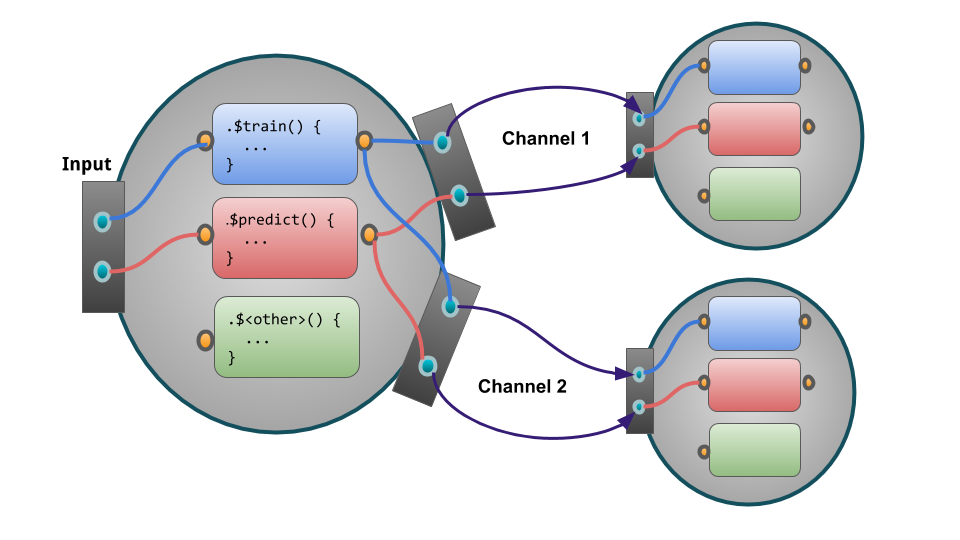
\includegraphics[width=0.98\linewidth]{images/po_multi_viz} \end{center}

\hypertarget{first-steps-inheriting-from-pipeop}{%
\subsubsection{\texorpdfstring{First Steps: Inheriting from \texttt{PipeOp}}{First Steps: Inheriting from PipeOp}}\label{first-steps-inheriting-from-pipeop}}

The first part of creating a custom \texttt{PipeOp} is inheriting from \texttt{PipeOp}.
We make a mental note that we need to implement a \texttt{train()} and a \texttt{predict()} function, and that we probably want to have an \texttt{initialize()} as well:

\begin{Shaded}
\begin{Highlighting}[]
\NormalTok{PipeOpCopyTwo =}\StringTok{ }\NormalTok{R6}\OperatorTok{::}\KeywordTok{R6Class}\NormalTok{(}\StringTok{"PipeOpCopyTwo"}\NormalTok{,}
  \DataTypeTok{inherit =}\NormalTok{ mlr3pipelines}\OperatorTok{::}\NormalTok{PipeOp,}
  \DataTypeTok{public =} \KeywordTok{list}\NormalTok{(}
    \DataTypeTok{initialize =} \ControlFlowTok{function}\NormalTok{(}\DataTypeTok{id =} \StringTok{"copy.two"}\NormalTok{) \{}
\NormalTok{      ....}
\NormalTok{    \},}

    \DataTypeTok{train =} \ControlFlowTok{function}\NormalTok{(inputs) \{}
\NormalTok{      ....}
\NormalTok{    \},}

    \DataTypeTok{predict =} \ControlFlowTok{function}\NormalTok{(inputs) \{}
\NormalTok{      ....}
\NormalTok{    \}}
\NormalTok{  )}
\NormalTok{)}
\end{Highlighting}
\end{Shaded}

\hypertarget{channel-definitions}{%
\subsubsection{Channel Definitions}\label{channel-definitions}}

We need to tell the \texttt{PipeOp} the layout of its channels: How many there are, what their names are going to be, and what types are acceptable.
This is done on initialization of the \texttt{PipeOp} (using a \texttt{super\$initialize} call) by giving the \texttt{input} and \texttt{output} \texttt{data.table} objects.
These must have three columns: a \texttt{"name"} column giving the names of input and output channels, and a \texttt{"train"} and \texttt{"predict"} column naming the class of objects we expect during training and prediction as input / output.
A special value for these classes is \texttt{"*"}, which indicates that any class will be accepted; our simple copy operator accepts any kind of input, so this will be useful. We have only one input, but two output channels.

By convention, we name a single channel \texttt{"input"} or \texttt{"output"}, and a group of channels {[}\texttt{"input1"}, \texttt{"input2"}, \ldots{}{]}, unless there is a reason to give specific different names. Therefore, our \texttt{input} \texttt{data.table} will have a single row \texttt{\textless{}"input",\ "*",\ "*"\textgreater{}}, and our \texttt{output} table will have two rows, \texttt{\textless{}"output1",\ "*",\ "*"\textgreater{}} and \texttt{\textless{}"output2",\ "*",\ "*"\textgreater{}}.

All of this is given to the \texttt{PipeOp} creator. Our \texttt{initialize()} will thus look as follows:

\begin{Shaded}
\begin{Highlighting}[]
\NormalTok{initialize =}\StringTok{ }\ControlFlowTok{function}\NormalTok{(}\DataTypeTok{id =} \StringTok{"copy.two"}\NormalTok{) \{}
\NormalTok{  input =}\StringTok{ }\NormalTok{data.table}\OperatorTok{::}\KeywordTok{data.table}\NormalTok{(}\DataTypeTok{name =} \StringTok{"input"}\NormalTok{, }\DataTypeTok{train =} \StringTok{"*"}\NormalTok{, }
    \DataTypeTok{predict =} \StringTok{"*"}\NormalTok{)}
  \CommentTok{# the following will create two rows and automatically}
  \CommentTok{# fill the `train` and `predict` cols with '*'}
\NormalTok{  output =}\StringTok{ }\NormalTok{data.table}\OperatorTok{::}\KeywordTok{data.table}\NormalTok{(}\DataTypeTok{name =} \KeywordTok{c}\NormalTok{(}\StringTok{"output1"}\NormalTok{, }\StringTok{"output2"}\NormalTok{), }
    \DataTypeTok{train =} \StringTok{"*"}\NormalTok{, }\DataTypeTok{predict =} \StringTok{"*"}\NormalTok{)}
\NormalTok{  super}\OperatorTok{$}\KeywordTok{initialize}\NormalTok{(id, }\DataTypeTok{input =}\NormalTok{ input, }\DataTypeTok{output =}\NormalTok{ output)}
\NormalTok{\}}
\end{Highlighting}
\end{Shaded}

\hypertarget{train-and-predict}{%
\subsubsection{Train and Predict}\label{train-and-predict}}

Both \texttt{train()} and \texttt{predict()} will receive a \texttt{list} as input and must give a \texttt{list} in return.
According to our \texttt{input} and \texttt{output} definitions, we will always get a list with a single element as input, and will need to return a list with two elements. Because all we want to do is create two copies, we will just create the copies using \texttt{c(inputs,\ inputs)}.

Two things to consider:

\begin{itemize}
\item
  The \texttt{train()} function must always modify the \texttt{self\$state} variable to something that is not \texttt{NULL} or \texttt{NO\_OP}.
  This is because the \texttt{\$state} slot is used as a signal that \texttt{PipeOp} has been trained on data, even if the state itself is not important to the \texttt{PipeOp} (as in our case).
  Therefore, our \texttt{train()} will set \texttt{self\$state\ =\ list()}.
\item
  It is not necessary to ``clone'' our input or make deep copies, because we don't modify the data.
  However, if we were changing a reference-passed object, for example by changing data in a \texttt{Task}, we would have to make a deep copy first.
  This is because a \texttt{PipeOp} may never modify its input object by reference.
\end{itemize}

Our \texttt{train()} and \texttt{predict()} functions are now:

\begin{Shaded}
\begin{Highlighting}[]
\NormalTok{train =}\StringTok{ }\ControlFlowTok{function}\NormalTok{(inputs) \{}
\NormalTok{  self}\OperatorTok{$}\NormalTok{state =}\StringTok{ }\KeywordTok{list}\NormalTok{()}
  \KeywordTok{c}\NormalTok{(inputs, inputs)}
\NormalTok{\}}
\end{Highlighting}
\end{Shaded}

\begin{Shaded}
\begin{Highlighting}[]
\NormalTok{predict =}\StringTok{ }\ControlFlowTok{function}\NormalTok{(inputs) \{}
  \KeywordTok{c}\NormalTok{(inputs, inputs)}
\NormalTok{\}}
\end{Highlighting}
\end{Shaded}

\hypertarget{putting-it-together}{%
\subsubsection{Putting it Together}\label{putting-it-together}}

The whole definition thus becomes

\begin{Shaded}
\begin{Highlighting}[]
\NormalTok{PipeOpCopyTwo =}\StringTok{ }\NormalTok{R6}\OperatorTok{::}\KeywordTok{R6Class}\NormalTok{(}\StringTok{"PipeOpCopyTwo"}\NormalTok{,}
  \DataTypeTok{inherit =}\NormalTok{ mlr3pipelines}\OperatorTok{::}\NormalTok{PipeOp,}
  \DataTypeTok{public =} \KeywordTok{list}\NormalTok{(}
    \DataTypeTok{initialize =} \ControlFlowTok{function}\NormalTok{(}\DataTypeTok{id =} \StringTok{"copy.two"}\NormalTok{) \{}
\NormalTok{      super}\OperatorTok{$}\KeywordTok{initialize}\NormalTok{(id,}
        \DataTypeTok{input =}\NormalTok{ data.table}\OperatorTok{::}\KeywordTok{data.table}\NormalTok{(}\DataTypeTok{name =} \StringTok{"input"}\NormalTok{, }\DataTypeTok{train =} \StringTok{"*"}\NormalTok{, }\DataTypeTok{predict =} \StringTok{"*"}\NormalTok{),}
        \DataTypeTok{output =}\NormalTok{ data.table}\OperatorTok{::}\KeywordTok{data.table}\NormalTok{(}\DataTypeTok{name =} \KeywordTok{c}\NormalTok{(}\StringTok{"output1"}\NormalTok{, }\StringTok{"output2"}\NormalTok{),}
                            \DataTypeTok{train =} \StringTok{"*"}\NormalTok{, }\DataTypeTok{predict =} \StringTok{"*"}\NormalTok{)}
\NormalTok{      )}
\NormalTok{    \},}

    \DataTypeTok{train =} \ControlFlowTok{function}\NormalTok{(inputs) \{}
\NormalTok{      self}\OperatorTok{$}\NormalTok{state =}\StringTok{ }\KeywordTok{list}\NormalTok{()}
      \KeywordTok{c}\NormalTok{(inputs, inputs)}
\NormalTok{    \},}

    \DataTypeTok{predict =} \ControlFlowTok{function}\NormalTok{(inputs) \{}
      \KeywordTok{c}\NormalTok{(inputs, inputs)}
\NormalTok{    \}}
\NormalTok{  )}
\NormalTok{)}
\end{Highlighting}
\end{Shaded}

We can create an instance of our \texttt{PipeOp}, put it in a graph, and see what happens when we train it on something:

\begin{Shaded}
\begin{Highlighting}[]
\KeywordTok{library}\NormalTok{(mlr3pipelines)}
\NormalTok{poct =}\StringTok{ }\NormalTok{PipeOpCopyTwo}\OperatorTok{$}\KeywordTok{new}\NormalTok{()}
\NormalTok{gr =}\StringTok{ }\NormalTok{Graph}\OperatorTok{$}\KeywordTok{new}\NormalTok{()}
\NormalTok{gr}\OperatorTok{$}\KeywordTok{add_pipeop}\NormalTok{(poct)}

\KeywordTok{print}\NormalTok{(gr)}
\NormalTok{## Graph with 1 PipeOps:}
\NormalTok{##        ID         State sccssors prdcssors}
\NormalTok{##  copy.two <<UNTRAINED>>}

\NormalTok{result =}\StringTok{ }\NormalTok{gr}\OperatorTok{$}\KeywordTok{train}\NormalTok{(task)}

\KeywordTok{str}\NormalTok{(result)}
\NormalTok{## List of 2}
\NormalTok{##  $ copy.two.output1:Classes 'TaskClassif', 'TaskSupervised', 'Task', 'R6' <TaskClassif:iris> }
\NormalTok{##  $ copy.two.output2:Classes 'TaskClassif', 'TaskSupervised', 'Task', 'R6' <TaskClassif:iris>}
\end{Highlighting}
\end{Shaded}

\hypertarget{ext-pipe-preproc}{%
\subsection{Special Case: Preprocessing}\label{ext-pipe-preproc}}

Many PipeOps perform an operation on exactly one \texttt{Task}, and return exactly one \texttt{Task}. They may even not care about the ``Target'' / ``Outcome'' variable of that task, and only do some modification of some input data.
However, it is usually important to them that the \texttt{Task} on which they perform prediction has the same data columns as the \texttt{Task} on which they train.
For these cases, the auxiliary base class \texttt{PipeOpTaskPreproc} exists.
It inherits from \texttt{PipeOp} itself, and other PipeOps should use it if they fall in the kind of use-case named above.

When inheriting from \texttt{PipeOpTaskPreproc}, one must either implement the \texttt{train\_task} and \texttt{predict\_task} functions, or the \texttt{train\_dt}, \texttt{predict\_dt} functions, depending on whether wants to operate on a \texttt{Task} object or on \texttt{data.table}s.
In the second case, one can optionally also overload the \texttt{select\_cols} function, which chooses which of the incoming \texttt{Task}'s features are given to the \texttt{train\_dt} / \texttt{predict\_dt} functions.

The following will show two examples: \texttt{PipeOpDropNA}, which removes a \texttt{Task}'s rows with missing values during training (and implements \texttt{train\_task} and \texttt{predict\_task}), and \texttt{PipeOpScale}, which scales a \texttt{Task}'s numeric columns (and implements \texttt{train\_dt}, \texttt{predict\_dt}, and \texttt{select\_cols}).

\hypertarget{example-pipeopdropna}{%
\subsubsection{\texorpdfstring{Example: \texttt{PipeOpDropNA}}{Example: PipeOpDropNA}}\label{example-pipeopdropna}}

Dropping rows with missing values may be important when training a model that can not handle them.

Because \href{https://mlr3.mlr-org.com}{mlr3} \texttt{Task}s only contain a view to the underlying data, it is not necessary to modify data to remove rows with missing values.
Instead, the rows can be removed using the \texttt{Task}'s \texttt{\$filter} method, which modifies the \texttt{Task} in-place.
This is done in the \texttt{train\_task} function. We take care that we also set the \texttt{\$state} slot to signal that the \texttt{PipeOp} was trained.

The \texttt{predict\_task} function does not need to do anything; removing missing values during prediction is not as useful, since learners that cannot handle them will just ignore the respective rows.
Furthermore, \href{https://mlr3.mlr-org.com}{mlr3} expects a \texttt{Learner} to always return just as many predictions as it was given input rows, so a \texttt{PipeOp} that removes \texttt{Task} rows during training can not be used inside a \texttt{GraphLearner}.

When we inherit from \texttt{PipeOpTaskPreproc}, it sets the \texttt{input} and \texttt{output} \texttt{data.table}s for us to only accept a single \texttt{Task}.
The only thing we do during \texttt{initialize()} is therefore to set an \texttt{id} (which can optionally be changed by the user).

The complete \texttt{PipeOpDropNA} can therefore be written as follows.
Note that it inherits from \texttt{PipeOpTaskPreproc}, unlike the \texttt{PipeOpCopyTwo} example from above:

\begin{Shaded}
\begin{Highlighting}[]
\NormalTok{PipeOpDropNA =}\StringTok{ }\NormalTok{R6}\OperatorTok{::}\KeywordTok{R6Class}\NormalTok{(}\StringTok{"PipeOpDropNA"}\NormalTok{,}
  \DataTypeTok{inherit =}\NormalTok{ mlr3pipelines}\OperatorTok{::}\NormalTok{PipeOpTaskPreproc,}
  \DataTypeTok{public =} \KeywordTok{list}\NormalTok{(}
    \DataTypeTok{initialize =} \ControlFlowTok{function}\NormalTok{(}\DataTypeTok{id =} \StringTok{"drop.na"}\NormalTok{) \{}
\NormalTok{      super}\OperatorTok{$}\KeywordTok{initialize}\NormalTok{(id)}
\NormalTok{    \},}

    \DataTypeTok{train_task =} \ControlFlowTok{function}\NormalTok{(task) \{}
\NormalTok{      self}\OperatorTok{$}\NormalTok{state =}\StringTok{ }\KeywordTok{list}\NormalTok{()}
\NormalTok{      featuredata =}\StringTok{ }\NormalTok{task}\OperatorTok{$}\KeywordTok{data}\NormalTok{(}\DataTypeTok{cols =}\NormalTok{ task}\OperatorTok{$}\NormalTok{feature_names)}
\NormalTok{      exclude =}\StringTok{ }\KeywordTok{apply}\NormalTok{(}\KeywordTok{is.na}\NormalTok{(featuredata), }\DecValTok{1}\NormalTok{, any)}
\NormalTok{      task}\OperatorTok{$}\KeywordTok{filter}\NormalTok{(task}\OperatorTok{$}\NormalTok{row_ids[}\OperatorTok{!}\NormalTok{exclude])}
\NormalTok{    \},}

    \DataTypeTok{predict_task =} \ControlFlowTok{function}\NormalTok{(task) \{}
      \CommentTok{# nothing to be done}
\NormalTok{      task}
\NormalTok{    \}}
\NormalTok{  )}
\NormalTok{)}
\end{Highlighting}
\end{Shaded}

To test this \texttt{PipeOp}, we create a small task with missing values:

\begin{Shaded}
\begin{Highlighting}[]
\NormalTok{smalliris =}\StringTok{ }\NormalTok{iris[(}\DecValTok{1}\OperatorTok{:}\DecValTok{5}\NormalTok{) }\OperatorTok{*}\StringTok{ }\DecValTok{30}\NormalTok{, ]}
\NormalTok{smalliris[}\DecValTok{1}\NormalTok{, }\DecValTok{1}\NormalTok{] =}\StringTok{ }\OtherTok{NA}
\NormalTok{smalliris[}\DecValTok{2}\NormalTok{, }\DecValTok{2}\NormalTok{] =}\StringTok{ }\OtherTok{NA}
\NormalTok{sitask =}\StringTok{ }\NormalTok{TaskClassif}\OperatorTok{$}\KeywordTok{new}\NormalTok{(}\StringTok{"smalliris"}\NormalTok{, }\KeywordTok{as_data_backend}\NormalTok{(smalliris), }
  \StringTok{"Species"}\NormalTok{)}
\KeywordTok{print}\NormalTok{(sitask}\OperatorTok{$}\KeywordTok{data}\NormalTok{())}
\NormalTok{##       Species Petal.Length Petal.Width Sepal.Length}
\NormalTok{## 1:     setosa          1.6         0.2           NA}
\NormalTok{## 2: versicolor          3.9         1.4          5.2}
\NormalTok{## 3: versicolor          4.0         1.3          5.5}
\NormalTok{## 4:  virginica          5.0         1.5          6.0}
\NormalTok{## 5:  virginica          5.1         1.8          5.9}
\NormalTok{##    Sepal.Width}
\NormalTok{## 1:         3.2}
\NormalTok{## 2:          NA}
\NormalTok{## 3:         2.5}
\NormalTok{## 4:         2.2}
\NormalTok{## 5:         3.0}
\end{Highlighting}
\end{Shaded}

We test this by feeding it to a new \texttt{Graph} that uses \texttt{PipeOpDropNA}.

\begin{Shaded}
\begin{Highlighting}[]
\NormalTok{gr =}\StringTok{ }\NormalTok{Graph}\OperatorTok{$}\KeywordTok{new}\NormalTok{()}
\NormalTok{gr}\OperatorTok{$}\KeywordTok{add_pipeop}\NormalTok{(PipeOpDropNA}\OperatorTok{$}\KeywordTok{new}\NormalTok{())}

\NormalTok{filtered_task =}\StringTok{ }\NormalTok{gr}\OperatorTok{$}\KeywordTok{train}\NormalTok{(sitask)[[}\DecValTok{1}\NormalTok{]]}
\KeywordTok{print}\NormalTok{(filtered_task}\OperatorTok{$}\KeywordTok{data}\NormalTok{())}
\NormalTok{##       Species Petal.Length Petal.Width Sepal.Length}
\NormalTok{## 1: versicolor          4.0         1.3          5.5}
\NormalTok{## 2:  virginica          5.0         1.5          6.0}
\NormalTok{## 3:  virginica          5.1         1.8          5.9}
\NormalTok{##    Sepal.Width}
\NormalTok{## 1:         2.5}
\NormalTok{## 2:         2.2}
\NormalTok{## 3:         3.0}
\end{Highlighting}
\end{Shaded}

\hypertarget{example-pipeopscalealways}{%
\subsubsection{\texorpdfstring{Example: \texttt{PipeOpScaleAlways}}{Example: PipeOpScaleAlways}}\label{example-pipeopscalealways}}

An often-applied preprocessing step is to simply \textbf{center} and/or \textbf{scale} the data to mean \(0\) and standard deviation \(1\).
This fits the \texttt{PipeOpTaskPreproc} pattern quite well.
Because it always replaces all columns that it operates on, and does not require any information about the task's target, it only needs to overload the \texttt{train\_dt} and \texttt{predict\_dt} functions.
This saves some boilerplate-code from getting the correct feature columns out of the task, and replacing them after modification.

Because scaling only makes sense on numeric features, we want to instruct \texttt{PipeOpTaskPreproc} to give us only these numeric columns.
We do this by overloading the \texttt{select\_cols} function: It is called by the class to determine which columns to give to \texttt{train\_dt} and \texttt{predict\_dt}.
Its input is the \texttt{Task} that is being transformed, and it should return a \texttt{character} vector of all features to work with.
When it is not overloaded, it uses all columns; instead, we will set it to only give us numeric columns.
Because the \texttt{levels()} of the data table given to \texttt{train\_dt} and \texttt{predict\_dt} may be different from the levels \texttt{task}'s levels, these functions must also take a \texttt{levels} argument that is a named list of column names indicating their levels.
When working with numeric data, this argument can be ignored, but it should be used instead of \texttt{levels(dt{[}{[}column{]}{]})} for factorial or character columns.

This is the first \texttt{PipeOp} where we will be using the \texttt{\$state} slot for something useful: We save the centering offset and scaling coefficient and use it in \texttt{\$predict()}!

For simplicity, we are not using hyperparameters and will always scale and center all data.
Compare this \texttt{PipeOpScaleAlways} operator to the one defined inside the \href{https://mlr3pipelines.mlr-org.com}{mlr3pipelines} package, \texttt{PipeOpScale}, defined in \texttt{PipeOpScale.R}.

\begin{Shaded}
\begin{Highlighting}[]
\NormalTok{PipeOpScaleAlways =}\StringTok{ }\NormalTok{R6}\OperatorTok{::}\KeywordTok{R6Class}\NormalTok{(}\StringTok{"PipeOpScaleAlways"}\NormalTok{,}
  \DataTypeTok{inherit =}\NormalTok{ mlr3pipelines}\OperatorTok{::}\NormalTok{PipeOpTaskPreproc,}
  \DataTypeTok{public =} \KeywordTok{list}\NormalTok{(}
    \DataTypeTok{initialize =} \ControlFlowTok{function}\NormalTok{(}\DataTypeTok{id =} \StringTok{"scale.always"}\NormalTok{) \{}
\NormalTok{      super}\OperatorTok{$}\KeywordTok{initialize}\NormalTok{(}\DataTypeTok{id =}\NormalTok{ id)}
\NormalTok{    \},}

    \DataTypeTok{select_cols =} \ControlFlowTok{function}\NormalTok{(task) \{}
\NormalTok{      task}\OperatorTok{$}\NormalTok{feature_types[type }\OperatorTok{==}\StringTok{ "numeric"}\NormalTok{, id]}
\NormalTok{    \},}

    \DataTypeTok{train_dt =} \ControlFlowTok{function}\NormalTok{(dt, levels, target) \{}
\NormalTok{      sc =}\StringTok{ }\KeywordTok{scale}\NormalTok{(}\KeywordTok{as.matrix}\NormalTok{(dt))}
\NormalTok{      self}\OperatorTok{$}\NormalTok{state =}\StringTok{ }\KeywordTok{list}\NormalTok{(}
        \DataTypeTok{center =} \KeywordTok{attr}\NormalTok{(sc, }\StringTok{"scaled:center"}\NormalTok{),}
        \DataTypeTok{scale =} \KeywordTok{attr}\NormalTok{(sc, }\StringTok{"scaled:scale"}\NormalTok{)}
\NormalTok{      )}
\NormalTok{      sc}
\NormalTok{    \},}

    \DataTypeTok{predict_dt =} \ControlFlowTok{function}\NormalTok{(dt, levels) \{}
      \KeywordTok{t}\NormalTok{((}\KeywordTok{t}\NormalTok{(dt) }\OperatorTok{-}\StringTok{ }\NormalTok{self}\OperatorTok{$}\NormalTok{state}\OperatorTok{$}\NormalTok{center) }\OperatorTok{/}\StringTok{ }\NormalTok{self}\OperatorTok{$}\NormalTok{state}\OperatorTok{$}\NormalTok{scale)}
\NormalTok{    \}}
\NormalTok{  )}
\NormalTok{)}
\end{Highlighting}
\end{Shaded}

\emph{(Note for the observant: If you check \texttt{PipeOpScale.R} from the \href{https://mlr3pipelines.mlr-org.com}{mlr3pipelines} package, you will notice that is uses ``\texttt{get("type}'' and ``\texttt{get("id}'' instead of ``\texttt{type}'' and ``\texttt{id}'', because the static code checker on CRAN would otherwise complain about references to undefined variables. This is a ``problem'' with \texttt{data.table} and not exclusive to \href{https://mlr3pipelines.mlr-org.com}{mlr3pipelines}.)}

We can, again, create a new \texttt{Graph} that uses this \texttt{PipeOp} to test it.
Compare the resulting data to the original ``iris'' \texttt{Task} data printed at the beginning:

\begin{Shaded}
\begin{Highlighting}[]
\NormalTok{gr =}\StringTok{ }\NormalTok{Graph}\OperatorTok{$}\KeywordTok{new}\NormalTok{()}
\NormalTok{gr}\OperatorTok{$}\KeywordTok{add_pipeop}\NormalTok{(PipeOpScaleAlways}\OperatorTok{$}\KeywordTok{new}\NormalTok{())}

\NormalTok{result =}\StringTok{ }\NormalTok{gr}\OperatorTok{$}\KeywordTok{train}\NormalTok{(task)}

\NormalTok{result[[}\DecValTok{1}\NormalTok{]]}\OperatorTok{$}\KeywordTok{data}\NormalTok{()}
\NormalTok{##        Species Petal.Length Petal.Width Sepal.Length}
\NormalTok{##   1:    setosa      -1.3358     -1.3111     -0.89767}
\NormalTok{##   2:    setosa      -1.3358     -1.3111     -1.13920}
\NormalTok{##   3:    setosa      -1.3924     -1.3111     -1.38073}
\NormalTok{##   4:    setosa      -1.2791     -1.3111     -1.50149}
\NormalTok{##   5:    setosa      -1.3358     -1.3111     -1.01844}
\NormalTok{##  ---                                                }
\NormalTok{## 146: virginica       0.8169      1.4440      1.03454}
\NormalTok{## 147: virginica       0.7036      0.9192      0.55149}
\NormalTok{## 148: virginica       0.8169      1.0504      0.79301}
\NormalTok{## 149: virginica       0.9302      1.4440      0.43072}
\NormalTok{## 150: virginica       0.7602      0.7880      0.06843}
\NormalTok{##      Sepal.Width}
\NormalTok{##   1:     1.01560}
\NormalTok{##   2:    -0.13154}
\NormalTok{##   3:     0.32732}
\NormalTok{##   4:     0.09789}
\NormalTok{##   5:     1.24503}
\NormalTok{##  ---            }
\NormalTok{## 146:    -0.13154}
\NormalTok{## 147:    -1.27868}
\NormalTok{## 148:    -0.13154}
\NormalTok{## 149:     0.78617}
\NormalTok{## 150:    -0.13154}
\end{Highlighting}
\end{Shaded}

\hypertarget{special-case-preprocessing-with-simple-train}{%
\subsection{Special Case: Preprocessing with Simple Train}\label{special-case-preprocessing-with-simple-train}}

It is possible to make even further simplifications for many \texttt{PipeOp}s that perform mostly the same operation during training and prediction.
The point of \texttt{Task} preprocessing is often to modify the training data in mostly the same way as prediction data (but in a way that \emph{may} depend on training data).

Consider constant feature removal, for example: The goal is to remove features that have no variance, or only a single factor level.
However, what features get removed must be decided during \emph{training}, and may only depend on training data.
Furthermore, the actual process of removing features is the same during training and prediction.

A simplification to make is therefore to have a function \texttt{get\_state(task)} which sets the \texttt{\$state} slot during training, and a \texttt{transform(task)} function, which gets called both during training \emph{and} prediction.
This is done in the \texttt{PipeOpTaskPreprocSimple} class.
Just like \texttt{PipeOpTaskPreproc}, one can inherit from this and overload these functions to get a \texttt{PipeOp} that performs preprocessing with very little boilerplate code.

Just like \texttt{PipeOpTaskPreproc}, \texttt{PipeOpTaskPreprocSimple} offers the possibility to instead overload the \texttt{get\_state\_dt(dt,\ levels)} and \texttt{transform\_dt(dt,\ levels)} functions (and optionally, again, the \texttt{select\_cols(task)} function) to operate on \texttt{data.table} feature data instead of the whole \texttt{Task}.

Even some methods that do not use \texttt{PipeOpTaskPreprocSimple} \emph{could} work in a similar way: The \texttt{PipeOpScaleAlways} example from above will be shown to also work with this paradigm.

\hypertarget{example-pipeopdropconst}{%
\subsubsection{\texorpdfstring{Example: \texttt{PipeOpDropConst}}{Example: PipeOpDropConst}}\label{example-pipeopdropconst}}

A typical example of a preprocessing operation that does almost the same operation during training and prediction is an operation that drops features depending on a criterion that is evaluated during training.
One simple example of this is dropping constant features.
Because the \href{https://mlr3.mlr-org.com}{mlr3} \texttt{Task} class offers a flexible view on underlying data, it is most efficient to drop columns from the task directly using its \texttt{\$select()} function, so the \texttt{get\_state\_dt(dt,\ levels)} / \texttt{transform\_dt(dt,\ levels)} functions will \emph{not} get used; instead we overload the \texttt{get\_state(task)} and \texttt{transform(task)} functions.

The \texttt{get\_state()} function's result is saved to the \texttt{\$state} slot, so we want to return something that is useful for dropping features.
We choose to save the names of all the columns that have nonzero variance.
For brevity, we use \texttt{length(unique(column))\ \textgreater{}\ 1} to check whether more than one distinct value is present; a more sophisticated version could have a tolerance parameter for numeric values that are very close to each other.

The \texttt{transform()} function is evaluated both during training \emph{and} prediction, and can rely on the \texttt{\$state} slot being present.
All it does here is call the \texttt{Task\$select} function with the columns we chose to keep.

The full \texttt{PipeOp} could be written as follows:

\begin{Shaded}
\begin{Highlighting}[]
\NormalTok{PipeOpDropConst =}\StringTok{ }\NormalTok{R6}\OperatorTok{::}\KeywordTok{R6Class}\NormalTok{(}\StringTok{"PipeOpDropConst"}\NormalTok{,}
  \DataTypeTok{inherit =}\NormalTok{ mlr3pipelines}\OperatorTok{::}\NormalTok{PipeOpTaskPreprocSimple,}
  \DataTypeTok{public =} \KeywordTok{list}\NormalTok{(}
    \DataTypeTok{initialize =} \ControlFlowTok{function}\NormalTok{(}\DataTypeTok{id =} \StringTok{"drop.const"}\NormalTok{) \{}
\NormalTok{      super}\OperatorTok{$}\KeywordTok{initialize}\NormalTok{(}\DataTypeTok{id =}\NormalTok{ id)}
\NormalTok{    \},}

    \DataTypeTok{get_state =} \ControlFlowTok{function}\NormalTok{(task) \{}
\NormalTok{      data =}\StringTok{ }\NormalTok{task}\OperatorTok{$}\KeywordTok{data}\NormalTok{(}\DataTypeTok{cols =}\NormalTok{ task}\OperatorTok{$}\NormalTok{feature_names)}
\NormalTok{      nonconst =}\StringTok{ }\KeywordTok{sapply}\NormalTok{(data, }\ControlFlowTok{function}\NormalTok{(column) }\KeywordTok{length}\NormalTok{(}\KeywordTok{unique}\NormalTok{(column)) }\OperatorTok{>}\StringTok{ }\DecValTok{1}\NormalTok{)}
      \KeywordTok{list}\NormalTok{(}\DataTypeTok{cnames =} \KeywordTok{colnames}\NormalTok{(data)[nonconst])}
\NormalTok{    \},}

    \DataTypeTok{transform =} \ControlFlowTok{function}\NormalTok{(task) \{}
\NormalTok{      task}\OperatorTok{$}\KeywordTok{select}\NormalTok{(self}\OperatorTok{$}\NormalTok{state}\OperatorTok{$}\NormalTok{cnames)}
\NormalTok{    \}}
\NormalTok{  )}
\NormalTok{)}
\end{Highlighting}
\end{Shaded}

This can be tested using the first five rows of the ``Iris'' \texttt{Task}, for which one feature (\texttt{"Petal.Width"}) is constant:

\begin{Shaded}
\begin{Highlighting}[]
\NormalTok{irishead =}\StringTok{ }\NormalTok{task}\OperatorTok{$}\KeywordTok{clone}\NormalTok{()}\OperatorTok{$}\KeywordTok{filter}\NormalTok{(}\DecValTok{1}\OperatorTok{:}\DecValTok{5}\NormalTok{)}
\NormalTok{irishead}\OperatorTok{$}\KeywordTok{data}\NormalTok{()}
\NormalTok{##    Species Petal.Length Petal.Width Sepal.Length}
\NormalTok{## 1:  setosa          1.4         0.2          5.1}
\NormalTok{## 2:  setosa          1.4         0.2          4.9}
\NormalTok{## 3:  setosa          1.3         0.2          4.7}
\NormalTok{## 4:  setosa          1.5         0.2          4.6}
\NormalTok{## 5:  setosa          1.4         0.2          5.0}
\NormalTok{##    Sepal.Width}
\NormalTok{## 1:         3.5}
\NormalTok{## 2:         3.0}
\NormalTok{## 3:         3.2}
\NormalTok{## 4:         3.1}
\NormalTok{## 5:         3.6}
\end{Highlighting}
\end{Shaded}

\begin{Shaded}
\begin{Highlighting}[]
\NormalTok{gr =}\StringTok{ }\NormalTok{Graph}\OperatorTok{$}\KeywordTok{new}\NormalTok{()}\OperatorTok{$}\KeywordTok{add_pipeop}\NormalTok{(PipeOpDropConst}\OperatorTok{$}\KeywordTok{new}\NormalTok{())}
\NormalTok{dropped_task =}\StringTok{ }\NormalTok{gr}\OperatorTok{$}\KeywordTok{train}\NormalTok{(irishead)[[}\DecValTok{1}\NormalTok{]]}

\NormalTok{dropped_task}\OperatorTok{$}\KeywordTok{data}\NormalTok{()}
\NormalTok{##    Species Petal.Length Sepal.Length Sepal.Width}
\NormalTok{## 1:  setosa          1.4          5.1         3.5}
\NormalTok{## 2:  setosa          1.4          4.9         3.0}
\NormalTok{## 3:  setosa          1.3          4.7         3.2}
\NormalTok{## 4:  setosa          1.5          4.6         3.1}
\NormalTok{## 5:  setosa          1.4          5.0         3.6}
\end{Highlighting}
\end{Shaded}

We can also see that the \texttt{\$state} was correctly set. Calling \texttt{\$predict()} with this graph, even with different data (the whole Iris \texttt{Task}!) will still drop the \texttt{"Petal.Width"} column, as it should.

\begin{Shaded}
\begin{Highlighting}[]
\NormalTok{gr}\OperatorTok{$}\NormalTok{pipeops}\OperatorTok{$}\NormalTok{drop.const}\OperatorTok{$}\NormalTok{state}
\NormalTok{## $cnames}
\NormalTok{## [1] "Petal.Length" "Sepal.Length" "Sepal.Width" }
\NormalTok{## }
\NormalTok{## $affected_cols}
\NormalTok{## [1] "Petal.Length" "Petal.Width"  "Sepal.Length"}
\NormalTok{## [4] "Sepal.Width" }
\NormalTok{## }
\NormalTok{## $intasklayout}
\NormalTok{##              id    type}
\NormalTok{## 1: Petal.Length numeric}
\NormalTok{## 2:  Petal.Width numeric}
\NormalTok{## 3: Sepal.Length numeric}
\NormalTok{## 4:  Sepal.Width numeric}
\NormalTok{## }
\NormalTok{## $outtasklayout}
\NormalTok{##              id    type}
\NormalTok{## 1: Petal.Length numeric}
\NormalTok{## 2: Sepal.Length numeric}
\NormalTok{## 3:  Sepal.Width numeric}
\end{Highlighting}
\end{Shaded}

\begin{Shaded}
\begin{Highlighting}[]
\NormalTok{dropped_predict =}\StringTok{ }\NormalTok{gr}\OperatorTok{$}\KeywordTok{predict}\NormalTok{(task)[[}\DecValTok{1}\NormalTok{]]}

\NormalTok{dropped_predict}\OperatorTok{$}\KeywordTok{data}\NormalTok{()}
\NormalTok{##        Species Petal.Length Sepal.Length Sepal.Width}
\NormalTok{##   1:    setosa          1.4          5.1         3.5}
\NormalTok{##   2:    setosa          1.4          4.9         3.0}
\NormalTok{##   3:    setosa          1.3          4.7         3.2}
\NormalTok{##   4:    setosa          1.5          4.6         3.1}
\NormalTok{##   5:    setosa          1.4          5.0         3.6}
\NormalTok{##  ---                                                }
\NormalTok{## 146: virginica          5.2          6.7         3.0}
\NormalTok{## 147: virginica          5.0          6.3         2.5}
\NormalTok{## 148: virginica          5.2          6.5         3.0}
\NormalTok{## 149: virginica          5.4          6.2         3.4}
\NormalTok{## 150: virginica          5.1          5.9         3.0}
\end{Highlighting}
\end{Shaded}

\hypertarget{example-pipeopscalealwayssimple}{%
\subsubsection{\texorpdfstring{Example: \texttt{PipeOpScaleAlwaysSimple}}{Example: PipeOpScaleAlwaysSimple}}\label{example-pipeopscalealwayssimple}}

This example will show how a \texttt{PipeOpTaskPreprocSimple} can be used when only working on feature data in form of a \texttt{data.table}.
Instead of calling the \texttt{scale()} function, the \texttt{center} and \texttt{scale} values are calculated directly and saved to the \texttt{\$state} slot.
The \texttt{transform\_dt} function will then perform the same operation during both training and prediction: subtract the \texttt{center} and divide by the \texttt{scale} value.
As in the \protect\hyperlink{example-pipeopscalealways}{\texttt{PipeOpScaleAlways} example above}, we use \texttt{select\_cols()} so that we only work on numeric columns.

\begin{Shaded}
\begin{Highlighting}[]
\NormalTok{PipeOpScaleAlwaysSimple =}\StringTok{ }\NormalTok{R6}\OperatorTok{::}\KeywordTok{R6Class}\NormalTok{(}\StringTok{"PipeOpScaleAlwaysSimple"}\NormalTok{,}
  \DataTypeTok{inherit =}\NormalTok{ mlr3pipelines}\OperatorTok{::}\NormalTok{PipeOpTaskPreprocSimple,}
  \DataTypeTok{public =} \KeywordTok{list}\NormalTok{(}
    \DataTypeTok{initialize =} \ControlFlowTok{function}\NormalTok{(}\DataTypeTok{id =} \StringTok{"scale.always.simple"}\NormalTok{) \{}
\NormalTok{      super}\OperatorTok{$}\KeywordTok{initialize}\NormalTok{(}\DataTypeTok{id =}\NormalTok{ id)}
\NormalTok{    \},}

    \DataTypeTok{select_cols =} \ControlFlowTok{function}\NormalTok{(task) \{}
\NormalTok{      task}\OperatorTok{$}\NormalTok{feature_types[type }\OperatorTok{==}\StringTok{ "numeric"}\NormalTok{, id]}
\NormalTok{    \},}

    \DataTypeTok{get_state_dt =} \ControlFlowTok{function}\NormalTok{(dt, levels, target) \{}
      \KeywordTok{list}\NormalTok{(}
        \DataTypeTok{center =} \KeywordTok{sapply}\NormalTok{(dt, mean),}
        \DataTypeTok{scale =} \KeywordTok{sapply}\NormalTok{(dt, sd)}
\NormalTok{      )}
\NormalTok{    \},}

    \DataTypeTok{transform_dt =} \ControlFlowTok{function}\NormalTok{(dt, levels) \{}
      \KeywordTok{t}\NormalTok{((}\KeywordTok{t}\NormalTok{(dt) }\OperatorTok{-}\StringTok{ }\NormalTok{self}\OperatorTok{$}\NormalTok{state}\OperatorTok{$}\NormalTok{center) }\OperatorTok{/}\StringTok{ }\NormalTok{self}\OperatorTok{$}\NormalTok{state}\OperatorTok{$}\NormalTok{scale)}
\NormalTok{    \}}
\NormalTok{  )}
\NormalTok{)}
\end{Highlighting}
\end{Shaded}

We can compare this \texttt{PipeOp} to the one above to show that it behaves the same.

\begin{Shaded}
\begin{Highlighting}[]
\NormalTok{gr =}\StringTok{ }\NormalTok{Graph}\OperatorTok{$}\KeywordTok{new}\NormalTok{()}\OperatorTok{$}\KeywordTok{add_pipeop}\NormalTok{(PipeOpScaleAlways}\OperatorTok{$}\KeywordTok{new}\NormalTok{())}
\NormalTok{result_posa =}\StringTok{ }\NormalTok{gr}\OperatorTok{$}\KeywordTok{train}\NormalTok{(task)[[}\DecValTok{1}\NormalTok{]]}

\NormalTok{gr =}\StringTok{ }\NormalTok{Graph}\OperatorTok{$}\KeywordTok{new}\NormalTok{()}\OperatorTok{$}\KeywordTok{add_pipeop}\NormalTok{(PipeOpScaleAlwaysSimple}\OperatorTok{$}\KeywordTok{new}\NormalTok{())}
\NormalTok{result_posa_simple =}\StringTok{ }\NormalTok{gr}\OperatorTok{$}\KeywordTok{train}\NormalTok{(task)[[}\DecValTok{1}\NormalTok{]]}
\end{Highlighting}
\end{Shaded}

\begin{Shaded}
\begin{Highlighting}[]
\NormalTok{result_posa}\OperatorTok{$}\KeywordTok{data}\NormalTok{()}
\NormalTok{##        Species Petal.Length Petal.Width Sepal.Length}
\NormalTok{##   1:    setosa      -1.3358     -1.3111     -0.89767}
\NormalTok{##   2:    setosa      -1.3358     -1.3111     -1.13920}
\NormalTok{##   3:    setosa      -1.3924     -1.3111     -1.38073}
\NormalTok{##   4:    setosa      -1.2791     -1.3111     -1.50149}
\NormalTok{##   5:    setosa      -1.3358     -1.3111     -1.01844}
\NormalTok{##  ---                                                }
\NormalTok{## 146: virginica       0.8169      1.4440      1.03454}
\NormalTok{## 147: virginica       0.7036      0.9192      0.55149}
\NormalTok{## 148: virginica       0.8169      1.0504      0.79301}
\NormalTok{## 149: virginica       0.9302      1.4440      0.43072}
\NormalTok{## 150: virginica       0.7602      0.7880      0.06843}
\NormalTok{##      Sepal.Width}
\NormalTok{##   1:     1.01560}
\NormalTok{##   2:    -0.13154}
\NormalTok{##   3:     0.32732}
\NormalTok{##   4:     0.09789}
\NormalTok{##   5:     1.24503}
\NormalTok{##  ---            }
\NormalTok{## 146:    -0.13154}
\NormalTok{## 147:    -1.27868}
\NormalTok{## 148:    -0.13154}
\NormalTok{## 149:     0.78617}
\NormalTok{## 150:    -0.13154}
\end{Highlighting}
\end{Shaded}

\begin{Shaded}
\begin{Highlighting}[]
\NormalTok{result_posa_simple}\OperatorTok{$}\KeywordTok{data}\NormalTok{()}
\NormalTok{##        Species Petal.Length Petal.Width Sepal.Length}
\NormalTok{##   1:    setosa      -1.3358     -1.3111     -0.89767}
\NormalTok{##   2:    setosa      -1.3358     -1.3111     -1.13920}
\NormalTok{##   3:    setosa      -1.3924     -1.3111     -1.38073}
\NormalTok{##   4:    setosa      -1.2791     -1.3111     -1.50149}
\NormalTok{##   5:    setosa      -1.3358     -1.3111     -1.01844}
\NormalTok{##  ---                                                }
\NormalTok{## 146: virginica       0.8169      1.4440      1.03454}
\NormalTok{## 147: virginica       0.7036      0.9192      0.55149}
\NormalTok{## 148: virginica       0.8169      1.0504      0.79301}
\NormalTok{## 149: virginica       0.9302      1.4440      0.43072}
\NormalTok{## 150: virginica       0.7602      0.7880      0.06843}
\NormalTok{##      Sepal.Width}
\NormalTok{##   1:     1.01560}
\NormalTok{##   2:    -0.13154}
\NormalTok{##   3:     0.32732}
\NormalTok{##   4:     0.09789}
\NormalTok{##   5:     1.24503}
\NormalTok{##  ---            }
\NormalTok{## 146:    -0.13154}
\NormalTok{## 147:    -1.27868}
\NormalTok{## 148:    -0.13154}
\NormalTok{## 149:     0.78617}
\NormalTok{## 150:    -0.13154}
\end{Highlighting}
\end{Shaded}

\hypertarget{ext-pipe-hyperpars}{%
\subsection{Hyperparameters}\label{ext-pipe-hyperpars}}

\href{https://mlr3pipelines.mlr-org.com}{mlr3pipelines} uses the \href{https://paradox.mlr-org.com}{paradox} package to define parameter spaces for \texttt{PipeOp}s.
Parameters for \texttt{PipeOp}s can modify their behavior in certain ways, e.g.~switch centering or scaling off in the \texttt{PipeOpScale} operator.
The unified interface makes it possible to have parameters for whole \texttt{Graph}s that modify the individual \texttt{PipeOp}'s behavior.
The \texttt{Graph}s, when encapsulated in \texttt{GraphLearner}s, can even be tuned using the tuning functionality in \href{https://mlr3tuning.mlr-org.com}{mlr3tuning}.

Hyperparameters are declared during initialization, when calling the \texttt{PipeOp}'s \texttt{\$initialize()} function, by giving a \texttt{param\_set} argument.
The \texttt{param\_set} must be a \texttt{ParamSet} from the \href{https://paradox.mlr-org.com}{paradox} package; see the \href{https://mlr3book.mlr-org.com}{mlr3book} for more information on how to define parameter spaces.
After construction, the \texttt{ParamSet} can be accessed through the \texttt{\$param\_set} slot.
While it is \emph{possible} to modify this \texttt{ParamSet}, using e.g.~the \texttt{\$add()} and \texttt{\$add\_dep()} functions, \emph{after} adding it to the \texttt{PipeOp}, it is strongly advised against.

Hyperparameters can be set and queried through the \texttt{\$values} slot.
When setting hyperparameters, they are automatically checked to satisfy all conditions set by the \texttt{\$param\_set}, so it is not necessary to type check them.
Be aware that it is always possible to \emph{remove} hyperparameter values.

When a \texttt{PipeOp} is initialized, it usually does not have any parameter values---\texttt{\$values} takes the value \texttt{list()}.
It is possible to set initial parameter values in the \texttt{\$initialize()} constructor; this must be done \emph{after} the \texttt{super\$initialize()} call where the corresponding \texttt{ParamSet} must be supplied.
This is because setting \texttt{\$values} checks against the current \texttt{\$param\_set}, which would fail if the \texttt{\$param\_set} was not set yet.

When using an underlying library function (the \texttt{scale} function in \texttt{PipeOpScale}, say), then there is usually a ``default'' behavior of that function when a parameter is not given.
It is good practice to use this default behavior whenever a parameter is not set (or when it was removed).
This can easily be done when using the \href{https://mlr3misc.mlr-org.com}{mlr3misc} library's \texttt{invoke()} function, which has functionality similar to \texttt{base::do.call()}.

\hypertarget{hyperparameter-example-pipeopscale}{%
\subsubsection{\texorpdfstring{Hyperparameter Example: \texttt{PipeOpScale}}{Hyperparameter Example: PipeOpScale}}\label{hyperparameter-example-pipeopscale}}

How to use hyperparameters can best be shown through the example of \texttt{PipeOpScale}, which is very similar to the example above, \texttt{PipeOpScaleAlways}.
The difference is made by the presence of hyperparameters. \texttt{PipeOpScale} constructs a \texttt{ParamSet} in its \texttt{\$initialize} function and passes this on to the \texttt{super\$initialize} function:

\begin{Shaded}
\begin{Highlighting}[]
\NormalTok{PipeOpScale}\OperatorTok{$}\NormalTok{public_methods}\OperatorTok{$}\NormalTok{initialize}
\NormalTok{## function (id = "scale", param_vals = list()) }
\NormalTok{## \{}
\NormalTok{##     ps = ParamSet$new(params = list(ParamLgl$new("center", default = TRUE, }
\NormalTok{##         tags = c("train", "scale")), ParamLgl$new("scale", default = TRUE, }
\NormalTok{##         tags = c("train", "scale"))))}
\NormalTok{##     super$initialize(id = id, param_set = ps, param_vals = param_vals)}
\NormalTok{## \}}
\NormalTok{## <bytecode: 0x1968a1d0>}
\NormalTok{## <environment: namespace:mlr3pipelines>}
\end{Highlighting}
\end{Shaded}

The user has access to this and can set and get parameters. Types are automatically checked:

\begin{Shaded}
\begin{Highlighting}[]
\NormalTok{pss =}\StringTok{ }\NormalTok{PipeOpScale}\OperatorTok{$}\KeywordTok{new}\NormalTok{()}
\KeywordTok{print}\NormalTok{(pss}\OperatorTok{$}\NormalTok{param_set)}
\NormalTok{## ParamSet: scale}
\NormalTok{##                id    class lower upper      levels}
\NormalTok{## 1:         center ParamLgl    NA    NA  TRUE,FALSE}
\NormalTok{## 2:          scale ParamLgl    NA    NA  TRUE,FALSE}
\NormalTok{## 3: affect_columns ParamUty    NA    NA            }
\NormalTok{##        default value}
\NormalTok{## 1:        TRUE      }
\NormalTok{## 2:        TRUE      }
\NormalTok{## 3: <NoDefault>}
\end{Highlighting}
\end{Shaded}

\begin{Shaded}
\begin{Highlighting}[]
\NormalTok{pss}\OperatorTok{$}\NormalTok{param_set}\OperatorTok{$}\NormalTok{values}\OperatorTok{$}\NormalTok{center =}\StringTok{ }\OtherTok{FALSE}
\KeywordTok{print}\NormalTok{(pss}\OperatorTok{$}\NormalTok{param_set}\OperatorTok{$}\NormalTok{values)}
\NormalTok{## $center}
\NormalTok{## [1] FALSE}
\end{Highlighting}
\end{Shaded}

\begin{Shaded}
\begin{Highlighting}[]
\NormalTok{pss}\OperatorTok{$}\NormalTok{param_set}\OperatorTok{$}\NormalTok{values}\OperatorTok{$}\NormalTok{scale =}\StringTok{ "TRUE"}  \CommentTok{# bad input is checked!}
\NormalTok{## Error in (function (xs) : Assertion on 'xs' failed: scale: Must be of type 'logical flag', not 'character'.}
\end{Highlighting}
\end{Shaded}

How \texttt{PipeOpScale} handles its parameters can be seen in its \texttt{\$train} method: It gets the relevant parameters from its \texttt{\$values} slot and uses them in the \texttt{mlr3misc::invoke} call.
This has the advantage over calling \texttt{scale()} directly that if a parameter is not given, its default value from the \texttt{base::scale} function will be used.

\begin{Shaded}
\begin{Highlighting}[]
\NormalTok{PipeOpScale}\OperatorTok{$}\NormalTok{public_methods}\OperatorTok{$}\NormalTok{train}
\NormalTok{## function (dt, levels, target) }
\NormalTok{## \{}
\NormalTok{##     sc = invoke(scale, as.matrix(dt), .args = self$param_set$get_values(tags = "scale"))}
\NormalTok{##     self$state = list(center = attr(sc, "scaled:center") %??% }
\NormalTok{##         0, scale = attr(sc, "scaled:scale") %??% 1)}
\NormalTok{##     constfeat = self$state$scale == 0}
\NormalTok{##     self$state$scale[constfeat] = 1}
\NormalTok{##     sc[, constfeat] = 0}
\NormalTok{##     sc}
\NormalTok{## \}}
\NormalTok{## <bytecode: 0x19687d38>}
\NormalTok{## <environment: namespace:mlr3pipelines>}
\end{Highlighting}
\end{Shaded}

Another change that is necessary compared to \texttt{PipeOpScaleAlways} is that the attributes \texttt{"scaled:scale"} and \texttt{"scaled:center"} are not always present, depending on parameters, and possibly need to be set to default values \(1\) or \(0\), respectively.

It is now even possible (if a bit pointless) to call \texttt{PipeOpScale} with both \texttt{scale} and \texttt{center} set to \texttt{FALSE}, which returns the original dataset, unchanged.

\begin{Shaded}
\begin{Highlighting}[]
\NormalTok{pss}\OperatorTok{$}\NormalTok{param_set}\OperatorTok{$}\NormalTok{values}\OperatorTok{$}\NormalTok{scale =}\StringTok{ }\OtherTok{FALSE}
\NormalTok{pss}\OperatorTok{$}\NormalTok{param_set}\OperatorTok{$}\NormalTok{values}\OperatorTok{$}\NormalTok{center =}\StringTok{ }\OtherTok{FALSE}

\NormalTok{gr =}\StringTok{ }\NormalTok{Graph}\OperatorTok{$}\KeywordTok{new}\NormalTok{()}
\NormalTok{gr}\OperatorTok{$}\KeywordTok{add_pipeop}\NormalTok{(pss)}

\NormalTok{result =}\StringTok{ }\NormalTok{gr}\OperatorTok{$}\KeywordTok{train}\NormalTok{(task)}

\NormalTok{result[[}\DecValTok{1}\NormalTok{]]}\OperatorTok{$}\KeywordTok{data}\NormalTok{()}
\NormalTok{##        Species Petal.Length Petal.Width Sepal.Length}
\NormalTok{##   1:    setosa          1.4         0.2          5.1}
\NormalTok{##   2:    setosa          1.4         0.2          4.9}
\NormalTok{##   3:    setosa          1.3         0.2          4.7}
\NormalTok{##   4:    setosa          1.5         0.2          4.6}
\NormalTok{##   5:    setosa          1.4         0.2          5.0}
\NormalTok{##  ---                                                }
\NormalTok{## 146: virginica          5.2         2.3          6.7}
\NormalTok{## 147: virginica          5.0         1.9          6.3}
\NormalTok{## 148: virginica          5.2         2.0          6.5}
\NormalTok{## 149: virginica          5.4         2.3          6.2}
\NormalTok{## 150: virginica          5.1         1.8          5.9}
\NormalTok{##      Sepal.Width}
\NormalTok{##   1:         3.5}
\NormalTok{##   2:         3.0}
\NormalTok{##   3:         3.2}
\NormalTok{##   4:         3.1}
\NormalTok{##   5:         3.6}
\NormalTok{##  ---            }
\NormalTok{## 146:         3.0}
\NormalTok{## 147:         2.5}
\NormalTok{## 148:         3.0}
\NormalTok{## 149:         3.4}
\NormalTok{## 150:         3.0}
\end{Highlighting}
\end{Shaded}

\hypertarget{special-tasks}{%
\chapter{Special Tasks}\label{special-tasks}}

This chapter explores the different functions of \href{https://mlr3.mlr-org.com}{mlr3} when dealing with specific data sets that require further statistical modification to undertake sensible analysis.
Following topics are discussed:

\textbf{Survival Analysis}

This sub-chapter explains how to conduct sound \protect\hyperlink{survival}{survival analysis} in mlr3.
\protect\hyperlink{survival}{Survival analysis} is used to monitor the period of time until a specific event takes places.
This specific event could be e.g.~death, transmission of a disease, marriage or divorce.
Two considerations are important when conducting \protect\hyperlink{survival}{survival analysis}:

\begin{itemize}
\tightlist
\item
  Whether the event occurred within the frame of the given data
\item
  How much time it took until the event occurred
\end{itemize}

In summary, this sub-chapter explains how to account for these considerations and conduct survival analysis using the \href{https://mlr3proba.mlr-org.com}{mlr3proba} extension package.

\textbf{Spatial Analysis}

\protect\hyperlink{spatial}{Spatial analysis} data observations entail reference information about spatial characteristics.
One of the largest shortcomings of \protect\hyperlink{spatial}{spatial data analysis} is the inevitable auto-correlation in spatial data.
Auto-correlation is especially severe in data with marginal spatial variation.
The sub-chapter on \protect\hyperlink{spatial}{spatial analysis} provides instructions on how to handle the problems associated with spatial data accordingly.

\textbf{Ordinal Analysis}

This is work in progress.
See \texttt{mlr-org/mlr3ordinal} for the current state.

\textbf{Functional Analysis}

\protect\hyperlink{functional}{Functional analysis} contains data that consists of curves varying over a continuum e.g.~time, frequency or wavelength.
This type of analysis is frequently used when examining measurements over various time points.
Steps on how to accommodate functional data structures in mlr3 are explained in the \protect\hyperlink{functional}{functional analysis} sub-chapter.

\textbf{Multilabel Classification}

\protect\hyperlink{multilabel}{Multilabel classification} deals with objects that can belong to more than one category at the same time.
Numerous target labels are attributed to a single observation.
Working with multilabel data requires one to use modified algorithms, to accommodate data specific characteristics.
Two approaches to \protect\hyperlink{multilabel}{multilabel classification} are prominently used:

\begin{itemize}
\tightlist
\item
  The problem transformation method
\item
  The algorithm adaption method
\end{itemize}

Instructions on how to deal with \protect\hyperlink{multilabel}{multilabel classification} in mlr3 can be found in this sub-chapter.

\textbf{Cost Sensitive Classification}

This sub-chapter deals with the implementation of \protect\hyperlink{cost-sens}{cost-sensitive classification}.
Regular classification aims to minimize the misclassification rate and thus all types of misclassification errors are deemed equally severe.
\protect\hyperlink{cost-sens}{Cost-sensitive classification} is a setting where the costs caused by different kinds of errors are not assumed to be equal.
The objective is to minimize the expected costs.

Analytical data for a big credit institution is used as a use case to illustrate the different features.
Firstly, the sub-chapter provides guidance on how to implement a first model.
Subsequently, the sub-chapter contains instructions on how to modify cost sensitivity measures, thresholding and threshold tuning.

\hypertarget{survival}{%
\section{Survival Analysis}\label{survival}}

Survival analysis examines data on whether a specific event of interest takes place and how long it takes till this event occurs.
One cannot use ordinary regression analysis when dealing with survival analysis data sets.
Firstly, survival data contains solely positive values and therefore needs to be transformed to avoid biases.
Secondly, ordinary regression analysis cannot deal with censored observations accordingly.
Censored observations are observations in which the event of interest has not occurred, yet.
Survival analysis allows the user to handle censored data with limited time frames that sometimes do not entail the event of interest.
Note that survival analysis accounts for both censored and uncensored observations while adjusting respective model parameters.

The package \href{https://mlr3proba.mlr-org.com}{mlr3proba} extends \href{https://mlr3.mlr-org.com}{mlr3} with the following objects for survival analysis:

\begin{itemize}
\tightlist
\item
  \texttt{mlr3proba::TaskSurv",\ text\ =\ "TaskSurv} to define (right-censored) survival tasks
\item
  \texttt{mlr3proba::LearnerSurv",\ text\ =\ "LearnerSurv} as base class for survival learners
\item
  \texttt{mlr3proba::PredictionSurv",\ text\ =\ "PredictionSurv} as specialized class for \texttt{Prediction} objects
\item
  \texttt{mlr3proba::MeasureSurv",\ text\ =\ "MeasureSurv} as specialized class for performance measures
\end{itemize}

In this example we demonstrate the basic functionality of the package on the \texttt{survival::rats",\ text\ =\ "rats} data from the \texttt{survival} package.
This task ships as pre-defined \texttt{TaskSurv} with \href{https://mlr3proba.mlr-org.com}{mlr3proba}.

\begin{Shaded}
\begin{Highlighting}[]
\KeywordTok{library}\NormalTok{(mlr3proba)}
\NormalTok{task =}\StringTok{ }\KeywordTok{tsk}\NormalTok{(}\StringTok{"rats"}\NormalTok{)}
\KeywordTok{print}\NormalTok{(task)}
\NormalTok{## <TaskSurv:rats> (300 x 5)}
\NormalTok{## * Target: time, status}
\NormalTok{## * Properties: -}
\NormalTok{## * Features (3):}
\NormalTok{##   - int (2): litter, rx}
\NormalTok{##   - fct (1): sex}

\CommentTok{# the target column is a survival object:}
\KeywordTok{head}\NormalTok{(task}\OperatorTok{$}\KeywordTok{truth}\NormalTok{())}
\NormalTok{## [1] 101+  49  104+  91+ 104+ 102+}
\end{Highlighting}
\end{Shaded}

Now, we conduct a small benchmark study on the \texttt{mlr\_tasks\_rats",\ text\ =\ "rats} task using some of the integrated survival learners:

\begin{Shaded}
\begin{Highlighting}[]
\CommentTok{# integrated learners}
\NormalTok{learners =}\StringTok{ }\KeywordTok{lapply}\NormalTok{(}\KeywordTok{c}\NormalTok{(}\StringTok{"surv.coxph"}\NormalTok{, }\StringTok{"surv.kaplan"}\NormalTok{, }\StringTok{"surv.ranger"}\NormalTok{), }
\NormalTok{  lrn)}
\KeywordTok{print}\NormalTok{(learners)}
\NormalTok{## [[1]]}
\NormalTok{## <LearnerSurvCoxPH:surv.coxph>}
\NormalTok{## * Model: -}
\NormalTok{## * Parameters: list()}
\NormalTok{## * Packages: survival, distr6}
\NormalTok{## * Predict Type: distr}
\NormalTok{## * Feature types: logical, integer, numeric,}
\NormalTok{##   factor}
\NormalTok{## * Properties: importance}
\NormalTok{## }
\NormalTok{## [[2]]}
\NormalTok{## <LearnerSurvKaplan:surv.kaplan>}
\NormalTok{## * Model: -}
\NormalTok{## * Parameters: list()}
\NormalTok{## * Packages: survival, distr6}
\NormalTok{## * Predict Type: crank}
\NormalTok{## * Feature types: logical, integer, numeric,}
\NormalTok{##   character, factor, ordered}
\NormalTok{## * Properties: missings}
\NormalTok{## }
\NormalTok{## [[3]]}
\NormalTok{## <LearnerSurvRanger:surv.ranger>}
\NormalTok{## * Model: -}
\NormalTok{## * Parameters: list()}
\NormalTok{## * Packages: ranger, distr6}
\NormalTok{## * Predict Type: distr}
\NormalTok{## * Feature types: logical, integer, numeric,}
\NormalTok{##   character, factor, ordered}
\NormalTok{## * Properties: importance, oob_error, weights}

\NormalTok{measure =}\StringTok{ }\KeywordTok{msr}\NormalTok{(}\StringTok{"surv.harrellC"}\NormalTok{)}
\KeywordTok{print}\NormalTok{(measure)}
\NormalTok{## <MeasureSurvHarrellC:surv.harrellC>}
\NormalTok{## * Packages: -}
\NormalTok{## * Range: [0, 1]}
\NormalTok{## * Minimize: FALSE}
\NormalTok{## * Properties: -}
\NormalTok{## * Predict type: crank}

\KeywordTok{set.seed}\NormalTok{(}\DecValTok{1}\NormalTok{)}
\NormalTok{bmr =}\StringTok{ }\KeywordTok{benchmark}\NormalTok{(}\KeywordTok{benchmark_grid}\NormalTok{(task, learners, }\KeywordTok{rsmp}\NormalTok{(}\StringTok{"cv"}\NormalTok{, }
  \DataTypeTok{folds =} \DecValTok{3}\NormalTok{)))}
\KeywordTok{print}\NormalTok{(bmr)}
\NormalTok{## <BenchmarkResult> of 9 rows with 3 resampling runs}
\NormalTok{##  nr task_id  learner_id resampling_id iters warnings}
\NormalTok{##   1    rats  surv.coxph            cv     3        0}
\NormalTok{##   2    rats surv.kaplan            cv     3        0}
\NormalTok{##   3    rats surv.ranger            cv     3        0}
\NormalTok{##  errors}
\NormalTok{##       0}
\NormalTok{##       0}
\NormalTok{##       0}
\end{Highlighting}
\end{Shaded}

\hypertarget{spatial}{%
\section{Spatial Analysis}\label{spatial}}

Spatial data observations entail reference information about spatial characteristics.
This information is frequently stored as coordinates named `x' and `y'.
Treating spatial data using non-spatial data methods could lead to over-optimistic treatment.
This is due to the underlying auto-correlation in spatial data.

See \texttt{mlr-org/mlr3spatiotemporal} for the current state of the implementation.

\hypertarget{ordinal}{%
\section{Ordinal Analysis}\label{ordinal}}

This is work in progress.
See \texttt{mlr-org/mlr3ordinal} for the current state of the implementation.

\hypertarget{functional}{%
\section{Functional Analysis}\label{functional}}

Functional data is data containing an ordering on the dimensions.
This implies that functional data consists of curves varying over a continuum, such as time, frequency, or wavelength.

\hypertarget{how-to-model-functional-data}{%
\subsection{How to model functional data?}\label{how-to-model-functional-data}}

There are two ways to model functional data:

\begin{itemize}
\tightlist
\item
  Modification of the learner, so that the learner is suitable for the functional data
\item
  Modification of the task, so that the task matches the standard- or classification-learner
\end{itemize}

More following soon!

\hypertarget{multilabel}{%
\section{Multilabel Classification}\label{multilabel}}

Multilabel deals with objects that can belong to more than one category at the same time.

More following soon!

\hypertarget{cost-sens}{%
\section{Cost-Sensitive Classification}\label{cost-sens}}

In regular classification the aim is to minimize the misclassification rate and thus all types of misclassification errors are deemed equally severe.
A more general setting is cost-sensitive classification.
Cost sensitive classification does not assume that the costs caused by different kinds of errors are equal.
The objective of cost sensitive classification is to minimize the expected costs.

Imagine you are an analyst for a big credit institution.
Let's also assume that a correct decision of the bank would result in 35\% of the profit at the end of a specific period.
A correct decision means that the bank predicts that a customer will pay their bills (hence would obtain a loan), and the customer indeed has good credit.
On the other hand, a wrong decision means that the bank predicts that the customer's credit is in good standing, but the opposite is true.
This would result in a loss of 100\% of the given loan.

\begin{longtable}[]{@{}ccc@{}}
\toprule
& Good Customer (truth) & Bad Customer (truth)\tabularnewline
\midrule
\endhead
Good Customer (predicted) & + 0.35 & - 1.0\tabularnewline
Bad Customer (predicted) & 0 & 0\tabularnewline
\bottomrule
\end{longtable}

Expressed as costs (instead of profit), we can write down the cost-matrix as follows:

\begin{Shaded}
\begin{Highlighting}[]
\NormalTok{costs =}\StringTok{ }\KeywordTok{matrix}\NormalTok{(}\KeywordTok{c}\NormalTok{(}\OperatorTok{-}\FloatTok{0.35}\NormalTok{, }\DecValTok{0}\NormalTok{, }\DecValTok{1}\NormalTok{, }\DecValTok{0}\NormalTok{), }\DataTypeTok{nrow =} \DecValTok{2}\NormalTok{)}
\KeywordTok{dimnames}\NormalTok{(costs) =}\StringTok{ }\KeywordTok{list}\NormalTok{(}\DataTypeTok{response =} \KeywordTok{c}\NormalTok{(}\StringTok{"good"}\NormalTok{, }\StringTok{"bad"}\NormalTok{), }\DataTypeTok{truth =} \KeywordTok{c}\NormalTok{(}\StringTok{"good"}\NormalTok{, }
  \StringTok{"bad"}\NormalTok{))}
\KeywordTok{print}\NormalTok{(costs)}
\NormalTok{##         truth}
\NormalTok{## response  good bad}
\NormalTok{##     good -0.35   1}
\NormalTok{##     bad   0.00   0}
\end{Highlighting}
\end{Shaded}

An exemplary data set for such a problem is the \texttt{mlr\_tasks\_german\_credit",\ text\ =\ "German\ Credit} task:

\begin{Shaded}
\begin{Highlighting}[]
\KeywordTok{library}\NormalTok{(mlr3)}
\NormalTok{task =}\StringTok{ }\KeywordTok{tsk}\NormalTok{(}\StringTok{"german_credit"}\NormalTok{)}
\KeywordTok{table}\NormalTok{(task}\OperatorTok{$}\KeywordTok{truth}\NormalTok{())}
\NormalTok{## }
\NormalTok{## good  bad }
\NormalTok{##  700  300}
\end{Highlighting}
\end{Shaded}

The data has 70\% customers who are able to pay back their credit, and 30\% bad customers who default on the debt.
A manager, who doesn't have any model, could decide to give either everybody a credit or to give nobody a credit.
The resulting costs for the German credit data are:

\begin{Shaded}
\begin{Highlighting}[]
\CommentTok{# nobody:}
\NormalTok{(}\DecValTok{700} \OperatorTok{*}\StringTok{ }\NormalTok{costs[}\DecValTok{2}\NormalTok{, }\DecValTok{1}\NormalTok{] }\OperatorTok{+}\StringTok{ }\DecValTok{300} \OperatorTok{*}\StringTok{ }\NormalTok{costs[}\DecValTok{2}\NormalTok{, }\DecValTok{2}\NormalTok{])}\OperatorTok{/}\DecValTok{1000}
\NormalTok{## [1] 0}

\CommentTok{# everybody}
\NormalTok{(}\DecValTok{700} \OperatorTok{*}\StringTok{ }\NormalTok{costs[}\DecValTok{1}\NormalTok{, }\DecValTok{1}\NormalTok{] }\OperatorTok{+}\StringTok{ }\DecValTok{300} \OperatorTok{*}\StringTok{ }\NormalTok{costs[}\DecValTok{1}\NormalTok{, }\DecValTok{2}\NormalTok{])}\OperatorTok{/}\DecValTok{1000}
\NormalTok{## [1] 0.055}
\end{Highlighting}
\end{Shaded}

If the average loan is \$20,000, the credit institute would lose more than one million dollar if it would grant everybody a credit:

\begin{Shaded}
\begin{Highlighting}[]
\CommentTok{# average profit * average loan * number of customers}
\FloatTok{0.055} \OperatorTok{*}\StringTok{ }\DecValTok{20000} \OperatorTok{*}\StringTok{ }\DecValTok{1000}
\NormalTok{## [1] 1100000}
\end{Highlighting}
\end{Shaded}

Our goal is to find a model which minimizes the costs (and thereby maximizes the expected profit).

\hypertarget{a-first-model}{%
\subsection{A First Model}\label{a-first-model}}

For our first model, we choose an ordinary logistic regression (implemented in the add-on package \href{https://mlr3learners.mlr-org.com}{mlr3learners}).
We first create a classification task, then resample the model using a 10-fold cross validation and extract the resulting confusion matrix:

\begin{Shaded}
\begin{Highlighting}[]
\KeywordTok{library}\NormalTok{(mlr3learners)}
\NormalTok{learner =}\StringTok{ }\KeywordTok{lrn}\NormalTok{(}\StringTok{"classif.log_reg"}\NormalTok{)}
\NormalTok{rr =}\StringTok{ }\KeywordTok{resample}\NormalTok{(task, learner, }\KeywordTok{rsmp}\NormalTok{(}\StringTok{"cv"}\NormalTok{))}

\NormalTok{confusion =}\StringTok{ }\NormalTok{rr}\OperatorTok{$}\KeywordTok{prediction}\NormalTok{()}\OperatorTok{$}\NormalTok{confusion}
\KeywordTok{print}\NormalTok{(confusion)}
\NormalTok{##         truth}
\NormalTok{## response good bad}
\NormalTok{##     good  602 154}
\NormalTok{##     bad    98 146}
\end{Highlighting}
\end{Shaded}

To calculate the average costs like above, we can simply multiply the elements of the confusion matrix with the elements of the previously introduced cost matrix, and sum the values of the resulting matrix:

\begin{Shaded}
\begin{Highlighting}[]
\NormalTok{avg_costs =}\StringTok{ }\KeywordTok{sum}\NormalTok{(confusion }\OperatorTok{*}\StringTok{ }\NormalTok{costs)}\OperatorTok{/}\DecValTok{1000}
\KeywordTok{print}\NormalTok{(avg_costs)}
\NormalTok{## [1] -0.0567}
\end{Highlighting}
\end{Shaded}

With an average loan of \$20,000, the logistic regression yields the following costs:

\begin{Shaded}
\begin{Highlighting}[]
\NormalTok{avg_costs }\OperatorTok{*}\StringTok{ }\DecValTok{20000} \OperatorTok{*}\StringTok{ }\DecValTok{1000}
\NormalTok{## [1] -1134000}
\end{Highlighting}
\end{Shaded}

Instead of losing over \$1,000,000, the credit institute now can expect a profit of more than \$1,000,000.

\hypertarget{cost-sensitive-measure}{%
\subsection{Cost-sensitive Measure}\label{cost-sensitive-measure}}

Our natural next step would be to further improve the modeling step in order to maximize the profit.
For this purpose we first create a cost-sensitive classification measure which calculates the costs based on our cost matrix.
This allows us to conveniently quantify and compare modeling decisions.
Fortunately, there already is a predefined measure \texttt{Measure} for this purpose: \texttt{MeasureClassifCosts}:

\begin{Shaded}
\begin{Highlighting}[]
\NormalTok{cost_measure =}\StringTok{ }\KeywordTok{msr}\NormalTok{(}\StringTok{"classif.costs"}\NormalTok{, }\DataTypeTok{costs =}\NormalTok{ costs)}
\KeywordTok{print}\NormalTok{(cost_measure)}
\NormalTok{## <MeasureClassifCosts:classif.costs>}
\NormalTok{## * Packages: -}
\NormalTok{## * Range: [-Inf, Inf]}
\NormalTok{## * Minimize: TRUE}
\NormalTok{## * Properties: requires_task}
\NormalTok{## * Predict type: response}
\end{Highlighting}
\end{Shaded}

If we now call \texttt{resample()} or \texttt{benchmark()}, the cost-sensitive measures will be evaluated.
We compare the logistic regression to a simple featureless learner and to a random forest from package \texttt{ranger} :

\begin{Shaded}
\begin{Highlighting}[]
\NormalTok{learners =}\StringTok{ }\KeywordTok{list}\NormalTok{(}\KeywordTok{lrn}\NormalTok{(}\StringTok{"classif.log_reg"}\NormalTok{), }\KeywordTok{lrn}\NormalTok{(}\StringTok{"classif.featureless"}\NormalTok{), }
  \KeywordTok{lrn}\NormalTok{(}\StringTok{"classif.ranger"}\NormalTok{))}
\NormalTok{cv3 =}\StringTok{ }\KeywordTok{rsmp}\NormalTok{(}\StringTok{"cv"}\NormalTok{, }\DataTypeTok{folds =} \DecValTok{3}\NormalTok{)}
\NormalTok{bmr =}\StringTok{ }\KeywordTok{benchmark}\NormalTok{(}\KeywordTok{benchmark_grid}\NormalTok{(task, learners, cv3))}
\NormalTok{bmr}\OperatorTok{$}\KeywordTok{aggregate}\NormalTok{(cost_measure)}
\NormalTok{##    nr  resample_result       task_id}
\NormalTok{## 1:  1 <ResampleResult> german_credit}
\NormalTok{## 2:  2 <ResampleResult> german_credit}
\NormalTok{## 3:  3 <ResampleResult> german_credit}
\NormalTok{##             learner_id resampling_id iters}
\NormalTok{## 1:     classif.log_reg            cv     3}
\NormalTok{## 2: classif.featureless            cv     3}
\NormalTok{## 3:      classif.ranger            cv     3}
\NormalTok{##    classif.costs}
\NormalTok{## 1:      -0.05436}
\NormalTok{## 2:       0.05498}
\NormalTok{## 3:      -0.04000}
\end{Highlighting}
\end{Shaded}

As expected, the featureless learner is performing comparably bad.
The logistic regression and the random forest work equally well.

\hypertarget{thresholding}{%
\subsection{Thresholding}\label{thresholding}}

Although we now correctly evaluate the models in a cost-sensitive fashion, the models themselves are unaware of the classification costs.
They assume the same costs for both wrong classification decisions (false positives and false negatives).
Some learners natively support cost-sensitive classification (e.g., XXX).
However, we will concentrate on a more generic approach which works for all models which can predict probabilities for class labels: thresholding.

Most learners can calculate the probability \(p\) for the positive class.
If \(p\) exceeds the threshold \(0.5\), they predict the positive class, and the negative class otherwise.

For our binary classification case of the credit data, the we primarily want to minimize the errors where the model predicts ``good'', but truth is ``bad'' (i.e., the number of false positives) as this is the more expensive error.
If we now increase the threshold to values \(> 0.5\), we reduce the number of false negatives.
Note that we increase the number of false positives simultaneously, or, in other words, we are trading false positives for false negatives.

\begin{Shaded}
\begin{Highlighting}[]
\CommentTok{# fit models with probability prediction}
\NormalTok{learner =}\StringTok{ }\KeywordTok{lrn}\NormalTok{(}\StringTok{"classif.log_reg"}\NormalTok{, }\DataTypeTok{predict_type =} \StringTok{"prob"}\NormalTok{)}
\NormalTok{rr =}\StringTok{ }\KeywordTok{resample}\NormalTok{(task, learner, }\KeywordTok{rsmp}\NormalTok{(}\StringTok{"cv"}\NormalTok{))}
\NormalTok{p =}\StringTok{ }\NormalTok{rr}\OperatorTok{$}\KeywordTok{prediction}\NormalTok{()}
\KeywordTok{print}\NormalTok{(p)}
\NormalTok{## <PredictionClassif> for 1000 observations:}
\NormalTok{##     row_id truth response prob.good prob.bad}
\NormalTok{##         14   bad     good    0.6210 0.379048}
\NormalTok{##         20  good     good    0.9046 0.095355}
\NormalTok{##         25  good     good    0.9939 0.006067}
\NormalTok{## ---                                         }
\NormalTok{##        980   bad      bad    0.3350 0.665042}
\NormalTok{##        983  good     good    0.6665 0.333486}
\NormalTok{##        999   bad      bad    0.3552 0.644800}

\CommentTok{# helper function to try different threshold values}
\CommentTok{# interactively}
\NormalTok{with_threshold =}\StringTok{ }\ControlFlowTok{function}\NormalTok{(p, th) \{}
\NormalTok{  p}\OperatorTok{$}\KeywordTok{set_threshold}\NormalTok{(th)}
  \KeywordTok{list}\NormalTok{(}\DataTypeTok{confusion =}\NormalTok{ p}\OperatorTok{$}\NormalTok{confusion, }\DataTypeTok{costs =}\NormalTok{ p}\OperatorTok{$}\KeywordTok{score}\NormalTok{(}\DataTypeTok{measures =}\NormalTok{ cost_measure, }
    \DataTypeTok{task =}\NormalTok{ task))}
\NormalTok{\}}

\KeywordTok{with_threshold}\NormalTok{(p, }\FloatTok{0.5}\NormalTok{)}
\NormalTok{## $confusion}
\NormalTok{##         truth}
\NormalTok{## response good bad}
\NormalTok{##     good  604 159}
\NormalTok{##     bad    96 141}
\NormalTok{## }
\NormalTok{## $costs}
\NormalTok{## classif.costs }
\NormalTok{##       -0.0524}
\KeywordTok{with_threshold}\NormalTok{(p, }\FloatTok{0.75}\NormalTok{)}
\NormalTok{## $confusion}
\NormalTok{##         truth}
\NormalTok{## response good bad}
\NormalTok{##     good  468  69}
\NormalTok{##     bad   232 231}
\NormalTok{## }
\NormalTok{## $costs}
\NormalTok{## classif.costs }
\NormalTok{##       -0.0948}
\KeywordTok{with_threshold}\NormalTok{(p, }\DecValTok{1}\NormalTok{)}
\NormalTok{## $confusion}
\NormalTok{##         truth}
\NormalTok{## response good bad}
\NormalTok{##     good    1   1}
\NormalTok{##     bad   699 299}
\NormalTok{## }
\NormalTok{## $costs}
\NormalTok{## classif.costs }
\NormalTok{##       0.00065}

\CommentTok{# }\AlertTok{TODO}\CommentTok{: include plot of threshold vs performance}
\end{Highlighting}
\end{Shaded}

Instead of manually trying different threshold values, one uses use \texttt{optimize()} to find a good threshold value w.r.t. our performance measure:

\begin{Shaded}
\begin{Highlighting}[]
\CommentTok{# simple wrapper function which takes a threshold and}
\CommentTok{# returns the resulting model performance this wrapper is}
\CommentTok{# passed to optimize() to find its minimum for thresholds}
\CommentTok{# in [0.5, 1]}
\NormalTok{f =}\StringTok{ }\ControlFlowTok{function}\NormalTok{(th) \{}
  \KeywordTok{with_threshold}\NormalTok{(p, th)}\OperatorTok{$}\NormalTok{costs}
\NormalTok{\}}
\NormalTok{best =}\StringTok{ }\KeywordTok{optimize}\NormalTok{(f, }\KeywordTok{c}\NormalTok{(}\FloatTok{0.5}\NormalTok{, }\DecValTok{1}\NormalTok{))}
\KeywordTok{print}\NormalTok{(best)}
\NormalTok{## $minimum}
\NormalTok{## [1] 0.7175}
\NormalTok{## }
\NormalTok{## $objective}
\NormalTok{## classif.costs }
\NormalTok{##      -0.09795}

\CommentTok{# optimized confusion matrix:}
\KeywordTok{with_threshold}\NormalTok{(p, best}\OperatorTok{$}\NormalTok{minimum)}\OperatorTok{$}\NormalTok{confusion}
\NormalTok{##         truth}
\NormalTok{## response good bad}
\NormalTok{##     good  497  76}
\NormalTok{##     bad   203 224}
\end{Highlighting}
\end{Shaded}

\begin{warning}
The function \texttt{optimize()} is intended for unimodal functions and
therefore may converge to a local optimum here. See below for better
alternatives to find good threshold values.
\end{warning}

\hypertarget{threshold-tuning-1}{%
\subsection{Threshold Tuning}\label{threshold-tuning-1}}

More following soon!

Upcoming sections will entail:

\begin{itemize}
\tightlist
\item
  threshold tuning as pipeline operator
\item
  joint hyperparameter optimization
\end{itemize}

More following soon!

\hypertarget{interpretation}{%
\chapter{Model Interpretation}\label{interpretation}}

\hypertarget{iml}{%
\section{IML}\label{iml}}

\hypertarget{dalex}{%
\section{Dalex}\label{dalex}}

\hypertarget{use-cases}{%
\chapter{Use Cases}\label{use-cases}}

This chapter is a collection of use cases to showcase \href{https://mlr3.mlr-org.com}{mlr3}.
The first use case shows different functions, using \protect\hyperlink{use-case-regr-houses}{house price data}, housing price data in King Country.

Following features are illustrated:

\begin{itemize}
\tightlist
\item
  Summarizing the data set
\item
  Converting data to treat it as a numeric feature/factor
\item
  Generating new variables
\item
  Splitting data into train and test data sets
\item
  Computing a first model (decision tree)
\item
  Building many trees (random forest)
\item
  Visualizing price data across different region
\item
  Optimizing the baseline by implementing a tuner
\item
  Engineering features
\item
  Creating a sparser model
\end{itemize}

Further use cases are following soon!

\hypertarget{use-case-regr-houses}{%
\section{House Price Prediction in King County}\label{use-case-regr-houses}}

We use the \texttt{house\_sales\_prediction} dataset contained in this book in order to provide a use-case for the application of \href{https://mlr3.mlr-org.com}{mlr3} on real-world data.

\begin{Shaded}
\begin{Highlighting}[]
\KeywordTok{library}\NormalTok{(mlr3book)}
\KeywordTok{data}\NormalTok{(}\StringTok{"house_sales_prediction"}\NormalTok{, }\DataTypeTok{package =} \StringTok{"mlr3book"}\NormalTok{)}
\end{Highlighting}
\end{Shaded}

\hypertarget{exploratory-data-analysis}{%
\subsection{Exploratory Data Analysis}\label{exploratory-data-analysis}}

In order to get a quick impression of our data, we perform some initial \emph{Exploratory Data Analysis}.
This helps us to get a first impression of our data and might help us arrive at additional features that can help with the prediction of the house prices.

We can get a quick overview using R's summary function:

\begin{Shaded}
\begin{Highlighting}[]
\KeywordTok{summary}\NormalTok{(house_sales_prediction)}
\NormalTok{##        id                 date          }
\NormalTok{##  Min.   :   1000102   Length:21613      }
\NormalTok{##  1st Qu.:2123049194   Class :character  }
\NormalTok{##  Median :3904930410   Mode  :character  }
\NormalTok{##  Mean   :4580301520                     }
\NormalTok{##  3rd Qu.:7308900445                     }
\NormalTok{##  Max.   :9900000190                     }
\NormalTok{##      price            bedrooms       bathrooms   }
\NormalTok{##  Min.   :  75000   Min.   : 0.00   Min.   :0.00  }
\NormalTok{##  1st Qu.: 321950   1st Qu.: 3.00   1st Qu.:1.75  }
\NormalTok{##  Median : 450000   Median : 3.00   Median :2.25  }
\NormalTok{##  Mean   : 540088   Mean   : 3.37   Mean   :2.12  }
\NormalTok{##  3rd Qu.: 645000   3rd Qu.: 4.00   3rd Qu.:2.50  }
\NormalTok{##  Max.   :7700000   Max.   :33.00   Max.   :8.00  }
\NormalTok{##   sqft_living       sqft_lot           floors    }
\NormalTok{##  Min.   :  290   Min.   :    520   Min.   :1.00  }
\NormalTok{##  1st Qu.: 1427   1st Qu.:   5040   1st Qu.:1.00  }
\NormalTok{##  Median : 1910   Median :   7618   Median :1.50  }
\NormalTok{##  Mean   : 2080   Mean   :  15107   Mean   :1.49  }
\NormalTok{##  3rd Qu.: 2550   3rd Qu.:  10688   3rd Qu.:2.00  }
\NormalTok{##  Max.   :13540   Max.   :1651359   Max.   :3.50  }
\NormalTok{##    waterfront          view         condition   }
\NormalTok{##  Min.   :0.0000   Min.   :0.000   Min.   :1.00  }
\NormalTok{##  1st Qu.:0.0000   1st Qu.:0.000   1st Qu.:3.00  }
\NormalTok{##  Median :0.0000   Median :0.000   Median :3.00  }
\NormalTok{##  Mean   :0.0075   Mean   :0.234   Mean   :3.41  }
\NormalTok{##  3rd Qu.:0.0000   3rd Qu.:0.000   3rd Qu.:4.00  }
\NormalTok{##  Max.   :1.0000   Max.   :4.000   Max.   :5.00  }
\NormalTok{##      grade         sqft_above   sqft_basement }
\NormalTok{##  Min.   : 1.00   Min.   : 290   Min.   :   0  }
\NormalTok{##  1st Qu.: 7.00   1st Qu.:1190   1st Qu.:   0  }
\NormalTok{##  Median : 7.00   Median :1560   Median :   0  }
\NormalTok{##  Mean   : 7.66   Mean   :1788   Mean   : 292  }
\NormalTok{##  3rd Qu.: 8.00   3rd Qu.:2210   3rd Qu.: 560  }
\NormalTok{##  Max.   :13.00   Max.   :9410   Max.   :4820  }
\NormalTok{##     yr_built     yr_renovated       zipcode     }
\NormalTok{##  Min.   :1900   Min.   :   0.0   Min.   :98001  }
\NormalTok{##  1st Qu.:1951   1st Qu.:   0.0   1st Qu.:98033  }
\NormalTok{##  Median :1975   Median :   0.0   Median :98065  }
\NormalTok{##  Mean   :1971   Mean   :  84.4   Mean   :98078  }
\NormalTok{##  3rd Qu.:1997   3rd Qu.:   0.0   3rd Qu.:98118  }
\NormalTok{##  Max.   :2015   Max.   :2015.0   Max.   :98199  }
\NormalTok{##       lat            long      sqft_living15 }
\NormalTok{##  Min.   :47.2   Min.   :-123   Min.   : 399  }
\NormalTok{##  1st Qu.:47.5   1st Qu.:-122   1st Qu.:1490  }
\NormalTok{##  Median :47.6   Median :-122   Median :1840  }
\NormalTok{##  Mean   :47.6   Mean   :-122   Mean   :1987  }
\NormalTok{##  3rd Qu.:47.7   3rd Qu.:-122   3rd Qu.:2360  }
\NormalTok{##  Max.   :47.8   Max.   :-121   Max.   :6210  }
\NormalTok{##    sqft_lot15    }
\NormalTok{##  Min.   :   651  }
\NormalTok{##  1st Qu.:  5100  }
\NormalTok{##  Median :  7620  }
\NormalTok{##  Mean   : 12768  }
\NormalTok{##  3rd Qu.: 10083  }
\NormalTok{##  Max.   :871200}
\KeywordTok{dim}\NormalTok{(house_sales_prediction)}
\NormalTok{## [1] 21613    21}
\end{Highlighting}
\end{Shaded}

Our dataset has 21613 observations and 21 columns.
The variable we want to predict is \texttt{price}.
In addition to the price column, we have several other columns:

\begin{itemize}
\item
  \texttt{id:} A unique identifier for every house.
\item
  \texttt{date}: A date column, indicating when the house was sold.
  This column is currently not encoded as a \texttt{date} and requires some preprocessing.
\item
  \texttt{zipcode}: A column indicating the ZIP code. This is a categorical variable with many factor levels.
\item
  \texttt{long,\ lat} The longitude and latitude of the house
\item
  \texttt{...} several other numeric columns providing information about the house, such as number of rooms, square feet etc.
\end{itemize}

Before we continue with the analysis, we preprocess some features so that they are stored in the correct format.

First we convert the \texttt{date} column to \texttt{numeric} to be able to treat it as a numeric feature:

\begin{Shaded}
\begin{Highlighting}[]
\KeywordTok{library}\NormalTok{(lubridate)}
\NormalTok{house_sales_prediction}\OperatorTok{$}\NormalTok{date =}\StringTok{ }\KeywordTok{ymd}\NormalTok{(}\KeywordTok{substr}\NormalTok{(house_sales_prediction}\OperatorTok{$}\NormalTok{date, }
  \DecValTok{1}\NormalTok{, }\DecValTok{8}\NormalTok{))}
\NormalTok{house_sales_prediction}\OperatorTok{$}\NormalTok{date =}\StringTok{ }\KeywordTok{as.numeric}\NormalTok{(}\KeywordTok{as.Date}\NormalTok{(house_sales_prediction}\OperatorTok{$}\NormalTok{date, }
  \DataTypeTok{origin =} \StringTok{"1900-01-01"}\NormalTok{))}
\NormalTok{house_sales_prediction}\OperatorTok{$}\NormalTok{date =}\StringTok{ }\NormalTok{house_sales_prediction}\OperatorTok{$}\NormalTok{date}
\end{Highlighting}
\end{Shaded}

Afterwards, we convert the zip code to a factor:

\begin{Shaded}
\begin{Highlighting}[]
\NormalTok{house_sales_prediction}\OperatorTok{$}\NormalTok{zipcode =}\StringTok{ }\KeywordTok{as.factor}\NormalTok{(house_sales_prediction}\OperatorTok{$}\NormalTok{zipcode)}
\end{Highlighting}
\end{Shaded}

And add a new column \textbf{renovated} indicating whether a house was renovated at some point.

\begin{Shaded}
\begin{Highlighting}[]
\NormalTok{house_sales_prediction}\OperatorTok{$}\NormalTok{renovated =}\StringTok{ }\KeywordTok{as.numeric}\NormalTok{(house_sales_prediction}\OperatorTok{$}\NormalTok{yr_renovated }\OperatorTok{>}\StringTok{ }
\StringTok{  }\DecValTok{0}\NormalTok{)}
\CommentTok{# And drop the id column:}
\NormalTok{house_sales_prediction}\OperatorTok{$}\NormalTok{id =}\StringTok{ }\OtherTok{NULL}
\end{Highlighting}
\end{Shaded}

Additionally we convert the price from Dollar to units of 1000 Dollar to improve readability.

\begin{Shaded}
\begin{Highlighting}[]
\NormalTok{house_sales_prediction}\OperatorTok{$}\NormalTok{price =}\StringTok{ }\NormalTok{house_sales_prediction}\OperatorTok{$}\NormalTok{price}\OperatorTok{/}\DecValTok{1000}
\end{Highlighting}
\end{Shaded}

We can now plot the density of the \textbf{price} to get a first impression on its distribution.

\begin{Shaded}
\begin{Highlighting}[]
\KeywordTok{library}\NormalTok{(ggplot2)}
\KeywordTok{ggplot}\NormalTok{(house_sales_prediction, }\KeywordTok{aes}\NormalTok{(}\DataTypeTok{x =}\NormalTok{ price)) }\OperatorTok{+}\StringTok{ }\KeywordTok{geom_density}\NormalTok{()}
\end{Highlighting}
\end{Shaded}

\begin{center}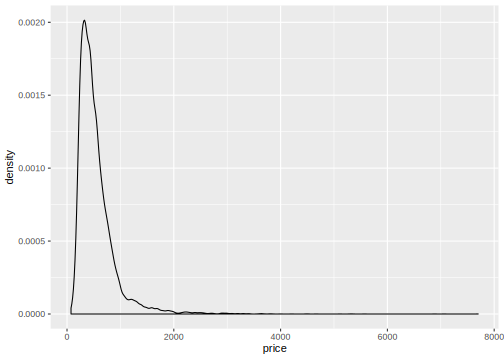
\includegraphics{mlr3book_files/figure-latex/09-use-cases-007-1} \end{center}

We can see that the prices for most houses lie between 75.000 and 1.5 million dollars.
There are few extreme values of up to 7.7 million dollars.

Feature engineering often allows us to incorporate additional knowledge about the data and underlying processes.
This can often greatly enhance predictive performance.
A simple example: A house which has \texttt{yr\_renovated\ ==\ 0} means that is has not been renovated yet.
Additionally we want to drop features which should not have any influence (\texttt{id\ column}).

After those initial manipulations, we load all required packages and create a Task containing our data.

\begin{Shaded}
\begin{Highlighting}[]
\KeywordTok{library}\NormalTok{(mlr3)}
\KeywordTok{library}\NormalTok{(mlr3viz)}
\NormalTok{tsk =}\StringTok{ }\NormalTok{TaskRegr}\OperatorTok{$}\KeywordTok{new}\NormalTok{(}\StringTok{"sales"}\NormalTok{, house_sales_prediction, }\DataTypeTok{target =} \StringTok{"price"}\NormalTok{)}
\end{Highlighting}
\end{Shaded}

We can inspect associations between variables using \href{https://mlr3viz.mlr-org.com}{mlr3viz}'s \texttt{autoplot} function in order to get some good first impressions for our data.
Note, that this does in no way prevent us from using other powerful plot functions of our choice on the original data.

\hypertarget{distribution-of-the-price}{%
\subsubsection{Distribution of the price:}\label{distribution-of-the-price}}

The outcome we want to predict is the \textbf{price} variable.
The \texttt{autoplot} function provides a good first glimpse on our data.
As the resulting object is a \texttt{ggplot2} object, we can use \texttt{faceting} and other functions from \textbf{ggplot2} in order to enhance plots.

\begin{Shaded}
\begin{Highlighting}[]
\KeywordTok{library}\NormalTok{(ggplot2)}
\KeywordTok{autoplot}\NormalTok{(tsk) }\OperatorTok{+}\StringTok{ }\KeywordTok{facet_wrap}\NormalTok{(}\OperatorTok{~}\NormalTok{renovated)}
\end{Highlighting}
\end{Shaded}

\begin{center}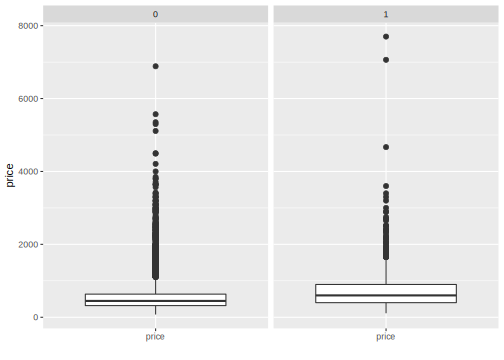
\includegraphics{mlr3book_files/figure-latex/09-use-cases-009-1} \end{center}

We can observe that renovated flats seem to achieve higher sales values, and this might thus be a relevant feature.

Additionally, we can for example look at the condition of the house.
Again, we clearly can see that the price rises with increasing condition.

\begin{Shaded}
\begin{Highlighting}[]
\KeywordTok{autoplot}\NormalTok{(tsk) }\OperatorTok{+}\StringTok{ }\KeywordTok{facet_wrap}\NormalTok{(}\OperatorTok{~}\NormalTok{condition)}
\end{Highlighting}
\end{Shaded}

\begin{center}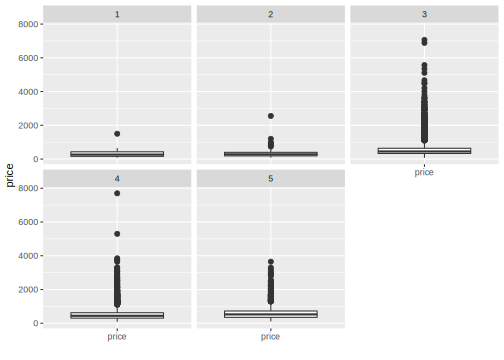
\includegraphics{mlr3book_files/figure-latex/09-use-cases-010-1} \end{center}

\hypertarget{association-between-variables}{%
\subsubsection{Association between variables}\label{association-between-variables}}

In addition to the association with the target variable, the association between the features can also lead to interesting insights.
We investigate using variables associated with the quality and size of the house.
Note that we use \texttt{\$clone()} and \texttt{\$select()} to clone the task and select only a subset of the features for the \texttt{autoplot} function, as \texttt{autoplot} per default uses all features.
The task is cloned before we select features in order to keep the original task intact.

\begin{Shaded}
\begin{Highlighting}[]
\CommentTok{# Variables associated with quality}
\KeywordTok{autoplot}\NormalTok{(tsk}\OperatorTok{$}\KeywordTok{clone}\NormalTok{()}\OperatorTok{$}\KeywordTok{select}\NormalTok{(tsk}\OperatorTok{$}\NormalTok{feature_names[}\KeywordTok{c}\NormalTok{(}\DecValTok{3}\NormalTok{, }\DecValTok{17}\NormalTok{)]), }
  \DataTypeTok{type =} \StringTok{"pairs"}\NormalTok{)}
\end{Highlighting}
\end{Shaded}

\begin{center}\includegraphics{mlr3book_files/figure-latex/09-use-cases-011-1} \end{center}

\begin{Shaded}
\begin{Highlighting}[]
\KeywordTok{autoplot}\NormalTok{(tsk}\OperatorTok{$}\KeywordTok{clone}\NormalTok{()}\OperatorTok{$}\KeywordTok{select}\NormalTok{(tsk}\OperatorTok{$}\NormalTok{feature_names[}\KeywordTok{c}\NormalTok{(}\DecValTok{9}\OperatorTok{:}\DecValTok{12}\NormalTok{)]), }
  \DataTypeTok{type =} \StringTok{"pairs"}\NormalTok{)}
\end{Highlighting}
\end{Shaded}

\begin{center}\includegraphics{mlr3book_files/figure-latex/09-use-cases-012-1} \end{center}

\hypertarget{splitting-into-train-and-test-data}{%
\subsection{Splitting into train and test data}\label{splitting-into-train-and-test-data}}

In \href{https://mlr3.mlr-org.com}{mlr3}, we do not create \texttt{train} and \texttt{test} data sets, but instead keep only a vector of train and test indices.

\begin{Shaded}
\begin{Highlighting}[]
\KeywordTok{set.seed}\NormalTok{(}\DecValTok{4411}\NormalTok{)}
\NormalTok{train.idx =}\StringTok{ }\KeywordTok{sample}\NormalTok{(}\KeywordTok{seq_len}\NormalTok{(tsk}\OperatorTok{$}\NormalTok{nrow), }\FloatTok{0.7} \OperatorTok{*}\StringTok{ }\NormalTok{tsk}\OperatorTok{$}\NormalTok{nrow)}
\NormalTok{test.idx =}\StringTok{ }\KeywordTok{setdiff}\NormalTok{(}\KeywordTok{seq_len}\NormalTok{(tsk}\OperatorTok{$}\NormalTok{nrow), train.idx)}
\end{Highlighting}
\end{Shaded}

\hypertarget{a-first-model-decision-tree}{%
\subsection{A first model: Decision Tree}\label{a-first-model-decision-tree}}

Decision trees cannot only be used as a powerful tool for predictive models but also for exploratory data analysis.
In order to fit a decision tree, we first get the \texttt{regr.rpart} learner from the \texttt{mlr\_learners} dictionary by using the sugar function \texttt{lrn}.

For now we leave out the \texttt{zipcode} variable, as we also have the \texttt{latitude} and \texttt{longitude} of each house.

\begin{Shaded}
\begin{Highlighting}[]
\NormalTok{tsk_nozip =}\StringTok{ }\NormalTok{tsk}\OperatorTok{$}\KeywordTok{clone}\NormalTok{()}\OperatorTok{$}\KeywordTok{select}\NormalTok{(}\KeywordTok{setdiff}\NormalTok{(tsk}\OperatorTok{$}\NormalTok{feature_names, }
  \StringTok{"zipcode"}\NormalTok{))}
\CommentTok{# Get the learner}
\NormalTok{lrn =}\StringTok{ }\KeywordTok{lrn}\NormalTok{(}\StringTok{"regr.rpart"}\NormalTok{)}
\CommentTok{# And train on the task}
\NormalTok{lrn}\OperatorTok{$}\KeywordTok{train}\NormalTok{(tsk_nozip, }\DataTypeTok{row_ids =}\NormalTok{ train.idx)}
\end{Highlighting}
\end{Shaded}

\begin{Shaded}
\begin{Highlighting}[]
\KeywordTok{plot}\NormalTok{(lrn}\OperatorTok{$}\NormalTok{model)}
\KeywordTok{text}\NormalTok{(lrn}\OperatorTok{$}\NormalTok{model)}
\end{Highlighting}
\end{Shaded}

\begin{center}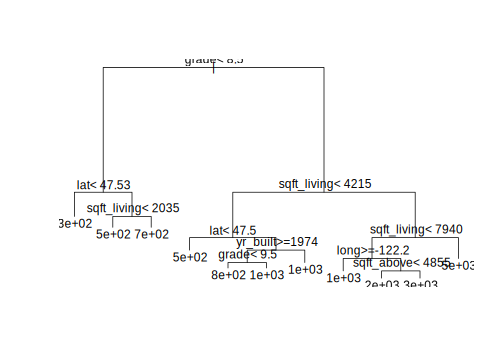
\includegraphics{mlr3book_files/figure-latex/09-use-cases-015-1} \end{center}

The learned tree relies on several variables in order to distinguish between cheaper and pricier houses.
The features we split along are \textbf{grade}, \textbf{sqft\_living}, but also some features related to the area (longitude and latitude).

We can visualize the price across different regions in order to get more info:

\begin{Shaded}
\begin{Highlighting}[]
\CommentTok{# Load the ggmap package in order to visualize on a map}
\KeywordTok{library}\NormalTok{(ggmap)}

\CommentTok{# And create a quick plot for the price}
\KeywordTok{qmplot}\NormalTok{(long, lat, }\DataTypeTok{maptype =} \StringTok{"watercolor"}\NormalTok{, }\DataTypeTok{color =} \KeywordTok{log}\NormalTok{(price), }
  \DataTypeTok{data =}\NormalTok{ house_sales_prediction[train.idx[}\DecValTok{1}\OperatorTok{:}\DecValTok{3000}\NormalTok{], ]) }\OperatorTok{+}\StringTok{ }
\StringTok{  }\KeywordTok{scale_colour_viridis_c}\NormalTok{()}
\end{Highlighting}
\end{Shaded}

\begin{center}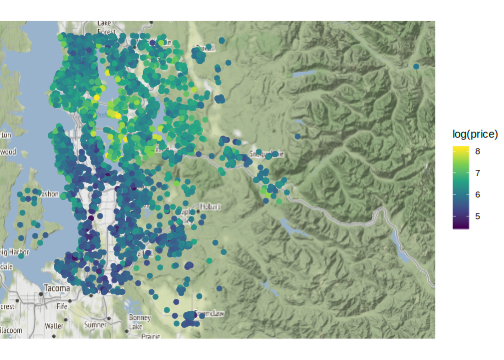
\includegraphics{mlr3book_files/figure-latex/09-use-cases-016-1} \end{center}

\begin{Shaded}
\begin{Highlighting}[]

\CommentTok{# And the zipcode}
\KeywordTok{qmplot}\NormalTok{(long, lat, }\DataTypeTok{maptype =} \StringTok{"watercolor"}\NormalTok{, }\DataTypeTok{color =}\NormalTok{ zipcode, }
  \DataTypeTok{data =}\NormalTok{ house_sales_prediction[train.idx[}\DecValTok{1}\OperatorTok{:}\DecValTok{3000}\NormalTok{], ]) }\OperatorTok{+}\StringTok{ }
\StringTok{  }\KeywordTok{guides}\NormalTok{(}\DataTypeTok{color =} \OtherTok{FALSE}\NormalTok{)}
\end{Highlighting}
\end{Shaded}

\begin{center}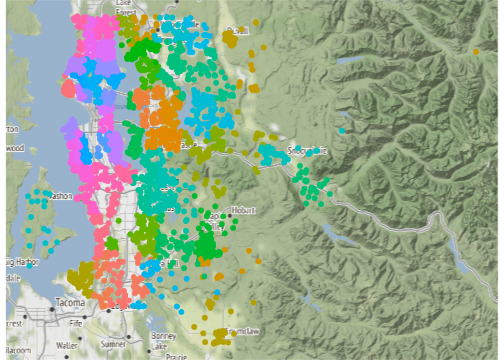
\includegraphics{mlr3book_files/figure-latex/09-use-cases-016-2} \end{center}

We can see that the price is clearly associated with the zipcode when comparing then two plots.
As a result, we might want to indeed use the \textbf{zipcode} column in our future endeavours.

\hypertarget{a-first-baseline-decision-tree}{%
\subsection{A first baseline: Decision Tree}\label{a-first-baseline-decision-tree}}

After getting an initial idea for our data, we might want to construct a first baseline, in order to see what a simple model already can achieve.

We use \texttt{resample} with \texttt{3-fold\ cross-validation} on our training data in order to get a reliable estimate of the algorithm's performance on future data.
Before we start with defining and training learners, we create a \texttt{Resampling} in order to make sure that we always compare on exactly the same data.

\begin{Shaded}
\begin{Highlighting}[]
\KeywordTok{library}\NormalTok{(mlr3learners)}
\NormalTok{cv3 =}\StringTok{ }\KeywordTok{rsmp}\NormalTok{(}\StringTok{"cv"}\NormalTok{, }\DataTypeTok{folds =} \DecValTok{3}\NormalTok{)}
\NormalTok{cv3}\OperatorTok{$}\KeywordTok{instantiate}\NormalTok{(tsk}\OperatorTok{$}\KeywordTok{clone}\NormalTok{()}\OperatorTok{$}\KeywordTok{filter}\NormalTok{(train.idx))}
\end{Highlighting}
\end{Shaded}

For the cross-validation we only use the \textbf{training data} by cloning the task and selecting only observations from the training set.

\begin{Shaded}
\begin{Highlighting}[]
\NormalTok{lrn_rpart =}\StringTok{ }\KeywordTok{lrn}\NormalTok{(}\StringTok{"regr.rpart"}\NormalTok{)}
\NormalTok{res =}\StringTok{ }\KeywordTok{resample}\NormalTok{(}\DataTypeTok{task =}\NormalTok{ tsk}\OperatorTok{$}\KeywordTok{clone}\NormalTok{()}\OperatorTok{$}\KeywordTok{filter}\NormalTok{(train.idx), lrn_rpart, }
\NormalTok{  cv3)}
\NormalTok{res}\OperatorTok{$}\KeywordTok{score}\NormalTok{(}\KeywordTok{msr}\NormalTok{(}\StringTok{"regr.mse"}\NormalTok{))}
\NormalTok{##          task task_id            learner learner_id}
\NormalTok{## 1: <TaskRegr>   sales <LearnerRegrRpart> regr.rpart}
\NormalTok{## 2: <TaskRegr>   sales <LearnerRegrRpart> regr.rpart}
\NormalTok{## 3: <TaskRegr>   sales <LearnerRegrRpart> regr.rpart}
\NormalTok{##        resampling resampling_id iteration prediction}
\NormalTok{## 1: <ResamplingCV>            cv         1     <list>}
\NormalTok{## 2: <ResamplingCV>            cv         2     <list>}
\NormalTok{## 3: <ResamplingCV>            cv         3     <list>}
\NormalTok{##    regr.mse}
\NormalTok{## 1:    45416}
\NormalTok{## 2:    49599}
\NormalTok{## 3:    42518}
\KeywordTok{sprintf}\NormalTok{(}\StringTok{"RMSE of the simple rpart: %s"}\NormalTok{, }\KeywordTok{round}\NormalTok{(}\KeywordTok{sqrt}\NormalTok{(res}\OperatorTok{$}\KeywordTok{aggregate}\NormalTok{()), }
  \DecValTok{2}\NormalTok{))}
\NormalTok{## [1] "RMSE of the simple rpart: 214.11"}
\end{Highlighting}
\end{Shaded}

\hypertarget{many-trees-random-forest}{%
\subsection{Many Trees: Random Forest}\label{many-trees-random-forest}}

We might be able to improve upon the \textbf{RMSE} using more powerful learners.
We first load the \href{https://mlr3learners.mlr-org.com}{mlr3learners} package, which contains the \textbf{ranger} learner (a package which implements the ``Random Forest'' algorithm).

\begin{Shaded}
\begin{Highlighting}[]
\NormalTok{lrn_ranger =}\StringTok{ }\KeywordTok{lrn}\NormalTok{(}\StringTok{"regr.ranger"}\NormalTok{, }\DataTypeTok{num.trees =}\NormalTok{ 15L)}
\NormalTok{res =}\StringTok{ }\KeywordTok{resample}\NormalTok{(}\DataTypeTok{task =}\NormalTok{ tsk}\OperatorTok{$}\KeywordTok{clone}\NormalTok{()}\OperatorTok{$}\KeywordTok{filter}\NormalTok{(train.idx), lrn_ranger, }
\NormalTok{  cv3)}
\NormalTok{res}\OperatorTok{$}\KeywordTok{score}\NormalTok{(}\KeywordTok{msr}\NormalTok{(}\StringTok{"regr.mse"}\NormalTok{))}
\NormalTok{##          task task_id             learner  learner_id}
\NormalTok{## 1: <TaskRegr>   sales <LearnerRegrRanger> regr.ranger}
\NormalTok{## 2: <TaskRegr>   sales <LearnerRegrRanger> regr.ranger}
\NormalTok{## 3: <TaskRegr>   sales <LearnerRegrRanger> regr.ranger}
\NormalTok{##        resampling resampling_id iteration prediction}
\NormalTok{## 1: <ResamplingCV>            cv         1     <list>}
\NormalTok{## 2: <ResamplingCV>            cv         2     <list>}
\NormalTok{## 3: <ResamplingCV>            cv         3     <list>}
\NormalTok{##    regr.mse}
\NormalTok{## 1:    23892}
\NormalTok{## 2:    22455}
\NormalTok{## 3:    18899}
\KeywordTok{sprintf}\NormalTok{(}\StringTok{"RMSE of the simple ranger: %s"}\NormalTok{, }\KeywordTok{round}\NormalTok{(}\KeywordTok{sqrt}\NormalTok{(res}\OperatorTok{$}\KeywordTok{aggregate}\NormalTok{()), }
  \DecValTok{2}\NormalTok{))}
\NormalTok{## [1] "RMSE of the simple ranger: 147.48"}
\end{Highlighting}
\end{Shaded}

Often tuning \textbf{RandomForest} methods does not increase predictive performances substantially.
If time permits, it can nonetheless lead to improvements and should thus be performed.
In this case, we resort to tune a different kind of model: \textbf{Gradient Boosted Decision Trees} from the package \texttt{xgboost}.

\hypertarget{a-better-baseline-autotuner}{%
\subsection{\texorpdfstring{A better baseline: \texttt{AutoTuner}}{A better baseline: AutoTuner}}\label{a-better-baseline-autotuner}}

Tuning can often further improve the performance.
In this case, we \emph{tune} the xgboost learner in order to see whether this can improve performance.
For the \texttt{AutoTuner} we have to specify a \textbf{Termination Criterion} (how long the tuning should run) a \textbf{Tuner} (which tuning method to use) and a \textbf{ParamSet} (which space we might want to search through).
For now we do not use the \textbf{zipcode} column, as \texttt{xgboost} cannot naturally
deal with categorical features.
The \textbf{AutoTuner} automatically performs nested cross-validation.

\begin{Shaded}
\begin{Highlighting}[]
\KeywordTok{set.seed}\NormalTok{(444L)}
\KeywordTok{library}\NormalTok{(mlr3tuning)}
\KeywordTok{library}\NormalTok{(paradox)}
\NormalTok{lrn_xgb =}\StringTok{ }\KeywordTok{lrn}\NormalTok{(}\StringTok{"regr.xgboost"}\NormalTok{)}

\CommentTok{# Define the ParamSet}
\NormalTok{ps =}\StringTok{ }\NormalTok{ParamSet}\OperatorTok{$}\KeywordTok{new}\NormalTok{(}\DataTypeTok{params =} \KeywordTok{list}\NormalTok{(ParamDbl}\OperatorTok{$}\KeywordTok{new}\NormalTok{(}\DataTypeTok{id =} \StringTok{"eta"}\NormalTok{, }
  \DataTypeTok{lower =} \FloatTok{0.2}\NormalTok{, }\DataTypeTok{upper =} \FloatTok{0.4}\NormalTok{), ParamDbl}\OperatorTok{$}\KeywordTok{new}\NormalTok{(}\DataTypeTok{id =} \StringTok{"min_child_weight"}\NormalTok{, }
  \DataTypeTok{lower =} \DecValTok{1}\NormalTok{, }\DataTypeTok{upper =} \DecValTok{20}\NormalTok{), ParamDbl}\OperatorTok{$}\KeywordTok{new}\NormalTok{(}\DataTypeTok{id =} \StringTok{"subsample"}\NormalTok{, }
  \DataTypeTok{lower =} \FloatTok{0.7}\NormalTok{, }\DataTypeTok{upper =} \FloatTok{0.8}\NormalTok{), ParamDbl}\OperatorTok{$}\KeywordTok{new}\NormalTok{(}\DataTypeTok{id =} \StringTok{"colsample_bytree"}\NormalTok{, }
  \DataTypeTok{lower =} \FloatTok{0.9}\NormalTok{, }\DataTypeTok{upper =} \DecValTok{1}\NormalTok{), ParamDbl}\OperatorTok{$}\KeywordTok{new}\NormalTok{(}\DataTypeTok{id =} \StringTok{"colsample_bylevel"}\NormalTok{, }
  \DataTypeTok{lower =} \FloatTok{0.5}\NormalTok{, }\DataTypeTok{upper =} \FloatTok{0.7}\NormalTok{), ParamInt}\OperatorTok{$}\KeywordTok{new}\NormalTok{(}\DataTypeTok{id =} \StringTok{"nrounds"}\NormalTok{, }
  \DataTypeTok{lower =}\NormalTok{ 1L, }\DataTypeTok{upper =} \DecValTok{25}\NormalTok{)))}

\CommentTok{# Define the Terminator}
\NormalTok{terminator =}\StringTok{ }\NormalTok{TerminatorEvaluations}\OperatorTok{$}\KeywordTok{new}\NormalTok{(}\DecValTok{10}\NormalTok{)}
\NormalTok{cv3 =}\StringTok{ }\KeywordTok{rsmp}\NormalTok{(}\StringTok{"cv"}\NormalTok{, }\DataTypeTok{folds =} \DecValTok{3}\NormalTok{)}
\NormalTok{at =}\StringTok{ }\NormalTok{AutoTuner}\OperatorTok{$}\KeywordTok{new}\NormalTok{(lrn_xgb, cv3, }\DataTypeTok{measures =} \KeywordTok{msr}\NormalTok{(}\StringTok{"regr.mse"}\NormalTok{), }
\NormalTok{  ps, terminator, }\DataTypeTok{tuner =}\NormalTok{ TunerRandomSearch, }\DataTypeTok{tuner_settings =} \KeywordTok{list}\NormalTok{())}
\end{Highlighting}
\end{Shaded}

\begin{Shaded}
\begin{Highlighting}[]
\NormalTok{res}\OperatorTok{$}\KeywordTok{score}\NormalTok{(}\KeywordTok{msr}\NormalTok{(}\StringTok{"regr.mse"}\NormalTok{))}
\KeywordTok{sprintf}\NormalTok{(}\StringTok{"RMSE of the tuned xgboost: %s"}\NormalTok{, }\KeywordTok{round}\NormalTok{(}\KeywordTok{sqrt}\NormalTok{(res}\OperatorTok{$}\KeywordTok{aggregate}\NormalTok{()), }
  \DecValTok{2}\NormalTok{))}
\end{Highlighting}
\end{Shaded}

We can obtain the resulting params in the respective splits by accessing the \texttt{ResampleResult}.

\begin{Shaded}
\begin{Highlighting}[]
\KeywordTok{sapply}\NormalTok{(res}\OperatorTok{$}\NormalTok{learners, }\ControlFlowTok{function}\NormalTok{(x) x}\OperatorTok{$}\NormalTok{param_set}\OperatorTok{$}\NormalTok{values)}
\NormalTok{## $num.trees}
\NormalTok{## [1] 15}
\NormalTok{## }
\NormalTok{## $num.trees}
\NormalTok{## [1] 15}
\NormalTok{## }
\NormalTok{## $num.trees}
\NormalTok{## [1] 15}
\end{Highlighting}
\end{Shaded}

\textbf{NOTE:} To keep runtime low, we only tune parts of the hyperparameter space of \texttt{xgboost} in this example.
Additionally, we only allow for \(10\) random search iterations, which is usually to little for real-world applications.
Nonetheless, we are able to obtain an improved performance when comparing to the \texttt{ranger} model.

In order to further improve our results we have several options:

\begin{itemize}
\tightlist
\item
  Find or engineer better features
\item
  Remove Features to avoid overfitting
\item
  Obtain additional data (often prohibitive)
\item
  Try more models
\item
  Improve the tuning

  \begin{itemize}
  \tightlist
  \item
    Increase the tuning budget
  \item
    Enlarge the tuning search space
  \item
    Use a more efficient tuning algorithm
  \end{itemize}
\item
  Stacking and Ensembles (see \protect\hyperlink{pipelines}{Pipelines})
\end{itemize}

Below we will investigate some of those possibilities and investigate whether this improves performance.

\hypertarget{engineering-features-mutating-zip-codes}{%
\subsection{Engineering Features: Mutating ZIP-Codes}\label{engineering-features-mutating-zip-codes}}

In order to better cluster the zip codes, we compute a new feature: \textbf{med\_price}:
It computes the median price in each zip-code.
This might help our model to improve the prediction.

\begin{Shaded}
\begin{Highlighting}[]
\CommentTok{# Create a new feature and append it to the task}
\NormalTok{zip_price =}\StringTok{ }\NormalTok{house_sales_prediction[, .(}\DataTypeTok{med_price =} \KeywordTok{median}\NormalTok{(price)), }
\NormalTok{  by =}\StringTok{ }\NormalTok{zipcode]}

\CommentTok{# Join on the original data to match with original}
\CommentTok{# columns, then cbind to the task}
\NormalTok{tsk}\OperatorTok{$}\KeywordTok{cbind}\NormalTok{(house_sales_prediction[zip_price, }\DataTypeTok{on =} \StringTok{"zipcode"}\NormalTok{][, }
  \StringTok{"med_price"}\NormalTok{])}
\end{Highlighting}
\end{Shaded}

Again, we run \texttt{resample} and compute the \textbf{RMSE}.

\begin{Shaded}
\begin{Highlighting}[]
\NormalTok{lrn_ranger =}\StringTok{ }\KeywordTok{lrn}\NormalTok{(}\StringTok{"regr.ranger"}\NormalTok{)}
\NormalTok{res =}\StringTok{ }\KeywordTok{resample}\NormalTok{(}\DataTypeTok{task =}\NormalTok{ tsk}\OperatorTok{$}\KeywordTok{clone}\NormalTok{()}\OperatorTok{$}\KeywordTok{filter}\NormalTok{(train.idx), lrn_ranger, }
\NormalTok{  cv3)}
\NormalTok{res}\OperatorTok{$}\KeywordTok{score}\NormalTok{(}\KeywordTok{msr}\NormalTok{(}\StringTok{"regr.mse"}\NormalTok{))}
\NormalTok{##          task task_id             learner  learner_id}
\NormalTok{## 1: <TaskRegr>   sales <LearnerRegrRanger> regr.ranger}
\NormalTok{## 2: <TaskRegr>   sales <LearnerRegrRanger> regr.ranger}
\NormalTok{## 3: <TaskRegr>   sales <LearnerRegrRanger> regr.ranger}
\NormalTok{##        resampling resampling_id iteration prediction}
\NormalTok{## 1: <ResamplingCV>            cv         1     <list>}
\NormalTok{## 2: <ResamplingCV>            cv         2     <list>}
\NormalTok{## 3: <ResamplingCV>            cv         3     <list>}
\NormalTok{##    regr.mse}
\NormalTok{## 1:    22719}
\NormalTok{## 2:    20384}
\NormalTok{## 3:    17799}
\KeywordTok{sprintf}\NormalTok{(}\StringTok{"RMSE of ranger with med_price: %s"}\NormalTok{, }\KeywordTok{round}\NormalTok{(}\KeywordTok{sqrt}\NormalTok{(res}\OperatorTok{$}\KeywordTok{aggregate}\NormalTok{()), }
  \DecValTok{2}\NormalTok{))}
\NormalTok{## [1] "RMSE of ranger with med_price: 142.48"}
\end{Highlighting}
\end{Shaded}

\hypertarget{obtaining-a-sparser-model}{%
\subsection{Obtaining a sparser model}\label{obtaining-a-sparser-model}}

In many cases, we might want to have a sparse model.
For this purpose we can use a \texttt{mlr3filters::Filter} implemented in \href{https://mlr3filters.mlr-org.com}{mlr3filters}.
This can prevent our learner from overfitting make it easier for humans to interpret models as fewer variables influence the resulting prediction.

\begin{Shaded}
\begin{Highlighting}[]
\KeywordTok{library}\NormalTok{(mlr3filters)}
\NormalTok{filter =}\StringTok{ }\NormalTok{FilterMRMR}\OperatorTok{$}\KeywordTok{new}\NormalTok{()}\OperatorTok{$}\KeywordTok{calculate}\NormalTok{(tsk)}
\NormalTok{tsk_ftsel =}\StringTok{ }\NormalTok{tsk}\OperatorTok{$}\KeywordTok{clone}\NormalTok{()}\OperatorTok{$}\KeywordTok{select}\NormalTok{(}\KeywordTok{head}\NormalTok{(}\KeywordTok{names}\NormalTok{(filter}\OperatorTok{$}\NormalTok{scores), }
  \DecValTok{12}\NormalTok{))}
\end{Highlighting}
\end{Shaded}

The resulting \textbf{RMSE} is slightly higher, and at the same time we only use \(12\) features.

\begin{Shaded}
\begin{Highlighting}[]
\NormalTok{lrn_ranger =}\StringTok{ }\KeywordTok{lrn}\NormalTok{(}\StringTok{"regr.ranger"}\NormalTok{)}
\NormalTok{res =}\StringTok{ }\KeywordTok{resample}\NormalTok{(}\DataTypeTok{task =}\NormalTok{ tsk_ftsel}\OperatorTok{$}\KeywordTok{clone}\NormalTok{()}\OperatorTok{$}\KeywordTok{filter}\NormalTok{(train.idx), }
\NormalTok{  lrn_ranger, cv3)}
\NormalTok{res}\OperatorTok{$}\KeywordTok{score}\NormalTok{(}\KeywordTok{msr}\NormalTok{(}\StringTok{"regr.mse"}\NormalTok{))}
\NormalTok{##          task task_id             learner  learner_id}
\NormalTok{## 1: <TaskRegr>   sales <LearnerRegrRanger> regr.ranger}
\NormalTok{## 2: <TaskRegr>   sales <LearnerRegrRanger> regr.ranger}
\NormalTok{## 3: <TaskRegr>   sales <LearnerRegrRanger> regr.ranger}
\NormalTok{##        resampling resampling_id iteration prediction}
\NormalTok{## 1: <ResamplingCV>            cv         1     <list>}
\NormalTok{## 2: <ResamplingCV>            cv         2     <list>}
\NormalTok{## 3: <ResamplingCV>            cv         3     <list>}
\NormalTok{##    regr.mse}
\NormalTok{## 1:    34720}
\NormalTok{## 2:    29056}
\NormalTok{## 3:    25907}
\KeywordTok{sprintf}\NormalTok{(}\StringTok{"RMSE of ranger with filtering: %s"}\NormalTok{, }\KeywordTok{round}\NormalTok{(}\KeywordTok{sqrt}\NormalTok{(res}\OperatorTok{$}\KeywordTok{aggregate}\NormalTok{()), }
  \DecValTok{2}\NormalTok{))}
\NormalTok{## [1] "RMSE of ranger with filtering: 172.9"}
\end{Highlighting}
\end{Shaded}

\hypertarget{appendix}{%
\chapter{Appendix}\label{appendix}}

\hypertarget{list-learners}{%
\section{Integrated Learners}\label{list-learners}}

\includegraphics[width=8.50in,height=8.58in,keepaspectratio]{mlr3book_files/figure-latex/98-appendix-001-1.png}

\hypertarget{list-measures}{%
\section{Integrated Performance Measures}\label{list-measures}}

Also see the \href{https://mlr3measures.mlr-org.com/reference/}{overview on the website} of \href{https://mlr3measures.mlr-org.com}{mlr3measures}.

\includegraphics[width=5.50in,height=9.49in,keepaspectratio]{mlr3book_files/figure-latex/98-appendix-002-1.png}

\hypertarget{list-filters}{%
\section{Integrated Filter Methods}\label{list-filters}}

\hypertarget{fs-filter-list}{%
\subsection{Standalone filter methods}\label{fs-filter-list}}

\includegraphics[width=7.00in,height=3.74in,keepaspectratio]{mlr3book_files/figure-latex/98-appendix-003-1.png}

\hypertarget{fs-filter-embedded-list}{%
\subsection{Algorithms With Embedded Filter Methods}\label{fs-filter-embedded-list}}

\begin{verbatim}
##  [1] "classif.featureless"  "classif.ranger"      
##  [3] "classif.rpart"        "classif.xgboost"     
##  [5] "regr.featureless"     "regr.ranger"         
##  [7] "regr.rpart"           "regr.xgboost"        
##  [9] "surv.coxph"           "surv.gbm"            
## [11] "surv.penalized"       "surv.randomForestSRC"
## [13] "surv.ranger"          "surv.rpart"
\end{verbatim}

\hypertarget{references}{%
\chapter{References}\label{references}}

\hypertarget{refs}{}
\leavevmode\hypertarget{ref-bergstra2012}{}%
Bergstra, James, and Yoshua Bengio. 2012. ``Random Search for Hyper-Parameter Optimization.'' \emph{J. Mach. Learn. Res.} 13. JMLR.org: 281--305.

\leavevmode\hypertarget{ref-mlr}{}%
Bischl, Bernd, Michel Lang, Lars Kotthoff, Julia Schiffner, Jakob Richter, Erich Studerus, Giuseppe Casalicchio, and Zachary M. Jones. 2016. ``mlr: Machine Learning in R.'' \emph{Journal of Machine Learning Research} 17 (170): 1--5. \url{http://jmlr.org/papers/v17/15-066.html}.

\leavevmode\hypertarget{ref-Breiman1996}{}%
Breiman, Leo. 1996. ``Bagging Predictors.'' \emph{Machine Learning} 24 (2). Springer: 123--40.

\leavevmode\hypertarget{ref-chandrashekar2014}{}%
Chandrashekar, Girish, and Ferat Sahin. 2014. ``A Survey on Feature Selection Methods.'' \emph{Computers and Electrical Engineering} 40 (1): 16--28. \url{https://doi.org/https://doi.org/10.1016/j.compeleceng.2013.11.024}.

\leavevmode\hypertarget{ref-checkmate}{}%
Lang, Michel. 2017. ``checkmate: Fast Argument Checks for Defensive R Programming.'' \emph{The R Journal} 9 (1): 437--45. \url{https://doi.org/10.32614/RJ-2017-028}.

\leavevmode\hypertarget{ref-mlr3}{}%
Lang, Michel, Martin Binder, Jakob Richter, Patrick Schratz, Florian Pfisterer, Stefan Coors, Quay Au, Giuseppe Casalicchio, Lars Kotthoff, and Bernd Bischl. 2019. ``mlr3: A Modern Object-Oriented Machine Learning Framework in R.'' \emph{Journal of Open Source Software}, December. \url{https://doi.org/10.21105/joss.01903}.

\leavevmode\hypertarget{ref-R}{}%
R Core Team. 2019. \emph{R: A Language and Environment for Statistical Computing}. Vienna, Austria: R Foundation for Statistical Computing. \url{https://www.R-project.org/}.

\leavevmode\hypertarget{ref-Wolpert1992}{}%
Wolpert, David H. 1992. ``Stacked Generalization.'' \emph{Neural Networks} 5 (2): 241--59. \url{https://doi.org/https://doi.org/10.1016/S0893-6080(05)80023-1}.

\end{document}
